\documentclass[11pt,fleqn]{book} % Default font size and left-justified equations
% TEMPLATE ADAPTED FROM: copyright 2014 Andrea Hidalgo

\usepackage[top=2.5cm,bottom=2.8cm,left=3cm,right=3cm,headsep=10pt,a4paper]{geometry} % Page margins

\usepackage{xcolor} % Required for specifying colors by name
\definecolor{ocre}{RGB}{52,177,201} % Define the orange color used for highlighting throughout the book
% Font Settings
\usepackage{avant} % Use the Avantgarde font for headings
%\usepackage{times} % Use the Times font for headings
\usepackage{mathptmx} % Use the Adobe Times Roman as the default text font together with math symbols from the Sym­bol, Chancery and Com­puter Modern fonts
\usepackage{microtype} % Slightly tweak font spacing for aesthetics
\usepackage[utf8]{inputenc} % Required for including letters with accents
\usepackage[T1]{fontenc} % Use 8-bit encoding that has 256 glyphs
\usepackage{amsthm, amssymb, amsmath}
\usepackage{accents}
\newcommand*{\dt}[1]{%
   \accentset{\mbox{\large\bfseries .}}{#1}}
\newcommand*{\ddt}[1]{%
   \accentset{\mbox{\large\bfseries ..}}{#1}}
\usepackage{calc}
\usepackage[italian]{babel}
\usepackage{bookmark}
\usepackage{float}
\usepackage[caption = false]{subfig}
\usepackage[labelfont=bf]{caption}

% Bibliography
\usepackage[style=alphabetic,sortcites=true,autopunct=true,babel=hyphen, citestyle=authoryear, hyperref=true,abbreviate=false,backref=true,backend=bibtex]{biblatex}
\addbibresource{bibliography.bib} % BibTeX bibliography file
\defbibheading{bibempty}{Bibliografia}

%----------------------------------------------------------------------------------------
%	VARIOUS REQUIRED PACKAGES
%----------------------------------------------------------------------------------------

\usepackage{titlesec} % Allows customization of titles

\usepackage{graphicx} % Required for including pictures
\graphicspath{{Pictures/}} % Specifies the directory where pictures are stored
% \graphicspath{{Plots/}}
\usepackage{lipsum} % Inserts dummy text

\usepackage{tikz} % Required for drawing custom shapes

%\usepackage[english]{babel} % English language/hyphenation

\usepackage{enumitem} % Customize lists
\setlist{nolistsep} % Reduce spacing between bullet points and numbered lists

\usepackage{booktabs} % Required for nicer horizontal rules in tables

\usepackage{eso-pic} % Required for specifying an image background in the title page

%----------------------------------------------------------------------------------------
%	MAIN TABLE OF CONTENTS
%----------------------------------------------------------------------------------------

\usepackage{titletoc} % Required for manipulating the table of contents

\contentsmargin{0cm} % Removes the default margin
% Chapter text styling
\titlecontents{chapter}[1.25cm] % Indentation
{\addvspace{15pt}\large\sffamily\bfseries} % Spacing and font options for chapters
{\color{ocre!60}\contentslabel[\Large\thecontentslabel]{1.25cm}\color{ocre}} % Chapter number
{}  
{\color{ocre!60}\normalsize\sffamily\bfseries\;\titlerule*[.5pc]{.}\;\thecontentspage} % Page number
% Section text styling
\titlecontents{section}[1.25cm] % Indentation
{\addvspace{5pt}\sffamily\bfseries} % Spacing and font options for sections
{\contentslabel[\thecontentslabel]{1.25cm}} % Section number
{}
{\sffamily\hfill\color{black}\thecontentspage} % Page number
[]
% Subsection text styling
\titlecontents{subsection}[1.25cm] % Indentation
{\addvspace{1pt}\sffamily\small} % Spacing and font options for subsections
{\contentslabel[\thecontentslabel]{1.25cm}} % Subsection number
{}
{\sffamily\;\titlerule*[.5pc]{.}\;\thecontentspage} % Page number
[] 

%----------------------------------------------------------------------------------------
%	MINI TABLE OF CONTENTS IN CHAPTER HEADS
%----------------------------------------------------------------------------------------

% Section text styling
\titlecontents{lsection}[0em] % Indendating
{\footnotesize\sffamily} % Font settings
{}
{}
{}

% Subsection text styling
\titlecontents{lsubsection}[.5em] % Indentation
{\normalfont\footnotesize\sffamily} % Font settings
{}
{}
{}
 
%----------------------------------------------------------------------------------------
%	PAGE HEADERS
%----------------------------------------------------------------------------------------

\usepackage{fancyhdr} % Required for header and footer configuration

\pagestyle{fancy}
\renewcommand{\chaptermark}[1]{\markboth{\sffamily\normalsize\bfseries\chaptername\ \thechapter.\ #1}{}} % Chapter text font settings
\renewcommand{\sectionmark}[1]{\markright{\sffamily\normalsize\thesection\hspace{5pt}#1}{}} % Section text font settings
\fancyhf{} \fancyhead[LE,RO]{\sffamily\normalsize\thepage} % Font setting for the page number in the header
\fancyhead[LO]{\rightmark} % Print the nearest section name on the left side of odd pages
\fancyhead[RE]{\leftmark} % Print the current chapter name on the right side of even pages
\renewcommand{\headrulewidth}{0.5pt} % Width of the rule under the header
\addtolength{\headheight}{2.5pt} % Increase the spacing around the header slightly
\renewcommand{\footrulewidth}{0pt} % Removes the rule in the footer
\fancypagestyle{plain}{\fancyhead{}\renewcommand{\headrulewidth}{0pt}} % Style for when a plain pagestyle is specified

% Removes the header from odd empty pages at the end of chapters
\makeatletter
\renewcommand{\cleardoublepage}{
\clearpage\ifodd\c@page\else
\hbox{}
\vspace*{\fill}
\thispagestyle{empty}
\newpage
\fi}

%----------------------------------------------------------------------------------------
%	THEOREM STYLES
%----------------------------------------------------------------------------------------

\usepackage{amsmath,amsfonts,amssymb,amsthm} % For math equations, theorems, symbols, etc

\newcommand{\intoo}[2]{\mathopen{]}#1\,;#2\mathclose{[}}
\newcommand{\ud}{\mathop{\mathrm{{}d}}\mathopen{}}
\newcommand{\intff}[2]{\mathopen{[}#1\,;#2\mathclose{]}}
\newtheorem{notation}{Notation}[chapter]

%%%%%%%%%%%%%%%%%%%%%%%%%%%%%%%%%%%%%%%%%%%%%%%%%%%%%%%%%%%%%%%%%%%%%%%%%%%
%%%%%%%%%%%%%%%%%%%% dedicated to boxed/framed environements %%%%%%%%%%%%%%
%%%%%%%%%%%%%%%%%%%%%%%%%%%%%%%%%%%%%%%%%%%%%%%%%%%%%%%%%%%%%%%%%%%%%%%%%%%
\newtheoremstyle{ocrenumbox}% % Theorem style name
{0pt}% Space above
{0pt}% Space below
{\normalfont}% % Body font
{}% Indent amount
{\small\bf\sffamily\color{ocre}}% % Theorem head font
{\;}% Punctuation after theorem head
{0.25em}% Space after theorem head
{\thmnote{\nobreakspace\the\thm@notefont\sffamily\bfseries\color{ocre}\nobreakspace#3.}} % Optional theorem note
\renewcommand{\qedsymbol}{$\blacksquare$}% Optional qed square

\newtheoremstyle{blacknumex}% Theorem style name
{5pt}% Space above
{5pt}% Space below
{\normalfont}% Body font
{} % Indent amount
{\small\bf\sffamily}% Theorem head font
{\;}% Punctuation after theorem head
{0.25em}% Space after theorem head
{\small\sffamily{\tiny\ensuremath{\blacksquare}}
\thmnote{\nobreakspace\the\thm@notefont\sffamily\bfseries\nobreakspace#3.}}% Optional theorem note

\newtheoremstyle{blacknumbox} % Theorem style name
{0pt}% Space above
{0pt}% Space below
{\normalfont}% Body font
{}% Indent amount
{\small\bf\sffamily}% Theorem head font
{\;}% Punctuation after theorem head
{0.25em}% Space after theorem head
{\thmnote{\nobreakspace\the\thm@notefont\sffamily\bfseries\nobreakspace#3.}}% Optional theorem note

%%%%%%%%%%%%%%%%%%%%%%%%%%%%%%%%%%%%%%%%%%%%%%%%%%%%%%%%%%%%%%%%%%%%%%%%%%%
%%%%%%%%%%%%% dedicated to non-boxed/non-framed environements %%%%%%%%%%%%%
%%%%%%%%%%%%%%%%%%%%%%%%%%%%%%%%%%%%%%%%%%%%%%%%%%%%%%%%%%%%%%%%%%%%%%%%%%%
\newtheoremstyle{ocrenum}% % Theorem style name
{5pt}% Space above
{5pt}% Space below
{\normalfont}% % Body font
{}% Indent amount
{\small\bf\sffamily\color{ocre}}% % Theorem head font
{\;}% Punctuation after theorem head
{0.25em}% Space after theorem head
{\small\sffamily\color{ocre}\thmname{#1}\nobreakspace\thmnumber{\@ifnotempty{#1}{}\@upn{#2}}% Theorem text (e.g. Theorem 2.1)
\thmnote{\nobreakspace\the\thm@notefont\sffamily\bfseries\color{black}---\nobreakspace#3.}} % Optional theorem note
\renewcommand{\qedsymbol}{$\blacksquare$}% Optional qed square
\makeatother

% Defines the theorem text style for each type of theorem to one of the three styles above
\newcounter{dummy} 
\numberwithin{dummy}{section}
\theoremstyle{ocrenumbox}


\newtheorem{theoremeT}[dummy]{Theorem}
\newtheorem{lemma}[dummy]{Lemma}
\newtheorem{observation}[dummy]{Observation}
\newtheorem{proposition}[dummy]{Proposition}
% \newtheorem{definition}[dummy]{Definition}
\newtheorem{claim}[dummy]{Claim}
\newtheorem{fact}[dummy]{Fact}
\newtheorem{assumption}[dummy]{Assumption}

\newtheorem{problem}{Problem}[chapter]
% \newtheorem{exercise}{Exercise}[chapter]
\theoremstyle{blacknumex}
\newtheorem{exampleT}{Example}[chapter]
\theoremstyle{blacknumbox}
\newtheorem{vocabulary}{Vocabulary}[chapter]
\newtheorem{definitionT}{Definition}[section]
\newtheorem{corollaryT}[dummy]{Corollary}
\theoremstyle{ocrenum}

%----------------------------------------------------------------------------------------
%	DEFINITION OF COLORED BOXES
%----------------------------------------------------------------------------------------

\RequirePackage[framemethod=default]{mdframed} % Required for creating the theorem, definition, exercise and corollary boxes

% Theorem box
\newmdenv[skipabove=7pt,
skipbelow=7pt,
backgroundcolor=black!5,
linecolor=ocre,
innerleftmargin=5pt,
innerrightmargin=5pt,
innertopmargin=5pt,
leftmargin=0cm,
rightmargin=0cm,
innerbottommargin=5pt]{tBox}

% Exercise box	  
\newmdenv[skipabove=7pt,
skipbelow=7pt,
rightline=false,
leftline=true,
topline=false,
bottomline=false,
backgroundcolor=ocre!10,
linecolor=ocre,
innerleftmargin=5pt,
innerrightmargin=5pt,
innertopmargin=5pt,
innerbottommargin=5pt,
leftmargin=0cm,
rightmargin=0cm,
linewidth=4pt]{eBox}	

% Definition box
\newmdenv[skipabove=7pt,
skipbelow=7pt,
rightline=false,
leftline=true,
topline=false,
bottomline=false,
linecolor=ocre,
innerleftmargin=5pt,
innerrightmargin=5pt,
innertopmargin=0pt,
leftmargin=0cm,
rightmargin=0cm,
linewidth=4pt,
innerbottommargin=0pt]{dBox}	

% Corollary box
\newmdenv[skipabove=7pt,
skipbelow=7pt,
rightline=false,
leftline=true,
topline=false,
bottomline=false,
linecolor=gray,
backgroundcolor=black!5,
innerleftmargin=5pt,
innerrightmargin=5pt,
innertopmargin=5pt,
leftmargin=0cm,
rightmargin=0cm,
linewidth=4pt,
innerbottommargin=5pt]{cBox}

% Creates an environment for each type of theorem and assigns it a theorem text style from the "Theorem Styles" section above and a colored box from above
\newenvironment{theorem}{\begin{tBox}\begin{theoremeT}}{\end{theoremeT}\end{tBox}}
\newenvironment{exercise}{\begin{eBox}\begin{exerciseT}}{\hfill{\color{ocre}\tiny\ensuremath{\blacksquare}}\end{exerciseT}\end{eBox}}				  
\newenvironment{definition}{\begin{dBox}\begin{definitionT}}{\end{definitionT}\end{dBox}}	
\newenvironment{example}{\begin{exampleT}}{\hfill{\tiny\ensuremath{}}\end{exampleT}}		
\newenvironment{corollary}{\begin{cBox}\begin{corollaryT}}{\end{corollaryT}\end{cBox}}	

%----------------------------------------------------------------------------------------
%	REMARK ENVIRONMENT
%----------------------------------------------------------------------------------------

\newenvironment{remark}{\par\vspace{10pt}\small % Vertical white space above the remark and smaller font size
\begin{list}{}{
\leftmargin=35pt % Indentation on the left
\rightmargin=25pt}\item\ignorespaces % Indentation on the right
\makebox[-2.5pt]{\begin{tikzpicture}[overlay]
\node[draw=ocre!60,line width=1pt,circle,fill=ocre!25,font=\sffamily\bfseries,inner sep=2pt,outer sep=0pt] at (-15pt,0pt){\textcolor{ocre}{R}};\end{tikzpicture}} % Orange R in a circle
\advance\baselineskip -1pt}{\end{list}\vskip5pt} % Tighter line spacing and white space after remark

%----------------------------------------------------------------------------------------
%	SECTION NUMBERING IN THE MARGIN
%----------------------------------------------------------------------------------------

\makeatletter
\renewcommand{\@seccntformat}[1]{\llap{\textcolor{ocre}{\csname the#1\endcsname}\hspace{1em}}}                    
\renewcommand{\section}{\@startsection{section}{1}{\z@}
{-4ex \@plus -1ex \@minus -.4ex}
{1ex \@plus.2ex }
{\normalfont\large\sffamily\bfseries}}
\renewcommand{\subsection}{\@startsection {subsection}{2}{\z@}
{-3ex \@plus -0.1ex \@minus -.4ex}
{0.5ex \@plus.2ex }
{\normalfont\sffamily\bfseries}}
\renewcommand{\subsubsection}{\@startsection {subsubsection}{3}{\z@}
{-2ex \@plus -0.1ex \@minus -.2ex}
{.2ex \@plus.2ex }
{\normalfont\small\sffamily\bfseries}}                        
\renewcommand\paragraph{\@startsection{paragraph}{4}{\z@}
{-2ex \@plus-.2ex \@minus .2ex}
{.1ex}
{\normalfont\small\sffamily\bfseries}}

%----------------------------------------------------------------------------------------
%	HYPERLINKS IN THE DOCUMENTS
%----------------------------------------------------------------------------------------

% For an unclear reason, the package should be loaded now and not later
\usepackage{hyperref}
%\hypersetup{hidelinks,backref=true,pagebackref=true,hyperindex=true,colorlinks=false,breaklinks=true,urlcolor= ocre,bookmarks=true,bookmarksopen=false,pdftitle={Title},pdfauthor={Author}}

%----------------------------------------------------------------------------------------
%	CHAPTER HEADINGS
%----------------------------------------------------------------------------------------

% The set-up below should be (sadly) manually adapted to the overall margin page septup controlled by the geometry package loaded in the main.tex document. It is possible to implement below the dimensions used in the goemetry package (top,bottom,left,right)... TO BE DONE

\newcommand{\thechapterimage}{}
\newcommand{\chapterimage}[1]{\renewcommand{\thechapterimage}{#1}}

% Numbered chapters with mini tableofcontents
\def\thechapter{\arabic{chapter}}
\def\@makechapterhead#1{
\thispagestyle{empty}
{\centering \normalfont\sffamily
\ifnum \c@secnumdepth >\m@ne
\if@mainmatter
\startcontents
\begin{tikzpicture}[remember picture,overlay]
\node at (current page.north west)
{\begin{tikzpicture}[remember picture,overlay]
\node[anchor=north west,inner sep=0pt] at (0,0) {\includegraphics[width=\paperwidth]{\thechapterimage}};
%%%%%%%%%%%%%%%%%%%%%%%%%%%%%%%%%%%%%%%%%%%%%%%%%%%%%%%%%%%%%%%%%%%%%%%%%%%%%%%%%%%%%
% Commenting the 3 lines below removes the small contents box in the chapter heading
%\fill[color=ocre!10!white,opacity=.6] (1cm,0) rectangle (8cm,-7cm);
%\node[anchor=north west] at (1.1cm,.35cm) {\parbox[t][8cm][t]{6.5cm}{\huge\bfseries\flushleft \printcontents{l}{1}{\setcounter{tocdepth}{2}}}};
\draw[anchor=west] (5cm,-9cm) node [rounded corners=20pt,fill=ocre!10!white,text opacity=1,draw=ocre,draw opacity=1,line width=1.5pt,fill opacity=.6,inner sep=12pt]{\huge\sffamily\bfseries\textcolor{black}{\thechapter. #1\strut\makebox[22cm]{}}};
%%%%%%%%%%%%%%%%%%%%%%%%%%%%%%%%%%%%%%%%%%%%%%%%%%%%%%%%%%%%%%%%%%%%%%%%%%%%%%%%%%%%%
\end{tikzpicture}};
\end{tikzpicture}}
\par\vspace*{230\p@}
\fi
\fi}

% Unnumbered chapters without mini tableofcontents (could be added though) 
\def\@makeschapterhead#1{
\thispagestyle{empty}
{\centering \normalfont\sffamily
\ifnum \c@secnumdepth >\m@ne
\if@mainmatter
\begin{tikzpicture}[remember picture,overlay]
\node at (current page.north west)
{\begin{tikzpicture}[remember picture,overlay]
\node[anchor=north west,inner sep=0pt] at (0,0) {\includegraphics[width=\paperwidth]{\thechapterimage}};
\draw[anchor=west] (5cm,-9cm) node [rounded corners=20pt,fill=ocre!10!white,fill opacity=.6,inner sep=12pt,text opacity=1,draw=ocre,draw opacity=1,line width=1.5pt]{\huge\sffamily\bfseries\textcolor{black}{#1\strut\makebox[22cm]{}}};
\end{tikzpicture}};
\end{tikzpicture}}
\par\vspace*{230\p@}
\fi
\fi
}
\makeatother % Insert the commands.tex file which contains the majority of the structure behind the template

%----------------------------------------------------------------------------------------
%	Definitions of new commands
%----------------------------------------------------------------------------------------

\def\R{\mathbb{R}}
\newcommand{\cvx}{convex}
\newcommand{\OmegaTOT}{\Omega_{\mathrm{TOT}}}
\newcommand{\OmegaO}{\Omega_0}
\newcommand{\Omegam}{\Omega_{m}}
\newcommand{\Omegamo}{\Omega_{m0}}
\newcommand{\Omegab}{\Omega_{b}}
\newcommand{\Omegabo}{\Omega_{b0}}
\newcommand{\OmegaDM}{\Omega_{DM}}
\newcommand{\OmegaL}{\Omega_\Lambda}
\newcommand{\OmegaLo}{\Omega_{\Lambda 0}}
\newcommand{\Omegar}{\Omega_{r}}
\newcommand{\Omegaro}{\Omega_{r\, 0}}
\renewcommand{\d}[1]{\ensuremath{\operatorname{d}\!{#1}}}

%Strikeout
\newsavebox\CBox
\newcommand\stkout[2][0.5pt]{%
  \ifmmode\sbox\CBox{$#2$}\else\sbox\CBox{#2}\fi%
  \makebox[0pt][l]{\usebox\CBox}%  
  \rule[0.4\ht\CBox-#1/2]{\wd\CBox}{#1}}

\newcommand{\overbar}[1]{\mkern 1.5mu\overline{\mkern-1.5mu#1\mkern-1.5mu}\mkern 1.5mu}
\def\msun{\textit{M}_\odot}
\DeclareMathAlphabet{\mathcal}{OMS}{cmsy}{m}{n}

\begin{document}
%----------------------------------------------------------------------------------------
%	TITLE PAGE
%----------------------------------------------------------------------------------------

\begingroup
\thispagestyle{empty}
\AddToShipoutPicture*{\put(0,0){\includegraphics{esahubblea4}}} % Image background
\centering
\vspace*{5cm}
\par\normalfont\fontsize{35}{35}\sffamily\selectfont
\textbf{COSMOLOGIA NOTES}\\
{\LARGE Appunti di Cosmologia A.A. 2019-2020}\par % Book title
\vspace*{1cm}
{\Huge Light Bulb Lab}\par % Author name
\endgroup

%----------------------------------------------------------------------------------------
%	COPYRIGHT PAGE
%----------------------------------------------------------------------------------------

\newpage
~\vfill
\thispagestyle{empty}

\noindent \textsc{Appunti simpatici del corso di Cosmologia} \\

\noindent \textsc{\href{https://lightbulblab.github.io}{lightbulblab.github.io}} \\ % URL

~\vfill

\noindent Come ogni piatto di cucina moderna è incompleto senza una salsa di accompagnamento, così anche i corsi universitari necessitano di una guida che armonizzi i contenuti e li spinga in un altra dimensione. Inoltre, giunti a questo punto, avrete sicuramente maestria nell'utilizzo di strumenti matematici avanzati (suvvia non siate modesti!). Pertanto i conti e le dimostrazioni li vedrete in classe e proverete a rifarli da soli quando studierete, un'ulteriore trattazione completa sarebbe pedissequa.  Da queste esigenze sono state partorite le \textit{Cosmologia Notes}. Pe rendere più agevole la lettura, questo testo potrebbe leggermente discostarsi dalle lezioni frontali nei Capitoli 4 e 5. Non garantiamo una perfetta fluidità e chiarezza, ma tanto divertimento e tante figure glitterate. Nell'ultimo capitolo sono riportati una serie di spunti di approfondimento dalla letteratura.  \\ % License information

~\vfill

\noindent \textbf{Disclamer:} Questo testo è appena entrato nel nostro orizzonte, lasciate il tempo alle perturbazioni ortografiche, sintattiche e contenutistiche di dissipare nel tempo. Per segnalare correzioni scriveteci a: \href{mailto:lightbulblab.navile@gmail.com}{lightbulblab.navile@gmail.com}. \\

\noindent \textit{First release, January 2020} % Printing/edition date

%----------------------------------------------------------------------------------------
%	TABLE OF CONTENTS
%----------------------------------------------------------------------------------------
\chapterimage{index.jpg} % Table of contents heading image
%\chapter{Indice}
\pagestyle{empty} % No headers

\tableofcontents % Print the table of contents itself

%\cleardoublepage % Forces the first chapter to start on an odd page so it's on the right

\pagestyle{fancy} % Print headers again

%----------------------------------------------------------------------------------------
%	CHAPTERS
%----------------------------------------------------------------------------------------

%\chapterimage{head2.png} % Chapter heading image
\chapter{Convex Sets}
\section{Convexity}
\subsection{Cone}
\begin{definition}[Cone]
A set $K \in \R^n$, when $x \in K $ implies $\alpha x \in K$.
\end{definition}
A non convex cone can be hyper-plane.\\
For convex cone $x + y \in K, \forall x,y \in K$.\\
Cone don't need to be "pointed". e.g. \\
Direct sums of cones $C_1 + C_2 = \{ x = x_1+x_2 | x_1 \in C_1, x_2 \in C_2 \}$.\\
\begin{example}
$S_1^n  \{ X | X=X^n ,\lambda(x) \ge 0\}$\\
A matrix with positive eigenvalues.
\end{example}

\subsubsection{Operations preserving convexity}
\begin{itemize}
\item[Intersection] $C  \cap_{i \in \mathbb{I}}C_i$
\item[Linear map] Let $A : \mathbb{R}^n \to  \R^n$ be a linear map. If $C \in \R^n$ is convex, so is $A(C) = \{Ax \forall x \in C \}$
\item[Inverse image] $A^{-1}(D) = \{ x \in \R |Ax \in D \}$
\end{itemize}

\subsubsection{Operations that induce convexity}
Convex hull on $S = \cap \{C | S\in C, C is convex\}$\\
\begin{example}
$Co \{ x_1,x_2,\cdots,x_m\} = \{ \sum_{i=1}^m \alpha_i x_i | \alpha \in \delta_m \}$
\end{example}
For a convex set $x \in C \Rightarrow x = \sum \alpha_i x_i$. 
\begin{theorem}[Carathéodory's theorem]
If a point $x \in \R^d$ lies in the convex hull of a set $P$, there is a subset $P'$ of $P$ consisting of $d + 1$ or fewer points such that $x$ lies in the convex hull of $P'$. Equivalently, x lies in an r-simplex with vertices in P.
\end{theorem}

\section{Convex Functions}
\begin{definition}[Convex function]
Let $C \in \R^n$ be convex, $f:C \to \R$ is convex on f if $x,y \in C \times C$. $\forall \alpha \in (0,1)$, $f(\alpha x + (1-\alpha) y) \le f(\alpha x) + f((1-\alpha) y)$
\end{definition}

\begin{definition}[Strictly Convex function]
Let $C \in \R^n$ be convex, $f:C \to \R$ is strictly convex on f if $x,y \in C \times C$. $\forall \alpha \in (0,1)$, $f(\alpha x + (1-\alpha) y) \langle f(\alpha x) + f((1-\alpha) y)$
\end{definition}

\begin{definition}[Strongly convex]
$f:C \to \R$ is strongly convex with modules $u \ge 0$ if $f - \frac{1}{2}u || \cdot ||^2$ is convex.
\end{definition}
Interpretation: There is a convex quadratic $\frac{1}{2}u || \cdot ||^2$ that lower bounds f.
\begin{example}
$\min_{x \in C} f(x) \leftrightarrow \min \bar{f}(x)$
Useful to turn this into an unconstrained problem. \\
$$\bar{f}(x) = \begin{cases}
f(x) \quad if x \in C \\
\infty \quad  elsewhere
\end{cases}$$
\end{example}
\begin{definition}
A function $f : \R^n \to \R \cup \infty \ \bar{\R}$ is convex if $x,y \in \R^n \times \R^n$, $\forall x,y , \bar{f}(\alpha x + (1-\alpha) y) \le f(\alpha x) + f((1-\alpha) y)$
\end{definition}
Definition 1 is equivalent to definition 2 if $f(x) = \infty$.
\begin{example}
$f(x) = \sup_{j \in J} f_j(x)$
\end{example}

\subsection{Epigraph} 
\begin{definition}[Epigraph]
For $f: \R^n \rightarrow \bar{R}$, its epigraph $epi(f) \in \R^{n+1} is the set epi(f) \{ (x,\alpha) | f(x) \in \alpha \}$
\end{definition}
Next: a function is convex i.f.f. its epigraph is convex.

\begin{definition}
A function $f : C \rightarrow \R, C \in \R^n$ is convex if $\forall x, y \in C$, $f(ax + (1-a)x) \le af(x) + (1-a)f(x) \quad \forall a \in (0,1)$.\\ 
Strict convex: $x \neq y \Rightarrow f(ax + (1-a)x) \le af(x) + (1-a)f(x) $
\end{definition}
\begin{remark}
$f$ is convex $\Rightarrow$ $-f$ is concave.
\end{remark}
Level set: $S_{\alpha}f = \{ x | f(x) \le \alpha \}$.\\ 
$S_{\alpha}f$ is convex $\Leftrightarrow$ $f$ is convex. \\
\begin{definition}[Strongly convex]
$f : C \rightarrow \R$ is strongly convex with modules $\mu$ if $\forall x, y \in C$, $\forall \alpha \in (0,1)$, $f(ax + (1-a)x) \le af(x) + (1-a)f(x) - \frac{1}{2\mu}\alpha(1- \alpha) \|x-y\|^2$.
\end{definition}

\begin{remark}
\begin{itemize}
\item $f$ is 2nd-differentiable, $f$ ix \cvx $\iff$ $\nabla^2f(x) \rangle  0$.
\item $f$ is strongly \cvx $\iff$ $\nabla^2f(x) \rangle  \mu I$ $\iff$ $x \ge \mu$
\end{itemize}
\end{remark}
\begin{definition}[2]
$f : \R^n \to \bar{\R} $ is \cvx  if $x, y  \in \R , \alpha \in (0,1), f(ax + (1-a)x) \le af(x) + (1-a)f(x)$.  
\end{definition}
The effective domain of $f$ is $dom f = \{x | f(x) \langle + \infty \}$ 
\begin{example}[ludcator function]
$\delta_c(x) = \begin{cases}
0 \quad  x \in C \\
+ \infty \quad elsewhere
\end{cases}$.\\
$dom \space \delta_c(x) = C$
\end{example}
\begin{definition}[Epigraph]
The epigraph of f is $epi \space f = \{(x,\alpha) | f(x) \le \alpha\}$
\end{definition}
The graph of $epi \space f$ is $\{ (x,f(x) | x \in dom \space f\}$.
\begin{definition}[III]
A function $f : \R^n \to \bar{\R}$ is %\cvx  if $\epi \space f $ is \cvx
\end{definition}
\begin{theorem}
$f : \R^n \to \bar{\R}$ is \cvx  $\iff$ $\forall x,y \in \R^n, \alpha \in (0,1), f(ax + (1-a)x) \le af(x) + (1-a)f(x)$.
\end{theorem}
\begin{proof}
$\Rightarrow$ take $x,y \in dom \space f$, $(x,f(x)) \in epi \space f$,$(y,f(y)) \in epi \space f$.
\end{proof}

\begin{example}[Distance]
Distance to a \cvx  set $d_c(x) = \inf \{ \| z-x \| | z \in C \}$. Take any two sequence $\{ y_k\} and \{ \bar{y}_k\} \subset C$ s.t. $\| y_k - x\| \to d_c(x)$, $\| \bar{y}_k - \bar{x}\| \to d_c(\bar{x})$. $z_k = \alpha y_k + (1 - \alpha) \bar{y}_k$.
\begin{align*}
d_c(\alpha x + (1-\alpha) \bar{x}) &\le \| z_k - \alpha x - (1 - \alpha) \bar{x}\| \\
& = \| \alpha(y_k - x) + (1 - \alpha)(\bar{y}_k - \bar{x})\| \\
& \le \alpha \| y_k - x\| + (1 - \alpha ) \|\bar{y}_k - \bar{x}\|
\end{align*}
Take $k \to \infty$, $d_c(\alpha x + (1 - \alpha) \bar{x}) \le \alpha d(x) + (1 - \alpha) d(\bar{x})$
\end{example}
\begin{example}[Eigenvalues]
Let $X \in S^n := \{ n \times n symmetric matrix\}$. $\lambda_1(x) \ge \lambda_2(X) \ge \ldots \ge \lambda_n(x)$.\\
$f_k(x) = \sum_{1}^n \lambda_i(x)$.\\
Equivalent characterization 

\begin{align*}
f_k(x) & = \max\{ \sum_{i} v_i^T Xv_i | v_i \perp v_j , i \neq j\} \\
& =  \max\{ tr( V^TXV | V^T V = I_k \} \\
\max \{tr(VV^TX) \} \text{by circularity}
\end{align*}
Note $\langle A,B\rangle  = tr(A,B)$ is true for symmetric matrix. \\
$\langle A,A\rangle  = |A |_F^2 = \sum_{i} A_{ii}^2$
\end{example}

\section{Support Function}
Take a set $C \in \R^n$, not necessarily convex.The support function is $\sigma_C = \R^n \to \bar{\R}$. $\sigma_C(x) = \sum \{ \langle x,u\rangle  | u \in C\}$.
\includegraphics[scale=0.5]{1_1.png}
\begin{fact}
The support function binds the supporting hyper-plane.
\end{fact}

Supporting functions are
\begin{itemize}
\item Positively homogeneous\\
$\sigma_C(\alpha x) = \alpha \sigma_C(x) \forall \alpha \rangle  0$ \\
$\sigma_C(\alpha x ) = \sup_{u \in C} \langle \alpha x, u\rangle  = \alpha \sup_{u \in C} \langle x, u\rangle  = \alpha \sigma_C(x)$
\item Sub-linear( a special case of convex, linear combination holds $\forall \alpha$.\\
$\sigma_C(\alpha x + (1 - \alpha) y ) = \sup_{u \in C} \langle \alpha x + (1 - \alpha) y,u\rangle  \le \alpha\sup_{u \in C}\langle x,u\rangle  + (1 - \alpha)\sup_{u \in C}\langle y,u\rangle  $
\end{itemize}
\begin{example}[L2-norm]
$\| x \| = \sup_{u \in C} \{ \langle x, u \rangle, u \in \R^n \}$.\\
$\|x \|_p = \sup \{ \langle x, u \rangle, u \in B_q \}$ where $\frac{1}{p} + \frac{1}{q} = 1$. $B_q = \{ \|x \|_q \le 1\}$.\\
The norm is 
\begin{itemize}
\item Positive homogeneous
\item sub-linear
\item If $0 \in C$, $\sigma_C$ is non-negative.
\item If $C$ is central-symmetric, $\sigma_C(0) = 0$ and $\sigma_C(x) = \sigma_C(-x)$
\end{itemize}
\end{example}

\begin{fact}[Epigraph of a support function]
$epi \space \sigma_C = \{ (x,t) | \sigma_C(x) \le t\}$.
Suppose $(x,t) \in epi \space \sigma_C$. Take any  $\alpha > 0$. $\alpha(x,t) = (\alpha x, \alpha t)$.\\
$\alpha \sigma_C(x) = \alpha \sigma_C(x) \le \alpha t$. $\alpha(x,c) \in epi 
\sigma_C$\\
\includegraphics[]{1_2}
\end{fact}

\section{Operations Preserve Convexity of Functions}
\begin{itemize}
\item Positive affine transformation \\
$f_1,f_2,\ldots,f_k \in \space cvx \R^n$.\\
$f = \alpha_1 f_1 + \alpha_2 f_2 + \ldots + \alpha_k f_k$
\item Supremum of functions. Let $\{ f_i \}_{i \in I}$ be arbitrary family of functions. If $\exists x \sup_{j \in J} f_j(x) < \infty \Leftrightarrow f(x) = \sup_{j \in J} f_j(x) $\\
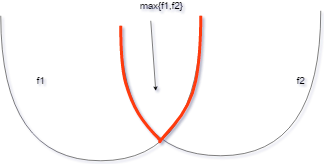
\includegraphics[]{1_3}
\item Composition with linear map.\\
$f \in cvx \R^n$, $A:\R^n \to \R^m$ is a linear map.
$f \circ A (x) = f(Ax) \in cvx \R^n$\\
\begin{align*}
f \circ A (x) & = f(A(\alpha x + (1-\alpha) y)) \\
& = f(A \alpha x + (1-\alpha) A y) \\
& \le \alpha f(Ax) + (a - \alpha) f(Ay)
\end{align*}
\end{itemize}
\chapterimage{intro.jpg} % Chapter heading image
\chapter{Introduzione}\label{1:chintro}

\begin{quote}
e cose di questo tipo\ldots{}
\end{quote}

La Cosmologia è quel ramo della scienza che studia l'universo nel suo
insieme, per comprenderne l'origine e l'evoluzione, mediante strumenti
osservativi, fisici e matematici. In particolare la
cosmologia \emph{planckiana} è si occupa dell'universo nella sua
evoluzione a partire dal tempo di Planck (10\textsuperscript{-43} s). Si
parla di~\emph{evoluzione}~dell'universo da poco più di 100 anni, quindi
è una ``scienza'' giovane. I recenti risultati di Plank offrono le
seguenti stime:~\(\Omega_{M}=0.3, \Omega_{\Lambda}=0.7\) che qui verranno sottintese se non
diversamente indicato. Per quanto riguarda la materia
barionica,~\(\Omega_b=0.05\), ossia il 95\% dell'universo è a noi
sconosciuto. Il modello cosmologico Standard attuale concorda in buona
parte con le osservazioni: quindi~\emph{descrive~}l'universo, ma non è
in grado~\emph{spiegare~}la fisica che ci sta sotto.

Nella prima parte del corso l'universo verrà trattato come un
contenitore di fluido, nella seconda parte verrà trattata la formazione
delle strutture attraverso piccole perturbazioni e instabilità
gravitazionali. I principi del Modello Cosmologico Standard sono due:

\begin{theorem}[Principio Cosmologico]
L'universo (almeno su grande scala) è~\emph{omogeneo} e~\emph{isotropo}.
Oggi per ``grande scala'' si intende circa 100 Mpc, dove l'isotropia è
osservata attraverso la distribuzione delle galassie ad alto z, ma il
concetto di ``grande'' dipende dal tempo cosmico.\label{th:princ1}
\end{theorem}

\begin{theorem}[La Gravità è ben descritta dalla Teoria della Relatività
Generale]
Le proprietà geometriche dello spazio sono legate alla quantità di
energia/materia ivi contenuta. Dal principio precedente ne consegue che
la distribuzione della materia è perfettamente omogenea e isotropa.\label{th:princ2}
\end{theorem}
In passato era in voga il principio cosmologico~\emph{perfetto:}~così
come non esistono direzioni privilegiate, non esistono tempi
privilegiati, ma è stato abbandonato in seguito alla scoperta della
CMB.

\section{Metrica}\label{1:sec1metrica}

È necessaria una metrica per determinare una distanza tra due punti nello spazio-tempo. La definizione più generale affinché omogeneità e isotropia vengano preservate è:
\begin{equation}    
    \mathrm{d}s^2 = g_{\alpha \beta}\, x^\alpha x^\beta
  = g_{00}\mathrm{d}^2t+2g_{0i}\, \mathrm{d}t\mathrm{d}x^i+g_{ij}\mathrm{d}x^i\mathrm{d}x^j \qquad i,j=1,2,3
\end{equation}
dove~\(\alpha,\ \beta=0,\ 1,\ 2,\ 3\)~ e 0 è l'indice della componente temporale del
quadrivettore. Se il valore~\(\mathrm{d}s^2  = 0\) si parla di intervallo di
tipo~\emph{luce~} (la luce viaggia su geodetiche nulle), se è
\textgreater{} 0 di tipo~\emph{tempo}, se è \textless{} 0 di
tipo~\emph{spazio}. Applicando i principi del Modello Standard:
\begin{equation}    
    \mathrm{d}s^2 = c \, \mathrm{d}t^2+g_{ij}\mathrm{d}x^i\mathrm{d}x^j
\end{equation}
ossia~\(g_{0i}=0\) affinché non ci sia una direzione privilegiata
nel tempo (mmm\ldots{}) e~\(g_{00}=c^2\) affinché venga riprodotta
la traiettoria di un fotone.

\par\null

\subsection{Superfici 2D}
Esistono 3 tipi di superfici bidimensionali in base alla curvatura $C$:

\begin{tabular}{l | l | l | l | l}
Superficie & $C$ & Parametrizzazione & .. \\
\hline 
Piano Cartesiano & $0$ & $0\le\rho<\infty$, $0\le\varphi<2\pi$ & $\mathrm{d}l^2=\mathrm{d}\rho^2+\rho^2\mathrm{d}\varphi^2$ & $\rho = ar$ \\
Sup. Sferica & $>0$ & $0\le\theta<\pi$, $0\le\varphi<2\pi$ & $\mathrm{d}l^2=R^2(\sin^2\theta\; \mathrm{d}\varphi^2+\mathrm{d}\theta^2)$ & $R=a, \sin\theta =r $  \\
Sup. Iperbolica & $<0$ & $0\le\theta<\pi$, $0\le\varphi<2\pi$ & $\mathrm{d}l^2=R^2(\sinh^2\theta\; \mathrm{d}\varphi^2+\mathrm{d}\theta^2) $ & $R=a, \sinh\theta =r $ \\
\end{tabular}


Parametrizzandole in coordinate cilindriche è possibile trovare una
forma generale:
\begin{equation}
\mathrm{d}l^2=a^2\left ( r^2\mathrm{d}\varphi^2 + \frac{\mathrm{d}r^2}{1-kr^2}\right); \qquad k=\left\{\begin{matrix}
0 & \textrm{Cartesiano} \\ 
+1 & \textrm{Sferica}  \\
-1 & \textrm{Iperbolica}
\end{matrix}\right.
\end{equation}

\subsection{Superfici 3D}
Analogamente, ponendo~\(\mathrm{d}\Omega^2=\mathrm{d}\theta^2+\sin^2\theta\, \mathrm{d}\varphi^2\), si ricavano le stesse
relazioni per le~ superfici tridimensionali:

\begin{tabular}{l | l | l | l}
Superficie & $C$ & .. \\
\hline
Piano Cartesiano & $0$ & $\mathrm{d}l^2=R^2(\mathrm{d}r^2+r^2\mathrm{d}\Omega^2)$ & $R=a$ \\
Sup. Sferica & $>0$ & $\mathrm{d}l^2=R^2(\mathrm{d}\chi^2+\sin^2\chi\;\mathrm{d}\Omega^2)$ & $R=a, \sin\chi =r $  \\
Sup. Iperbolica & $<0$ & $\mathrm{d}l^2=R^2(\mathrm{d}\chi^2+\sinh^2\chi\;\mathrm{d}\Omega^2)$ & $R=a, \sinh\chi =r $ \\
\end{tabular}
\par\null
Riconducibili alla seguente metrica, detta di~\textbf{Robertson-Walker}
(\textbf{universo omogeneo, isotropo e velocità finita \emph{c} dei
fotoni}):
\par\null

\begin{equation}
\mathrm{d}s^2=c^2\mathrm{d}t^2-a^2\left ( \frac{\mathrm{d}r^2}{1-kr^2} + r^2(\sin^2\theta\;\mathrm{d}^2\varphi+\mathrm{d}^2\theta) \right); \qquad k=\left\{\begin{matrix}
0 & \textrm{Cartesiano} \\ 
+1 & \textrm{Sferica}  \\
-1 & \textrm{Iperbolica}
\end{matrix}\right.
\end{equation}

In precedenza sono state fatte alcune sostituzioni strategiche, si
definiscono quindi:

\begin{itemize}
\item
  \(a\)~~~~\textbf{\emph{fattore di scala (o di
  espansione)}}, che ha dimensioni di una lunghezza (la dimensionalità è
  contenuta esclusivamente in questo parametro) e può dipendete dal
  tempo (\(a=a\left(t\right)\))
\item
  \(k\)~ ~~\textbf{\emph{costante di curvatura}}
\end{itemize}


\section{Distanze}\label{1:sec2distanze}

Esistono diverse definizioni di `distanza', che può dipendere~

\subsection{Distanza Propria}
Si assume di fare una misura istantanea (\(\mathrm{d}t=0\)) della
distanza tra sorgente e osservatore (non è possibile in relatività).
Inoltre si può assumere~ \(\mathrm{d}\theta=\mathrm{d}\varphi=0\) senza perdere di generalità,
ossia ci si pone sulla traiettoria di un fotone che segue le (????).~

\begin{equation}
    d_{PR}=\int_{0}^{r}\frac{a\,\mathrm{d}r'}{\sqrt{1-kr^{'2}}}=a\; \mathfrak{f}(r) \qquad \mathfrak{f}(r):=\left\{\begin{matrix}
\arcsin r& k=+1\\ 
r & k=0\\ 
\mathrm{arcsinh}\:  r & k=-1
\end{matrix}\right.
\end{equation}

Se~\(a=a\left(t\right)\), allora~\(d_{PR}=d_{PR}(t)\) e si può derivare la
velocità:

\begin{align*}
v_R & =\frac{\mathrm{d}d_{PR}}{\mathrm{d}t}=\frac{\dot{a}}{a}d_{PR}=\textrm{H}\,d_{PR}  \\
\textrm{H} & :=\frac{\dot{a}}{a}\quad [\mathrm{s^{-1}}]
\end{align*}

In base a questa relazione, detta~\textbf{legge di Hubble-Lemaitre},
esiste una velocità di recessione nella direzione radiale che è
proporzionale alla distanza. Il~\textbf{parametro di
Hubble}~\(\textrm{H}\), che può dipendere dal tempo, quantifica
questa proporzionalità. Si parla~ambiguamente di~\emph{costante di
Hubble~}riferendosi al fatto che,~\emph{oggi} in~\emph{ogni punto}
dell'universo, possiede lo stesso valore~\(\textrm{H}_0\). Facendone
l'inverso si ottiene il tempo di Hubble, ossia l'età che l'universo
avrebbe se si fosse espanso linearmente.

Si può verificare che la legge di Hubble è già implicita nel principio
cosmologico, ma questo non ci compete.


\begin{definition}[Wong et al., 2019]
Combines time delay data from 6 
quasars to get~\textbf{H}\textsubscript{\textbf{0}} \textbf{= 73.3 $\pm$
1.75{~}km/sec/Mpc}, in agreement with the SH0ES Cepheid-based distance
ladder measurement (\textbf{74.03 $\pm$ 1.42}) and disagreeing with the
latest CMB model based value, \textbf{H}\textsubscript{\textbf{0}}
\textbf{= 67.80 $\pm$ 0.9 km/sec/Mpc}. On the other hand Freedman et al. get
a distance ladder value of \textbf{H}\textsubscript{\textbf{0}}
\textbf{= 69.8 $\pm$ 0.8 (stat) $\pm$ 1.7 (syst) km/sec/Mpc} using the tip of
the red giant branch to calibrate Type Ia supernovae.
\vspace*{0.5em}

From: Ned Wright's Website
\end{definition}

La \emph{Distanza Propria} calcolata ad \emph{oggi} è definita
\textbf{Distanza Comovente (o Comobile)}:

\begin{equation}
d_{C}:=d_{PR}(t=t_0)=a(t_0)\mathfrak{f}(r)=\frac{a(t_0)}{a(t)}d_{PR}
\end{equation}

\subsection{Redshift}

Siano~\(\lambda_e\) la lunghezza d'onda di un segnale emesso
localmente da una sorgente e~\(\lambda_{ob}\) quella ricevuta
dall'osservatore si definisce~\emph{redshift} la quantità

\begin{equation}
z=\frac{\lambda_{ob}-\lambda_e}{\lambda_e}=\frac{\lambda_{ob}}{\lambda_e}-1
\end{equation}

Si cosideri l'emissione consecutiva di due fotoni a~~\(t_e\)
e~\(t_e+\delta\ t_e\) rispettivamente. Come già visto in precedenza si
ha~\(\mathrm{d}s^2=0\) e si può assumere~\(\mathrm{d}\theta=\mathrm{d}\varphi=0\) senza perdere
di generalità. Dall'equazione (4) si ottiene:

\begin{equation}
\int_{t_{e}}^{t_{ob}}\frac{c\,\mathrm{d}t}{a(t)}=\int_{0}^{r}\frac{\mathrm{d}r'}{\sqrt{1-kr'}}=\mathfrak{f}(r)\equiv \int_{t_{e}+\delta t_e}^{t_{ob}+\delta t_{ob}}\frac{c\,\mathrm{d}t}{a(t)}
\end{equation}

dal momento che~\(\mathfrak{f}(r)\) dipende solo dalla geometria.
Per~\(\delta t_{e}\) e~\(\delta t_{ob}\) piccoli
(ossia~\(a=cost\) ne tempo di integrazione),
ponendo~\(a_e=a\) e~\(a_{ob}=a_0\) (0, \emph{oggi}), si
ottengono le seguenti relazioni:

\begin{equation}
\frac{\delta t_0}{a_0}=\frac{\delta t_e}{a};\qquad a\nu_e=a_0\nu_0;\qquad 1+z=\frac{a_0}{a}
\end{equation}

Possiamo quindi pensare~\(z\) come la misura di quanto è
variato il fattore di scala dal tempo dell'emissione del fotone. Un
risultato analogo poteva essere ottenuto ipotizzando osservatore e
sorgente in moto relativo (effetto Doppler), ma non esiste una velocità
effettiva di allontanamento: è lo spazio che si dilata.


\subsection{Distanza di Luminosità}

Si definisce a partire dalla relazione tra luminosità~\(L [erg/s]\)
e flusso~\(l\) considerando i seguenti effetti:

\begin{itemize}
\item
  \emph{Dilatazione temporale:~\(\frac{\mathrm{d}t}{\mathrm{d}t_0}=\frac{a(t)}{a(t_0)}\)}
\item
  \emph{Redshift (cambiamento di energia)}:~\(\frac{\varepsilon_0}{\varepsilon}=\frac{a(t)}{a(t_0)}\)
\end{itemize}

\begin{itemize}
\item
  \emph{Variazione della geodetica:~\(r\rightarrow ar\)}
\end{itemize}

\par\null

\begin{equation}
l=\frac{L}{4\pi d_L^2}=\frac{L}{4\pi a_0^2r^2}\frac{a^2}{a_0^2}=\frac{L}{4\pi a_0^2r^2}\frac{1}{(1+z)^2}\qquad d_L := a_0 r (1+z)
\end{equation}

\subsubsection*{Distanza (di diametro)
Angolare}

{\label{564376}}

Si definisce misurando le dimensioni angolari di un righello standard,
ossia di una classe di oggetti astrofisici che hanno la stessa
dimensione intrinseca~\(D\) posti a distanza diversa (in
realtà non esistono,~\emph{sigh}). Si parte dall'equazione (3) e si
assume~\(\mathrm{d}r=\mathrm{d}\varphi = 0\) e~\(\mathrm{d}t=0\) (poichè si osservano le
due estremità dell'oggetto contemporaneamente):

\par\null

\begin{equation}
(D^2=)\, \mathrm{d}s^2=a^2r^2\mathrm{d}\theta^2\rightarrow \frac{D}{\mathrm{d}\theta}=ar\qquad d_A:=a(t)\, r
\end{equation}

Confrontandola con la (12) si ottiene la~\textbf{relazione di dualità}:

\begin{equation}
d_A=\frac{d_L}{(1+z)^2}
\end{equation}

Queste due distanze sono definite diversamente, non ce ne è un ``più
fisica'' dell'altra: la scelta va fatta in base al tipo di osservazione.
Se si utilizza la luminosità intrinseca (es. cefeidi, SNe, \ldots{}) per
stimare la distanza, si applica la definizione~\(\mathrm{d}_L\); se
esistesse un righello standard cosmologico (es. orizzonte cosmologico),
si applica la definizione~\(\mathrm{d}_A\). Questa relazione DEVE
valer se l'universo fosse Robertson-Walker, mentre in un universo
statico si avrebbe~\(d_A=d_L\).~

Esistono altre definizioni di distanza: parallasse, moti propri e così
via\ldots{} Tutte tendono allo stesso valore per \(z\)
piccoli.

\par\null

Sommario:

\begin{align*}
d_{PR} & =a\,\mathfrak{f}(r)  \\ 
d_{C} & =\frac{a_0}{a}\,\mathrm{d}_{PR}  \\ 
d_L & = a_0 \, r\, (1+z)  \\ 
d_A & =a\, r  \\
1+z & =\frac{a_0}{a}
\end{align*}

\par\null

\subsection{Risultati Osservativi}

Tutte le distanze possono essere riscritte in funzione di un unico
parametro $a=a(t)$ sviluppandolo in serie:
\begin{equation}
a(t)\simeq a_0\left ( 1+H_0 (t-t_0)-\frac{1}{2}q_0\,H_0^2(t-t_0)^2  \right )\qquad 
H:=\frac{\dot{a}}{a}; \quad
q:=-\frac{\ddot{a} a}{\dot{a}^2} 
\end{equation}

dove $q$ è detto \emph{parametro di decelerazione} ed è adimensionale. Viene definito col - perché in passato i modelli sostenevano che l'espansione dell'universo fosse decelerata. 

\subsubsection{Hubble test applicato a $d_L$}
Applicando lo sviluppo alla \emph{distanza di luminosità} si ha:

\begin{equation}
d_L\simeq \frac{cz}{H_0}\left ( 1 + \frac{1}{2}(1-q_0)z  \right )
\end{equation}

da cui, applicando il logaritmo e sviluppando per \(\log\left(1+x\right)\rightarrow\ \frac{x}{\ln10}\), si
ottiene la relazione:

\begin{equation}
\log d_L = \log cz-\log H_0+0.217(1-q_0)z;
\end{equation}

oppure, esplicitandola in magnitudini ($ m-M=\mu=5\log\frac{d}{\mathrm{10\,pc}} $):

\begin{equation}
\underline{m} - \underbrace{M} = 25 + 5\log c\underline{z}-5\log H_0 + 1.086~(1-q_0)~\underline{z};
\end{equation}

dalla quale tramite $\textrm{\underline{osservazioni}}$ e $\underbrace{\textrm{modelli}} $ (es. per le SNTN $M_V=-19$ è possibile calibrare $H_0$ localmente e $q_0$ a $z$ più elevato.

\subsubsection{Hubble test applicato alla densità di oggetti}
In un universo euclideo si ha che la densità di oggetti $N\propto d_L^3$. Tutti gli oggetti con flusso superiore ad $l$ saranno contenuti in un cubo di densità $N(<l)\propto l^{-\frac{3}{2}}$. Quindi si dovrà osservare la relazione: 
\begin{equation}
\log N(>l) \propto -1.5 \log l \propto 0.6~m;
\end{equation}

Rilassando il vincolo di universo euclideo è necessario calcolare l'integrale:
\begin{equation}
N(l)= 4\pi \int_{0}^{r}\mathrm{d}r'\frac{r'^2}{\sqrt{1-kr'^2}}~n(t(r'))~a(t(r'))^3;
\end{equation}
che si risolve assumendo che esista una classe di oggetti celesti per la quale la densità rimane costante nel tempo ($n_0a_0^3=na^3$). In passato le prime stime furono fatte mediante le galassie, oggi sappiamo che non esistono oggetti che si comportano così per tempi cosmologici.
In questa assunzione si può espandere la funzione integranda $\frac{r'^2}{\sqrt{1-kr'^2}}$ per $r\rightarrow 0$ per ottenere la relazione:
\begin{equation}
\log N(>l) = cost + 3\log z - \frac{3}{2\ln 10}~(1+q_0)~z;
\end{equation}
in cui $H_0$ è in pancia alla $cost$. Si noti che il numero di oggetti non diverge (cfr. Paradosso di Olbers), ci arriva informazione solo da una parte di Universo, quello in connessione causale con noi.



\chapterimage{head2.png} % Chapter heading image
\chapter{Universi di Friedmann}\label{2:chuniinfuga}

\section{Equazioni di Friedmann}
I modelli di Friedmann prevedono 3 ingredienti:
\begin{itemize}
    \item Teoria della Relatività Generale (eq. di Einstein)
    \item Universo Omogeneo e Isotropo
    \item Fluido Perfetto
\end{itemize}


Le equazioni di campo di Einstein sono un set di 16 equazioni che descrivono l'interazione gravitazionale come il risultato dell' spazio-tempo curvato da massa ed energia. 
$$R_{\mu \nu} - \frac{1}{2} R \, g_{\mu \nu} = \frac{8 \pi G}{c^4} T_{\mu \nu}.$$

Il membro di sinistra rappresenta la parte geometrica, mediante il tensore di Ricci $R_{\mu \nu}$, il tensore geometrico $g_{\mu \nu}$ e lo scalare di Ricci $R$. Il membro di destra rappresenta il contenuto di energia-materi dell'universo tramite il tensore energia-impulso $_{\mu \nu}$. 
Nei modelli di Friedmann che prevedono omogeneità e isotropia, il tensore metrico $g_{\mu \nu}$ è descritto dalla metrica di Robertson Walker. Inoltre, assumendo la condizione di fluido perfetto (no viscosità, no conduzione), il tensore energia-impulso dipende esclusivamente da pressione $p$ e densità $\rho$:
$$T_{\mu \nu}=-pg_{\mu \nu}+(p+\rho c^2)u_\mu u_\nu .$$

Delle 16 equazioni soltanto 2 non diventano delle identità e sono quelle tempo-tempo e spazio-spazio:
$$
\ddot{a}=-\frac{4\pi}{3}G\left ( \rho+\frac{3p}{c^2} \right )a\quad (tempo); \qquad
a\ddot{a}+2\dot{a}^2+2kc^2=4\pi G \left ( \rho - \frac{p}{c^2} \right )a^2\quad (spazio).
$$
Per ricavarle ci vorrebbe una settimana di lezioni e calcoli per ottenere tramite la metrica tutti i simboli di Christoffel. Verranno ricavate in approssimazione newtoniana. In ogni caso si sostituisce $\ddot{a}$ della prima equazione nella seconda e si ottengono la \textbf{Prima e Seconda Equazione di Friedmann}.

\begin{align}
   & \ddot{a}  =-\frac{4\pi}{3}G\left ( \rho+\frac{3p}{c^2} \right )a \label{eq:friedmann1}\\
   & \dot{a}^2+kc^2  =\frac{8\pi}{3}G\rho a^2 \label{eq:friedmann2}
\end{align}

Che possono essere legate tra loro dall'equazione di adiabaticità (perché l'universo non dovrebbe essere adiabatico?) nella forma $\mathrm{d}\mathfrak{U}=-p\mathrm{d}\mathfrak{V}$ ossia:

\begin{equation}
    \mathrm{d}(\rho c^2 a^3)=-p\mathrm{d}a^3
\end{equation}
Soltanto 2 di queste 3 equazioni sono comunque indipendenti tra di loro.

\vspace*{1em}
Proviamo a giustificarle in ambito newtoniano studiando $a$ in funzione del tempo e utilizzando i due teoremi di Birkoff che sono gli equivalenti del teorema di Gauss in relatività generale.
\begin{theorem}[Teoremi di Birkoff]
(1) Il campo gravitazionale di un corpo sferico in una spazio vuoto è statico ed è descritto al suo esterno dalla metrica di Scwartzchild (quella di un oggetto puntiforme).

(2) Il campo gravitazionale prodotto da un guscio sferico (anche non statico) è descritto al suo interno dalla metrica di Minkowski (quella dello spazio piatto).
\end{theorem}

Si studia la dinamica di un punto $P$ posto su una sfera di raggio $l=d_C \frac{a}{a_0}=:\tilde{D}a$ centrata in $O$. Affinché si possano trascurare gli effetti relativistici, il tempo di collasso libera $\tau_{ff}\propto (G\rho)^{-1/2}$ deve essere molto maggiore del \textit{light crossing time} $\tau =l / c$. Parimenti, si possono considerare scale più grande del raggio di Schwarzchild (scala su cui l'energia di massa è in equilibrio con quella gravitazionale). Dall'equazione del moto di Newton si ha:
$$
\dot{l}\:\frac{\mathrm{d^2} l}{\mathrm{d} t^2}=\frac{Gm}{l^2}\dot{l} \quad \rightarrow \quad \frac{\mathrm{d} }{\mathrm{d} t}\left ( \frac{\dot{l}^2}{2} \right )=\frac{\mathrm{d} }{\mathrm{d} t}\left ( \frac{GM}{l} \right ) \quad \rightarrow \quad \dot{a}^2 =\frac{8\pi}{3}G\rho a^2+cost
$$
Si può ottenere la seconda equazione di Friedmann se si assume $cost=-kc^2$. Questa non è altro che l'equazione di conservazione dell'energia, per la quale $-kc^2$ rappresenta la somma dei contributi di energia cinetica e potenziale. Per $k=0$ si ha un bilanciamente perfetto, per $k=+1$ domina il termine potenziale (collasso) e per $k=-1$ domina il termine cinetico (espansione).

La prima equazione di Friedmann si ricava in maniera analoga utilizzando un trucchetto relativistico $\rho_{eff}=\rho+\frac{3p}{c^2}$, ossia esiste una densità effettiva data dalla densità di massa e da un termine relativistico legato alla pressione. L'equazione si ricava passando dalla massa alla densità e utilizzando la densità effettiva.
Si può dimostrare, per verificare che si è ancora in grado di fare i conti, che utilizzando l'equazione di adiabaticità si ottiene anche la seconda equazione di Friedmann.


In passato l'idea generale era che l'universo dovesse essere statico, ma le relazioni (\ref{eq:friedmann1} e \ref{eq:friedmann2}) prevedono un universo in espansione. Sarebbe pertanto necessario porre $\rho + 3p/c^2 = 0$, se non fosse che questa condizione è \textit{unphysical} dato che pressione e densità dovrebbero avere un segno discorde. Per cui...
\begin{definition}[Einstein:]
«Grazie mille Sig. Friedmann, ho capito che c'è qualcosa che non va nelle mie equazioni». Senza Fonte.
\end{definition}
... Einstein, nel 1921, introdusse il termine $- \Lambda g_{\mu \nu}$ [L$^2$]:

$$R_{\mu \nu} - \frac{1}{2} R \, g_{\mu \nu} - \Lambda g_{\mu \nu}= \frac{8 \pi G}{c^4} T_{\mu \nu}.$$

Ancora oggi non è chiaro se il termine $- \Lambda g_{\mu \nu}$ sia legato alla geometria dello spazio-tempo come sosteneva Einstein (teoria della gravità modificata) o alla parte energetica (energia oscura, noi votiamo per lei).  
Il tensore energia-impulso viene modificato in: $\tilde{T_{\mu \nu}}=T_{\mu \nu}+\Lambda g_{\mu \nu}\frac{\Lambda c^4}{8 \pi G}$. Lambda contribuisce in modo negativo alla pressione e positivo alla densità e le equazioni di Friedmann diventano:
\begin{align}
   & \ddot{a}  =-\frac{4\pi}{3}G\left ( \tilde{\rho}+\frac{3\tilde{p}}{c^2} \right )a & \tilde{p}=p + p_\Lambda = p - \frac{\Lambda c^4}{8 \pi G}  \label{eq:friedmann1tilde} \\
   & \dot{a}^2+kc^2  =\frac{8\pi}{3}G\tilde{\rho} a^2 & \tilde{\rho}=\rho + \rho_\Lambda = \rho + \frac{\Lambda c^2}{8 \pi G} \label{eq:friedmann2tilde}
\end{align}


\subsection{Modello di Einstein}
Il modello di Einstein soddisfa le seguenti richieste: 
\begin{itemize}
    \item $\dot{a}=\ddot{a}=0$
    \item Universo di sola materia con $p=p_b=0$
\end{itemize}
Applicando questi vincoli alle equazioni di Friedmann (\ref{eq:friedmann1}) e utilizzando le definizioni di $\tilde{\rho}$ e $\tilde{p} $ si ottiene:
$$
\tilde{p}= -\frac{\Lambda c^4}{8 \pi G}\quad \mathrm{e}\quad \tilde{p} = - \frac{k c^4}{8 \pi G a^2} \qquad  \Rightarrow \qquad \Lambda=\frac{k}{a^2}\quad \mathrm{[L^{-2}]}
$$
che mostra come, nel modello di Einstein, $\Lambda$ sia legata al parametro di curvatura. Inoltre si può calcolare qual è la densità ordinaria $\rho$:
$$
\rho = \tilde{\rho} - \rho_\Lambda = \frac{3 k c^2}{8 \pi G a^2} - \frac{k c^2}{8 \pi G a^2}=\frac{k c^2}{4 \pi G a^2}
$$
Questo valore, per avere senso fisicamente, deve essere positivo ossia si deve verificare che $k=+1$.
Infine si può calcolare qual è il valore di $\Lambda$ che rende l'universo statico:
$$
\Lambda_e = \frac{4\pi G\rho}{c^2}
$$
Quindi quello di Einstein è un universo di materia con \textbf{geometria sferica} e diventa statico allorché $\Lambda =\Lambda_e$. 

Per soddisfare il pregiudizio dell'epoca (universo eterno e statico) si è complicato l'equazione in modo arbitrario (pur conservando linearità, ...) e ha dovuto inserire una richiesta cavillosa (la cosmologica deve avere un valore ben preciso). Nel 1929 Hubble scoprì l'espansione dell'universo, Einstein prese una penna e scancellò la $\Lambda$.

\subsection{Modello di De Sitter}
Il modello di De Sitter, seppur stravagante, tornerà utile più avanti per modellare il periodo dell'inflazione. Si basa sulle seguenti assunzioni:
\begin{itemize}
    \item Universo completamente vuoto di materia: $\rho=0$ e $p=0$;
    \item Universo piatto: $k=0$;
    \item L'unico contributo è quello della $\Lambda\neq 0$.
\end{itemize}
Tramite le definizioni di $\tilde{\rho}$ e $\tilde{p} $ si ottiene:
$$
\tilde{p}=-\tilde{\rho}c^2
$$
Ritroveremo queste equazione per la descrizione del vuoto (interpretazione moderna della costante cosmologica). Utilizzando la prima equazione di Friedmann \ref{eq:friedmann1} e la definizione $\rho_\Lambda$ si ottiene:
\begin{equation}
    a = a_0~e^{H\, \mathrm{d}t}\qquad H=\frac{\dot{a}}{a}=\sqrt{\frac{\Lambda}{3}}c= cost
\end{equation}
Quindi quello di De Sitter è un universo privo di materia con geometria piatta che evolve con accelerazione esponenziale per un tempo infinito. 

Non esiste un principio fisico che afferma che l'energia del vuoto sia 0. Ogni qual volta si è trovato un problema nel Modello Standard, si è trovato la soluzione aggiungendo la costante cosmologica (con un parametro in più i dati fittano meglio). Come negli anni '60 in cui si è scoperto un eccesso di quasar a $z=2$, giustificato da Lemaitre tramite la reintroduzione $\Lambda$.
\vspace*{0.5em}

\begin{definition}
    The 1960s also saw the discovery of puzzling new astronomical entities, extremely luminous
objects apparently lying at tremendous distance (Schmidt 1963, 1965: Schmidt and Matthews
1964; Sandage 1965). Two unusual aspects of the entities (soon known as quasi-stellar
objects or ‘quasars’) were that they did not appear to conform to the standard relation
between redshift and distance obeyed by ordinary galaxies, while they exhibited a
preponderance of redshifts at around the large value of z = 2 (Hoyle and Burbidge 1966;
Longair and Scheuer 1967; Burbidge and Burbidge 1967). The discovery prompted a new
appraisal of Lemaître’s hesitating model of the cosmos, with a number of
physicists interpreting the phenomenon as evidence for a stagnant phase in cosmic expansion
due to a positive cosmological constant.
Lemaître proposed his famous hypothesis of a universe that originated as a ‘primeval atom’ (Lemaître
1931b; Kragh and Lambert 2007). With such cosmic origins in mind, he noted that a
judicious choice of value for the cosmological constant could give a cosmic expansion in
three stages; an initial phase during which the expansion is de-accelerated by gravity, a
‘loitering’ phase in which the de-acceleration is balanced by the repulsive influence of the
cosmic constant, and a final phase in which the repulsion becomes dominant (Lemaître
1931c, 1931d, 1933). Here the cosmic expansion was governed by a cosmological constant
given $\Lambda=\Lambda_e (1+\varepsilon)$ where the adjustable parameter $\varepsilon$ determined the length of the stagnation period. A schematic of this model, known as the ‘hesitating’ or ‘loitering’ universe is shown below.

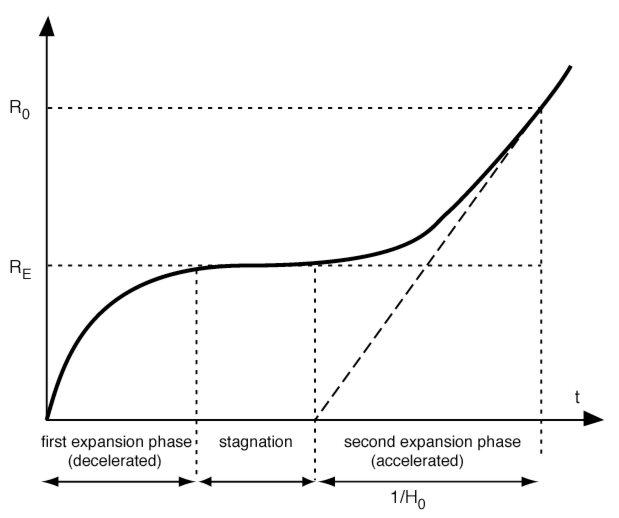
\includegraphics[width=.6\textwidth]{Pictures/2/Uhesitating.png}
\vspace*{0.5em}

From: cita O'Raif \& Luminet 2011
\end{definition}
\vspace*{0.5em}
In realtà si è scoperto che avere i quasar a $z=2$ era un effetto dovuto a bias di selezione e la costante cosmologica è stata nuovamente messa da parte. Infine negli anni '70 si è osservato tramite le SNe che l'espansione dell'universo oggi è accelerata e ciò è giustificabile con una costante cosmologica che rende $\ddot{a}>0$ (contribuendo negativamente alla pressione).


\section{Soluzioni analitiche del Modello di Friedmann}
\subsection{Parametro di Densità e Geometria}
Manipolando le equazioni di Friedmann è possibile introdurre numerosi parametri strategici per studiare i legami tra le variabili fondamentali della cosmologia.

\begin{align*}
   & \ddot{a}  =-\frac{4\pi}{3}G\left ( \tilde{\rho}+\frac{3\tilde{p}}{c^2} \right )a &  H:=\frac{\dot{a}}{\dot{a}} \\
      & \dot{a}^2+kc^2  =\frac{8\pi}{3}G\tilde{\rho} a^2 & q:= - \frac{\ddot{a}a}{\dot{a}^2} \\
   & \mathrm{d}(\rho c^2 a^3)= - p \mathrm{d}a^3 & \rho_{cr}:=\frac{3H^2}{8 \pi G}
\end{align*}

Dividendo la seconda equazione per $a_0^2$ e inserendo i parametri $H_0$ e $\rho_0$ si ottiene:
\begin{equation}
    H_0^2 \left ( 1-\frac{\rho_0}{\rho_{cr,0}}  \right ) = -\frac{kc^2}{a_0^2} \label{eq:friedmannh0rho0}
\end{equation}

Il segno di $k$ è determinato dall'anti-segno della parentesi tonda. Si definisce \textbf{parametro di densità} il valore:
\begin{equation}
    \Omega=\frac{\rho}{\rho_{cr}}\qquad\quad \Omega_0 \left\{\begin{matrix}
=1 & \rho_0=\rho_{cr,0} & k=0 & piatto\\ 
>1 & \rho_0>\rho_{cr,0} & k=+1 & sferico\\ 
<1 & \rho_0<\rho_{cr,0} & k=-1 & iperbolico
\end{matrix}\right.
\end{equation}
Affinché l'universo sia piatto e non curvo, il parametro di densità deve avere un valore estremamente preciso (per questo motivo è detta densità \textit{critica}).

Le misure ci dicono che:
\begin{align}
    \rho_{cr,0} & \simeq 1.9\cdot 10^{-29}h^2\quad [\mathrm{g\;cm^{-3}}] \\
    & \simeq 2.775\cdot 10^{11}h^2\quad [\mathrm{M_\odot\;Mpc^{-3}}]
\end{align}

Per determinare la geometria dell'universo bisogna conoscere $\Omega_0$, misurando la densità oggi e confrontandola con quella critica. Nel calcolo della densità vanno considerate tutte le componenti.
Nell'universo attuale materia ed energia oscura dominano, possiamo descrivere l'universo come fluido costituito da due componenti. Per far ciò si utilizzano le definizioni di $\tilde{\rho}$ e $\tilde{p}$ nell'equazione di Friedmann:
$$
\ddot{a}  =-\frac{4\pi}{3}G\left ( \rho+\frac{3p}{c^2} \right ) a + \frac{\Lambda c^2}{3}a
$$
Grazie al secondo termine si potrebbe avere un'accelerazione positiva.
Dividendo l'altra equazione per $a_0^2$  si ha:
\begin{equation}
    H_0^2 \left ( 1-\frac{\rho_0}{\rho_{cr,0}} -\frac{\rho_{0,\Lambda}}{\rho_{cr,0}} \right ) = -\frac{kc^2}{a_0^2}
\end{equation}
da cui introducendo il parametro di densità totale:
\begin{equation}
    H_0^2 \left ( 1-\Omega_{TOT} \right ) = -\frac{kc^2}{a_0^2}\qquad \Omega_{TOT}=\Omega_{0}+\Omega_{0\Lambda}
\end{equation}
La curvatura è ora definita da quanto dal somma delle due componenti differisce dall'unità (ocio: $\Omega_0 = \Omega_{0m}$ ossia in questo caso $\Omega_0$ è riferito alla materia). 


\subsection{Equazione di Stato}
L'Universo è costituito da 3 principali componenti:

\begin{example}[Materia non relativistica]
$p_m=nk_B T = \frac{\rho_m}{m_p}k_B T \approx 0 \qquad ( \rho_m \approx 0) $
\end{example}
\begin{example}[Radiazione o Materia relativistica]
$p_R=\frac{1}{3} \rho_R c^2 $
\end{example}
\begin{example}[Costante Cosmologica]
$p_\Lambda= -\rho_\Lambda c^2 $
\end{example}

In cosmologia si definisce quindi il termine $w$ per l'equazione di stato:
\begin{equation}
    p=w\rho c^2\quad\rightarrow \quad c_s^2=\left ( \frac{\partial p}{\partial \rho}\right )_{S}=wc^2 \qquad \quad w= \left\{\begin{matrix}
0& materia\\
1/3 & comp. radiativa\\
-1 & cost. cosm
\end{matrix}\right.
\end{equation}
Affinché la velocità del suono $c_s$ rimanga minore di quella della luce $c$, bisogna che $w<1 $ (a $w=1 $ si ha quella conosciuta come \textit{stiff matter}). Inoltre, la positività della pressione nella fisica ordinaria richiede $w>0 $. Quindi il \textbf{parametro dell'equazione di stato} $w $ nella fisica ordinaria può assumere un valore $0<w\leq 1$ (intervallo di Zeldovich).

Armati di questo, lo si applica all'equazione di adiabaticità, si sviluppa il differenziale e si integra per separazione di variabili:
\begin{equation}
    \rho=\rho_0 \left ( \frac{a}{a_0}\right )^{-3(1+w)}\qquad\rightarrow \qquad \rho \propto z^\alpha =\qquad \alpha
\left\{\begin{matrix}
3 & materia\\
4 & comp. radiativa\\
0 & cost. cosm
\end{matrix}\right.
\label{eq:rhoaw} \end{equation}
Gli esponenti non ci sorprendono: $a^{-3}$ nel caso della materia è come dire $Vol^{-1}$, nel caso della componente relativistica si aggiunge un altro $a^{-1}$ dovuto al redshift.

\begin{figure}[h]
    \centering
    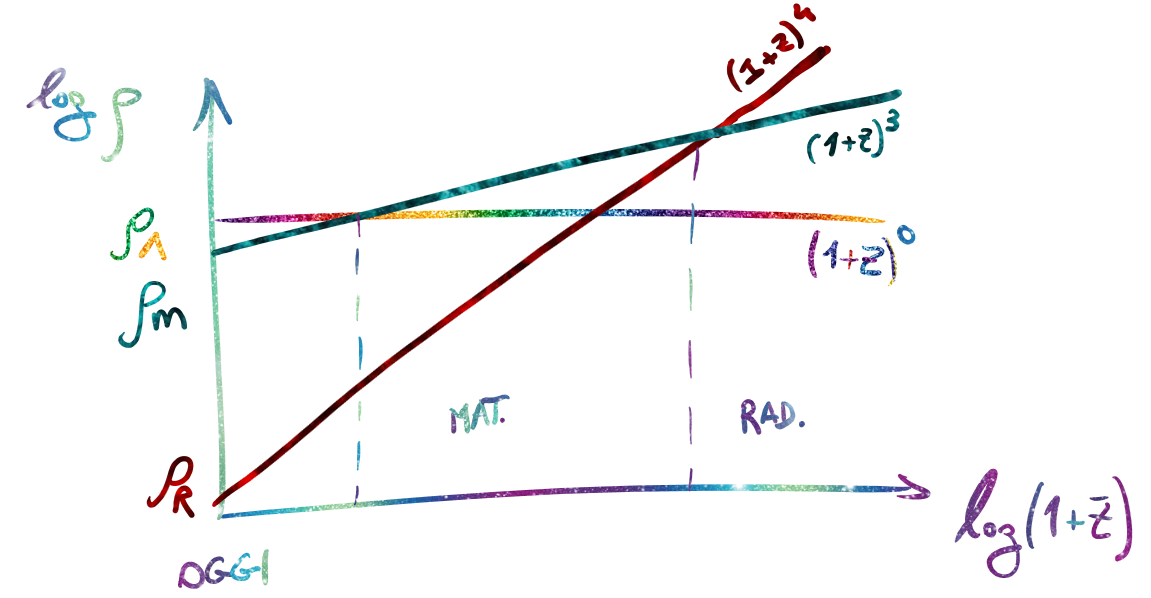
\includegraphics[width=.8\textwidth]{Pictures/2/logrho-z.png}
    \caption{Andamento della densità delle tre componenti al variare del redshift.}
    \label{fig:2rhored}
\end{figure}
Sostituendo il valore della densità della (2.14) nell'equazione di Friedmann e facendo qualche operazione cosmatematica si ottiene:
\begin{equation}
    H^2=H_0^2\,(1+z)^2\left [ 1-\Omega_0 + \Omega_0 \,(1+z)^{1+3w} \right ] \label{eq:hevol}
\end{equation}
che regola l'evoluzione del tempo del parametro di Hubble (la geometria è in $\Omega_0$). In universo con più componenti assume la forma generale:
\begin{equation}
    H^2=H_0^2\,(1+z)^2\left [ 1-\sum_{i}\Omega_{0i} + \sum_{i}\Omega_{0i} \,(1+z)^{1+3w_i} \right ] = H_0^2\: E(z)^2 \label{eq:hevolmulti}
\end{equation}
Per l'universo attuale bisogna includere $\Omega_m$ e $\Omega_\Lambda$. 

Si assume ora che ci sia una sola componente, la materia, per cui $0\leq w \leq 1$. Della prima equazione di Friedmann, $\ddot{a}$ restituisce necessariamente un valore strettamente negativo, ossia la funzione $a(t)$ ha la concavità verso il basso e non può avere un flesso. Inoltre sappiamo osservativamente che l'universo è in espansione $\dot{a}_0>0$. La funzione $a(t)$ è quindi monotona crescente e tornando indietro nel tempo si ha che inevitabilmente interseca l'asse del tempo, ossia esiste un $t=0$ (un inizio del tempo, "Big Bang"). Solo se esistesse un fluido avente $w<-1/3$ si potrebbe avere un flesso.  Il Big Bang è accompagnato da condizioni fisiche antipatiche, ossia per $t\rightarrow 0$ si avrebbe: $a\rightarrow 0$, $\rho \rightarrow \infty$, $T \rightarrow \infty$. Questo è dovuto al fatto che si entra in regimi di cui non si conoscono le leggi fisiche, il limite di validità è il Tempo di Planck $\approx 10^{-43}$ s. Per evitare il Big Bang: universo non omogeneo e isotropo (no RW), fluido non perfetto, componente con $w<-1/3$ (c'è, ma si vedrà che non è sufficiente).

\subsection{Universo di Einstein - De Sitter}
Il modello di Einstein - De Sitter caratterizza un universo piatto $k=0$ ($\Omega_0 =1$). Le soluzioni sono estremamente importanti perché valgono per buona parte dell'universo. Partendo dall'equazione (\ref{eq:hevol}) si ottengono le seguenti relazioni per i parametri principali:
\begin{align}
    & a(t) = a_0 \left ( \frac{t}{t_0} \right )^{\frac{2}{3(1+w)}} \\
    & t = t_0 \left ( 1+z \right )^{\frac{-3(1+w)}{2}} \\
    & H = \frac{2}{3(1+w)}\frac{1}{t}=\frac{H_0 ~t_0}{t}=H_0 (1+z)^{\frac{3(1+w)}{2}} \\
    & q = \frac{1+3w}{2} > 0 \\
    & t_0 = \frac{2}{3(1+w)}\frac{1}{H_0} \\
    & \rho  = \rho_0 \left ( \frac{t}{t_0} \right )^{-2}= \rho_0 \frac{1}{6\pi G (1+w)^2}\frac{1}{t^2}
\end{align}
L'universo è in espansione monotona crescente (ma decelerata in modo costante) ed è infinito. Verso il Big Bang $H\rightarrow \infty$, inoltre all'aumentare di $w$ (pressione) $\ddot{a}$ diventa più basso, fenomeno contrario al concetto di "scoppio"! Infatti il nome "Big Bang" era stato assegnato al modello da coloro che lo sfottevano. Il tempo dell'universo oggi (età) non è esattamente $1/H_0$ per l'effetto della decelerazione dell'espansione.


\begin{table}[h]
\centering
\def\arraystretch{1.5}
\begin{tabular}{@{}ll@{}}
\toprule
\textbf{$w=0$ (materia)} & \textbf{$w=\frac{1}{3}$ (radiazione)} \\ \midrule
$a\propto t^{2/3}$ & $a\propto t^{1/2}$ \\
$t = t_0 \left ( 1+z \right )^{-3/2}$ & $t = t_0 \left ( 1+z \right )^{-2}$ \\
$H = H_0 (1+z)^{3/2} = \frac{2}{3t} $ & $H = H_0 (1+z)^{2} = \frac{1}{2t}$ \\
$q =1/2 $ & $q = 1$ \\
$t_0 = \frac{2}{3}\frac{1}{H_0}$ & $t_0 = \frac{1}{2}\frac{1}{H_0}$ \\
$\rho  = \rho_0 \frac{1}{6\pi G}\frac{1}{t^2}$ & $\rho  =  \rho_0 \frac{3}{32\pi G}\frac{1}{t^2}$ \\ \bottomrule
\end{tabular}
\end{table}

\subsection{Universi Curvi}
Per analizzare il comportamento dei principali parametri cosmologici nel caso di universi non piatti, si modifica l'equazione (\ref{eq:hevol}) come segue:
$$
\left ( \frac{\dot{a}}{a_0} \right )^2 = H_0^2 \left [ (1-\Omega_0 ) + \Omega_0 \left ( \frac{a_0}{a} \right )^{1+3w} \right ]
$$
Il primo termine nella parentesi quadra, il termine di curvatura, è costante. Il secondo dipende dal tempo, quindi si studia per quale valore di $a$ i due si equivalgono:
$$
a^*:\quad \left | 1-\Omega_0  \right | = \Omega_0\left ( \frac{a_0}{a^*} \right )^{1+3w}\qquad \leftrightarrow \qquad z^*:\quad \left | \Omega_0^{-1} - 1  \right |^{\frac{1}{1+3w}}
$$
Quando $a\ll a^*$ oppure $z\gg z^*$ (vicino al Big Bang), l'equazione diventa:
$$
\dot{a}=a_0~ H_0 ~\Omega_0^{1/2} \left ( \frac{a_0}{a}\right )^{\frac{1+3w}{2}}
$$
un fattore costante $\Omega_0^{1/2}$ in più rispetto al modello Einstein De Sitter, ossia tutti gli universi curvi si comportano come quello piatto vicino al Big Bang. Un'eventuale curvatura diventerebbe significativa a  $\left |  1+z^* \right | =  \left | \Omega_0^{-1} - 1  \right |$. Per esempio, $z^* =10$ per $\Omega_0=0.1$ e $z^* = 2$ per $\Omega_0=0.3$.

\begin{theorem}[Messaggio]
Anche se fosse curvo, possiamo assumere l'universo piatto per buona parte della sua storia (almeno fino a $z\approx 10$). Per studiare l'eventuale curvatura è necessario fare osservazioni vicine a oggi.
\end{theorem}

Quando $a\gg a^*$ oppure $z\ll z^*$, si distinguono quindi i due casi

\subsubsection{Universi Aperti}
In questo caso $\Omega_0 < 1$, quindi $\dot{a}$ è strettamente positiva. Dato che osservativamente $\dot{a}_0 >0$, l'espansione è monotona crescente e vale:
\begin{align}
   & \dot{a}=a_0~ H_0 ~ \sqrt{1-\Omega_0 }=cost \\
   & a=a_0~ H_0 ~ \sqrt{1-\Omega_0 }~ t  \propto t \\
   & H= 1/t \\
   & q= 0 \\
   & \rho =\rho_{cr} ~\Omega_0 \left ( H_0  ~(1-\Omega_0)^{1/2} ~ t   \right )^{-3(1+w)}
\end{align}
In particolare si ha un'espansione lineare libera (non decelerata con nel modello EdS), quindi $a$ cresce più velocemente. 

\subsubsection{Universi Chiusi}
In questo caso $\Omega_0 > 1$, quindi può esistere un valore di $a$ per cui $\dot{a}=0$ , ossia la crescita dell'universo si arresta. In particolare questo succede per:
$$
\dot{a}=0 \quad \rightarrow \quad a_{max}=a_0 \left ( \frac{\Omega_0}{\Omega_0 -1} \right )^{\frac{1}{1+3w}}; \quad \rho_{min}=\rho_0 \left ( \frac{\Omega_0 -1}{\Omega_0} \right )^{\frac{3(1+w)}{1+3w}}
$$
Questo modello prevede un'espansione fino ad $a_{max}$ e una contrazione con andamento simmetrico (Big Crunch). Per motivi di \textit{quantum cosmology} si potrebbe evitare il completo collasso, generando così quelli conosciuti come universi pulsanti. 

Come sommario si illustrano nella seguente figura le tre soluzioni previste per un universo di Friedmann a una sola componente.
\begin{figure}[ht]
    \centering
    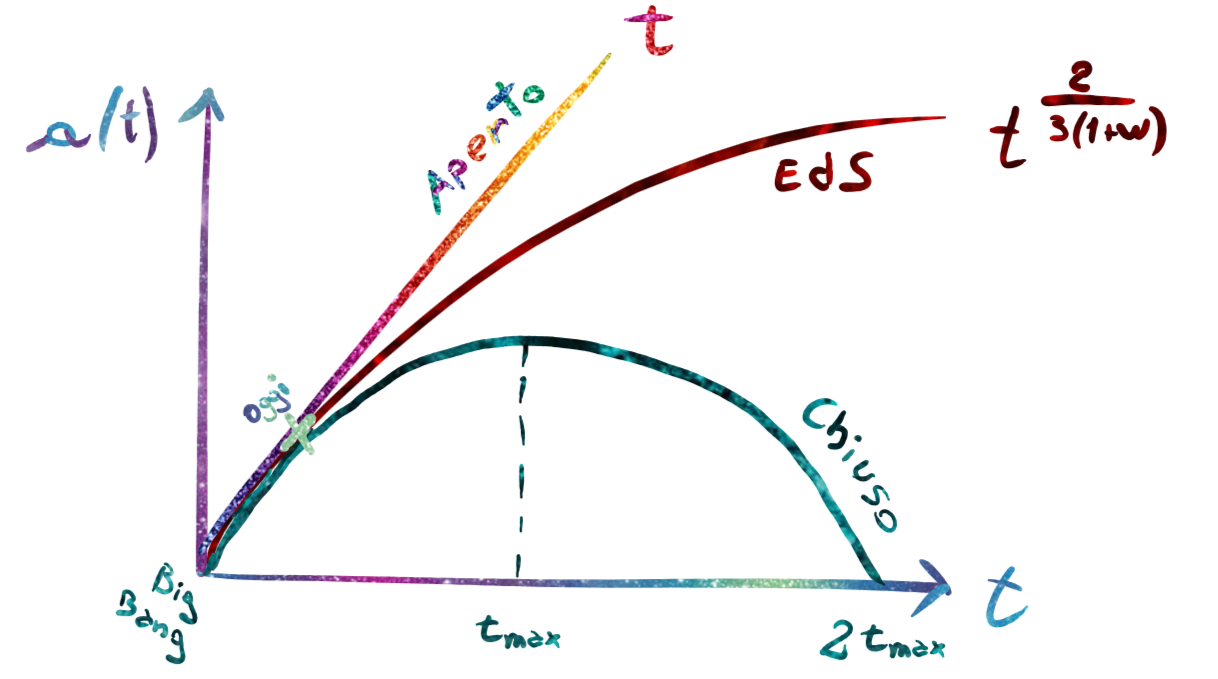
\includegraphics[width=.8\textwidth]{Pictures/2/modellia-t.png}
    \caption{Andamento di $a$ al variare del tempo per le tre geometrie nel caso di universo di Friedmann. Tutte e tre sono vincolate ad avere un Big Bang per le assunzioni del modello.}
    \label{fig:2at}
\end{figure}

Le soluzioni analitiche  si ricavano soltanto per il modello di Einstein De Sitter, ma nel caso di universi curvi si possono trovare delle soluzioni in forma parametrica, ossia sfruttando la relazione: 
$$
\left\{\begin{matrix}
y= f(y')\\ 
y'=p
\end{matrix}\right. \qquad \Leftrightarrow \qquad 
\left\{\begin{matrix}
x= \int \mathrm{d}p \frac{1}{p}\frac{\mathrm{d} f}{\mathrm{d} p}\\ 
y=f(p)
\end{matrix}\right.
$$
Non si troverà quindi la relazione formale di $y$ rispetto a $x$, ma saranno entrambi scritti in funzione di un terzo parametro $p$. Nel nostro linguaggio $x$ sarà il tempo e $y$ il fattore di scala, quindi la relazione tra $a$ e $t$ si studierà attraverso un terzo parametro.

Si assume $c=1$ e $w=0$, ossia universi di materia (di polvere) e si sostituisce la relazione (\ref{eq:rhoaw}) nella seconda equazione di Friedmann (\ref{eq:friedmann2}). Definendo il parametro $p:=\dot{a}$ e la costante $A:= 8\pi G ~\rho_0 ~ a_0^3 /3$, si ottiene:
\begin{equation*}\left\{
\def\arraystretch{1.5}
    \begin{array}{ll}
    t=-\int \mathrm{d}p \frac{2A}{(p^2+k)^2} \\
    a=\frac{A}{p^2+k}
\end{array}\right.
\end{equation*}

Si studia il caso in cui $k=+1$ ponendo $p:= \tan \theta \rightarrow \mathrm{d}p=\mathrm{d}\theta / \cos^2 \theta$ e $2\theta = \pi-\alpha$:
\begin{equation*}\left\{
\def\arraystretch{1.5}
    \begin{array}{ll}
    t=\frac{A}{2}(\alpha - \sin \alpha) \\
    a=\frac{A}{2}(1 - \cos \alpha)
\end{array}\right.
\end{equation*}

Applicando le definizioni di $\rho_{cr}$, $\Omega_0$ e la relazione $a_0^2 ~H_0^2 = (\Omega_0 -1)^{-1}$ (dalla \ref{eq:friedmannh0rho0}) si ottengono le soluzioni, che sono tutte le possibili combinazioni della coppia ($a,t$) al variare del parametro $\alpha$:
\begin{equation}\left\{
\def\arraystretch{1.5}
    \begin{array}{ll}
    a=\frac{a_0}{2} \frac{\Omega_0}{\Omega_0 -1}    (1 - \cos \alpha) \\
    t=\frac{1}{2H_0} \frac{\Omega_0}{(\Omega_0 -1)^{3/2}}  (\alpha - \sin \alpha)
\end{array}\right.
\end{equation}

Si ha $\dot{a}>0$ per $0<\alpha < \pi$, dopodiché la curva si richiude simmetricamente. L'età dell'universo prevista per questo modello è:
\begin{equation*}
    t_0 = \frac{1}{2H_0}\frac{\Omega_0}{(\Omega_0 -1)^{3/2}}\left ( \arccos{\left ( \frac{2-\Omega_0}{\Omega_0} \right )}  -\frac{2}{\Omega_0}\sqrt{\Omega_0-1} \right )
\end{equation*}
Si può verificare che l'età dell'universo (a parità di $H_0$) è sempre minore rispetto a quella dell'universo EdS :
\begin{equation}
t_0 = \mathfrak{C} \frac{1}{H_0}\qquad \mathfrak{C}< 2/3
\end{equation}

In modo simile è possibile trovare le soluzioni parametriche per gli universi di materia nel caso in cui $k=-1$ ($\Omega_0<1$): 
\begin{equation}\left\{
\def\arraystretch{1.5}
    \begin{array}{ll}
    a=\frac{a_0}{2} \frac{\Omega_0}{1-\Omega_0}    (\cosh \alpha -1) \\
    t=\frac{1}{2H_0} \frac{\Omega_0}{(\Omega_0 -1)^{3/2}}  (\sinh \alpha -\alpha)
\end{array}\right.
\end{equation}
\begin{equation}
t_0 = \mathfrak{C} \frac{1}{H_0}\qquad \mathfrak{C}> 2/3
\end{equation}
Come già osservato in precedenza, si ha un'espansione infinita con un comportamento asintotico $a\propto t $.

Tutte le soluzioni ricavate in questo paragrafo, che siano analitiche o parametriche, valgono soltanto nel caso in cui si considera un universo a un'unica componente. Per studiare l'effetto di più componenti le equazioni rimangono sotto forma di integrali e vanno risolte numericamente.

Sommario («Ok quello che stiamo facendo?»):
\begin{itemize}
    \item Soluzioni dei modelli di Friedmann per una sola componente;
    \item Soluzioni analitiche per EdS;
    \item Soluzioni parametriche per universi curvi di sola materia.
\end{itemize}

\subsection{Modelli a due componenti}
Dall'equazione (\ref{eq:hevolmulti}) si esplicita la quantità $\dot{a}=a_0 ~H_0 ~E /(1+z) = a ~H_0 ~E$ e la si inserisce nella relazione (quirefffs):
\begin{equation}
    \mathfrak{f}(r) = \int_{a}^{a_0} \frac{c ~\mathrm{d}a'}{a' ~\dot{a}'} = \frac{c}{H_0} \int_{a}^{a_0} \frac{\mathrm{d}a'}{E ~a'^2}
\end{equation}
dove $E(z) = \Omega_{0m}(1+z)^3 + \Omega_{\Lambda 0}$ per $\Omega_{tot}=1$. Nel caso di universo piatto, essendo $\mathfrak{f}(r)=r$ si ha:
\begin{equation}
    d_A = \frac{c}{H_0 (1+z)} \int^z_0 \frac{\mathrm{d}z}{E(z)}
\end{equation}
altrimenti è necessario applicare un arcoseno o un arcoseno iperbolico. A questo punto "si fa partire il cronometro", ossia si studia il legame tra tempo e redshift. Dalla (\ref{eq:hevol}) per la sola materia, $w=0$, si ha:
\begin{equation}
\dot{a}=a_0~H_0~\sqrt{\Omega_0 ~z +1} \label{eq:adotsolamateria}
\end{equation}
Tramite la relazione $1+z=a_0/a$ si ottiene il legame differenziale tra $t$ e $z$ e integrando:
\begin{align}
    t(z) &=\int_z^\infty \frac{1}{H_0}(1+z')^{-2}(\Omega_0 z'+1)^{-1/2}\mathrm{d}z' \\
    & \approx  \frac{1}{H_0 \sqrt{\Omega_0}}~\frac{2}{3} z^{-3/2} \qquad per\quad \Omega_0 z \gg 1
\end{align}
Siamo felici perché vicino al Big Bang (curvatura ininfluente) ritroviamo la dipendenza prevista dal modello EdS. Per più di un componente bisogna integrare la formula generale:
\begin{equation}
    \mathrm{d}t = - \frac{1}{H_0 ~E}\frac{1}{(1+z)}\mathrm{d}z
\end{equation}
La quantità "complementare" all'età dell'universo oggi è il \textbf{Lookback Time}:
$$
t_{LB}(z) = t_0 - t(z)
$$

Sia la densità, sia la densità critica possono dipendere dal tempo, a maggior ragione anche $\Omega$ non sarà costante nel tempo. Dalle equazioni (\ref{eq:hevol}) e (\ref{eq:hevol}) si può calcolare:
\begin{equation*}
    \Omega(z) = \frac{\rho(t)}{\rho_{cr}(t)} \qquad\rightarrow \qquad \Omega^{-1}(z) -1 = \frac{\Omega_0^{-1}-1}{(1+z)^{1+3w}}
\end{equation*}
che misura quanto dista dall'unità $\Omega (z)$ rispetto a quanto dista dall'unità oggi.


Se oggi $\Omega_0$ vale 1 (universo piatto), $\Omega(t)$ sarà sempre stato e sempre sarà 1. Se $\Omega_0 > 1$, allora $\Omega(z) > 1\quad \forall z$ e se $\Omega_0 < 1$, allora $\Omega(z) < 1\quad \forall z$. L'universo non può cambiare la sua geometria durante la sua evoluzione.
\begin{figure}[ht]
    \centering
    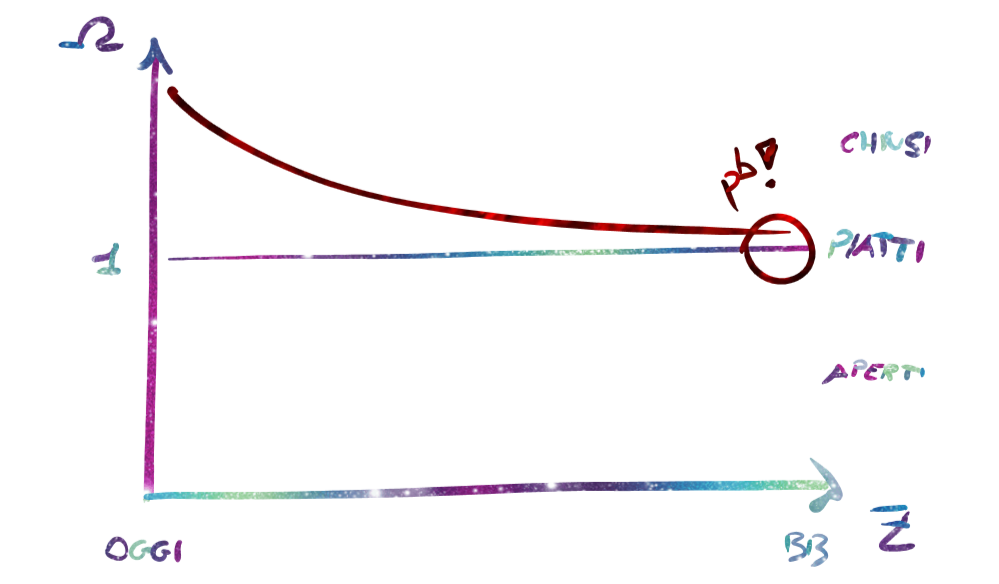
\includegraphics[width=.8\textwidth]{Pictures/2/omega-z.png}
    \caption{Andamento di $\Omega$ al variare del redshift per le tre geometrie nel caso di universo di Friedmann. Tutte e tre verso il Big Bang tendono a $\Omega = 1$.}
    \label{fig:2omegaz}
\end{figure}

Se si ha più di una componente, la formula generale da utilizzare è:
\begin{equation}
    \Omega (z) = \Omega_0 \frac{(1+z)^{3(1+w)}}{E(z)^2}
\end{equation}


\begin{definition}[Problema della Piattezza]
 Oggi si misura $\Omega_0 =1$ e già negli anni '70 si sapeva che $\Omega_0 \approx 1$. Ma dal Big Bang è passato talmente tanto tempo che, per avere oggi questo valore, doveva inizialmente valere $1$ con una precisione di $10^{-60}$ (valore estremamente innaturale). 
\end{definition}


\section{Orizzonte Cosmologico}
Ci si aspetterebbe che l'universo in connessione causale con noi osservatori sia $c\, \Delta t$, ma l'universo si espande! Si definisce quindi il \textit{raggio dell'orizzonte cosmologico (o delle particelle)} la quantità:

\begin{equation}
    R_H (t) = a(t) \int_0^t \frac{c\, \mathrm{d}t'}{a(t')}
\end{equation}
Per $a \rightarrow 0$ quando $ t \rightarrow 0$ pare accadere che $R_H \rightarrow \infty$ e questo implicherebbe che tutto l'universo al Big Bang fosse in connessione causale (che senso avrebbe definire un raggio?), ma questo non succede. Si può verificare mediante un opportuno cambio di variabile e l'utilizzo dell'equazione (\ref{eq:adotsolamateria}):
\begin{equation*}
    R_H (a) = a(t) \int_0^{a(t)} \frac{c\, \mathrm{d}a'}{a' \: \dot{a}'} \quad = \frac{2}{1+3w} \frac{c}{H_0\, \Omega_0^{1/2}} \left ( \frac{a}{a_0} \right)^{\frac{3(1+w)}{2}}
\end{equation*}
Quindi il raggio dell'orizzonte per $a \rightarrow 0$ non diverge. Si utilizza una sola componente, infatti come discuteremo a breve vicino al Big Bang domina soltanto la componente radiativa. Inoltre si ha:
\begin{equation}
    R_H (t) = \frac{2}{1+3w}\frac{c}{H_0}\frac{t}{t_0} = 3ct \left ( \frac{1+w}{ 1+3w} \right )= \left\{\begin{matrix}
3ct & w=0\\ 
2ct & w=\frac{1}{3}\: (BB)
\end{matrix}\right.
\end{equation}
Quindi cresce più velocemente di $ct$, ossia mette in comunicazione regioni più vaste di quanto ci aspettavamo. $R_H$ rappresenta la scala su cui bisogna considerare le interazioni causali (microfisica), al suo esterno agisce solo la gravità.

Un altro modo per definire l'orizzonte è la \textbf{Sfera di Hubble} ( o raggio dell'orizzonte effettivo), definita come la distanza che percorre la luce in un'unità di tempo tipica del tempo di espansione dell'universo ($1/H$): 
\begin{equation}
    \tilde{R}_H (t) = c\: \tau_{exp} = \frac{c}{H}
\end{equation}
Mentre la definizione precedente era una quantità integrale sulla sfera di espansione temporale, in questo caso si ha un valore istantaneo definito da $H(t)$. Per l'universo primordiale vale $R_H \equiv \tilde{R}_H (t)$. Nel caso di universi EdS si ha:
\begin{equation*}
    \tilde{R}_H (t) =  \frac{1+3w}{2} R_H
\end{equation*}
Il tempo tipico di espansione è fondamentale per decidere quali processi, in determinati periodi della storia dell'universo, possono essere considerati trascurabili o meno.

Si definisce invece \textit{raggio dell'orizzonte degli eventi} la quantità:
\begin{equation}
     R_H (t) = a(t) \int_t^\infty \frac{c\, \mathrm{d}t'}{a(t')}
\end{equation}
e stabilisce il raggio delle regioni dell'universo che al tempo $t$ entrano in connessione causale con l'osservatore. Questa quantità non è solitamente utilizzata in cosmologia. Tutti i modelli di Friedmann prevedono un Big Bang e un orizzonte cosmologico finito.

\section{Componenti Osservate nell'Universo}

\subsubsection{Galassie}
La funzione di luminosità di Schechter provvede una descrizione parametrica della densità spaziale delle galassie in funzione della loro luminosità.
$$
\phi (L) = \frac{\phi_*}{L_*} \left ( \frac{L}{L_*}  \right)^{-\alpha}e^{-L/L_*}
$$
\chapterimage{head2.png} % Chapter heading image
\chapter{Evoluzione termica dell'Universo}\label{3:ch}


\section{Temperatura e redshift}
La materia e la radiazione hanno avuto la stessa temperatura finché le interazioni sono state sufficientemente elevate per mantenere una condizione di equilibrio. Per verificare se questo accade si utilizza come tempo scala il tempo collisionale: $\tau_{coll}=(c\sigma n)^{-1}$. Oggi buona parte della materia è in forma neutra per cui possiamo assumere $\sigma \rightarrow \sigma_H$, inoltre  esprimere: $n_0 = \rho_0 / m_P$. Questa quantità va confrontata col tempo tipico di espansione dell'universo $\tau_{exp} \sim 1/H_0$. Si trova che, oggi, $\tau_{coll} \gg \tau_{exp}$, per cui $T_{m0} \neq T_{r0}$ e possiamo considerarle come componente separate.
L'andamento della temperatura in funzione del redshift si ricava tramite l'equazione di adiabaticità:
$$
\mathrm{d}(\rho c^2 a^3) = - p_m\: \mathrm{d}a^3
$$




\subsection{Temperatura della materia}
Si hanno due contributi alla densità di energia: l'energia di massa e l'energia termica. Per esprimere la pressione si fa uso dell'assunzione di gas perfetto. 
$$
 \rho c^2 = \rho_m c^2 + \frac{3}{2}k_B T_m \frac{\rho_m}{m_P} \qquad p_m = \frac{\rho_m k_B T_m}{m_P}
$$
Sostituendo questi valori nell'equazione di adiabaticità si ottiene:
\begin{equation}
    T_m = T_{0m} (1+z)^2 = T_{0m}\left ( \frac{a_0}{a}\right )^2  \propto a^{-2}
\end{equation}
Questo andamento era atteso poiché la condizione di adiabaticità implica $TV^{\gamma -1} = cost$, che per $\gamma=5/3$ restituisce lo stesso andamento appena ottenuto.

\subsection{Temperatura della radiazione}
In questo caso la densità di energia è ottenibile dalla funzione di corpo nero:

$$
 \rho_R c^2 = \sigma T_R^4 \qquad p_R = \frac{1}{3}\rho_R c^2 = \frac{\sigma T_R^4}{3}
$$
Sostituendo questi valori nell'equazione di adiabaticità si ottiene:
\begin{equation}
    T_R = T_{0R} (1+z) = T_{0R}\left ( \frac{a_0}{a}\right )  \propto a^{-1}
\end{equation}

Quindi materia e radiazione, quando separate, viaggiano su adiabatiche diverse.




Il tempo scala delle collisioni evolve come $\tau_{coll}=(c\sigma n)^{-1} \propto \rho_b^{-1}$. Dato che la densità dei barioni $\rho_b \propto z^3$ si ha che $\tau_{coll}\propto (1+z)^{-3}$. I tempi-scala in gioco sono quindi:
\begin{align*}
    & \tau_{coll} \propto (1+z)^{-3} \\
    & \tau_{exp, \, m} \propto (1+z)^{-3/2} \\
    & \tau_{exp, \, R} \propto (1+z)^{-2}
\end{align*}

Avvicinandosi al Big Bang, $\tau_{coll}\ll \tau_{exp}$, quindi la condizione di equilibrio è verificata. Inoltre andando a temperature più alte cambia la sezione d'urto $\sigma_H \rightarrow \sigma_T$ e la sezione d'urto Thomson è estremamente efficiente a fare collisioni e la materia diventa relativistica. Materia e radiazione erano quindi termicamente accoppiate. Esiste un valore di $z$ per cui si disaccoppiano, \textit{decoupling}, e vale circa $z_{dec}\approx 1000$. Con la temperatura che diminuisce si ha anche la ricombinazione (neutralizzazione) dell'idrogeno e si forma la superficie di ultimo scatter.

\section{Temperatura pre-disaccoppiamento}
Ci si aspetterebbe che, essendo materia e radiazione accoppiate, la temperatura evolva con un andamento intermedio tra le due, cioè $T\propto a^x$ con $x\in (-2, -1)$. L'accoppiamento è atteso osservando gli andamenti di $T_m$ e $T_R$ e assumendo che per $t<t_{decoup}$ la condizione $T_m = T_R$ venga mantenuta. 

Dalla condizione di adiabaticità, considerando tutti i contributi di materia e radiazione si ha:
\begin{equation}
    \mathrm{d} \left [ a^3    \left( \rho_m c^2 + \frac{3}{2}k_B T \frac{\rho_m}{m_P} + \sigma T^4 \right)  \right] = - \mathrm{d} \left [ a^3    \left( \frac{\rho_m k_B T_m}{m_P} + \frac{\sigma T_R^4}{3}  \right)  \right]
\end{equation}

Introducendo la quantità:
\begin{equation}
    \sigma_{RAD}= \frac{4}{3} \frac{m_P ~\sigma ~T^3}{k_B ~\rho_m}
\end{equation}

e ricordando che $\mathrm{d} (\rho_m a^3) = 0$, si può ottenere la relazione:
\begin{equation}
\frac{ \mathrm{d}T}{T}= - \frac{ \mathrm{d}a}{a} \: \frac{1+\sigma_{RAD}}{\frac{1}{2} +\sigma_{RAD}}
\end{equation}

Dal momento che la quantità $\sigma_{RAD}$ dipende dal tempo e dalla temperatura, non è sempre possibile risolvere analiticamente questa equazione. Si può però verificare che, dopo il disaccoppiamento ($T=T_{RAD}$), il valore $\sigma_{RAD}=cost=\sigma_{RAD, \, 0}$. Il valore esatto è:
\begin{equation*}
    \sigma_{RAD, \, 0} \simeq 1.35 \cdot 10^8 \; (\sigma_{ob}h^2)^{-1}
\end{equation*}

Il fatto che $\sigma_{RAD}$ sia costante ed estremamente alto, garantisce che l'andamento al momento del disaccoppiamento sia $\mathrm{d}T / T \propto \mathrm{d}a / a$ per cui per $t<t_{decoup}$ si ha: 
\begin{equation}
T \propto (1+z) \propto a^{-1} 
\end{equation}

A maggior ragione per $t$ piccoli, a causa dell'aumento di $T$, emerge sempre di più il comportamento relativistico della materia. Quindi, a differenza di quanto era atteso, è solo il comportamento della radiazione a dominare a queste epoche.

\begin{figure}[h]
    \centering
    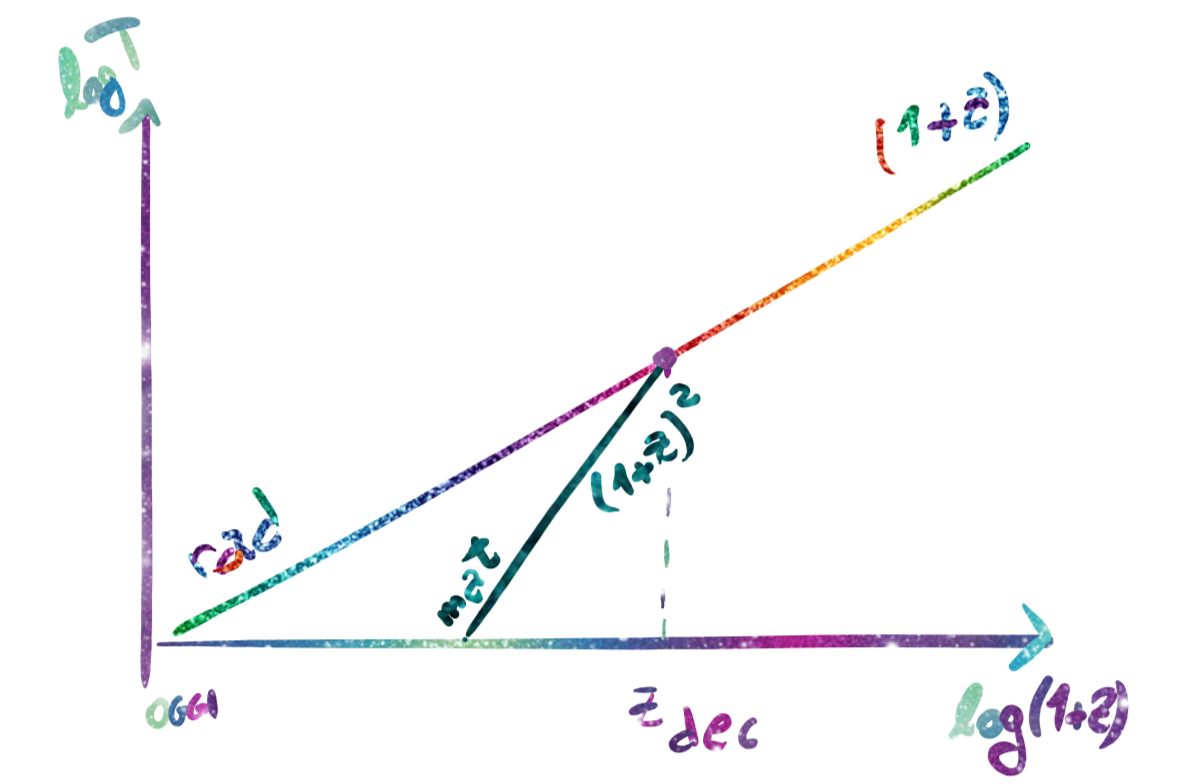
\includegraphics[width=.8\textwidth]{Pictures/3/logT-z.png}
    \caption{Andamento della Temperatura di materia e radiazione pre e post disaccoppiamento.}
    \label{fig:3logzt}
\end{figure}

La quantità $\sigma_{RAD}$ viene detta \textit{entropia della radiazione per barione}, corrisponde infatti al rapporto fra la densità di entropia della radiazione $S_R= (\rho c^2 + p_R)/T$ e il numero dei barioni esistenti (reso adimensionale dividendo per $k_B$). Quindi si ha che "c'è un sacco di entropia nella radiazione rispetto al numero di particelle barioniche nell'universo". Questo concetto può anche essere visto studiando la densità di capacità termica $\mathfrak{C}$:
$$
\rho_R ~\mathfrak{C}:=\frac{\partial \left (\rho_R ~c^2  \right )}{\partial T}=4\sigma T^3 \qquad\qquad \rho_m ~\mathfrak{C}:=\frac{\partial\left ( \frac{3}{2}\frac{\rho_m k_B T}{m_P}  \right )}{\partial T} = \frac{3}{2}\frac{\rho_m k_B}{m_p}
$$
Il rapporto tra queste due quantità corrisponde proprio a $2\sigma_{RAD}$. Questo ci sta dicendo che la capacità termica è dominata dalla componente radiativa.
Inoltre si introduce un parametro importante, $\eta$:
\begin{equation}
    \eta = \frac{\# ~nucleoni}{\# ~fotoni} = \frac{\rho_b}{m_p} \frac{1}{ \left( \frac{k_B T}{\hslash c}\right)^3 \int \frac{8 \pi \lambda^2}{e^x - 1} \mathrm{d}x} \propto \frac{\rho_m}{m_P T^3}
\end{equation}

In particolare si ha:
\begin{equation}
    \sigma_{RAD, \, 0 } = 3.6 ~ \eta_0^{-1}
\end{equation}

Il valore grande di $\sigma_{RAD}$ è dovuto al fatto che oggi il numero di fotoni è circa $10^8$ volte il numero di nucleoni (motivo per cui la capacità termica della radiazione è maggiore). Questo è strettamente legato ad un fenomeno accaduto nell'universo primordiale: l'\textbf{anisotropia barioni-antibarioni}. Sotto l'ipotesi di conservazione del numero barionico vale la relazione $(n_b - n_{\overbar{b}} )~a^3 = n_{b, \,0}~a_0^3$ poiché oggi non osserviamo antibarioni. Inoltre nell'univeso primordiale $n_b \simeq n_{\overbar{b}} \simeq n_\gamma $, dove $n_\gamma $ è il numero dei fotoni; una quantità adimensionale per misurare l'anisotropia è:
\begin{equation}
    \frac{n_b - n_{\overbar{b}}}{n_b + n_{\overbar{b}}}= \frac{n_b - n_{\overbar{b}}}{2 n_\gamma} \equiv \frac{n_{b, \,0}}{2n_{\gamma, \,0}} \propto \sigma_{RAD, \, 0 }^{-1}
\end{equation}
Questo implica che nell'universo primordiale il numero di barioni e antibarioni non era esattamente uguale: a causa della piccola differenza sono sopravvissuti i pochi barioni in un mare di fotoni prodotti per annichilazione. Per esempio: $10^8$ fotoni + $10^8$ antibarioni + $10^8 +1 $ barioni avrebbero generato $3\cdot 10^8$ fotoni e $1$ barione, valore simile al rapporto osservato. Quali sono i meccanismi in grado di produrre una sì piccola differenza tra $b$ e $\overbar{b}$?

\vspace{1em}
La temperatura verrà utilizzata come cronometro per studiare la storia evolutiva dell'universo, infatti è in base ad essa che si sceglie quale fisica utilizzare. Per qualsiasi particella di massa $m$ esiste sempre una $T_{eq}$ alla quale l'energia termica $k_BT_{eq}$ è uguale all'energia di massa $2m c^2$. Una coppia elettrone-positrone può esistere soltanto se $T\gtrsim T_{eq}$ altrimenti dominerebbe il processo di annichilazione (produzione di 2 fotoni). Dalla relazione si può concludere che \textbf{a temperature elevate (universo primordiale) possono soltanto esistere particelle di grande massa}. Dal Big Bang ad oggi sarà possibile, semplificando, distinguere l'era adronica e poi l'era leptonica.
\vspace{2em}

I due momenti fondamentali fino ad ora discussi sono:
\begin{example}[Equivalenza Materia-Radiazione]
    $\rho_m (z_{eq})=\rho_R(z_{eq})$
\end{example}
Precedentemente si è ricavato: $1+z_{eq}=\Omega_{0m}/\Omega_{0R}$, dove per $\Omega_{0R}$ si include anche la componente relativistica della materia (e.g. neutrini). Dalla relazione tempo-redshift:
$$
t_{eq} \approx 10^4 ~\mathrm{yr}
$$
L'epoca dominata dalla radiazione è un'inezia! Le equazioni di Friedmann per la sola materia non portano a grossi errori di calcolo.

\begin{example}[Disaccoppiamento]
    Tempo dopo il quale $T_m(t)\neq T_R(t)$
\end{example}
Quando la temperatura scende sotto una certa soglia si forma idrogeno neutro e $\sigma_T \rightarrow \sigma_H$. Questo avviene a:
$$
t_{dec} \approx 3\cdot 10^5 ~\mathrm{yr} \qquad\qquad z \approx 10^3
$$
Il realtà si vedrà che il tempo a cui avviene la ricombinazione è diverso dal tempo a cui avviene il disaccoppiamento e dipende dalle specie chimiche considerate.


\chapterimage{/4/head.jpg} % Chapter heading image
\chapter{Cinque Problemi del Modello Standard}\label{4:ch}

Ci sono alcuni problemi radicati nel modello del Big Bang che vengono in parte risolti con il paradigma dell'inflazione.

\section{Problema dell'origine (Big Bang)}
Il fenomeno del Big Bang è implicito nelle equazioni di Friedmann (relatività generale + spazio omogeneo e isotropo (RW) + fluido perfetto). Ossia assumendo l'andamento $a\propto t^\beta$, $\ddt{a}<0$ e $\dt{a}_0 >0$ come osservato, la funzione monotona crescente $a(t)$ prima o poi deve sbattere sull'asse x.   
Il Big Bang è però matematicamente molto brutto perché per $t\rightarrow 0$ si ha $\rho \rightarrow \infty$, $H \rightarrow \infty$ e $T \rightarrow \infty$, questo può essere evitato in 3 modi:
\vspace{0.5em}
\begin{enumerate}
    \item Ponendo $\ddt{a}>0$ (flesso) $\Leftrightarrow w<-1/3$. Nella fisica ordinaria questo non è possibile ed è quindi necessario introdurre la costante cosmologica. Tuttavia, le misurazioni della costante cosmologica vincolano il flesso a tempi tardi ($z=0.6$), lontano dal Big Bang. È quindi necessario introdurre un'ulteriore componente sconosciuta che generi un flesso vicino al Big Bang ($@ \_ @$).
    \item Abbandonando l'ipotesi di fluido perfetto includendo effetti di viscosità (bulk $\xi$ e shear $\eta$) e di conduzione. Le equazioni di Eulero viscose sono: $$ \rho \left ( \frac{\partial v}{\partial t} + (v \cdot\nabla)v \right )= -\nabla p +\eta \nabla^2v + \left ( \xi + \frac{\eta}{3} \right )\nabla(\nabla\cdot v). $$ Si può dimostrare che l'introduzione della shear viscosity o della conduzione porterebbero alla violazione di omogeneità e isotropia.
    \item Abbandonando l'ipotesi di omogeneità e isotropia (modelli di Bianchi).
\end{enumerate}

Si preferisce da un punto di vista pratico rimanere nella condizione di avere omogeneità e isotropia, pur dovendo affrontare il problema di giustificare la singolarità.

\subsection{Scala di Planck}
Sfruttando dimensionalmente il principio di indeterminazione di Heisemberg:
$$
\Delta E \Delta t \leq \hslash \quad \rightarrow \quad (G t_P^2)^{-1} (c t_P)^{3}c^2 t_P \approx \hslash \quad \rightarrow \quad t_P \approx \sqrt{\frac{\hslash G}{c^5}} \approx 10^{-43}~\mathrm{s}
$$
Per $t<t_P$ è necessario quantizzare la gravità, problema ancora aperto. La trattazione che segue sarà quindi svolta a partire dal tempo di Plank. Alcune quantità fondamentali legate questo istante sono:
\begin{equation}\left\{
    \def\arraystretch{1.5}
        \begin{array}{ll}
        T_P \simeq 10^{32}~\mathrm{K} \\
        E_P \simeq 10^{19}~\mathrm{GeV} \\
        n_P \simeq 10^{98}~\mathrm{cm}^{-3} \\
        m_P \simeq 10^{-5}~\mathrm{g} \\
        \rho_P \simeq 10^{93}~\mathrm{g\: cm}^{-3}  \\
        l_P \simeq 10^{-33}~\mathrm{cm} \\
        \sigma = (entropia) = 1 
    \end{array}\right. \label{eq:unitaplanckiane}
\end{equation}
Il valore unitario dell'entropia simula la presenza di una sola particella (1 g.d.l.), sarà quindi necessario a un certo momento trovare un meccanismo fisico in grado di creare particelle.  

\subsubsection{Tempo di Compton}
È il l'intervallo di tempo (o lunghezza) sopra al quale possiamo ignorare gli effetti quantistici:
\begin{equation}
    t_C = \frac{\hslash}{mc^2} \quad \rightarrow \quad l_C =  \frac{\hslash}{mc}
\end{equation}

\subsubsection{Tempo di Schwarzschild}
È la scala alla quale la velocità di fuga è pari alla velocità della luce:
\begin{equation}
    l_S =  \frac{2Gm}{c^2}  \quad \rightarrow \quad   t_S = \frac{2Gm}{c^3} 
\end{equation}


\subsubsection{Tempo di Planck}
È il momento in cui la scala di Schwarzschild corrisponde alla scala Compton $t_C(m_P)=t_S(m_P)$ e da questa uguaglianza si definisce la massa di Planck. In altre parole: il tempo che descrive la gravità è esattamente uguale al tempo che descrive gli effetti quantistici, per le fasi successive si può ignorare la meccanica quantistica.

L'energia emessa da un buco nero dipende dalla sua temperatura (legata alla \textbf{radiazione di Hawking}) , $T=10^{-7} (M/\msun)^{-1}$ K. Il tempo tipico di evaporazione di un buco nero vale: $\tau_{evap}=10^{10} (M/10^{15}~\textrm{g})^{3} $ yr. Si può calcolare che il tempo di evaporarione di un buco nero di massa pari alla massa di Planck vale esattamente $t_P$. Questo apre la possibilità di pensare che prima del tempo di Planck vi fosse un continuo emergere ed evaporare di buchi neri nessuno dei quali poteva sopravvivere. A causa di una fluttuazione quantistica, uno di questi buchi neri è sopravvissuto per un tempo maggiore di $t_P$ ed è diventato il nostro universo. Questa è una delle possibilità adottate nei modelli per evitare il problema della singolarità. 





\section{Problema dell'orizzonte}
Assumendo $a\propto t^\beta$ si può osservare che il raggio dell'orizzonte (\ref{eq:raggioriz}) non diverge solo per $\beta < 1$. La divergenza implica che tutto l'universo sia in connessione causale. Inoltre, confrontando $\ddt{a}\propto a~\beta (\beta-1) ~t^{-2} $ con la prima equazione di Friedmann, si ha che il Big Bang esiste, cioè: $\ddt{a} < 0 \Leftrightarrow 0 < \beta < 1$. La condizione per avere un Big Bang è necessariamente implicata dall'avere un orizzonte cosmologico. 

Il problema dell'orizzonte deriva dall'osservazione della quasi perfetta isotropia della CMB. Affinché la CMB si possa ``uniformare'' su una data scala, è necessario che questa sia all'interno dell'orizzonte (ossia in connessione causale). Confrontando la scala dell'orizzonte con quella della CMB al momento dell'ultimo scattering fra fotoni ed elettroni ($z_{LS}\approx 10^3$):

\begin{equation*}
R_H = \frac{3(1+w)}{1+3w} ~c ~t_{LS} \approx  3 ~c ~t_0 ~ (1+z_{LS})^{-3/2} \qquad\qquad r_{LS} = \frac{c ~(t_0 - t_{LS})}{1+z_{LS}} \approx \frac{c ~t_0}{z_{LS}}
\end{equation*}

si ha la relazione: $R_H(z_{LS}) = 3 ~r_{LS} ~z_{LS}^{-1/2} \approx 0.1 ~r_{LS} $. Questo è in conflitto con l'osservabile (CMB), che deve essere stato prodotto in condizioni di connessione causale. Si cerca una soluzione matematico-grafica utilizzando un altro raggio, quello della sfera di Hubble ($\tilde{R}_H (t) = c/H $) che ha un valore pressoché equivalente al precedente nell'universo primordiale ed è più facile da studiare. Per graficare le soluzioni si utilizzano le quantità riscalate a meno dell'espansione (comoventi), $R_{H,c} = c ~a_0 / \dt{a}$ (vale comunque $ \tilde{R}_{H,c} \approx R_{H,c}$). 

Calcolandone la derivata si può notare che $\dt{R}_{H, c}=- c ~a_0 ~\ddt{a} / \dt{a}^2 \propto - \ddt{a}$. Per cui, nei modelli di Friedmann ($\ddt{a}<0$), il raggio della sfera di Hubble comovente $\tilde{R}_{H,c} (t)$ è una funzione monotona crescente. Data una scala qualsiasi, si può determinare il $t'$ in seguito al quale tale scala è completamente in connessione causale (Fig. \ref{fig4:hubblesphere}). 

\begin{figure}[ht]
    \centering
    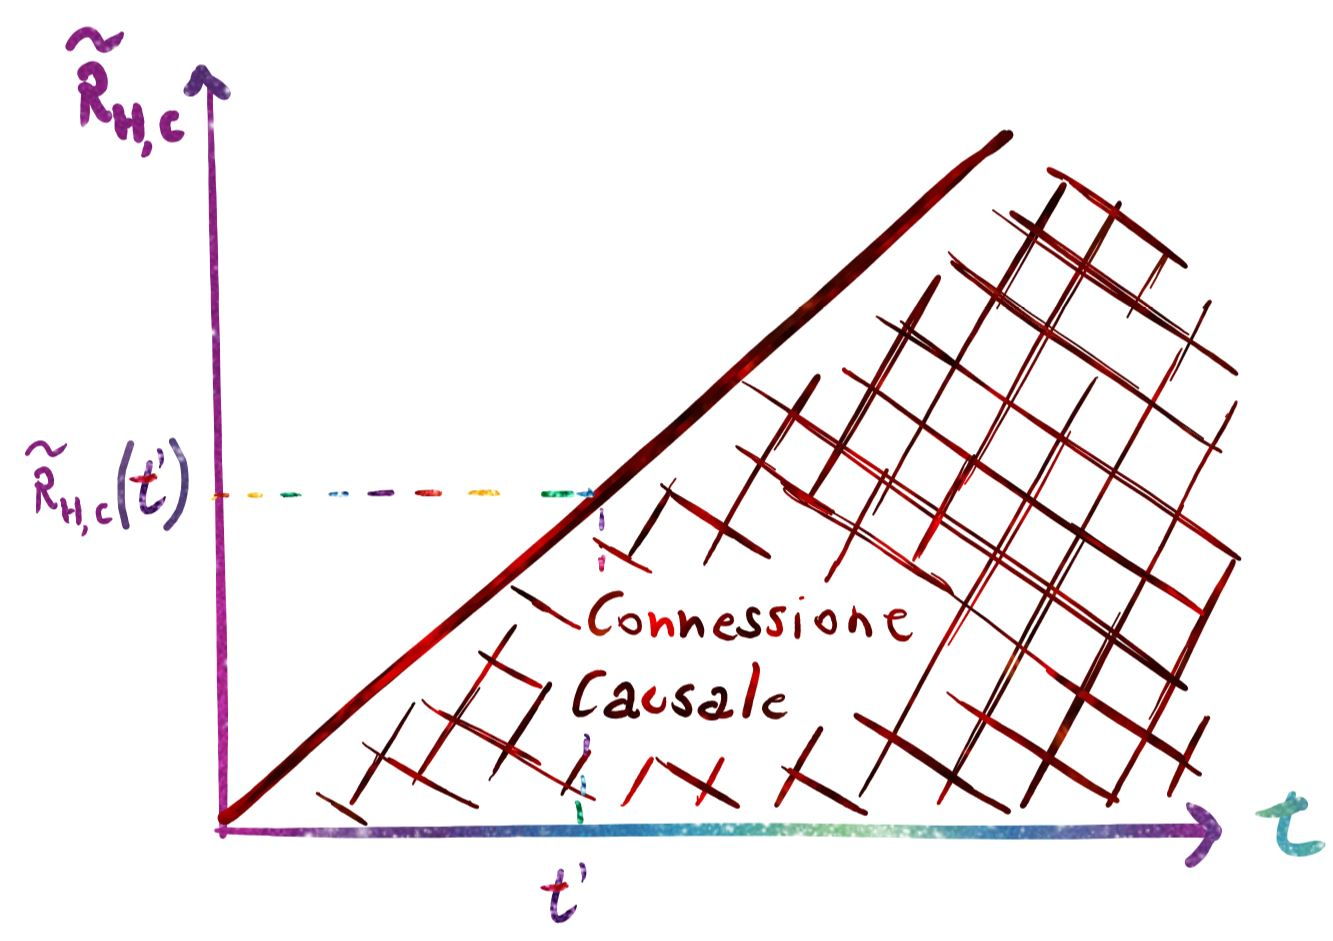
\includegraphics[width=.8\textwidth]{Pictures/4/rsferahubble-t.jpg}
    \caption{Andamento del raggio della sfera di Hubble comovente per universi con $\ddot{a}<0$.}
    \label{fig4:hubblesphere}
\end{figure}

Il problema può essere risolto assumendo che esista un periodo, $t_i<t<t_f$, in cui la curva diventa monotona decrescente (\textbf{periodo inflazionario}). In questo modo può esistere un intervallo entro il quale una data scala è stata in connessione causale (l'universo ha avuto modo di raggiungere l'equilibrio termico), anche se oggi la osservo fuori dall'orizzonte. Nel periodo inflazionario è necessario avere $\dt{R}_{H, c}<0 \rightarrow \ddt{a}>0  \rightarrow w <-1/3$ per un periodo sufficiententemente lungo (Fig. \ref{fig4:hubblespheremod}). (Passando a coordinate comoventi si è fattorizzata via l'espansione dell'universo, per questo il raggio dell'orizzonte comovente può decrescere!)

Dall'equazione (\ref{eq:hevol}), assumendo $\OmegaO = 1$ (universo primordiale) e definendo $s=3(1+w)/2$ si può ottenere, integrando per separazione delle variabili:
\begin{equation}
    a(t)=a_i \left( 1+s(t-t_i) ~H(t_i)\right)^{1/s}
\end{equation}
Al variare del parametro $w$ si ha:
\begin{equation}a(t) \propto\left\{
    \def\arraystretch{1.5}
        \begin{array}{lcll}
            t^{1/s} & -1 < w < -\frac{1}{3} &\mathbf{sub-inflazione} & \dt{H}<0 \\
            \exp (t/\tau)&  w=-1 & \mathbf{inflazione} & \dt{H}=0 \\
            (cost-t)^{1/s} & w<-1 & \mathbf{super-inflazione} & \dt{H}>0 \\
    \end{array}\right.
\end{equation}
\begin{figure}[ht]
    \centering
    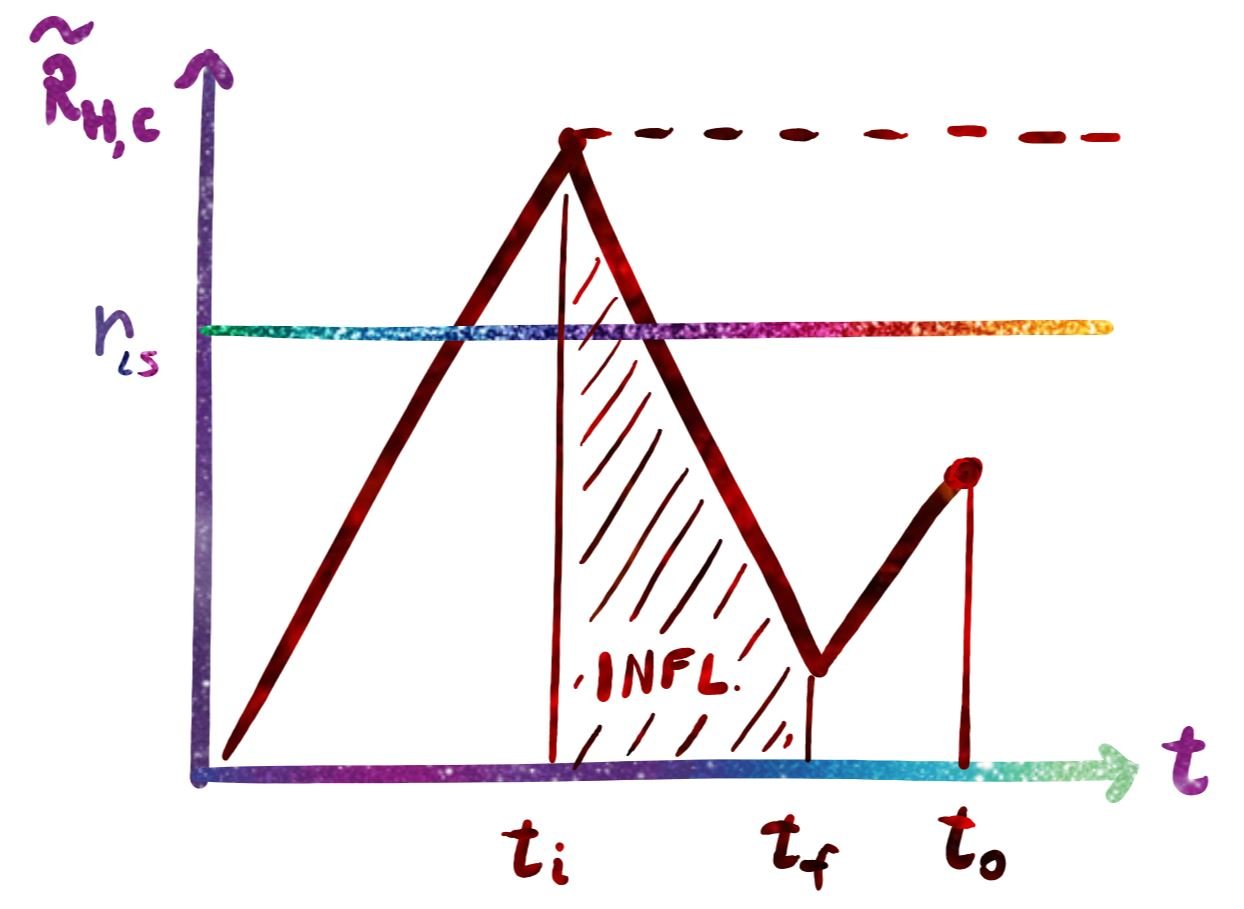
\includegraphics[width=.7\textwidth]{Pictures/4/pbhorsol.jpg}
    \caption{Soluzione al problema dell'orizzonte. $r_{LS}$ è il raggio della scala al momento dell'ultimo scattering. Oggi appare fuori dall'orizzonte, ma in passato ha avuto modo di sguazzarci, pertanto la CMB appare quasi uniforme.}
    \label{fig4:hubblespheremod}
\end{figure}

Nei primi due casi l'espansione è a legge di potenza, nel terzo caso è esponenziale. Gli andamenti di $\dt{H}(t)$ sono stati ricavati dalla relazione:
\begin{equation*}
    \ddt{a}= a\dt{H} + \frac{\dt{a}^2}{a} = a \left(  \dt{H} + H^2\right)
\end{equation*}

\subsubsection{Stima della durata dell'Inflazione}
La condizione è che la sfera di Hubble comovente all'inizio dell'inflazione $\tilde{R}_{H,c}(t_i)$ deve essere molto (per evitare problemi antropocentrici) più grande della sfera di Hubble oggi ${R}_{H,c}(t_0)$.
\begin{equation*}
\frac{c ~a_0}{H_i ~a_i} \gg \frac{c}{H_0} \quad \rightarrow \quad a_0 ~H_0 \gg a_i ~H_i
\end{equation*}

Attraverso l'equazione (\ref{eq:hevol}) si può esprimere come la relazione è variata nel tempo avendo cura di separare i periodi in base al proprio $w$:
\begin{equation*}
\frac{a_i ~H_i}{a_f ~H_f}\quad ^{[w<- \frac{1}{3}]} \qquad\ll\qquad \frac{a_0 ~H_0}{a_f ~H_f}\quad = \quad\frac{a_0 ~H_0}{a_{eq} ~H_{eq}} \quad ^{[w=0]}\quad \times \quad\frac{a_{eq} ~H_{eq}}{a_f ~H_f} \quad ^{[w= \frac{1}{3}]}\quad
\end{equation*}
per cui:
\begin{equation}
    \left( \frac{a_f}{a_i}\right)^{-(1+3w_{infl})} \quad\gg\quad \frac{a_0}{a_{eq}} \left( \frac{a_{eq}}{a_f}\right)^2 \simeq 10^{60} ~z_{eq}^{-1} \left( \frac{T_f}{T_P}\right)^2
\end{equation}
Questo valore stabilisce di quanto deve essere variato il fattore di scala durante l'inflazione per risolvere il problema dell'orizzonte. La stessa variazione viene parametrizzata attraverso il cosiddetto \textbf{numero di e-folding} $N_{ef}=\ln (a_f/a_i)$:

\begin{equation}
    N_{ef} \gg \frac{60}{\left | 1+3w_{infl}   \right |} \left(  2.3 + \frac{1}{30}\ln\frac{T_f}{T_P}-\frac{1}{60}\ln z_{eq}  \right) \quad \rightarrow \quad  N_{ef} \gg 60
\end{equation}
Questo corrisponde ad un aumento del volume dell'universo di $180$ dex.

\newpage
\noindent Morale, il problema dell'orizzonte è quindi risolto se:
\begin{itemize}
    \item Si assume che esiste un periodo in cui l'universo è in espansione accelerata;
    \item La durata di questo periodo è sufficiente per far sì che $N_{ef} \gg 60$;
    \item Si trova una giustificazione fisica per questa soluzione matematica.
\end{itemize}

\section{Problema dell'età dell'universo (o della piattezza)}
La prima equazione di Friedmann (\ref{eq:friedmann2}) è stata interpretata dal punto di vista newtoniano come l'equilibrio tra un termine cinetico e un termine potenziale determinato dalla costante $k$. Nell'epoca primordiale (era radiativa) tutte le forze sono unificate e non ci sono scale privilegiate: l'unico tempo scala è il tempo di Planck. Ci si aspetterebbe quindi che: per un universo chiuso $2t_{max}\sim t_P$; per un universo aperto $t^* \sim t_P$ dove $t^*$ è il tempo oltre al quale la curvatura è trascurabile e $a\propto t$ asintoticamente. In questo secondo caso si può utilizzare la temperatura della CMB $T_r\propto a^{-1}$ per misuare l'età dell'universo attesa: $t_0 = t_P T_P / T_0\simeq 10^{-43+32-0}\simeq 10^{-11}$ s. La durata dell'universo palesemente maggiore dei due risultati ottenuti potrebbe quindi essere dovuta all'insolito fatto che fra tutti i valori possibili, si abbia esattamente $\OmegaO=1$ (universo piatto). 

In particolare, affinché oggi valga $\OmegaO=1$, ai tempi di Planck ($w=1/3$) si doveva avere:
$$
    \OmegaTOT (t_P) = 1+\frac{ \left| \OmegaO -1 \right|}{\OmegaO(1+z_P)^2} = 1 + \left| \OmegaO -1 \right|\cdot 10^{-60}
$$
Avere un valore così stringente nei modelli non è bello e viene definito \textbf{problema di fine-tuning}. Supponendo che il valore differisse anche poco dall'unità, $\OmegaTOT (t_P) =1.01$, oggi si avrebbe $\OmegaO=10^{58}$ e già negli anni `70 ($\OmegaO\simeq 1 \pm 10$) i cosmologi non sarebbero stati contenti.

Attraverso l'equazione (\ref{eq:2omega0k}) si possono sviluppare le seguenti relazioni:
\begin{equation}
    H_0^2 \left ( 1-\OmegaO \right ) = -\frac{kc^2}{a_0^2} \equiv \frac{a^2}{a_0^2} \left( H^2 - \frac{8}{3}\pi G \rho\right) \quad \rightarrow \quad \frac{a^2}{a_0^2} H^2 (1-\Omega) = cost
\end{equation}
Dividendo la quantità costante per $T_0$ e moltiplicando per $(\hslash /k_B)^2$ per renderla adimensionale:
\begin{equation}
    |\varepsilon (t) | := |k| \left( \frac{\hslash c}{a k_B T}\right)^2 = \frac{H_0^2 |\OmegaO -1|}{T_{r\, 0}^2}\frac{\hslash^2}{k_B^2} \simeq | \OmegaO -1 | \cdot 10^{-58} < 10^{-57}
\end{equation}

A questo punto si può porre a zero senza problemi richiedendo $k=0$ per tutta la durata dell'universo. Questa quantità può essere legata all'entropia dell'universo (ossia della radiazione per l'universo primordiale):
\begin{equation}
    \sigma_u = \frac{S_R ~a^3}{k_B} \simeq \left( \frac{k_B Ta}{\hslash c} \right)^3 \simeq |\varepsilon (t) |^{-3/2} > 10^{86}
\end{equation}

Un valore così elevato dell'entropia rispetto a quello del tempo di Planck ($\sigma=1$), richiede la creazione di un numero elevatissimo di particelle (che giustificherà la piattezza). 
Il problema può essere risolto assumendo che esista un intervallo di tempo durante il quale il valore di $\Omega$ si avvicini all'unità, contrariamente all'evoluzione predetta dai modelli di Friedmann. Affinché questo avvenga (cfr. eq. \ref{eq:2omega0k}) bisogna avere $w<-1/3$ (espansione accelerata, e.g. inflazione!), di durata sufficiente. La condizione da imporre è $(1-\Omega_i^{-1})/(1-\OmegaO^{-1})\ge 1$, ossia $N_{ef}\ge 60$. Con la condizione del paragrafo precedente,  $N_{ef}\gg 60$, $\Omega$ si schiaccia ancora di più a 1 (nel remoto caso in cui si misurasse $\Omega=0.98$ si butterebbe via il modello).

\begin{figure}[ht]
    \centering
    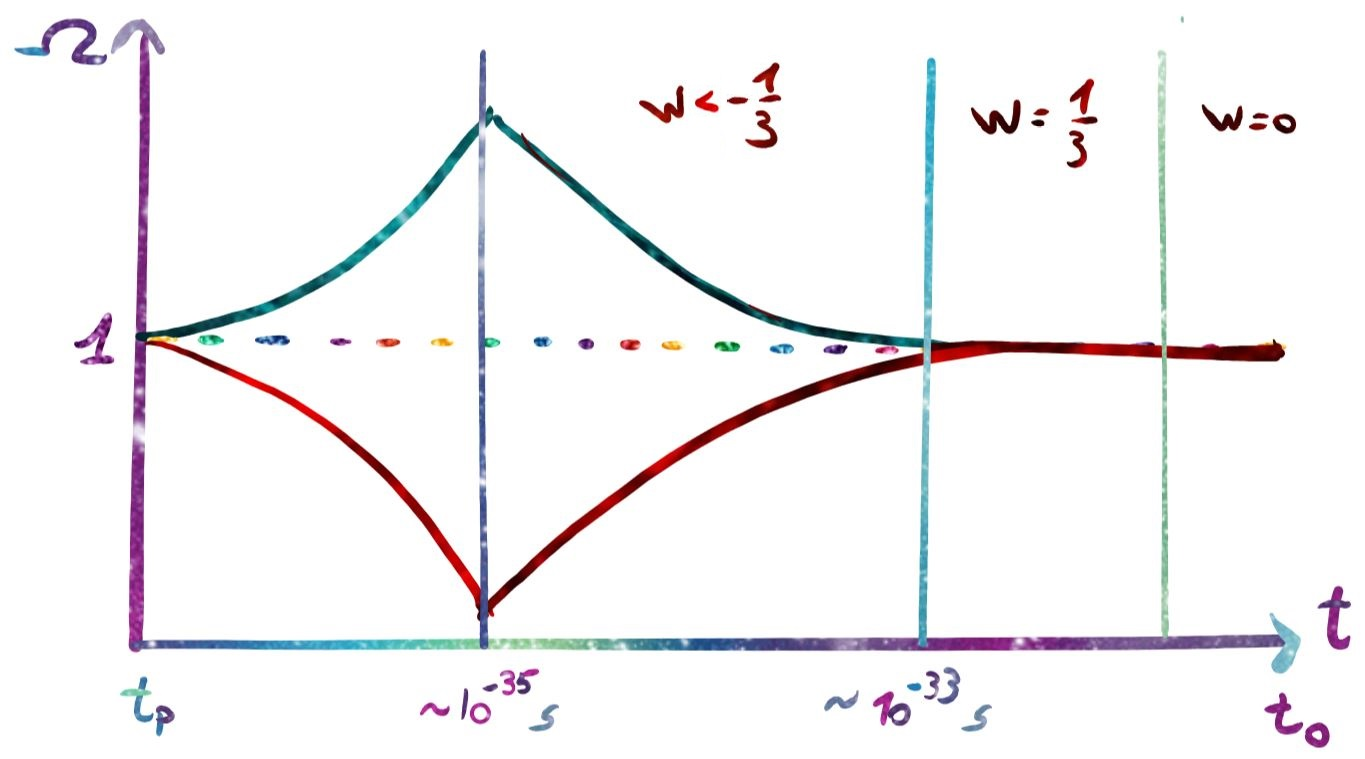
\includegraphics[width=.75\textwidth]{Pictures/4/omegainflation.jpg}
    \caption{Evoluzione di $\OmegaTOT$ per universi chiusi (linea verde), aperti (linea rossa) e piatti (linea tratteggiata arcobaleno). Durante il periodo inflazionario il valore del parametro di densità si schiaccia talmente tanto a $1$, che oggi è ancora lì.}
\end{figure}

\vspace{1em}
\noindent Morale, il problema dell'età (della piattezza) è quindi risolto se:
\begin{itemize}
    \item $N_{ef} \ge 60$ (condizione meno stringente della precedente);
    \item Si trova una giustificazione fisica per questa soluzione matematica.
\end{itemize}


\section{Problema dei monopoli magnetici}
In base alla Teoria della Grande Unificazione (GUT) esiste un tempo dell'universo prima del quale la forza elettrodebole e la forza forte erano unificate, inoltre ci si aspetta che, così come esistono le cariche fondamentali del campo elettrico, esistano anche quelle del campo magnetico (\textbf{monopoli magnetici}). Una carica fondamentale è espressa in unità di carica di Dirac:
\begin{equation*} 
    g_n = n g_0 \qquad g_0 = 68.5 e = \frac{\hslash c}{2e}
\end{equation*}
La massa che dovrebbe corrispondere ai monopoli magnetici è espressa in unità di masse corrispondenti all'energetica della transizione GUT ($m_{GUT}\simeq 10^{14\div 15}$ GeV):
\begin{equation*} 
    m_{MM}\simeq 10^2 ~m_{GUT} \simeq 10^{16}\; \mathrm{GeV}
\end{equation*}

La creazione dei monopoli magnetici deve avvenire all'interno dell'orizzonte, per cui si può stimare la loro densità: $n_{MM}(t_{GUT})\ge 10^{-10} ~n_\gamma(t_{GUT})$. Al momento non sono stati trovati processi fisici che possano variare il rapporto $n_{MM}/n_\gamma$ (simile a $n_b/n_\gamma$), ma ad oggi sono stati osservati 0 monopoli magnetici.

Inoltre il parametro di densità dei monopoli magnetici dovrebbe valere:
\begin{equation*}
    \Omega_{MM,\, 0} = \frac{n_{MM,\, 0} ~m_{MM}}{\rho_{\mathrm{cr},\, 0}} \approx \Omega_{0b}\frac{m_{MM}}{m_p}\approx \Omega_{0b} \cdot 10^{16}
\end{equation*}
e genererebbe quindi un universo chiusissimo.

\vspace{1em}
\noindent Morale, la teoria GUT per descrivere l'universo primodiale prevederebbe anche:
\begin{itemize}
    \item Una densità attuale di monopoli magnetici simile a quella dei barioni (vs. osservazioni);
    \item Un valore attuale di $\OmegaO$ esagerato.
\end{itemize}
Anche in questo caso l'inflazione potrebbe risolvere il problema diluendo sufficientemente i monopoli magnetici da renderli oggi insignificanti.

\newpage
\section{Problema della Costante Cosmologica}
Osservando l'espansione accelerata dell'universo ($q_0=-0.55$) si ha un'evidenza passiva della costante cosmologica. Il problema fisico risiede nel fatto che, prendendo dalle osservazioni $\Omega_{0\Lambda}$, si ottiene un valore estremamente piccolo $\Lambda\simeq 10^{-55}$ cm$^{-2}$. La massa associata a tale campo sarebbe:
$$
m_\Lambda = \left( \frac{\rho_\Lambda ~\hslash^3}{c^3}\right)^{1/4} \le 10^{-32}\; \mathrm{eV}
$$
che è una quantità estremamente bassa. La costante cosmologica può essere interpretata associandola all'energia del vuoto. Nel caso in cui avvenga una transizione di fase, parte dell'energia del vuoto ($\Delta \rho_V \sim m^4 c^3 / \hslash^3$) può essere estratta per generare la nuova fase ordinata.

\subsubsection{Energia del vuoto al tempo di Plank}
Si ottiene risommando tutta l'energia spesa nelle diverse transizioni di fase (Capitolo \ref{5:ch}):
$$
\rho_V (t_P) = \rho_V (t_0) + \sum_{jumps} \frac{m_i^4}{(\hslash / c)^3}= \left(\sum_{jumps}\Delta\rho_V \right) \left ( 1 + 10^{-108}\right)\; \mathrm{GeV^4}
$$
Anche in questo caso si è di fronte a un problema di fine-tuning, ossia il vuoto aveva moltissima energia e ha perso $108$ ordini di grandezza che però non possono essere posti a $0$ altrimenti non ci sarebbe $\Lambda$ oggi. Inoltre ci si chiede come mai la costante cosmologica abbia un contributo non trascurabile solamente oggi e, per non essere antropocentrici, questo è un problema di coincidenza che può essere alleggerito con $w<-1/3\neq -1$ spostando indietro nel tempo il momento in cui $\rho_\Lambda=\rho_m$ (modelli di quintessenza). 

\vspace{1em}
\noindent Morale, l'introduzione della costante cosmologica porta a:
\begin{itemize}
    \item Un problema di fine tuning dell'energia del vuoto;
    \item Un problema di coincidenza.
\end{itemize}
In generale il problema della costante cosmologica non ha soluzione.


\section{Transizioni di Fase}
La transizione di fase è il passaggio di un sistema fisico da uno stato d'ordine zero (disordine) ad un altro diverso da zero. (e.g. materiali ferromagnetici per i quali $\vec{B}\neq 0$ nel momento in cui si scende sotta la temperatura di Curie). L'energia libera è definita come la differenza tra l'energia interna e l'entropia: $F=U-TS$. Un sistema tende sempre a raggiungere il minimo di energia, una posizione stabile (e avere molta entropia aiuta). In particolare si analizzano i comportamenti di:
\begin{equation}
    F=F_0 +\alpha \phi^2 + \beta \phi^4 + \gamma (\phi^2)^{3/2}
\end{equation}
dove $\phi$ è un genetico \textit{parametro d'ordine} che dipende dalla temperatura. Questa forma di $F$ si basa sull'assunzione che esista un qualche tipo di simmetria ($F=F(\phi^2)$).


\begin{example}[Transizione del secondo ordine]
    $\beta > 0 \quad \gamma = 0 $
\end{example}
Nel caso in cui $\alpha >0$ si ha una forma parabolica con un minimo sull'asse y, mentre per  $\alpha <0$ si hanno due minimi assoluti simmetrici e un massimo relativo sull'asse y. Si può assumere che $\alpha$ dipenda dalla temperatura: $\alpha =a(T-T_c)$, dove $a$ è una costante e $T_c$ la temperatura critica della transizione di fase. Al calare della temperatura si ha la situazione illustrata in Figura \ref{fig4:transfase}. Il sistema si posizionerà in uno dei due nuovi minimi istantaneamente e in modo graduale ($\Delta F = 0$ in un tempo infinitesimo).

\newpage
\begin{example}[Transizione del primo ordine]
    $\beta > 0 \quad \gamma < 0 $
\end{example}
In questo caso, nel momento in cui si scende sotto la temperatura critica, la forma di $\phi$ non permette una transizione istantanea e graduale. Quando avviene la fluttuazione statistica che dà inizio alla transizione di fase si ha $T \ll T_c$, motivo per cui nella transizione viene rilasciato del calore latente ($\Delta F \neq 0$ in un tempo finito).

\begin{figure}[ht]
    \centering
    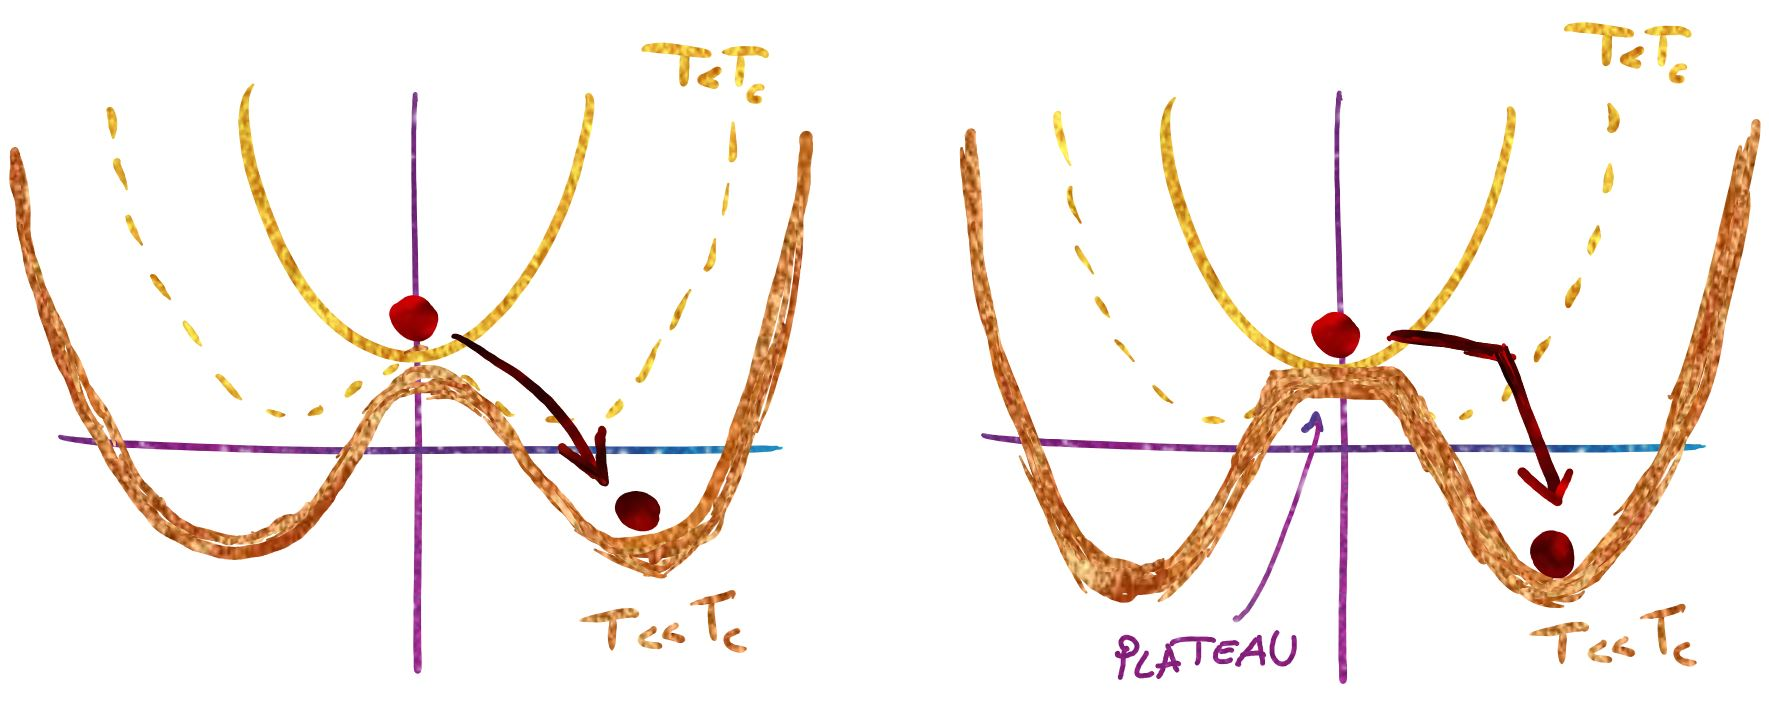
\includegraphics[width=.85\textwidth]{Pictures/4/transfase.jpg}
    \caption{Transizioni di fase del secondo (sinistra) e primo (destra) ordine.}
    \label{fig4:transfase}
\end{figure}



\noindent Le transizioni di fase che ha vissuto il nostro universo sono cronologicamente:
\begin{itemize}
    \item \textbf{GUT}: disaccoppiamento forza elettrodebole (leptoni) e forza forte (adroni). Questa è la transizione che più di tutte "svuota il vuoto" e avviene a $10^{15 }$ GeV;
    \item \textbf{EWT}: disaccoppiamento forza debole e forza elettromagnetica ($10^{2}$ GeV);
    \item \textbf{QAT}: transizione quark-adrone ($0.2 \div 3$ GeV).
\end{itemize}
Inoltre, la teoria delle supersimmetrie prevederebbe un'ulteriore transizione di fase la cui scala è ancora oggetto di studio. 

Le condizioni di esistenza di una particella sono legate alla relazione:
$$
mc^2 < k_B T
$$
al passare del tempo $T$ diminuisce e, a causa di annichilazioni, sopravvivono soltanto particelle di massa via via minore e il loro livello di interazione è descritto da una sezione d'urto via via differente. L'equilibrio termico sarà raggiunto ogni qualvolta $\tau_{coll}\ll H^{-1}$ e questo è verificato sicuramente nelle fasi primordiali poiché la materia è relativistica. Quando la condizione di equilibrio è verificata si può scrivere:
\begin{equation}
    n_i = \frac{g_i}{2\pi^2}\left ( \frac{k_B T}{\hslash c} \right )\int \frac{x^2 \mathrm{d}x}{e^x \pm 1} = \binom{3/4}{1} \frac{g_i}{\pi^2}~\xi (3)~T^3
\end{equation}
dove $g_i$ rappresenta il peso statistico della particella $i$-esima, $\xi (3) \approx 1.2$ e i valori $\pm$ e soprasotto si applicano rispettivamente alle particelle di tipo fermionico e bosonico. Per la densità di energia si ha:
\begin{equation}
    \rho_i c^2= \binom{7/8}{1} \frac{g_i}{2}~\sigma ~T^4
\end{equation}
Questa relazione può essere utilizzata per modellare il fluido primordiale introducendo il peso statistico effettivo $g^*$, che descrive tutte le particelle accoppiate alla radiazione:
\begin{equation}
    \rho(T)c^2 = g^* ~ \frac{\sigma ~ T^2}{2} \qquad g^* = \sum g_{iB} + \frac{7}{8} \sum g_{iF} \label{eq:statisticweight}
\end{equation}
Oggi nulla è accoppiato alla radiazione: $g^*=2$ (bosoni), in passato $g^*>2$. Per valutare l'equilibrio potrebbe essere necessario includere altri contributi alla densità (e.g. $\rho_{dec}$, $\rho_{nRel}$, $\rho_{nTh}$), che sono però trascurabili nelle fasi iniziali.
\chapterimage{/5/head.jpg} % Chapter heading image
\chapter{Storia Cronologica dell'Universo}\label{5:ch}

Non ci si avventurerà nella selva oscura della teoria GUT, ma verranno soltanto citati graficamente i fenomini-chiave e i principali periodi che caratterizzano le primissime fasi di vita del nostro universo. A partire dal tempo di Plank, $t_P=10^{-43}$ s, gli effetti quantistici diminuiscono col passare degli istanti, ma leptoni e adroni sono ancora la stessa cosa. Per questo motivo in questa fase può essere violata la conservazione del numero barionico ($n_b + n_{\overbar{b}}$). Possono cioè verificarsi reazioni che ristabiliscano l'equilibrio in seguito a qualsivoglia deviazione da esso: $n_b = n_{\overbar{b}}$. La transizione GUT è l'unico momento in cui può essersi formata l'anisotropia di 1 parte su $10^8$ barioni (i modelli di bariogenesi faticano ancora a trovare un valore così piccolo). Inoltre in questi istanti si formano le cariche, tra cui i monopoli magnetici. Durante la fase intermedia successiva, che dura $10^{26}$ secondi, la temperatura cala di $12$ dex e alla fine si ha $R_H = 1$ cm. La fisica delle particelle fatica a trovare candidati per questo range di temperature, per questo il periodo viene definito \textit{deserto di particelle}. La seconda transizione importante è quella elettrodebole, durante la quale i leptoni e il neutrino possono prendere massa. Infine all'ultima transizione quark-adroni si ha $R_H = 1$ km. 

\begin{figure}[H]
    \centering
    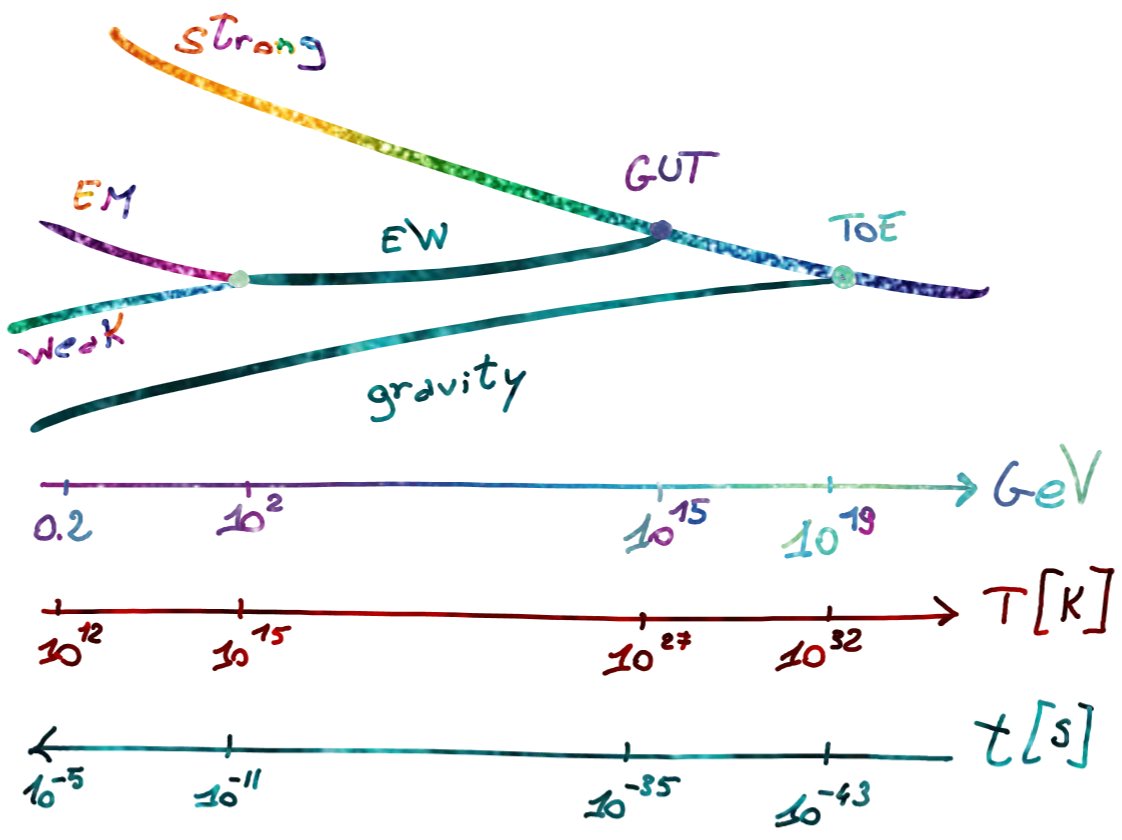
\includegraphics[width=.75 \textwidth]{Pictures/5/fasiprimordiali.png}
    \label{fig:4}
\end{figure}


\section{Modello di Guth (\textit{old inflation})}
I primo modelli di inflazione (anni `80) si basavano sulla teoria delle transizioni di fase del primo tipo. La temperatura critica precedentemente definita, è in questo caso la temperatura della transizione GUT e $\phi$ viene chiamato \textbf{inflatone}. A $T=T_{GUT}$ si iniziano a sviluppare due nuovi minimi allo stesso livello del vecchio e si viene quindi a creare una posizione di falso equilibrio o \textit{falso vuoto}. Al calare della temperatura il sistema non raggiunge istantaneamente la posizione di equilibrio a causa della barriera di potenziale dovuta alla forma di $\phi$. Quando la barriera di potenziale viene vinta il sistema è sovra-raffreddato e, raggiungendo il nuovo equilibrio, libera il calore latente (\textbf{reheating}). È quest'ultimo processo che può spiegare la generazione e termalizzazione di un grande numero di particelle.

La densità di lagrangiana dell'inflatone è: $\mathcal{L}_\phi = 1/2 \dt{\phi}^2-V(\phi, T)$ dove $V(\phi, T)$ è il potenziale che corrisponde al campo scalare dell'inflatone e fa il gioco dell'energia libera. Il contributo dell'inflatone al tensore energia-impulso vale:
\begin{equation*}
    T \phi_{ij}=-p_\phi g_{ij}+(p_\phi -\rho_\phi)~u_i u_j \qquad \left\{
        \def\arraystretch{1.5}
            \begin{array}{ll}
                p_\phi = \mathcal{L}_\phi = \frac{1}{2}\dt{\phi}^2-V \\
                \rho_\phi = \frac{1}{2}\dt{\phi}^2+V 
        \end{array}\right.
\end{equation*}
Dall'equazione di Eulero-Lagrange si trova l'\textit{equazione fondamentale della dinamica dell'inflatone}:
\begin{equation}
    \ddt{\phi} + 3H \dt{\phi} + \frac{\partial V}{\partial \phi} =0
\end{equation}
in cui $3H\dt{\phi}$ gioca il ruolo di termine di frizione. Il ``moto'' dovrà essere rallentato affinché l'inflazione duri a sufficienza. Includendo questi contributi nelle equazioni di Friedmann (ponendo $c=1$), si può verificare che l'espansione risultante è accelerata:
\begin{equation*}
\left( \frac{\dt{a}}{a}\right)^2 = \frac{8\pi}{3}G\rho_\phi \qquad \rho_\phi \simeq V \qquad \rightarrow \qquad a=a_0 ~e^{t/\tau} \qquad \tau^{-1} = \sqrt{8\pi G V /3}
\end{equation*}
Inoltre, assumendo un valore del potenziale $V$ si può calcolare il numero di e-folding:
\begin{equation*}
N_{ef} = -8\pi G \int_{\phi_i}^{\phi_f} \left(\frac{\mathrm{d} \ln V}{\mathrm{d}\phi}\right)^{-1}\mathrm{d}\phi
\end{equation*}
che cresce, ovviamente, quanto più è piatto il potenziale. 

Il problema di questi modelli è che prevedono una dimensione di $R_H$ insufficiente per coprire l'intero universo, si creano delle ``bolle di universo'' troppo piccole. Si è quindi passati a considerare le transizioni del secondo tipo, nonostante non offrano le possibilità di un rilascio di energia sotto forma di calore latente. Queste transizioni prevedono un inizio istantaneo dell'inflazione, quindi la forma del potenziale dovrà essere regolata in modo tale che l'inflazione duri a sufficienza. Anche tali \textbf{new inflation models} non sono stati apprezzati perché richiedono un \textit{fine-tuning} dei parametri.

\section{Modello di inflazione caotica}
Il paradigma attuale dell'inflazione, l'inflazione caotica, è dovuto a Linde e non si basa sulle transizioni di fase. È sufficiente che esista un campo scalare estremamente energetico e statico nella fase iniziale, $\phi$. L'equazione della dinamica, la densità e la pressione dell'inflatone sono le stesse.
\subsection{Potenziale quadratico}
Per semplificare i conti si utilizzano le unità planckiane (\ref{eq:unitaplanckiane}) e si assume un potenziale della forma:
$$
V(\phi)= \frac{m^2~\phi^2}{2}
$$
dove $m$ è la massa dello scalare corrispondente all'inflatone. L'equazione della dinamica dell'inflatone diventa:
\begin{equation}
    \ddt{\phi} + \sqrt{12 \pi} \left( \dt{\phi}^2+m^2 \phi^2 \right) \dt{\phi} + \frac{\partial V}{\partial \phi} =0
\end{equation}

Questa può essere studiata nello spazio delle fasi ($\phi, \dt{\phi}$) ed essendo del II ordine non autonoma vale la relazione $\ddt{\phi} = \dt{\phi} ~ \mathrm{d} \dt{\phi} /\mathrm{d} \phi$. Partendo con la condizione in cui il termine cinetico domina su quello potenziale, la traiettoria può essere studiata in tre fasi principali: caduta sull'attrattore, inflazione e graceful exit (Fig. \ref{fig5:chaotic}).

\vspace{1em}
\begin{example}[Caduta sull'attrattore] $\dt{\phi}^2 \gg m^2 \phi^2 \qquad p_\phi = \rho_\phi = \frac{\dt{\phi}}{2} \rightarrow w=1$ (\textit{ultra hard equation of state})
\end{example}
\noindent A differenza dei modelli visti in precedenza non è richiesto un particolare \textit{fine-tuning} dei parametri, ma si parte da generici valori iniziali $\dt{\phi} \gg \phi$. Dall'equazione della dinamica modificata si può ottenere l'andamento delle traiettorie in questo primo regime:
\begin{equation}
    -\dt{\phi} \frac{\mathrm{d} \dt{\phi}}{\mathrm{d} \phi} = \sqrt{12 \pi} \dt{\phi}^2 \quad \rightarrow \quad \dt{\phi} \propto e^{\sqrt{12 \pi} \phi}
\end{equation}
Integrandole in funzione del parametro tempo $t$:
\begin{equation}
    \phi= cost - \frac{\ln t}{\sqrt{12 \pi}} \qquad \dt{\phi} = \frac{1}{\sqrt{12 \pi}}\frac{1}{t};
\end{equation}
da cui è chiaro che in questa fase la traiettoria è praticamente parallela all'asse $\dt{\phi}$ ($\delta \phi \ll \delta\dt{\phi}$ ). Dalle equazioni di Friedmann si può inoltre verificare che l'andamento dei principali parametri cosmogici è lo stesso di un universo EdS con $w=1$:
\begin{equation}
    H = \frac{1}{3t} \qquad a \propto t^{1/3} \qquad \rho \propto a^{-6}
\end{equation}

In conclusione, se il campo scalare parte con un'energetica sufficiente, il sistema raggiunge naturalmente un $\phi$ poco differente dal valore iniziale a seguito di una forte diminuzione di $\dt{\phi}$.

\vspace{1em}
\begin{example}[Inflazione] 
    $\mathrm{d} \dt{\phi} / \mathrm{d} \phi=0 \qquad m\phi_i \gg \dt{\phi}_i$
\end{example}

Queste due assunzioni sono finalizzate al risultato finale, ossia quello di avere una fase inflazionaria sufficientemente lenta, in particolare è richiesto che il valore di inserzione $\phi_i$ sul cosiddetto \textbf{attrattore} sia sufficientemente alto. 
\begin{equation}
    \dt{\phi} =  -\frac{m}{\sqrt{12 \pi}} = cost \qquad \phi= \phi_i - \frac{m}{\sqrt{12 \pi}} (t-t_i) = \phi_f - \frac{m}{\sqrt{12 \pi}} (t-t_f); \label{eq:phidotphiinfl}
\end{equation}

Si assume $\phi_f = 0$, per cui il valore del potenziale sull'attrattore è $V= m^4 (t_f-t)^2 / 24 \pi$. L'inflazione termina quando $\ddt{a}=0$, ossia $\rho_\phi = -3p_\phi = m^2 / 8 \pi$. Dato che in questo regime $\rho_\phi \approx V$ si ha:
$$
\phi_f = \sqrt{\frac{1}{4\pi}}= \mathcal{O}(1)
$$
Il potenziale alla fine di questa fase è quindi dell'ordine di 1 volta il potenziale al tempo di Planck. Dalle equazioni di Friedmann si può inoltre calcolare l'andamento dei principali parametri cosmogici:
\begin{equation}
    H^2 = \frac{8\pi }{3}\rho_\phi \rightarrow H = \frac{m^2}{3} (t_f -t) \qquad a=a_f e^{-m^2 (t_f-t)^2 /6} \qquad a=a_i e^{(H+H_i)(t-t_i)^2 /2}
\end{equation}
Si nota che $H$ descresce in modo lineare nel tempo, mentre $a$ si espande in modo esponenziale: \textbf{inflazione}. Per risolvere i problemi dell'età dell'universo e dell'orizzonte si applica la condizione $\ln (a_f/a_i) \gg 60$ assumendo $\phi_f = 0$ e utilizzando l'equazione (\ref{eq:phidotphiinfl}):
\begin{equation}
    2 \pi \phi_i^2 \gg 60 \quad \rightarrow \quad \phi_i \gg 3 \div 4
\end{equation}
Questo significa avere valori di $\phi$ più grandi di quelli al tempo di Planck, ma la fisica è dettata da $V$. La condizione per non dover includere anche effetti quantistici è $V_i<1$, ossia: $m^2 \phi_i^2 /2 <1$. A $m=m_{GUT}$ si deve avere $\phi_i < 10^4$ unità plankiane: la condizione su $\phi_i$ può quindi essere valida.

\vspace{1em}
\begin{example}[Graceful Exit] 
    $H^2=\frac{4\pi }{ 3} \left(\dt{\phi} +m^2\phi^2\right) \qquad \ddt{\phi} + 3H \dt{\phi} + \frac{\partial V}{\partial \phi} =0$
\end{example}
In questa fase si utilizzano tutti i termini dell'equazione della dinamica. Dalla prima equazione: 
\begin{equation}
    \dt{\phi} \equiv \sqrt{\frac{3}{4\pi}} ~H \sin \theta, \quad m\phi \equiv \sqrt{\frac{3}{4\pi }} ~H \cos \theta
\end{equation}
dove $\theta$ rappresenta l'angolo che descrive la traiettoria nello spazio ($\dt{\phi}, m\phi$). Derivando temporalmente le quantità $(H\sin\theta)$ e $(H\cos\theta)$ si ottengono le relazioni:
\begin{equation}
    \dt{H} = -3H^2 \sin^2 \theta \qquad\qquad  \dt{\theta} \propto -m \qquad \theta \propto -mt
\end{equation}
La derivata del parametro di Hubble oscilla nel tempo, ma è smorzata all'aumentare di H e l'angolo di fase varia linearmente. Integrando nel tempo si può ottenere il valore di $H$ e $a$ per $mt$ piccoli:
\begin{equation}
    H = \frac{2}{3t}\left( 1+ \mathrm{sinc} (2mt)\right) + \mathcal{O}(t^{-3}) \qquad\qquad a\propto t^{2/3}
\end{equation}
La $\mathrm{sinc}$ smorza l'ampiezza della spirale di H. Questo risultato non ci soddisfa particolarmente, perché usciremmo dall'inflazione con un'equazione di stato che non corrisponde alla componenete radiativa ($a_{EdS}\propto t^{1/2}$). Lo smorzamento sarà comunque il meccanismo che genererà le fluttuazioni di inflatone (particelle).


\begin{figure}[H]
    \centering
    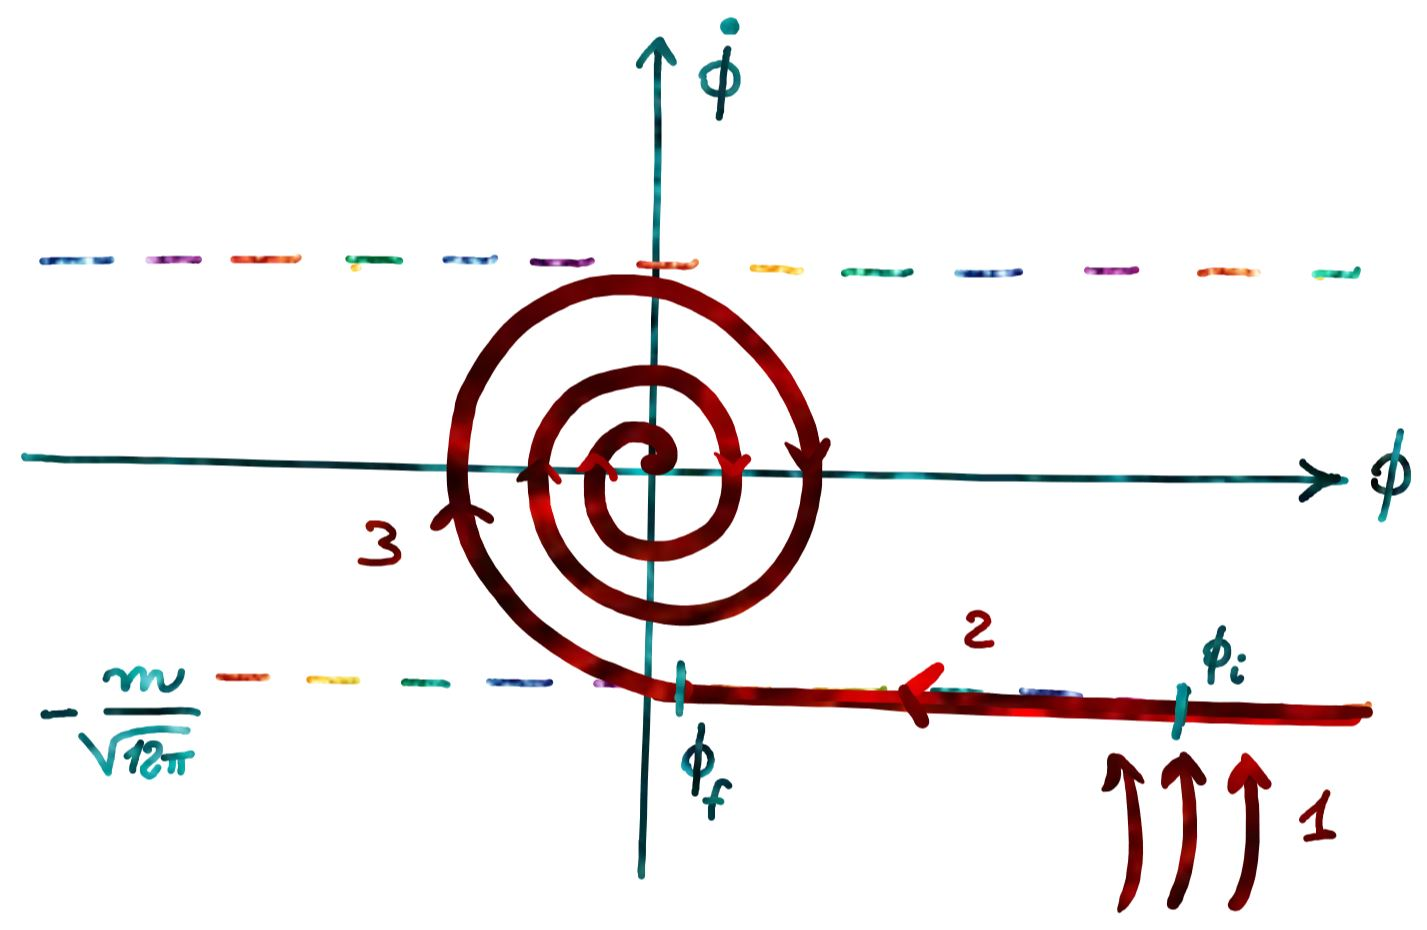
\includegraphics[width=.9 \textwidth]{Pictures/5/chaosinfl.jpg}
    \caption{Diagramma di fase per il modello di inflazione caotica. Si distinguono le tre fasi principali: (1) caduta sull'attrattore, (2) inflazione, (3) graceful exit. Per il potenziale quadratico si ha: $\phi_i\gg  4$ e $\phi_f = \mathcal{O} (1)$. Comportamenti speculari si avrebbero partendo dal secondo quadrante.}\label{fig5:chaotic}
\end{figure}


\subsection{Potenziali generalizzati}\label{ch5:epsieta}
Per forme del potenziale diverse da quella quadratica (bocciata dal satellite Plank) valgono comunque le equazioni:
\begin{equation*}\left\{
    \def\arraystretch{1.5}
        \begin{array}{ll}
            \ddt{\phi} + 3H \dt{\phi} + \frac{\partial V}{\partial \phi} =0\\ 
            H^2 = \frac{8\pi}{3} \left(\dt{\phi}^2+V\right)
    \end{array}\right.
\end{equation*}

Per risolvere i problemi dell'orizzonte e della piattezza si introducono le condizioni di lento rotolamento (\textbf{slow roll}):
\begin{equation}
    \left| \dt{\phi}^2 \right| \ll \left| V \right|  \qquad\qquad \left| \ddt{\phi} \right| \ll \left| 3H\dt{\phi} \right|;
\end{equation}
che corrispondono rispettivamente alle richieste che il termine potenziale sia dominante rispetto a quello cinetico e l'accelerazione domini sul termine di frizione. In questo modo si ottiene $a'/a = -8\pi V/V'$ (l'apice indica la derivata rispetto a $\phi$), da cui:
\begin{equation}
    60 \ll N_{ef} = 8\pi \int_\phi^{\phi_i} \frac{V}{V'} \mathrm{d}\phi. 
\end{equation}
In letteratura le condizioni di slow rolling vengono riscritte sotto forma di $V'$ e $V''$:
\begin{equation}
    \left| \left( V'/V\right)^2 \right| \ll 1 \qquad\qquad \left|  V''/V \right| \ll 1;
\end{equation}
e vengono introdotti i seguenti parametri:
\begin{equation}
    \varepsilon = \frac{1}{16\pi}\left(\frac{V'}{V}\right)^2 \qquad\qquad \eta = \frac{1}{8\pi}\left|\frac{V''}{V}\right|^2
\end{equation}
In generale bisogna avere $\varepsilon, \eta \ll 1$ (in unità planckiane), ma i valori precisi vengono calcolati per ogni nuovo modello, perché lasciano caratteristiche osservabili sulla CMB e nella struttura a larga scala (deviazioni dalla perfetta gaussianità). In pratica l'inflazione è falsificabile attraverso questi due numeretti. Un potenziale a legge di potenza $V=\lambda \phi^n / n$ ha le seguenti caratteristiche:
\begin{equation}
    \varepsilon =   \frac{1}{16\pi} \left( \frac{n}{\phi}\right)^2 \qquad \eta= 2 \frac{n-1}{n} ~\varepsilon \qquad\qquad a(\phi)=a_i ~e^{N_{ef}} = a_i ~e^{4\pi(\phi_i^2-\phi)/n}
\end{equation}
ossia restituisce sempre un'espansione esponenziale che può essere regolata tramite $n$ per ottenere l'$N_{ef}$ desiderato.

\subsection{Reheating}
La termalizzazione è possibile grazie all'elevata quantità di energia disponibile e può essere legata al decadimento dell'inflatone. Questo processo può avvenire in due modi:
$$
\phi \rightarrow \chi + \chi \qquad \phi \rightarrow \psi + {\overbar{\psi}}
$$
nel primo caso viene prodotta una coppia di scalari e nel secondo una coppia fermione-antifermione. La lagrangiana di interazione è $\Delta \mathcal{L} = -g \phi \chi^2 - h \phi \psi {\overbar{\psi}}$ dove $g$ e $h$ sono le costanti di accoppiamento dei due processi. I rispettivi tassi di decadimento sono dati dalle seguenti relazioni:
$$
\Gamma_\chi = g^2 / 8\pi m \qquad \Gamma =h^2 m / 8\pi 
$$
Per evitare di entrare nel regime quantistico bisogna che $g \lesssim m$ e $h\lesssim m^{1/2}$, quindi si possono assumere $\Gamma_\chi \approx m$ e $\Gamma_\psi \approx m^2$. Per cui a $m_{GUT}=10^{-4}$ si ha $\Gamma_\psi \ll \Gamma_\chi$ e domina il processo di decadimento degli scalari. La variazione di densità numerica degli scalari seguirà quindi la legge: $\dt{n}_\phi = - g^2 ~n_\phi / 8\pi m$. Il numero di oscillazioni dello scalare inflatone nell'unità di tempo (``giri di spirale'') è: $N_{osc}=mt/2\pi$, per cui passando per il differenziale $\mathrm{d}n_\phi$ si ha:
\begin{equation}
    n_\phi \propto e^{-g^2 ~N_{osc}/4m^2}
\end{equation}
Sostituendo $g \sim m$ sono sufficienti pochissime oscillazioni per far decadere tutti gli inflatoni e formare gli scalari $\chi$. Anche per $g \ll m$ questo è verificato, grazie al contributo di processi di risonanza e condensazioni di Bose. Inoltre, assumendo che la massa dell'inflatone sia $m=10^{13}$ GeV ($10^{-6}$ unità planckiane):
\begin{equation}
    n_\phi (t_f)\approx \frac{1}{2}m\phi_f^2 \approx 10^{92}\; \mathrm{cm^{-3}}
\end{equation}
si ottengono un sacco di particelle e tutta l'entropia che potrebbe servire. Oggi l'energia dell'universo è talmente bassa che processi come questo non possono avere luogo, l'inflazione va collocata a livelli energetici alti.

\subsubsection{Temperatura di Reheating}
La temperatura in uscita del processo di inflazione deve necessariamente essere $T_{RH}<T_{GUT}\simeq 10^{16}$ GeV, altrimenti si riattraverserebbe ciclicamente la transizione GUT (pb. monopoli magnetici e cose di questo tipo). In ogni caso è necessario termalizzare l'universo, ossia $\Gamma_\chi^{-1}<H^{-1}$, nel limite in cui si equivalgono (corrispondente alla fine del processo) si ha:
\begin{equation}
    \Gamma_\chi \simeq \frac{m}{8\pi} \quad\equiv\quad H \simeq \sqrt{\frac{8\pi^3}{90}g^* T^4}\quad \rightarrow \quad T_{RH} = 2\cdot 10^{-4} \left( g^*_{100} \right)^{-1/2} \left( m_{\phi, -6} \right)^{1/2}
\end{equation}
La cosiddetta temperatura di reheating dipende quindi dalla massa dell'inflatone, nel caso in cui $m_\phi = 10^{-6}$ si avrebbe $T_{RH}\approx 10^{-4}\;\mathrm{T_P}=10^{15}$ GeV che è già pericoloso! 

\newpage
\subsubsection{Sommario}
Il paradigma dell'inflazione si aggiunge al modello del Big Bang per risolvere tre dei cinque problemi: orizzonte, piattezza e monipoli magnetici. Il problema dell'orizzonte si ha perché vediamo la connessione causale su regioni dell'universo che sono più grandi della regione dell'orizzonte e viene risolto assumendo che la connessione causale era stata raggiunta già prima. Il problema della piattezza si riferisce a una richiesta di perfetto bilanciamento tra energia cinetica e potenziale. Inoltre il modello del Big Bang prevederebbe oggi un'alta densità di monopoli magnetici che avrebbero dovuto chiudere immediatamente l'universo e comunque non sono stati osservati. I primi due problemi possono essere risolti mediante un'espansione accelerata dell'universo che inverte i comportamenti del raggio dell'orizzonte e del parametro di densità totale. La durata di questa espansione deve comunque essere sufficientemente lunga: la condizione richiesta dal primo problema $N_{ef} \gg 60$, soddisfa pienamente anche il secondo. 

Storicamente i primi modelli si sono appoggiati alle transizioni di fase perché avvengono all'energetica richiesta e generano le particelle desiderate. La dinamica è descritta dall'equazione fondamentale dell'inflazione che è derivata dall'equazione di Eulero-Lagrange per l'inflatone (parametro d'ordine delle transizioni di fase). Applicando le condizioni di slow rolling si ottengono: espansione accelerata e un numero sufficiente di e-folding. In particolare i modelli old inflation utilizzavano le transizioni del primo tipo, mentre quelli new inflation le transizioni del secondo tipo. Si è poi concluso che non funzionavano perché non riuscivano a generare regioni abbastanza grandi da contenere il nostro universo e richiedevano un fine-tuning dei parametri.

Il modello attuale è quello dell'inflazione caotica. La dinamica dell'inflatone, ora inteso come campo scalare estremamente energetico, è descritta dalla stessa equazione di cui sopra. In questo caso si può avere un ampio range di condizioni iniziali che generano quasi tutte la stessa traiettoria, infatti inizialmente le curve cadono sull'attrattore e da qui ha inizio l'inflazione (non è più richiesto un fine-tuning). Durante la fase di inflazione, $\phi_i \rightarrow \mathcal{O}(1)$, si ha espansione accelerata e si può avere l'$N_{ef}$ necessario purché $\phi_i \gg 3\div 4$. Inoltre la richiesta di non entrare in regime quantistico $V<1$ si traduce in un limite superiore a $\phi_i$. In conclusione, $ 3 \ll \phi_i < 10^4$ in unità planckiane. In questo modo si può stabilire quale valore (naturalmente al di sotto di $m_P$) associare alla massa dello scalare inflatone, e.g. $m_\phi = 10^{-6}$. Si può dimostrare che questo approccio vale anche per forme del potenziale $V$ leggermente diverse da quella quadradica. 

Quando si esce dalla fase di inflazione, $\phi = \mathcal{O}(1)$, si può innestare un meccanismo di decadimento dello scalare inflatone. La fisica delle particelle garantisce che il processo dominante è quello di decadimento in due scalari e anche pochi giri di spirale sono sufficienti per riempire l'universo di particelle. Inoltre, per avere $w=1/3$ in uscita, si può termalizzare l'universo purché la temperatura di reheating rimanga minore della temperatura GUT. Lo ``stiramento'' provocato dall'inflazione appiattisce l'universo e qualunque perturbazione ci sia in esso, all'uscita quindi l'universo è omogeneo e isotropo (\textit{cosmic no hair theorem}).

\vspace{1em}
\noindent Alcune predizioni dell'inflazione sono falsificabili: 
\begin{itemize}
    \item[-] $\Omega_{TOT} = 1$, universo piatto (confermato da Planck a meno di $10^{-2}$);
    \item[-] Le particelle generate creano fluttuazioni pressoché gaussiane nel campo di densità;
    \item[-] Distribuzione della scala angolare del campo di densità (pressoché \textit{scale invariant});
    \item[-] Piccole deviazioni da gaussianità e invarianza di scala legate a $\varepsilon \leftrightarrow  V' $ e $\eta \leftrightarrow V''$;
    \item[-] Fluttuazioni tensoriali (onde gravitazionali).
\end{itemize}

\vspace{1em}
In conclusione, l'inflazione non è un modello, è un paradigma, una famiglia di modelli che hanno in comune la richiesta di avere campi sufficientemente energetici. Si distinguono dall'avere predizioni diverse per $\varepsilon$, $\eta$ e onde gravitazionali. Con i dati di Plank una buona serie di modelli inflazionari è stata rigettata, ma ci sono ancora più modelli che teorici al mondo. Il vantaggio di studiare la CMB piuttosto che la LSS sta nel fatto che ha molta più memoria (perché è più temporalmente vicina) delle condizioni iniziali. 


\section{L’era adronica e l’era leptonica}
L'ultima delle grandi transizioni di fase, la transizione quark-adroni, avviene a $T=200\div 300$ MeV a circa $10^{-5}$ s. Da questo istante i quark si possono unire per dare origine agli adroni. 

\subsection{Era adronica}
Le reazioni che caratterizzano questo periodo sono quelle che trasformano adroni in fotoni (reazione di annichilazione) e viceversa e l'annichilazione dei tau. Quest'era è molto breve e termina nel momento in cui anche i pioni si annichilano, $T_\pi = 130$ MeV. Alla fine si avranno: leptoni, antileptoni, fotoni e protoni e neutroni in misura pari all'eccesso barionico. In particolare, dalla distribuzione di Boltzmann:
\begin{equation}
    n=2\left(\frac{mk_b T}{2\pi \hslash}\right)^{3/2}  e^{(\mu - mc^2)/{k_B T}} \label{eq:boltzmann}
\end{equation}
dove $\mu$ è il potenziale chimico che in questo caso, come in tutti i casi in cui si hanno particelle assieme ad antiparticelle, vale $0$ (conservazione carica, numero barionico e leptonico, carica dell'universo nulla). Da cui:
\begin{equation}
    \frac{n_n}{n_p}=\left(\frac{m_n}{m_p} \right)^{3/2}e^{-(m_n-m_p)c^2 / k_B T} \label{eq:nn-vs-np}
\end{equation}

Considerando che $(m_n-m_p)c^2=1.3$ MeV $\rightarrow 1.5\cdot 10^{10}$ K, per questo periodo si può assumere $n_n\simeq n_p$, questa approssimazione regge fintantoché $T\gg 1.3$ MeV. Conoscere questo rapporto nelle epoche successive è molto importante per modellare la nucleosintesi primordiale.


\subsection{Era leptonica}
Le reazioni che caratterizzano questo periodo sono quelle di produzione e di annichilazione di paia di leptoni. È un'era molto interessante perché permette di caratterizzare le proprietà dei neutrini e su di essa si fondano le condizioni iniziali della nucleosintesi primordiale. Ha inizio dal decadimento del pione ($10^{-5}$ s) e finisce quando si annichila l'elettrone ($10$ s, T=$0.5$ MeV). È caratterizzata da: leptoni ($e^-$, $e^+$, $\mu^-$, $\mu^+$, 3 neutrini), fotoni e l'eccesso barionico (trascurabile). Il peso statistico effettivo vale (\ref{eq:statisticweight}):
$$
g^* = 2 + \frac{7}{8}(4\cdot 2 + 3 \cdot 2) \simeq 14.25
$$
valore molto inferiore rispetto all'era di Planck $\approx 200$ e all'inflazione $\approx 100$. Si può verificare che il tempo tipico di interazione è molto più piccolo di $\tau_{exp}$ , per cui tutte queste particelle rimangono in equilibrio termico. Successivamente si annichilano $\mu^-$ e $\mu^+$ e infine $e^-$, $e^+$.

Qualsiasi annichilazione (e.g. $e^- + e^+ \leftrightharpoons \gamma + \gamma$) è un processo termodinamicamente reversibile che conserva l'entropia $S=(p+\rho c^2)V/T$ Considerando che tutto è accoppiato alla radiazione e che il volume cambia in modo trascurabile (dalla \ref{eq:statisticweight}, $S\propto T^3g^*$):
\begin{equation}
    S_{-} \equiv S_{+} \qquad \rightarrow \qquad T_+ = T_- \left(\frac{g^*_-}{g^*_+}\right)^{1/3} 
\end{equation} 
e dato che $g^*_+ < g^*_-$, la temperatura dell'universo cresce in seguito a ogni fase di annichilazione. Per i fotoni, essendo dall'era di Planck ad oggi $T: 10^{32}\rightarrow 2.7$ e $g^*: 200\rightarrow 2$, l'effetto è praticamente trascurabile, ma lascia una \textit{feature} importante per i neutrini.

\subsubsection{Disaccoppiamento dei neutrini}

L'accoppiamento dei neutrini con i leptoni può avvenire attraverso le seguenti reazioni elettrodeboli:
$$
\nu_e + \mu^- \leftrightharpoons {\overbar{\nu}_\mu} + e^- \qquad {\overbar{\nu}_\mu} + \mu^+ \leftrightharpoons \nu_e + e^+ 
$$
Confrontando il tempo di interazione $\tau_{coll}=(\sigma_{EW}~n_{lep}~c)^{-1}$ con il tempo di espansione dell'universo $H^{-1}_{w=1/3} = 2t$, si ha: 
\begin{equation}
    \frac{\tau_{exp}}{\tau_{coll}}= \left (\frac{T}{3\cdot 10^{10}\;\mathrm{K}}\right)^3
\end{equation}

Per cui a partire da $T= 3\cdot 10^{10}$ K si ha il disaccoppiamento dei neutrini. Questo avviene dopo l'annichilazione dei $\mu$, ma prima dell'annichilazione degli $e$. Ricapitolando, quando si annichila la coppia $\mu$: leptoni e fotoni sono accoppiati e fanno ambedue un salto in temperatura. Al momento del disaccoppiamento ($T=3\cdot 10^{10}$ K) i neutrini sono relativistici, così come i fotoni, quindi anche se non si parlano più hanno la stessa adiabatica. Al momento dell'ultima annichilazione, quella della coppia $e$ ($T=3\cdot 10^{9}$ K), soltanto la radiazione subisce un salto in temperatura dopodiché seguirà di nuovo l'andamento $a^{-1}$ (Fig. \ref{fig5:salti}). 


\begin{figure}[ht]
    \centering
    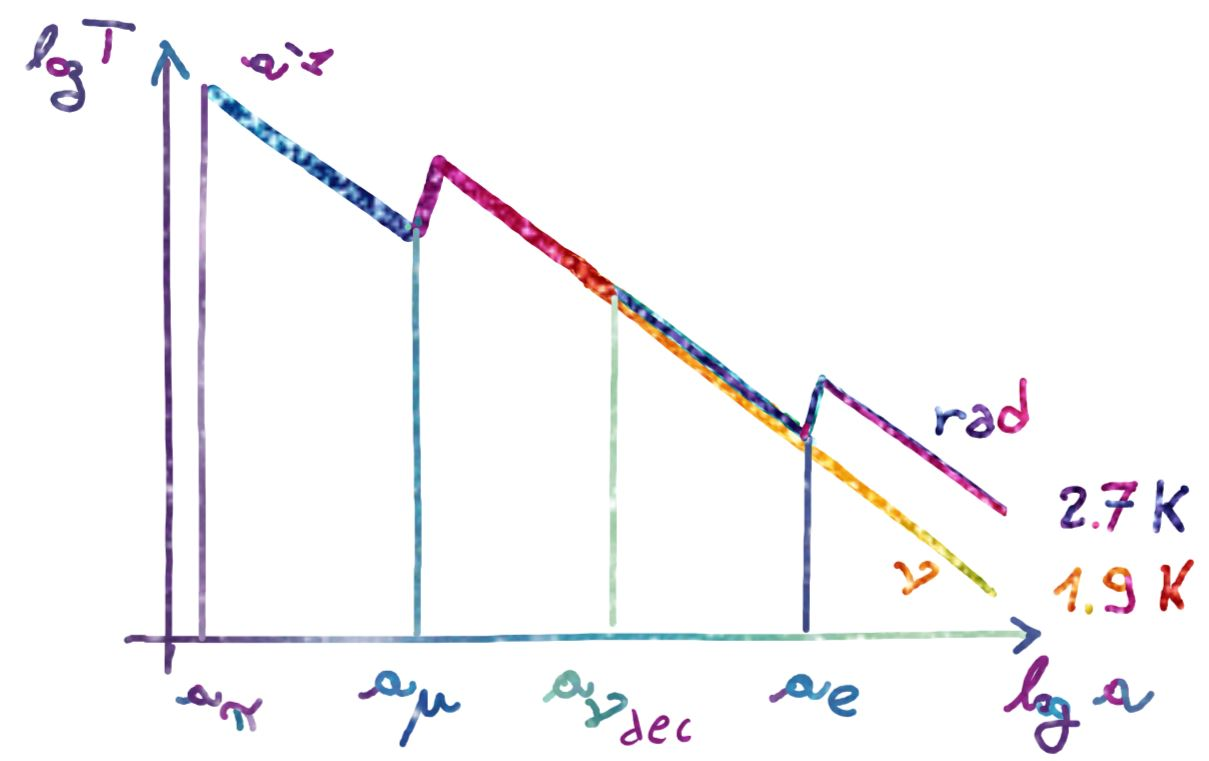
\includegraphics[width=.7 \textwidth]{Pictures/5/annichilazioni.jpg}
    \caption{Temperatura dal variare di $a$ in seguito a: decadimento del pione $a_\pi$, annichilazione dei muoni $a_\mu$, disaccoppiamento dei neutrini $a_{\nu_{dec}}$ e annichilazione della coppia elettrone-positrone $a_e$.}\label{fig5:salti}
\end{figure}


La differenza di temperatura tra radiazione e neutrini è mantenuta fino ad oggi:
$$
T_+ = T_- \left(\frac{11}{4} \right)^{1/3}\simeq 1.4 ~T_-
$$

La temperatura del neutrino oggi deve quindi essere:
$$
T_{\nu\, 0} \simeq \frac{T_{r\, 0}}{1.4} \simeq 1.9 \, \mathrm{K}
$$

Se il neutrino non ha massa (modello standard delle particelle), vale la relazione $\rho_\nu c^2 =\sigma T^4$, da cui si ottiene un contributo $\Omega_{\nu\, 0}\simeq 0.7 \Omegaro$ da aggiungere alla componente relativistica. 

Se il neutrino avesse massa $10$ eV (numero non a caso), si de-relativizzerebbe a $T\approx T_{eq,\, rad}$. In questo caso $T$ è una pseudo-temperatura, ma vale comunque la relazione $n_\nu \propto T_\nu^3$, che restituisce $n_\nu = 320$ cm$^{-3}$ (cfr. $n_\gamma=420$ cm$^{-3}$). Questa quantità contribuisce in questo caso alla componente di materia oscura. In particolare, assumendo che tutta la materia oscura sia dovuta ai neutrini, si può trovare un limite superiore alla loro massa media (tra i tre tipi):
$$
\left \langle m_\nu \right \rangle \le \frac{\Omegamo ~\rho_{cr}}{n_\nu} \qquad \rightarrow\qquad \left \langle m_\nu \right \rangle \le 10\, \mathrm{eV}
$$

In realtà si sa che il neutrino non ha le propietà che ci piacciono per rappresentare tutta la materia oscura (è troppo ``caldo'') e come si vedrà dovrà essere minore di qualche decimo di eV. 


\section{Nucleosintesi Primordiale}
I fenomeni che caratterizzano la nucleosintesi erano già studiati negli anni `40 in associazione con gli interni stellari e le bombe atomiche. È considerata una delle prove fondamentali a favore del modello del Big Bang perché riesce a spiegare molto bene le abbondanze degli elementi leggeri (ciò che le stelline del Prof. Ferraro non possono spiegare). In particolare può giustificare l'alta abbondanza di elio $Y=0.25$. Le condizioni cosmologiche impediscono la formazione di elementi più pesanti a causa delle elevatissime temperature, il problema sarà la formazione del deuterio (che è un collo di bottiglia). Inoltre il modello ha predetto l'esistenza di un fondo cosmico a $T=5$ K, scoperto 30 anni dopo. 

\vspace{1em}
\noindent Le assunzioni del modello standard della nucleosintesi primordiale sono:


\begin{table}[ht]
    \def\arraystretch{1.5}
    \begin{tabular}{lll}

    \textbf{1)} & $T\ge 10^{12}$ K $\quad$  (\textit{hot Big Bang}) \\
    \textbf{2)} & General Relativity $+$ Fisica delle Particelle \\
    \textbf{3)} & Universo sufficientemente Omogeneo e Isotropo  \\
    \textbf{4)} & Cinque o meno tipologie di neutrini \\
    \textbf{5)} & Neutrini non degeneri \\
    \textbf{6)} & Non esistono troppe regioni di antimateria \\
    \textbf{7)} & $\vec{H}$ trascurabili  \\
    \textbf{8)} & Non esistono particelle esotiche \\
    \end{tabular}
    \end{table}

Le condizioni di base sono (1), (2) e (3), in particolare la (3) è verificata con l'inflazione (paradigma non presente nei primi modelli di nucleosintesi). Le condizioni (4), (5) e (8) sono aggiunte a posteriori per evitare la sovrapproduzione di He. La condizione (6) è necessaria per evitare la sovrapproduzione di energia, mentre la (7) viene adottata per non complicare troppo i modelli.  

\subsection{Formazione del deuterio}
Questa è la fase più critica per via dell'alta probabilità del deuterio di essere fotodissociato. Come si è visto nell'equazione (\ref{eq:nn-vs-np}) vale la relazione $n_n / n_P = \exp{(-1.5\cdot 10^{10}/T)}$. L'equilibrio è mantenuto, mediante i neutrini, dalle reazioni:
$$
n + \nu_e \leftrightharpoons p + e^- \qquad n+e^+ \leftrightharpoons p + {\overbar{\nu}_e}
$$

Inoltre si ha:
$$
x_n \equiv \frac{n_n}{n_{tot}} = \frac{n_n}{n_n + n_p} \simeq 0.17
$$

I neutroni rappresentano il 17\% del totale delle particelle finché l'equilibrio tra neutroni e protoni è mantenuto. In realtà anche dopo il disaccoppiamento dei neutrini ($T_{D\nu}\approx 10^{10}$ K) vi sono reazioni residue che garantiscono $x_n (0)=0.17$ fino a $t_N=20$ s ($T_N=1.3 \cdot 10^{9}$ K). Dopo questo tempo dominerà il processo di decadimento del neutrone $ n \rightarrow p + e^- + {\overbar{\nu}_e}$ con un $\tau_n \approx 900$ s, ossia si avrà:
\begin{equation*}
    x_n = x_n (0)~ e^{(t-t_N) / \tau_n}\simeq 0.17 ~e^{(t-20)/ 900}
\end{equation*}

 Per la produzione del deuterio deve avvenire la reazione: $n+p \leftrightharpoons D + \gamma$ molto sfavorita dalla fotodissociazione. Si parte dall'equaizone di Boltzmann (\ref{eq:boltzmann}), ma in questa fase $\mu\neq 0$ perché non ci sono più antiparticelle. Rispettando le regole di ingaggio che seguono e considerando che $g_D=3$ e $(m_n+m_p-m_D)c^2=2.2$ MeV, si ottiene:
\begin{equation*}
    \mu_n + \mu_p = \mu_D +  (\mu_\gamma =0) \quad \rightarrow \quad x_D=x_n ~x_p \exp{\left(-29.33+\frac{25.82}{T_9} -\frac{3}{2}\ln T_9 - \ln (\Omegab h^2) \right)} 
\end{equation*}
che relaziona la quantità di deuterio in funzione della quantità di $n$ e $p$; in particolare:
\begin{equation}x_D \approx \left\{
    \def\arraystretch{1.5}
        \begin{array}{ll}
            0 & T_9 \gg 1 \\ 
            x_n ~x_p & T_9 = 0.9 \quad\mathrm{per}\quad \Omegab \simeq 10^{-2}
    \end{array}\right. \label{eq:xdeuterio}
\end{equation}

Il deuterio inizierà ad essere significativo quando la temperatura $T_9=0.9$ ($T_9=T\cdot 10^{9}$ K), ossia è tanto alta da contrastare il fattore numerico $-29.33$ e questo avviene a $t^*=200$ s. Nelkj caso in cui $\Omegab \simeq 1$ si avrebbe $T_9=0.9$ a $t^*=300$ s.

\subsection{Formazione dell'elio}
A partire da circa 200 secondi (4 minuti) dopo il Big Bang c'è sufficiente deuterio affinchè - istantaneamente - abbiano inizio le reazioni di produzione dell'elio:
$$
D + D \leftrightharpoons {^3He} + n \qquad {^3He} + D \leftrightharpoons {^4He} + p 
$$
L'abbondanza in massa dell'elio vale:
\begin{equation}
    Y = \frac{m_{He}}{m_{tot}} = 4 \frac{1}{2} \frac{n_n}{n_{tot}} = 2 x_n(t^*)
\end{equation}
Utilizzando le relazioni e $t^*$ trovati in precedenza:
$$
Y\simeq 0.25
$$
Valore che soltanto in parte ($\sim 1/6$) può essere prodotto dagli interni stellari; questo è stato il successo del modello della nucleosintesi. Inoltre si può notare che questo valore dipende poco da $n_{tot}$ perché dominano le interazioni elettrodeboli e non quelle tra nucleoni, motivo per cui funziona con diversi modelli cosmologici ($\Omegab$). È la temperatura che trigghera la formazione dell'elio. 

Le densità dell'univiverso erano tali da non permettere ulteriori reazioni (${^8Be}$, {$^{12}C$), si forma soltanto un po' di $^7{Li}$. 

In conclusione, l'${^4He}$ è praticamente costante al variare di $\Omegab$ con un piccolo trend di crescita dovuto al fatto che più si hanno barioni, prima parte la produzione del deuterio e la produzione di ${^4He}$ è più efficiente. L'abbondanza del deuterio, al contrario, è estrememente sensibile: varia di $8$ dex, variando $\Omegab$ di $3$ dex. Il ${^7Li}$ ha una curva più complessa all'aumentare di $\Omegab$: nel primo regime viene prevalentemente prodotto (${^4He}+{^4He}$), poi viene prevalentemente distrutto (${^7Li}+p\rightarrow 2{^4He}$), infine ri-domina la reazione di produzione ${^7Be+e^- \rightarrow {^7Li}}$.

Dall'osservazione di differenti oggetti, meglio non soltanto locali, si può stimare l'abbondanza media di elementi leggeri nell'universo. Rimane complesso estendere le misure fatte localmente, per questo si hanno grossi errori, ma sono comunque sufficienti da individuare una regione di compatibilità dei dati:
$$
0.01 \le \Omegabo \le 0.15
$$
Questi valori si conoscevano già negli anni `70 e assieme alla misurazione della piattezza dell'universo, si aveva già un'altra evidenza di materia oscura. 

\begin{figure}[ht]
    \centering
    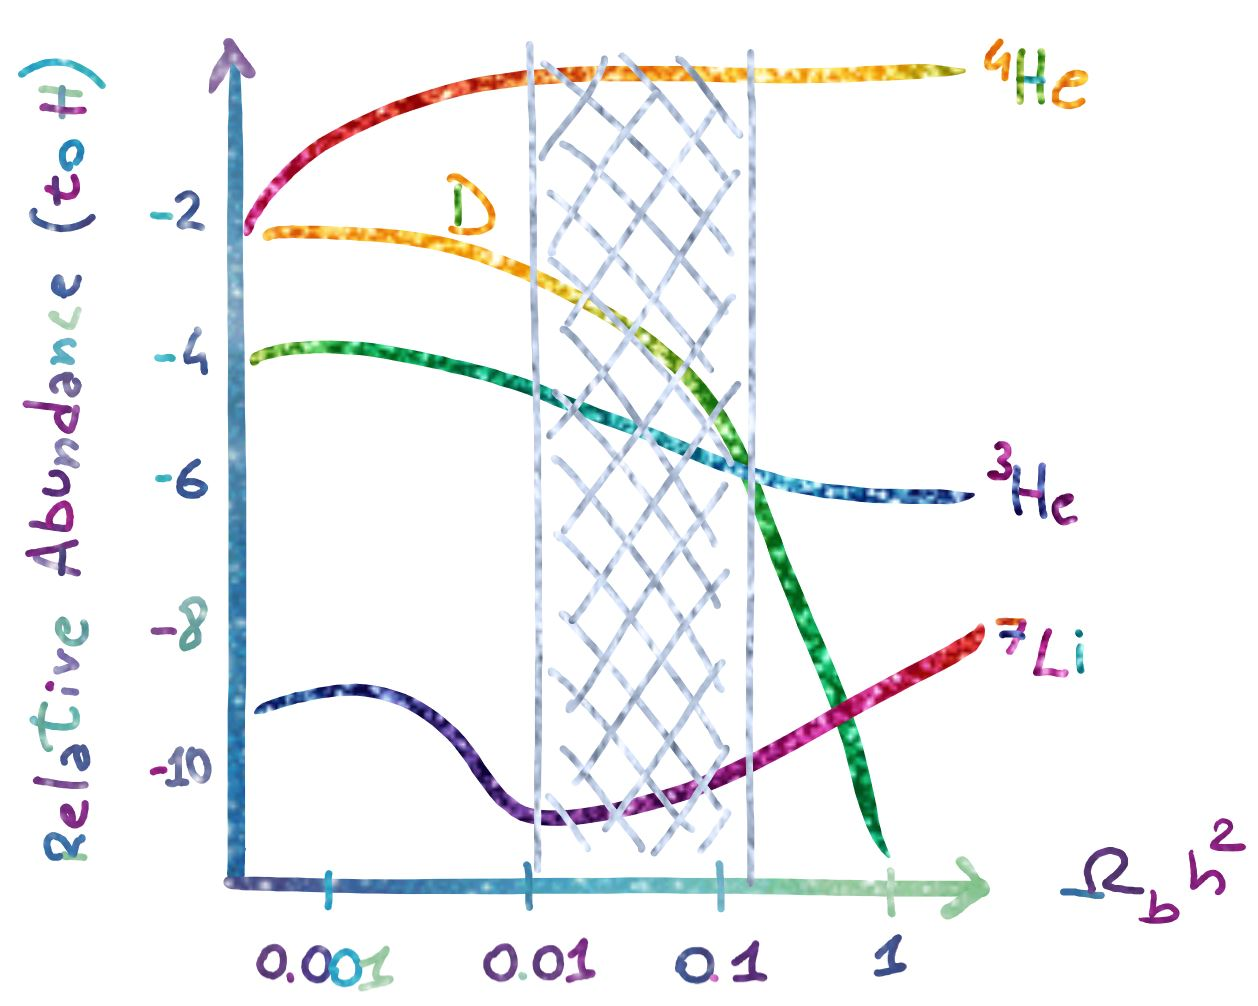
\includegraphics[width=.67\textwidth]{Pictures/5/eleggeriomegab.jpg}
    \caption{Abbondanza relativaall'idrogeno degli elementi leggeri al variare di $\Omegab$. La regione evidenziata corrisponde alle evidenze osservative.}
\end{figure}

\section{Epoca del plasma}
La temperatura diminuisce da $\sim 10^9$ K a $\sim 10^4$ K e l'universo diventa gradualmente più neutro. La successiva re-ionizzazione avverrà solamente per fenomeni di galaxy evolution. Essendo $z_{eq}\sim 1000$, la neutralizzazione formale avviene a $T \sim 2.7\cdot 10^3 $ K.
 In particolare, le principali reazioni e le temperature a cui si ha il 50/50 sono, in ordine:
\begin{equation*}\left\{
    \def\arraystretch{1.5}
        \begin{array}{lll}
        He^{2+}+e^- \leftrightharpoons He^+ + \gamma & 10^4\; \mathrm{K} & \\
        He^+ + e^- \leftrightharpoons He + \gamma &  7\cdot 10^3\; \mathrm{K} & neutralizzazione/\stkout[1pt]{ri}combinazione\; He\\
        H^+ + e^- \leftrightharpoons H + \gamma &  4\cdot 10^3\; \mathrm{K} & neutralizzazione/\stkout[1pt]{ri}combinazione\; H
    \end{array}\right.
\end{equation*}

Prima di questo momento si parla di \textit{epoca del plasma}. 
In una prima fase si hanno: fotoni, $e^-$ e $ p^+$, l'elio (25\% in massa, 6\% in particelle) viene di solito trascurato. Le scale tipiche su cui avvengono le interazioni tra queste componenti sono:

$$ \lambda_D =  \left( \frac{k_BT}{4\pi n_e e^2}\right)^{1/2} \quad \gg \quad \lambda_e \propto n_e^{-1/3} \propto \left ( \frac{m_P}{\rho_{\mathrm{cr},0}\Omegabo}\right)^{1/3} \frac{T_0}{T}$$
Ossia, dentro la sfera di Debye (entro la quale avvengono le interazioni $e^-$ e $p^+$) si ha un gran numero di ioni e quindi un \textit{buon} plasma. Inoltre confrontando il tempo tipico di collisioni tra ioni (attraversamento della sfera di Debye) con il tempo tipico di scattering tra $e^-$ e fotoni (gli $e^-$ perdono momento):
$$ \tau_e = \frac{\lambda_D}{c} \quad \ll \quad \tau_{e\gamma '}=\frac{3m_e}{4\sigma c \rho_r} $$
Per cui non si hanno fenomeni collettivi e $e^-$ e $p^+$ possono considerarsi `accoppiati'. Infine si può verificare che il tempo che serve per mantenerli in equilibrio termico:
$$ \tau_{e^- p^+} = 10^6 (\Omegabo h^2)^{-1} T^{-3/2}\; \textrm{s}  \quad \ll \quad \tau_{exp}$$

Pertanto: elettroni e protoni hanno la stessa temperatura, lo scattering Compton garantisce l'equilibrio con la radiazione e ci si aspetta che questa sia distribuita come un corpo nero.

Le condizioni cambiano quando l'idrogeno \stkout[1pt]{ri}combina.

\subsubsection{Equazioni di Saha}
L'energia di legame dell'idrogeno è $B_H=13.6$ eV corrispondente a una temperatura di $1.6\cdot 10^5$ K. Quando l'universo raggiunge questa temperatura, la temperatura cala ulteriormente rispetto a quanto dettato dal raffreddamento adiabatico. 

Il momento della \stkout[1pt]{ri}combinaizone si fissa quando la frazione di ionizzazione $x=n_e/n_{tot}=0.5$. Elettroni, protoni e idrogeno neutro hanno distribuzione di boltzmann non relativistica (Eq. \ref{eq:boltzmann} sostituendo, per l'$H$, il peso statistico $2$ con $4$). Sapendo che $\mu_p + \mu_e = \mu_H$ e assumendo l'universo elettricamente neutro ($n_e=n_p$):
\begin{equation}
    \frac{n_e n_p}{n_{tot}n_H}=\frac{x^2}{1-x}
\end{equation}
Applicando le distribuzioni di Boltzmann e approssimando $m_p=m_H$:
\begin{equation}
    \frac{x^2}{1-x} = \frac{1}{n_{tot}}\left( \frac{k_B T m_e}{2 \pi \hslash }\right) e^{- B_H / k_B T } 
\end{equation}
Il coefficiente tra parentesi non trascurabile sposta il taglio esponenziale a una temperatura minore di $1.6\cdot 10^5$ K. Inoltre dentro $n_{tot}$ si cela $\Omegabo=0.046^{+0.1}_{-0.01}$, ma in questo caso è la $T$ che comanda. 

\vspace{1em}
La \textbf{ricombinazione} (= prima combinazione) dell'idrogeno avviene quindi a: $$T_{rec,H} \simeq 4000\; \textrm{K} \qquad z_{rec,H}\simeq 1400 \div 1600\quad (1500) $$
Si ricorda che in questo momento si ha 50\% idrogeno neutro e 50\% idrogeno ionizzato, che crollerà esponenzialmente al diminuire di $T$ (stando a questa formula oggi dovrebbe essere $0$, ma non è così per galaxy evolution).
In realtà questa reazione di neutralizzazione non avviene sempre in condizioni di equilibrio (ossia a $\tau_{rec} \sim x/\dt{x} \ll \tau_{exp}$): queste sono già violate a $z\approx 2000$. Svolgendo i conti in condizioni di non equilibrio termico si può verificare che anche a $z\approx few \cdot 100$ c'è una piccola frazione di idrogeno ionizzato, importante per garantire l'accoppiamento materia-radiazione (non spiegabile con solo scattering tra fotoni e idrogeno neutro).

Il vero disaccoppiamento tra le temperature di materia e radiazione è quindi:
$$ z_{dec} \simeq 300 $$

Quando la maggioranza dei fotoni non è più scatterata ed è quindi libera di giungere fino a noi, si osserva la CMB.


La probabilità che un fotone venga scatterato da un elettrone a un certo redshift è:
\begin{equation}
    \mathrm{d}P=-\frac{\mathrm{d}N_\gamma}{N_\gamma}=-\frac{\mathrm{d}I}{I}=\frac{\mathrm{d}t}{\tau_{\gamma e}}=-\d{\tau} \qquad\quad \tau=\int_0^z \frac{xc\rho_m \sigma_T }{m_P}\frac{\d{t}}{\d{z'}}\d{z'}
\end{equation}
Da cui la probabilità che un fotone venga scatterato per l'ultima volta ad un dato redshift è:
\begin{equation}
    -\frac{\d{}}{\d{z}}\left( 1-e^{-\tau} \right)=e^{-\int \tau (z)\d{\tau}}
\end{equation}
Questa probabilità ha una distribuzione gaussiana centrata a $z\simeq 1100$ (detto \textbf{reshift dell'ultimo scattering} con una $FWHM=400$. Questo risultato dipende poco dalla cosmologia. A questi redshift la distribuzione dei fotoni consente di tracciare anche la distribuzione della materia, mentre a redshift maggiori non è possibile ottenere informazioni dalla radiazione.

\newpage
Si hanno quindi tre valori del redshift legati allo stesso fenomeno (ricombinazione dell'idrogeno $z\approx 1000$), ma formalmente diversi:
\begin{example}[Ricombinazione: $\mathbf{z_{rec}=1500}$]
Momento in cui $x=0.5 $
\end{example}
\begin{example}[Disaccoppiamento:  $\mathbf{z_{dec}=300}$]
Momento in cui $T_m=T_r \rightarrow T_m \neq T_r $
\end{example}
\begin{example}[Last Scattering:  $\mathbf{z_{LS}=1100}$]
Picco della distribuzione di probabilità di last scattering.
\end{example}

\vspace{1em}
La conservazione del numero di fotoni $n_\gamma \propto (e^{h\nu /kT}-1)^{-1}$ in un universo in espansione fa sì che la radiazione rimanga distribuita come un corpo nero $I(t_i, \nu)\propto \nu^3 (e^{h\nu /kT}-1)^{-1}$, ma shiftato a frequenze minori, quindi con una $T=T_0(1+z)$. Questo, che è il più bel corpo nero visto in natura è stato osservato dal satellite COBE nel 1991. Una piccola deviazione si verifica a causa dei fotoni generati dalla ricombinazione, ma questo si vede solo nelle code e non nel picco dove $n_\gamma$ è altissimo. Ulteriori deviazioni dal corpo nero possono essere legate a fenomeni di fisica primordiale. In particolare a quelli avvenuti a $10^7 < z < 10^4 $, quando la CMB non sarebbe stata in grado di riportarsi all'equilibrio (a $z$ ancora più alto la termalizzazione è rapidissima, mentre a $z$ ancora più basso il tempo si dilata può termalizzare con calma). Queste vengono dette \textit{anisotropie primarie} e vanno anch'esse cercate nelle code della plankiana. Tra le \textit{anisotropie secondarie} vi è l'effetto Sunyaev–Zeldovich (coming soon...). Con questo si chiude la prima metà del corso, siamo a metà, coraggio!

\chapterimage{/6/head.jpg} % Chapter heading image
\chapter{Un universo... perturbato}\label{6:ch}

\section{Formazione delle Strutture Cosmiche}
La trattazione che segue deriva dalla teoria perturbativa: ossia il campo di densità non si considera perfettamente omogeneo, ma si introducono delle piccole perturbazioni e se ne studia l'evoluzione a partire dalle leggi già studiate. Queste fluttuazioni possono essere originate dall'inflazione. Sono state osservate nel 1991 dal satellite COBE come $\delta T / T \sim 10^{-5}\leftrightarrow \delta \rho / \rho$ (assumendo adiabaticità) a $z=1100$ e come $\delta \rho /\rho \sim 10^{2\div 3}$ attraverso la struttura a grande scala a $z=0$.

Esiste una scala fisica (detta \textit{di Jeans}) oltre la quale si ha il collasso gravitazionale e si ottiene ponendo:

\begin{example}[$\mathbf{E_{kin}=E_{pot}}$]
    $R_J \propto v \sqrt{\frac{1}{2 G \rho}} $
\end{example}
\begin{example}[$\mathbf{\bar{F}_{press}=\bar{g}}$]
    $R_J \propto v_s \sqrt{\frac{1}{G \rho}} $
\end{example}
\begin{example}[$\mathbf{\tau_{free\, fall}=\tau_{sound\, crossing}}$]
        $R_J \propto v_s \sqrt{\frac{1}{2 G \rho}} $
\end{example}
In ambetrè i casi ci sono due processi in competizione: da una parte la gravità, dall'altra la dispersione di velocità / pressione / attraversamento. 
Per scale $R>R_J$ si ha collasso gravitazionale, per quelle più piccole la perturbazione si dissolverà.

%\begin{theorem}[Principio dell'instabilità gravitazionale]
%Piccole perturbazioni crescono.
%\end{theorem}

\section{Teoria di Jeans Classica}
Il metodo utilizzato consiste nell'applicare piccole perturbazioni ad uno stato di equilibrio stazionario, omogeneo e isotropo. Soluzioni analitiche si possono trovare solamente in regime lineare e verranno espresse sotto forma di serie di Fourier. Le equazioni fondamentali sono: conservazione della massa, del momento (Eulero) ed equazione di Poisson, a queste si aggiunge un'equazione di stato:
\begin{equation}\left\{
    \def\arraystretch{1.5}
        \begin{array}{l}
        \rho_t + \nabla \rho \cdot \vec{v} + \rho \nabla \cdot \vec{v} =0\\
        \rho \left (  \vec{v}_t + (\vec{v}\cdot \nabla )\vec{v}\right)=-\nabla p + \rho \nabla \phi \\
        \nabla^2 \phi = -4\pi G \rho \\
        p=p(\rho, S) 
    \end{array}\right. \label{eq:6planksys}
\end{equation}
ove il pedice indica la derivazione parziale rispetto al tempo. 

Si considereranno, così come corroborato dalle osservazioni, solamente soluzioni adiabatiche: $p(\rho, S)\rightarrow p(\rho)$. Lo stato di equilibrio si introduce ipotizzando che le costanti $\rho_0$, $p_0$, $\phi_0$ (``di background'') soddisfino il sistema (\ref{eq:6planksys}). In realtà questa soluzione non è ammissibile fisicamente poiché $\phi_0 = cost \Leftrightarrow \rho_0=0 $, ma è comunque didattica. Lo stesso non si verificherà quando saranno considerate le soluzioni di Friedmann $\rho_0(t)$, $\phi_0(t)$, $v_{exp}$.

Il sistema linearizzato che governa le piccole perturbazioni, sapendo che $c_s^2 = \left . \frac{\partial p}{\partial \rho} \right |_{S=cost}$, è:
\begin{equation}\left\{
    \def\arraystretch{1.5}
        \begin{array}{l}
        \delta\rho_t + \rho_0\nabla\cdot \delta \vec{v} =0 \\
        \rho_0 \left ( \delta \vec{v}_t + c_s^2 \nabla \delta_k - \nabla \delta\phi \right) = 0 \\
        \nabla^2 \delta \phi = -4\pi G \delta\rho
    \end{array}\right. 
\end{equation}
ove $\delta_k=\delta \rho / \rho_0$ e per $\delta \rho_k$ si intende $(\delta\rho)_k$. Si nota che i termini dipendenti solamente dalle quantità di backgruond si semplificano poiché soddisfano le equazioni del sistema (\ref{eq:6planksys}).

Si cercano soluzioni/perturbazioni separate nella dipendenza spazio-tempo nello spazio di Fourier: $S(\vec{r},t)=S_k \: e^{i(\vec{k}\cdot\vec{r}-\omega t)}$. Per cui valgono le relazioni: $S_t = -i\omega S$, $\nabla S = i\vec{k}S$ e $\nabla^2 S= -k^2 S$ e nella direzione longitudinale al moto ($\vec{k}\cdot\vec{v}=kv$) si ottiene il seguente sistema di dispersione:
\begin{equation}\left\{
    \def\arraystretch{1.5}
        \begin{array}{l}
        - \omega \delta_k + k \delta v_k = 0 \\
        - \omega \delta v_k + k (c_s^2\delta_k -\delta\phi_k) = 0 \\
        - k^2 \delta\phi_k = -4\pi G\delta\rho_k
    \end{array}\right. 
\end{equation}
che definisce la relazione tra l'ampiezza dell'onda del contrasto di densità con l'ampiezza dell'onda del contrasto di velocità. Questo è reso più evidente dall'\textbf{equazione di dispersione} che si ottiene annullando determinante del sistema:
\begin{equation}
    \omega^2 = c_s^2 k^2 - 4\pi G \rho_0 \label{eq:6disprelstatic}
\end{equation}
Per $\omega^2 < 0 \rightarrow \omega \in \mathbb{C}$ si hanno due soluzioni esponenziali: una crescente e una decrescente. Per $\omega^2 > 0 \rightarrow \omega \in \mathbb{R}$ si hanno due onde di piccola ampiezza logitudinali con verso opposto. Con la condizione $\omega^2 = 0$ vengono definiti il \textit{numero d'onda di Jeans} (che verrà spesso chiamato impropriamente \textit{scala di Jeans}) e la \textit{lunghezza d'onda di Jeans} ($k=2\pi /\lambda$):
\begin{equation}
k_J = \sqrt{\frac{4\pi G \rho_0}{c_s^2}} \qquad \lambda_J=c_s\sqrt{\frac{\pi}{G\rho_0}} \qquad \omega^2=k^2 c_s^2 \left[1- \left(\frac{\lambda}{\lambda_J}\right)^2\right]
\end{equation}

Quindi ricapitolando si ha:
\begin{itemize}
    \item $\lambda >\lambda_J$ oppure $k<k_J$: $\delta = \delta_k e^{\mp |\omega| t}e^{ikr} $ onda con stessa forma spaziale, ma ampiezza che dampa o esplode. Quest'ultimo caso (crescente) è quello interessante da un punto di vista cosmologico.
    \item $\lambda <\lambda_J$ oppure $k>k_J$: la perturbazione rimane sotto forma di due onde, una receding e una proceding, di ampiezza costante.
    \item $\omega^2=0$ è come se l'onda si congelasse ($v_{fase}=0$)
\end{itemize}

\vspace{1em}
\noindent Questa trattazione vale fintantoché $\delta \ll 1$ (osservativamente i galaxy clusters arrivano anche a $1000$). Inoltre, includendo l'effetto dell'espansione dell'universo ci si aspetta una crescita delle perturbazioni più lenta di quella esponenziale.



\section{Teoria di Jeans Cosmologica}
Per la trattazione cosmologica è necessario considerare tre scale fondamentali:
\begin{enumerate}
    \item $R_H$ discrimina le scale sotto cui va considerata la microfisica, per $R>R_H$ l'unica interazione fondamentale da considerare è la gravità;
    \item $R_J$ sarà rilevante solo se $<R_H$;
    \item $R_d$ ossia la scala di dissipazione delle onde (differente per la materia ordinaria e quella oscura).
\end{enumerate}
Le prime due sono evidentemente variabili nel tempo.

Entrano poi in gioco due tempi fondamentali:
\begin{enumerate}
    \item $t_{equivalence}$ discrimina la dominanza di radiazione/materia;
    \item $t_{decoupling}$ la pressione di radiazione impedisce il collasso della materia se accoppiata, inoltre come si è visto $t_{dec,DM} < t_{eq} < t_{rec,b}$.
\end{enumerate}

Si utilizzano le equazioni di Friedmann considerando la perturbazione come un piccolo universo chiuso immerso in un universo di background meno denso e piatto (per semplificare i conti). La soluzione è relativistica, ma in questo caso si sta considerando solamente la gravità, per cui sarà valida per: scale maggiori di $R_H$ o minori di $R_H$, ma sufficiendemente più grandi della $R_J$. 

Tramite la seconda equazione di Friedmann si ha rispettivamente per perturbazione e background:
\begin{equation}\left\{
    \def\arraystretch{1.5}
        \begin{array}{l}
            H_p^2=\frac{8\pi }{3}G \rho_p - \frac{c^2}{a^2}\\
            H_b^2 =\frac{8\pi}{3}G \rho_b
    \end{array}\right. \quad\leftrightarrow\quad \delta = \frac{3c^3}{8\pi G \rho_b a^2}\propto \left(\rho_b a^2\right)^{-1}\propto a^{1+3w}\propto
    \left\{
   \begin{array}{ll}
        a^2 & t<t_{eq}\\
        a & t>t_{eq}
\end{array}\right. 
\end{equation}
dove si sono sincronizzati gli universi ponendo $H_p=H_b$.

\subsection{Soluzione per $\mathbf{R > R_H}$}
Fuori dall'orizzonte solo la gravità domina le cose, le altre componenti seguono la gravità, pertanto:
\begin{equation}
    \def\arraystretch{1.5}
        \begin{array}{ll}
        \delta_m \bowtie  \delta_R \propto a^2 & t<t_{eq} \\
        \delta_R \bowtie  \delta_m \propto a & t>t_{eq} 
    \end{array} \label{eq:unitaplanckiane}
\end{equation}
Le perturbazioni crescono tutte in modo uguale e le componenti sottodominanti seguono quella dominante.

\begin{theorem}[Messaggio da portare a casa]
Fuori dall'orizzonte le perturbazioni crescono sempre, ma con un andamento che cambia a $t_{eq}$. Prima seguono l'andamento della radiazione, dopo quello della materia. Attenzione però: $R_H=R_H(t)$.
\end{theorem}


\subsection{Soluzione per $\mathbf{R < R_H}$}\label{ch6:chilovoleva}
Per trovare le soluzioni all'interno dell'orizzonte bisogna tener conto dell'espansione dell'universo. Le coordinate che contano sono quelle fisiche ($r$) , ma passando alle coordinate comoventi ($x$) si possono semplificare i conti: $r=a/a_0 \; x$, di solito $a_0=1$. Si può dimostrare che $\d{r}/\d{t} = Hr + a\dot{x} = Hr+ v_{pec}$. La $v_{pec}$ sarà la perturbazione rispetto al flusso di Hubble, dovuta alla disomogeneità della materia. Utilizzando $u=\dot{r}$, si può riscrivere il sistema per il modello fisico:
\begin{equation}\left\{
    \def\arraystretch{1.5}
    \begin{array}{l}
        \rho_t + \nabla\cdot (\rho \vec{u}) =0 \\
        \rho \left ( \vec{u}_t + (\vec{u} \cdot \nabla) \vec{u} \right) = -\nabla p +\rho \nabla \phi \\
        \nabla^2 \phi = - 4 \pi G \rho
    \end{array}\right.
\end{equation}
In questo caso si cercano soluzioni del tipo: $\rho = \rho_0 (1+\delta)$, $u=Hr+v_{pec}$, $\phi=\phi_0+\delta\phi$ e $p=p_0+\delta p$. Il sistema linearizzato che governa le piccole perturbazioni diventa:
\begin{equation}\left\{
    \def\arraystretch{1.5}
    \begin{array}{l}
        \delta\rho_t + \rho_0 \nabla\cdot\vec{v}_{pec} + 3H \delta\rho + Hr \nabla \delta\rho \cdot \hat{r} =0 \\
        \rho_0 \left ( \vec{v}_{pec, t} + H \vec{v}_{pec}+ Hr\nabla\vec{v}_{pec}\right ) = -c_s^2 \nabla\delta\rho +\rho_0\nabla\phi \\
        \nabla^2 \delta \phi = -4\pi G \delta\rho
    \end{array}\right.
\end{equation}
A questo punto si cambia il sistema di riferimento in coordinate comoventi per ``riassorbire'' l'espansione dell'universo (le coordinate comoventi non dipendono dal tempo). In particolare gli operatori diventano:
\begin{equation*}
    \def\arraystretch{1.5}
    \begin{array}{l}
        \nabla_r = \frac{1}{a}\nabla_x \\
        \frac{\d{f}}{\d{t}} = \left. \frac{\partial}{\partial t} \right|_r f + Hr \nabla_r f = \left. \frac{\partial}{\partial t} \right|_x f + 0 \qquad \rightarrow \qquad \left. \frac{\partial}{\partial t} \right|_r f = \left. \frac{\partial}{\partial t} \right|_x f - Hr \nabla_r f  
    \end{array}
\end{equation*}
Quindi il sistema in coordinate comoventi diventa:
\begin{equation}\left\{
    \def\arraystretch{1.5}
    \begin{array}{l}
        \delta\rho_t + \frac{\rho_0}{a} \nabla \cdot\vec{v}_{pec} + 3H \delta\rho =0 \\
        \rho_0 \left ( \vec{v}_{pec, t} + H \vec{v}_{pec} \right) = -\frac{c_s^2}{a} \nabla\delta\rho +\frac{\rho_0}{a}\nabla\phi \\
        \frac{1}{a^2}\nabla^2 \delta \phi = -4\pi G \delta\rho 
    \end{array}\right.
\end{equation}
Si  cercano  soluzioni/perturbazioni  nello  spazio  di Fourier nella forma: $S(r,t) =S_k (t)\: e^{ikx}$, poiché già si sa che le ampiezze dipenderanno dal tempo. Includendo l'evoluzione  si ottiene il seguente sistema di dispersione: 

\textbf{Dopo l'equivalenza} il background è dominato dalla materia, per cui: $\rho_0 \propto a^{-3}$, $p_{rad}=0$.
\begin{equation}\left\{
    \def\arraystretch{1.5}
    \begin{array}{l}
        \dot{\delta}_{k} + \frac{i\vec{k}\cdot\vec{v}_k}{a}=0 \\
        \dot{\vec{v}}_k + H \vec{v}_k = -\frac{i\vec{k}}{a}\left( v_s^2 \delta_k + \delta\phi_k\right) \\
        \delta\phi_k = \frac{4 \pi G \delta \rho_k a^2}{k^2}
    \end{array}\right.
\end{equation}
dove per alleggerire la notazione si è utilizzato il punto per le derivate temporali e $v=v_{pec}$. A questo punto si scompone il campo di velocità lungo la terna ortonormale del vettore d'onda \{$\hat{n}$, $\hat{t}_1$, $\hat{t}_2$\} dove la prima componente rappresenta la direzione longitudinale / parallela a $\vec{k}$ e le altre due formano il piano perpendicolare ad essa. In questo modo si ha:
$$
\vec{v}_k = \vec{v}_{k,\perp} + \vec{v}_{k,\parallel} \qquad \rightarrow \qquad \nabla \cdot \vec{v}_{k,\perp} = 0; \quad \nabla \times  \vec{v}_{k,\parallel} =0
$$
L'equazione di Eulero per la componente perpendicolare si riduce a $\d{( a\vec{v}_{k,\perp})}/\d{t}=0 \rightarrow \vec{v}_{k,\perp}\propto a^{-1}$. Questo significa che, se l'universo si espande, l'eventuale componente rotazionale del campo di velocità decresce nel tempo e si può quindi trascurare.
Aggiornando il sistema per la componente longitudinale e svolgendo le dovute operazioni cosmatematiche (tra cui riportare le coordinate al sistema fisico $k/a\rightarrow k$) si ottiene l'\textbf{equazione di dispersione} per il modello in esame:
\begin{equation}
    \ddot{\delta}_k + 2 \frac{\dot{a}}{a}\dot{\delta}_k + \delta_k \left( k^2 c_s^2 -4\pi G \rho_0\right) =0 \label{eq:6disprelmat}
\end{equation}
La quale per un universo statico (derivate temporali nulle) si riconduce all'equazione \ref{eq:6disprelstatic}.

La cosmologia è nascosta in $\dot{a}/a$ e in $\rho_0$ nella relazione tra redshift e tempo.


\subsubsection{Universo EdS di sola materia}
Applicando le relazioni ricavate nel paragrafo \ref{6:chsub:eds} si cercano soluzioni nella forma $\delta_k \propto t^\alpha$:
\begin{equation*}
3\alpha^2 + \alpha + 2\left( \frac{k^2 c_s^2}{4\pi G \rho_0}-1\right)=0
\end{equation*}
Il valore che annulla il discriminante è $k_J= \sqrt{25\pi G \rho_0 /6c_s^2}$. Si hanno due soluzioni reali ($\Delta >0$, $k<k_J$, $\lambda >\lambda_J$) se:
\begin{equation*}
\alpha_{1,2}=-\frac{1\pm 5\sqrt{1-\left( \lambda_J /\lambda\right)^2}}{6}
\end{equation*}
La soluzione interessante è quella crescente, che dipende da quanto la lunghezza d'onda delle perturbazioni è vicino a quella di Jeans.
Per $\lambda \gg \lambda_J$ (si può trascurare il termine con $c_s$ rispetto a quello gravitazionale) si ha:
\begin{equation}\delta_k \propto  \left\{
    \def\arraystretch{1.5}
        \begin{array}{ll}
            t^{-1} & trascurabile \\
            t^{2/3} \propto a & 
    \end{array}\right. 
\end{equation}
Ossia le perturbazioni negli universi EdS in regime lineare per scale molto più grandi di quella di Jeans crescono come il fattore di espansione. Per scale più vicine a $\lambda_J$ ci si aspetta un rallentamento dovuto agli effetti di interazione del fluido fino ad arrivare ad uno stato stazionario. Si ricorda che tutto questo vale dopo il disaccoppiamento dalla radiazione, momento che avviene prima per la materia oscura rispetto a quella barionica.

\subsubsection{Universo Curvo di sola materia}
Svolgendo la derivata seconda di $H=\dot{a} / a$, inserendo la seconda equazione di Friedmann per la materia e derivando ulteriormente si ha:
\begin{equation*}
    \ddot{H}+2H\dot{H}-4\pi G \rho_0 H = 0 \qquad vs. \qquad (6.12) \quad \ddot{\delta}_k + 2 \frac{\dot{a}}{a}\dot{\delta}_k + \left( k^2 c_s^2 -4\pi G \rho_0\right) \delta_k  =0
\end{equation*}
Per $\lambda \gg \lambda_J$ il termine con $c_s^2$ è trascurabile, pertanto ci si aspetta che le soluzioni siano le stesse ottenute in precedenza con $\delta_k \rightarrow H$. Quando si sono cercate le soluzioni all'equazione di Friedmann è stata imposta l'espansione dell'universo ($H_0 > 0$), sciegliendo formalmente una delle due possibili soluzioni. Questa, mediante l'analogia, corrisponderebbe alla soluzione decrescente, $\delta_-$, ossia quella meno intrigante. Ancor meno intrigante è il teorema del Wronskiano $W$, che ci consente, avendo due signore funzioni (derivabili, ecc..) di ottenere la soluzione crescente:
$$
y''+Py'+Qy=0 \qquad W=y_1'y_2 - y_1y_2'; \; W'=-PW \quad \rightarrow \quad W=\delta_-\dot{\delta}_+ - \dot{\delta}_-\delta_+ \propto a^{-2}
$$
Integrando il differenziale del rapporto tra $\delta_+$ e $\delta_-$ si ottiene la relazione tra le due soluzioni:
\begin{equation*}
    \delta_+ = \delta_- \int \frac{\delta_-\dot{\delta}_+ - \dot{\delta}_-\delta_+}{\delta_-^2}\d{t}\quad\propto\quad \delta_- \int \frac{\d{t}}{\delta_-^2\: a^2}
\end{equation*}
Essendo $\d{z}=-H(1+z)\d{t}$ si ottiene l'evoluzione del cosiddetto \textbf{growing factor}:
\begin{equation}
    \delta_+ = -\frac{H(z)}{a_0^2}\int \frac{1+z}{H^3}\d{z}
\end{equation}
In generale questo integrale non ha soluzione analitica (si ricorda che $H=H_0 E$). Nei modelli EdS la crescita va come $a\propto (1+z)^{-1}$, ci si aspetta una crescita inferiore negli universi aperti e una crescita superiore in quelli chiusi (nei quali diminuisce il termine di ``frizione'' dovuto all'espansione).

\begin{figure}[H]
    \centering
    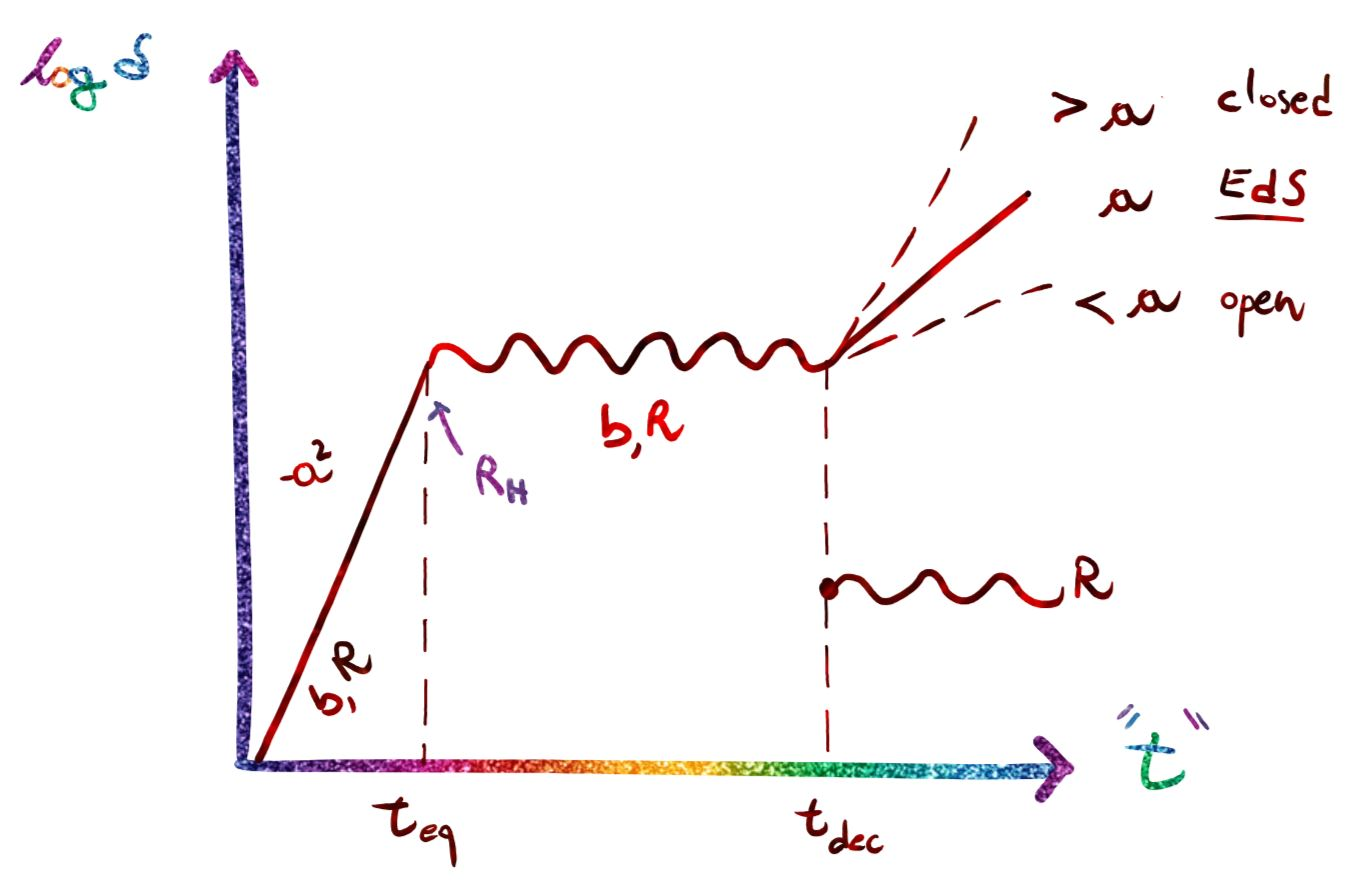
\includegraphics[width=.55 \textwidth]{Pictures/6/growingfactor.jpg}
    \caption{fig:4 occhio che delta deve essere minore di 1. Occhio che rinormalizzando le curva ad oggi chiuso e aperto si scambiano sopra-sotto}
\end{figure}

In realtà esiste una relazione analitica che fa uso di $f=\d{\log \delta_+} / \d{\log a}$ per riscalare la crescita:
\begin{equation*}
    f=\Omega_m^{0.55} - \frac{\Omega_\lambda}{70} (1+\Omega_m /2)
\end{equation*}
All'aumentare della materia le perturbazioni crescono più velocemente, mentre la costante cosmologica è meno influente. Per $\Omega_m=1$ si recuera l'andamento $\delta_+ \propto a$. Il numero $0.55$ è magico poiché è una delle predizioni precise della relatività generale. Osservando la variazione del fattore di crescita al variare di $\Omega_m$ si può falsificare la teoria della relatività generale. Altrimenti si possono porre constraints sulla cosmolgia (conteggio ammassi al variare di z, tomografia weak lensing).

\vspace{1em}
Fluttuazioni nella desità sono state osservate come $\delta T /T \sim 10^{-5}$ nella CMB ($z\sim 10^3$). Utilizzando le relazioni trovate in regime lineare, ci si aspetterebbe: $\delta (z=0) \sim 10^{-2}$ contrariamente a quanto osservato $\delta_{obs} (z=0)\sim 100$ (regime chiaramente non linerare). Ragionando in modo opposto, si fissa $\delta (z=0) = 1 $ (ipotizzando che sia diventato $\sim 100$ ieri l'altro), questo richiede che $\delta_{CMB}\sim 10^{-3}$. Un modo per giustificare il fatto che non si osserva è ricorrere agli universi chiusi, ma servirebbe $\Omega \approx 10$ (alèèè, un pò troppo chiuso!). La soluzione è ipotizzare che i barioni crescono come $a$ e che attorno a loro vi è una distribuzione di DM non più uniforme (avviene come si vedrà il \textit{barion ``ketchup''}). Questa può anche essere vista come una delle prove a favore dell'esistenza della DM, che aiuta a far crescere le perturbazioni essendosi disaccoppiata prima.
\vspace{1em}


\subsubsection{Universo EdS di sola radiazione}
\textbf{Prima dell'equivalenza} non si può trascurare il contributo della pressione di radiazione, per cui nelle equazioni del sistema \ref{eq:6planksys} va fatta la sostituzione $\rho \rightarrow \rho + 3p/c^2$ ($c_s=c/\sqrt{3}$). Analogamente a come si è fatto in precedenza: si ipotizza che esista una soluzione imperturbata data dall'espansione dell'universo, si aggiunge una piccola perturbazione e si linearizzano le equazioni. Si ottiene la seguente \textbf{equazione di dispersione}:
\begin{equation}
    \ddot{\delta}_k + 2 \frac{\dot{a}}{a}\dot{\delta}_k + \delta_k \left( k^2 c_s^2 -\frac{32}{3}\pi G \rho_0\right) =0
\end{equation}
Applicando le relazioni per un universo EdS di sola radiazione (Paragrafo \ref{6:chsub:eds}, $w=1/3$) si cercano soluzioni sotto forma di $\delta_k \propto t^{\alpha -1}$:
\begin{equation*}
    \alpha^2 = 1-\frac{3k^2c_s^2}{32 \pi G\rho_0}
\end{equation*}
Pertanto di definisce: $k_J=\sqrt{32\pi G \rho_0 / 3c_s^2}$. Si hanno due soluzioni reali ($\alpha^2=0$, $k<k_J$, $\lambda >\lambda_J$) se:
\begin{equation*}
    \alpha_{1,2}=\pm \sqrt{1-\left( \lambda_J /\lambda\right)^2}\qquad \rightarrow \qquad \alpha_{1,2}=\pm 1 \quad per\; \lambda \gg \lambda_J
\end{equation*}
La dipendenza interessante è quindi $\delta_k \propto t^1$ a differenza dell'andamento $t^{2/3}$ per la materia, ossia dopo l'equivalenza. Il problema sta nel capire quanto è grande la scala di Jeans rispetto alla scala dell'orizzonte. La relazione di dispersione può essere riscritta nella forma: $1-k_J^2c_s^2t^2 = 0$, ossia ($c_s=c/\sqrt{3}$): 
\begin{equation*}
    k_J = \sqrt{3}/ct \qquad\rightarrow \qquad \lambda_J = 2\pi c t /\sqrt{3} \quad > \quad R_H = 2ct
\end{equation*}
La scala di Jeans è quindi più grande della scala dell'orizzonte: il problema sta nel fatto che la scala di Jeans non sta dentro l'orizzonte e non ha quindi senso fisico (fuori dall'orizzonte le perturbazioni crescono sempre, non hanno una scala). Questo significa che \textbf{non c'è la possibilità di far crescere le perturbazioni durante l'era radiativa}. Inoltre, il fatto che le perturbazioni si stiano propagando così velocemente, fa si che mediamente $\delta_R =0$ e di conseguenza tutte le altre componenti accoppiate. Tradotto in altro modo, la pressione di radiazione è talmente forte che impedisce il collasso.

\vspace{1em}
Per la \textbf{materia oscura} vale l'equazione di dispersione \ref{eq:6disprelmat}, che deve essere riadattata per l'epoca radiativa e per la materia oscura. In particolare $c_s^2$ diventa la pressione/dispersione di velocità della DM e nel termine gravitazionale bisogna considerare tutte le componenti: $\rho_0 \delta_k \rightarrow \rho_R\delta_R + \rho_{bar}\delta_{bar} + \rho_{DM}\delta_{DM} $. La prima è trascurabile poiché, come appena visto, non ci sono contrasti nella componente relativistica e pure la componente barionica poiché è ad essa accoppiata. L'\textbf{equazione di dispersione} diventa:
\begin{equation}
    \ddot{\delta}_{k,DM}+ 2 \frac{\dot{a}}{a}\dot{\delta}_{k,DM} + \left( k^2 c_s^2 -4\pi G \rho_{0,DM}\right)\delta_{k,DM}  =0
\end{equation}
Ancora una volta si cercano soluzoni per $\lambda \gg \lambda_J$. È conveniente cambiare variabile utilizzando $x=a/a_{eq}\rightarrow \frac{\d{}}{\d{t}}=\frac{\dot{a}}{a_{eq}}\frac{d{}}{\d{x}}\rightarrow \frac{\d{}^2}{\d{t^2}}=\frac{\ddot{a}}{a_{eq}}+\frac{\d{}}{\d{x}}+\left(\frac{\dot{a}}{a_{eq}}\right)^2 + \frac{\d{}^2}{\d{x^2}}$. In seguito si inserisce l'evoluzione delle densità in funzione di $a$, in particolare: $\rho_{DM} (a) / \rho_R(a) = x$. Per eliminare le dipendenze da $\dot{a}$ e $\ddot{a}$ si utilizzano infine le rispettive equazioni di Friedmann, dove la densità è data da $\rho_{DM}+\rho_{R}$ e la pressione $p_{DM}+p_R$:
\begin{equation*}
    \rho_{DM}=\frac{3H^2 x}{8\pi G (1+x)}; \qquad \frac{\dot{a}}{a_{eq}}=Hx; \qquad \frac{\ddot{a}}{a_{eq}}=-\frac{x(x+2)H^2}{2(x+1)};   
\end{equation*}
Con un po' di \textit{maquillage} si ottiene:
\begin{equation}
    \delta_{k,DM}'' + \frac{3x+2}{2x(1+x)}\delta_{k,DM}' - \frac{3}{2x(1+x)}\delta_{k,DM}=0
\end{equation}
Dove l'apice indica la derivata rispetto a $x$. Questa è un'equazione ipergeometrica che ha come soluzione crescente: $\delta_{k,DM}^+ = 1+3x/2$ valevole entro l'orizzonte  solo prima dell'equivalenza, inoltre:
\begin{equation}
    \frac{\delta (t_{eq})}{\delta(t_H)}=\frac{1+3/2}{1+3a_H/2a_{eq}} \quad < \quad 5/2
\end{equation}
Questo rappresenta il fattore di crescita delle perturbazioni di materia oscura dal momento in cui queste entrano nell'orizzonte fino al momento per cui la soluzione è valida (il tempo dell'equivalenza). L'entrata nell'orizzonte può avvenire al più quando $a_H\rightarrow 0$ (un istante dopo il BB). Dopo l'equivalenza la crescita riprende con le leggi già viste. 

\begin{definition} 
Le perturbazioni di DM dentro l'orizzonte possono crescere fino a $t_{eq}$ al più di un fattore $5/2$ (una cavolatina). Questo viene detto \textbf{effetto di stagnazione} o \textbf{effetto Meszaros}. In altri termini, nell'epoca dominata dalla radiazione il tempo scala di espansione dell'universo è minore del tempo scala di collasso delle perturbazioni di DM (il campo dominante, quello radiativo, non ha fluttuazioni).
\end{definition}

La teoria lineare lontano dalla $\lambda_J$ non prevedeva una dipendenza dalla scala, che viene invece introdotta dall'effetto Meszaros. Le scale che sono potute entrare nell'orizzonte prima dell'equivalenza sono infatti modificate. 


\begin{figure}[H]
    \centering
    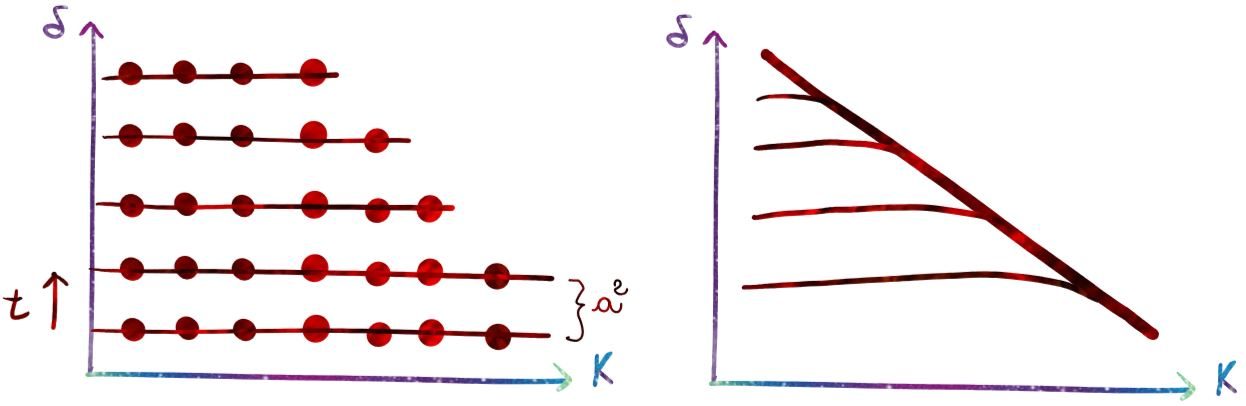
\includegraphics[width=.95 \textwidth]{Pictures/6/meszarus.jpg}
    \caption{Sinistra: Si suppone che inizialmente le perturbazioni nascono tutte uguali, indipendente da $k$ (in realtà non sarà così). Ogni punto rappresenta discretamente una perturbazione sulla scala $k$. Fuori dall'orizzonte le perturbazioni crescono come $a^2$ indipendentemente dalla scala. La prima scala ad entrare nell'orizzonte è quella con $\lambda$ più piccolo, ossia con $k$ più grande. I punti che entrano nell'orizzonte stagnano, pertanto l'altezza delle perturbazioni non è più costante e viene introdotta una dipendenza da $k$. Dopo l'equivalenza, la crescita torna ad essere indipemndente da $k$, quindi si formeranno curve autosimilari. L'evoluzione cumulativa è mostrata nella figura a destra.}
\end{figure}


\subsection{Fluttuazioni barioniche}
I poveri barioni hanno la sfortuna/fortuna di essere accoppiati alla radiazione fino a $z\sim 1000$.  Vorrebbero fare gravità e collassare, ma la pressione di radiazione lo impedisce ed essi oscillano. In seguito alla ricombinazione dell'idrogeno il barione si accorge di esser tale, ma nel frattempo la materia oscura, disaccoppiandosi prima, ha potuto fare i suoi porci comodi. Per questo motivo i barioni si trovano le buche di potenziale della materia oscura già belle che formate. Inizialmente, il contrasto di densità dei barioni risponde a un capo gravitazionale prodotto dalla DM e l'\textbf{equazione di dispersione} è:
\begin{equation}
    \ddot{\delta}_{k,b}+ 2 \frac{\dot{a}}{a}\dot{\delta}_{k,b} + \left( k^2 c_s^2 -4\pi G \rho_{0,DM}\right)\delta_{k,DM}  =0
\end{equation}
Assumendo un universo EdS $\delta_{k,DM}=Aa$, indicando con l'apice la derivata rispetto ad $a$ e utilizzando le equazioni di Friedmann come nel conto precedente (qui $\rho_{DM}\gg\rho_{b}$):
\begin{equation*}
    \frac{2}{3}a\delta_{k,b}''+\delta_{k,b}' -A=0
\end{equation*}
Si cerca una soluzione crescente del tipo $\delta_{k,b}=Ba+C$ e si trova che l'equazione è soddisfatta se $B=A$. Ponendo la condizione iniziale $\delta_{k,b}(t_{dec})=0$ (poiché i barioni non hanno avuto la possibilità di fare disomogeneità prima dell'equivalenza), si ha: $C=-Aa_{dec}$. La soluzione, valida per $a>a_{dec}$, diventa:
$$
\delta_{k,b}=\delta_{k,DM}\left(1-\frac{a_{dec}}{a}\right)
$$
La crescita dei barioni è legata a quella della DM, parte da 0 e col passare del tempo raggiunge asintoticamente la $\delta_{k,DM}$. Questo viene chiamato \textbf{baryon catch-up}. Oggi ci si aspetta che i contrasti di densità siano uguali entro una parte su 1000. 

\vspace{1em}
\noindent Si stanno assumendo perturbazioni adiabatiche (l'entropia si conserva) per cui da $S\propto T^3/\rho_m$ si ha:
$$
0=\frac{\d{S}}{S}=3 \frac{\d{T}}{T}=-\frac{\d{\rho_m}}{\rho_m}
$$
Quindi ci si aspetta che le fluttuazioni del campo di densità della materia siano proporzionali alle fluttuazioni del campo di temperatura. 

\vspace{1em}
\begin{example}[Universo di barioni e radiazione] Si studia il comportamento di quello specifico $\delta$ che entra nell'orizzonte al momento dell'equivalenza. Inizialmente $\delta_b \bowtie \delta_R$ e crescono come $a^2$, all'interno dell'orizzonte oscillano fino al disaccoppiamento, momento dopo il quale $\delta_b$ cresce come materia normale e la radiazione decade non avendo più il supporto dei barioni. Già negli anni `70-`80 gli strumenti sarebbero stati in grado di misurare fluttuazioni dell'ordine di $\delta_{dec}\sim 10^-4$, ma non si sono osservate. In particolare, come già calcolato, per un universo EdS si sarebbe dovuto misurare $\delta_{dec}\sim 10^{-3}$. Potrebbe allora essere chiuso? Si, ma la signora nucleosintesi afferma che i barioni non possono essere più del 15-20\% in $\Omega$... quindi no.
\end{example}

\vspace*{-2em}
\begin{figure}[H]
    \centering
    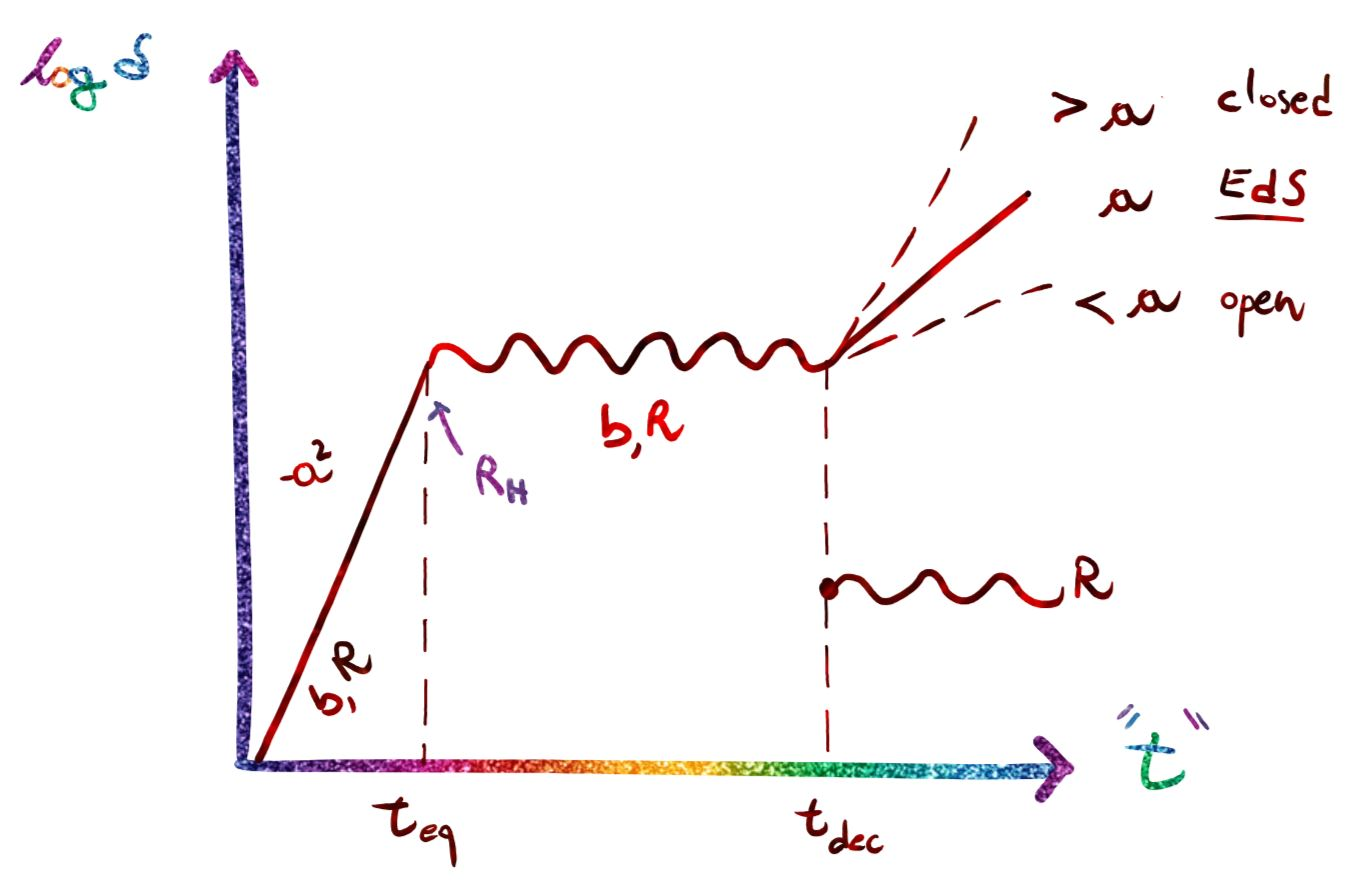
\includegraphics[width=.9 \textwidth]{Pictures/6/growingfactor.jpg}
    \caption{non fidarsi delle concavità}
\end{figure}


\vspace*{-2em}
\begin{example}[Universo di materia oscura, barioni e radiazione]
Per radiazione e barioni si ripete lo scenario appena visto con $\delta_b,\; \delta_{DM} \bowtie \delta_R$. La materia oscura, dopo l'equivalenza, continua però a crescere come $a$ (è lecitissimo assumere EdS in questo periodo). Questo perché la materia oscura si è già disaccoppiata. Questo fenomeno genera una differenza di altezza fra il contrasto di densità della DM e quello dei barioni, che verrà recuperata a partire da $t_{dec}$ (baryon catch-up). Gli ordini di grandezza di $\delta$ in più (fino 3 dex) rispetto a prima sono un regalo della DM.
[Considerando perturbazioni che entrano nell'orizzonte prima dell'equivalenza, si avrebbero plot leggermente diversi (effetto della stagnazione, ecc...)]
\end{example}


\begin{figure}[H]
    \centering
    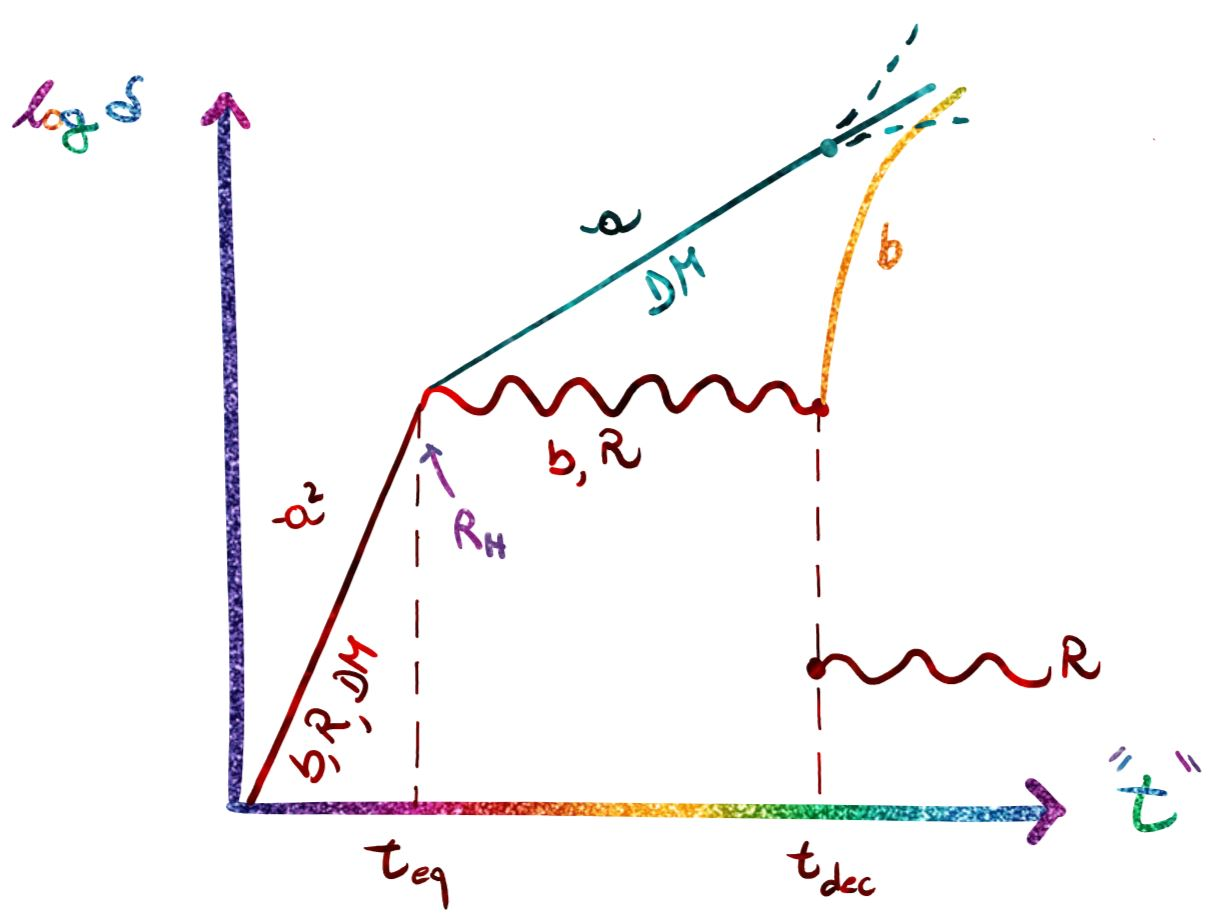
\includegraphics[width=.8 \textwidth]{Pictures/6/dmgrowingfactor.jpg}
    \caption{non fidarsi delle concavità}
\end{figure}


\subsection{Sommario}

\begin{figure}[H]
    \centering
    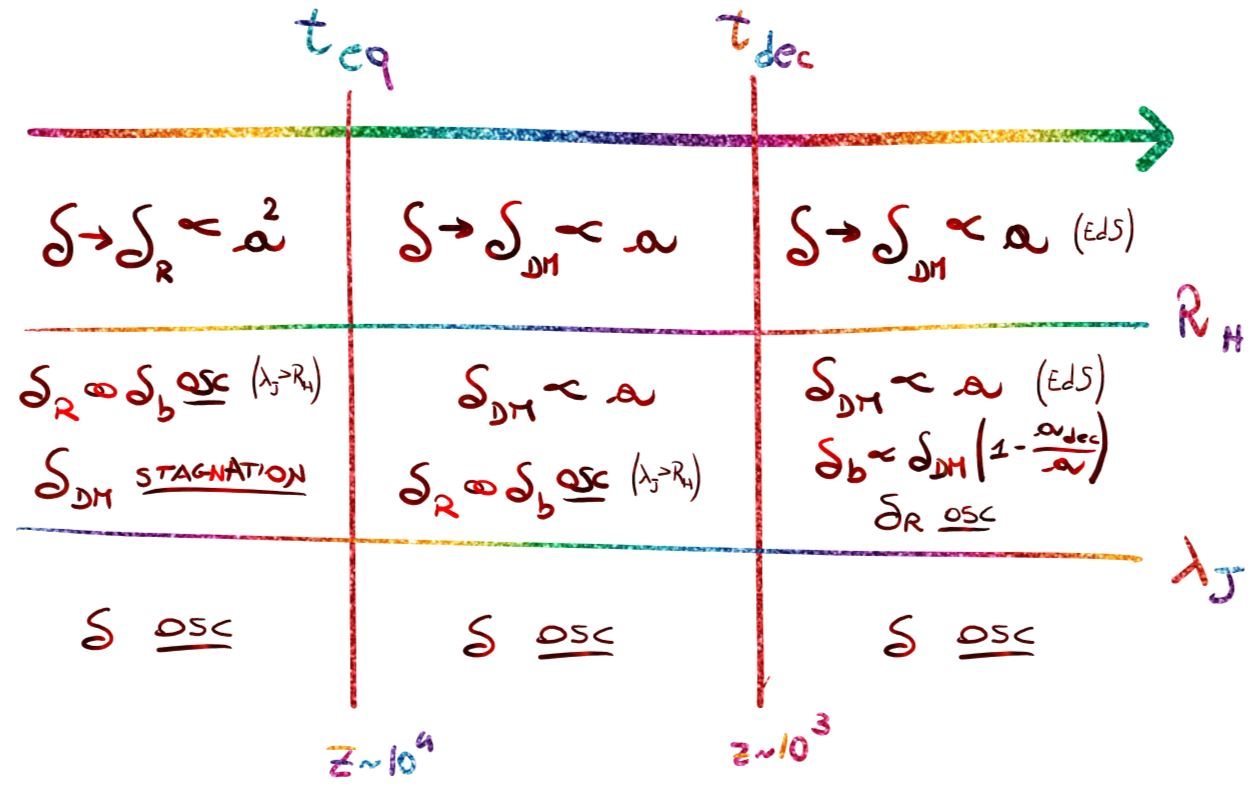
\includegraphics[width=\textwidth]{Pictures/6/sommario.jpg}
    \caption{Riassunto delle soluzioni trovate per il modello di Jeans per un universo in espansione. Mentre per $t<t_{dec}$ è ragionavole aver assunto EdS, la presenza della costante cosmologica può alterare le dipendenza per i tempi successivi ($\delta_{DM}^{close}\propto > a$, $\delta_{DM}^{open}\propto < a$). }
\end{figure}
\chapterimage{/7/head.jpg} % Chapter heading image
\chapter{Un'oscillazione non è per sempre}\label{7:ch}

\subsection{Hot N Cold Dark Matter}
Da un punto di vista cosmologico, l'interesse principale non è nella/e particella/e costituenti la materia oscura, ma nei suoi effetti. In particolare deve interagire debolmente con la materia barionica e con sé stessa (da cui la categoria delle \textit{Weakly Interacting Massive Particles}). Data una nuova particalla teorizzata, e.g. il \textit{laurino}, i cosmologi vorrebbero sapere:
\begin{enumerate}
    \item Massa: definisce a grandi linee il momento in cui la particella smette di essere relativistica, dall'uguaglianza $k_B T = m_xc^2$. Le particelle che smettono di essere relativistiche più tardi sono quelle via via più leggere.
    \item Interazione con fluido radiativo e altre particelle: definisce il tempo di disaccoppiamento con le altre componenti $\tau = (n_x c \sigma)^{-1}$.
\end{enumerate}

Si definiscono particelle di \textbf{materia oscura calda (HDM)} quelle ancora relativistiche al momento del disaccoppiamento dal fluido: $\tau_{dec,x}<\tau_{nRel}$. Tipico candidato è il neutrino, con la sua massa estremamente piccola. Quelle per cui vale la relazione inversa sono particelle di \textbf{materia oscura fredda (CDM)}. Vanno quindi confrontati tre tempi fondamentali: $\tau_{dec,x}$, $\tau_{nRel}$, $\tau_{eq}$. 
Come si è visto il disaccoppiamento delle particelle di materia oscura avviene nell'era radiativa. La massa di una particella che diventa non relativistica a $t_{eq}$ è:
$$
z_{eq}\simeq 10^4; \quad T_{eq}\simeq 3\cdot 10^4 \: K \quad \rightarrow \quad m_x\simeq 1\: eV
$$
Tutte le particelle con massa più grande di $1\: eV$ (sostanzialmente tutte a parte il neutrino, $m_\nu\simeq few\:\cdot 0.1\: eV$) si sono già de-relativizzate prima dell'equivalenza.

\vspace{1em}

La differenza tra HDM e CDM è da ricercarsi nel fatto che la scala di Jeans dipende dalla velocità della particella e la HDM era ancora relativistica al momento del disaccoppiamento. Per ambedue, il massimo della scala di Jeans è raggiunto al momento dell'equivalenza e vale:
\begin{equation}\left.
    \def\arraystretch{1.3}
        \begin{array}{llll}
        HDM & M_J (t_{eq}) \simeq 10^{15} M_\odot\\
        CDM & M_J (t_{eq})\lesssim 10^{5\div 6} M_\odot
    \end{array}\right.
\end{equation}

Una perturbazione su scala maggiore di $M_J$ può crescere, in particolare tutte le scale maggiori di $M_J(t_{eq})$ crescono sempre. Viceversa, le scale minori, crescono oscillano e \stkout[.5pt]{ricrescono} vengono cancellate (paragrafo successivo). Ovviamente questo discorso ha senso entro l'orizzonte, fuori le perturbazioni crescono sempre. I calcoli della massa di Jeans nei tre (quattro per la CDM) tempi fontamentali sono riportati nella Sezione \ref{ch7:complementi}, gli andamenti sono illustrati nella Figura \ref{fig7:mjhotncold}.

\begin{figure}[H]
    \centering
    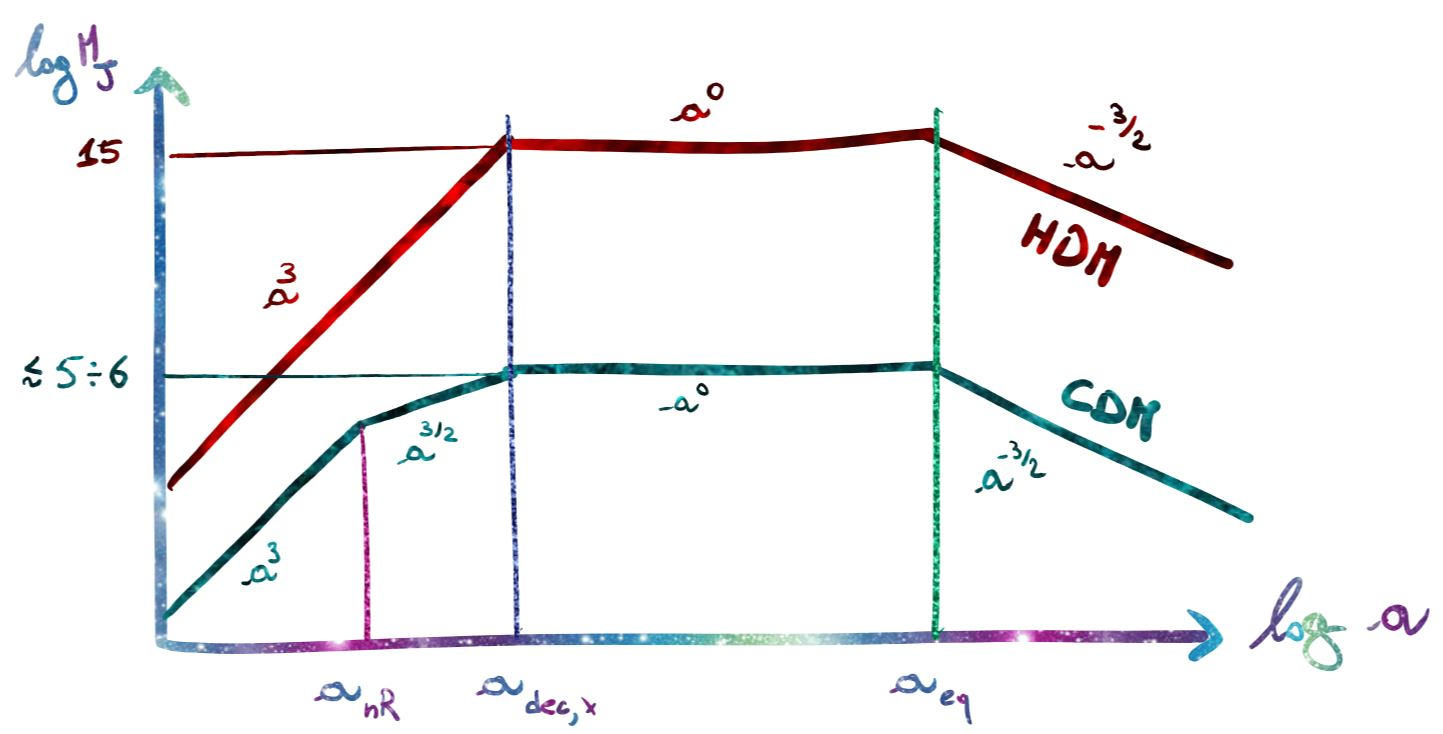
\includegraphics[width=.88 \textwidth]{Pictures/7/mjhotncold.jpg}
    \caption{Evoluzione della massa di Jeans per HDM e CDM al variare del parametro di espansione (tempo).}\label{fig7:mjhotncold}
\end{figure}

\subsection{Massa di Jeans dei barioni}
Viene definito un redshift equivalente a $z_{eq}$, ma per soli barioni: $z_{eq,b}: \; \rho_b=\rho_r$, inserendo la rispettiva dipendenza della densità dal redshift si ottiene:
\begin{equation}
    1+z_{eq,b}=\frac{\Omegabo}{\Omegaro}\simeq 3.9\cdot 10^4\; \Omegabo h^2
\end{equation}

Il disaccoppiamento avviene dopo aver raggiunto l'equivalenza in densità barionica ($z_{dec,b}<z_{eq,b}$) soltando per valori di $\Omegabo h^2 > 0.028$. Planck ha misurato $\Omegabo h^2 = 0.022$. Dato che il valore discriminante è molto vicino a quello misurato, si considereranno entrambi i casi. Gli andamenti nei diversi periodi in esame sono calcolati nella Sezione \ref{ch7:complementi} e illustrati nella Figura \ref{fig:7mjbar}. Si ricorda che sono in esame perturbazioni di tipo adiabatico. Il massimo della scala di Jeans è raggiunto al momento dell'equivalenza/disaccoppiamento e vale:
\begin{equation}\left.
    \def\arraystretch{1.3}
        \begin{array}{l}
     M_{J,b} (t_{dec}) \simeq 10^{16} M_\odot\\
    \end{array}\right.
\end{equation}
\begin{figure}[H]
    \centering
    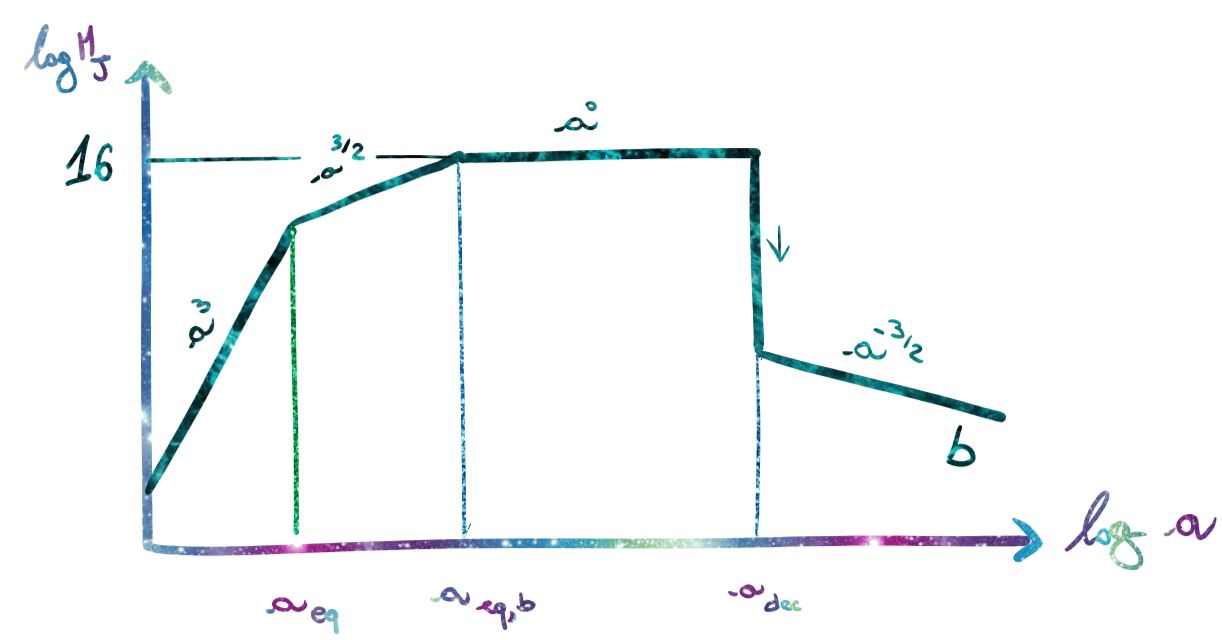
\includegraphics[width=.9 \textwidth]{Pictures/7/mjbar.jpg}
    \caption{Il salto nella normalizzazione è dovuto al fatto che viene a mancare il supporto della radiazione.}\label{fig:7mjbar}
\end{figure}

\section{Materia oscura e \textit{free streaming}}
La particella di materia oscura classica non è collisionale. Per questo motivo di parla di \textit{free streaming} e non di dissipazione. Le particelle, di fatto, rispondono al potenziale medio (quello dell'universo omogeneo), il quale tende a ri-livellare i contrasti di densità. Si definisce \textbf{scala di free-streaming}:
$$
\lambda_{fs}(t) = a(t)\int_0^t \frac{v_{DM}(t')\d{t'}}{a(t')}
$$

Gli andamenti risultanti sono calcolati nella Sezione \ref{ch7:complementi}, inoltre l'evoluzione di $M_{fs}$ è confrontata con $M_J$ nella Figura \ref{fig:7mfscold}. Stando a quanto visto, sotto la scala di Jeans le onde di densità si propagano, ciononostante le scale via via raggiunte da $\lambda_{fs}$ vengono cancellate.

\begin{figure}[H]
    \centering
    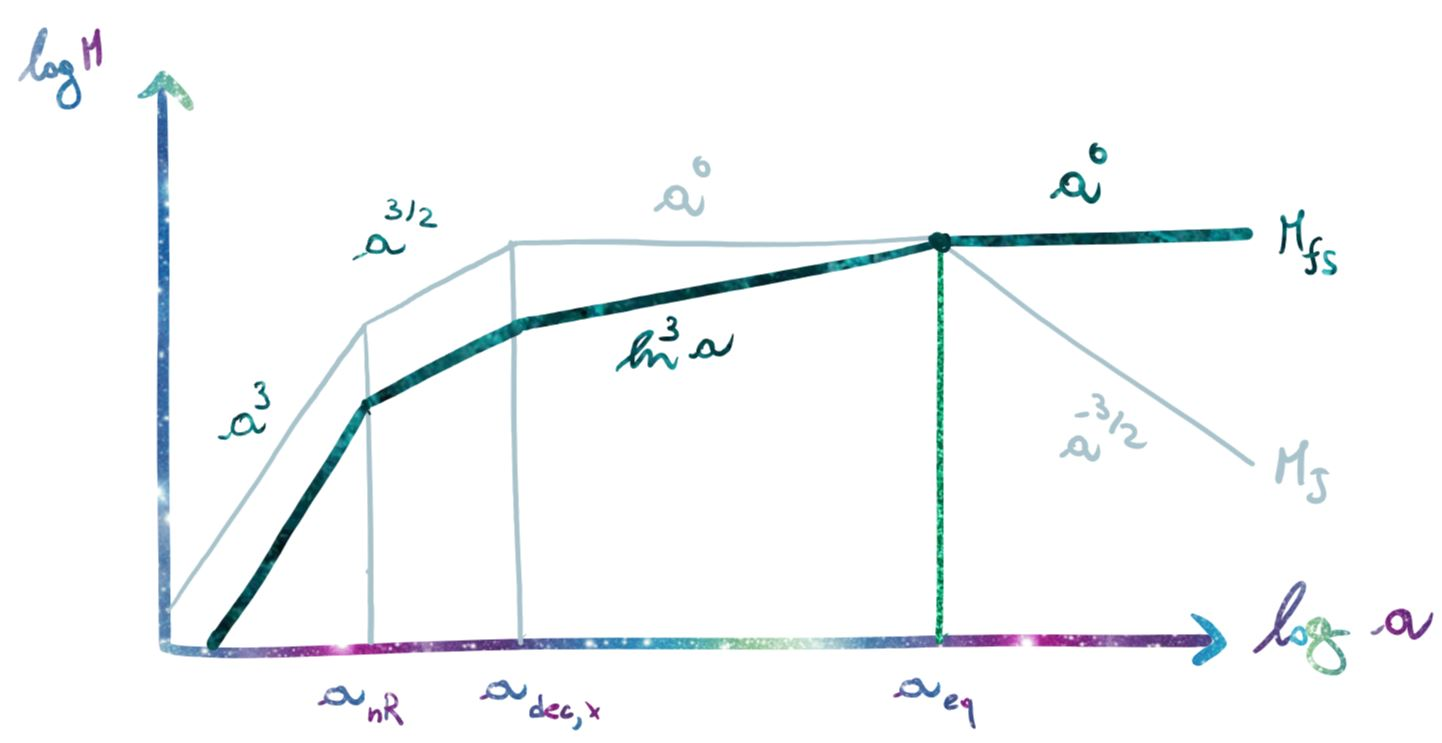
\includegraphics[width=.9 \textwidth]{Pictures/7/mfscold.jpg}
    \caption{Evoluzione di $M_{fs}$ confrontata con $M_J$ normalizzate in $a_{eq}$, si può dimostrare matematicamente che $M_J(t_{eq})=M_{fs}(t_{eq})$. Per definizione la $M_{fs}$ (come il raggio dell'orizzonte) non può decrescere, al massimo rimane costante.}\label{fig:7mfscold}
\end{figure}

\begin{theorem}[Messaggio da portare a casa]
 Dall'equivalenza in poi sopravvivono soltanto le perturbazioni su scala $>M_J$ e poiché $M_J(t_{eq})=M_{fs}(t_{eq})=cost\;\; \forall t>t_{eq}$, tutte le perturbazioni su scale minori non oscillano, vengono \textbf{cancellate}.
\end{theorem}

\vspace{1em}
Nel caso della HDM si ha $M_J(t_{eq})\sim 10^{16}M_\odot$, per cui strutture più piccole (come galassie, ammassi globulari e cose di questo tipo) si devono essere per forza formate per frammentazione di megapalle. Questo scenario è detto \textbf{top-down} (o modello antigerarchico) e prevede che le strutture più grandi siano più vecchie di quelle piccole. Lo scenario alternativo, che ora va per la maggiore, è il \textbf{bottom-up} (o modello gerarchico). Esso richiede particelle di materia oscura fredda e prevede, al variare della loro massa, un valore di $M_J(t_{eq})\sim 1\div 10^{6}M_\odot$. In questo caso si formano prima le strutture piccole, poi per merging gravitazionale quelle più grandi. 

Osservando gli aloni di materia oscura si ha evidenza che questi sono più giovani delle galassie, in accordo col modello gerarchico degli aloni. Quello che succede dentro le galassie è più complesso perché entra in gioco la microfisica del gas (si osserva un comportamento antigerarchico, Thomas et al. 2005)

\newpage
\section{Materia barionica e dissipazione}
In questo caso, e solo in questo caso, si può parlare di scala di dissipazione. In particolare, ci sono due processi che riguardano i barioni: 
\begin{enumerate}
    \item Il libero cammino medio del fotone che si porta dietro il barione $\propto 1/n$ (tende a cancellare le perturbazioni su scale più piccole di $\lambda_{mfp}$);
    \item Lo scattering di fotoni che tende a far perdere coerenza alle onde di perturbazione (dissipazione per urti), come il cammino di un ubriaco.
\end{enumerate}
Il primo è più efficiente perché si oppone alla gravità, il secondo è casuale (?). La scala più grande sotto la quale viene cancellata la perturbazione è:
\begin{equation*}
   \d{x^2} = N_{urti}\lambda_{mfp}^2 = \frac{c\: \d{t}}{\lambda_{mfp}}\lambda_{mfp}^2  = c\: \lambda_{mfp}(t)\d{t}; \qquad \lambda_{mfp}(t)\propto (\sigma_T\rho_b)^{-1}\propto a^{3}
\end{equation*}

Sostituendo i dovuti andamenti di $a$ col tempo e introducendo come massa-scala la cosiddetta \textbf{massa di Silk} si ha:
\begin{equation}x \propto a^\beta \qquad \beta=\left\{
    \def\arraystretch{1.5}
        \begin{array}{llll}
        5/2 & a<a_{eq} & \rightarrow & M_{Silk}\propto a^{9/2} \\
        9/4 & a>a_{eq} & \rightarrow & M_{Silk}\propto a^{15/4}
    \end{array}\right.
\end{equation}

Dopo il disaccoppiamento il libero cammino medio è infinito e non si dissipa più nulla. In questo caso gli andamenti sono diversi da quelli della scala di Jeans, inoltre si ha 
\begin{equation}
    M_{Silk}(t_{dec})\simeq 10^{12}M_\odot
\end{equation}

Per cui, a differenza della materia oscura, la dissipazione non avviene per tutte le scale sotto a $M_J(t_{dec})$, ma esiste un intervallo di scale $\sim 10^{12}\div 10^{16}M_\odot$ in cui le oscillazioni non vengono cancellate e riscrescono dopo $t_{dec}$. Lo spettro delle perturbazioni viene modificato in maniera diversa in funzione della scala (Fig. \ref{fig:7msilkbar}). 
\begin{figure}[H]
    \centering
    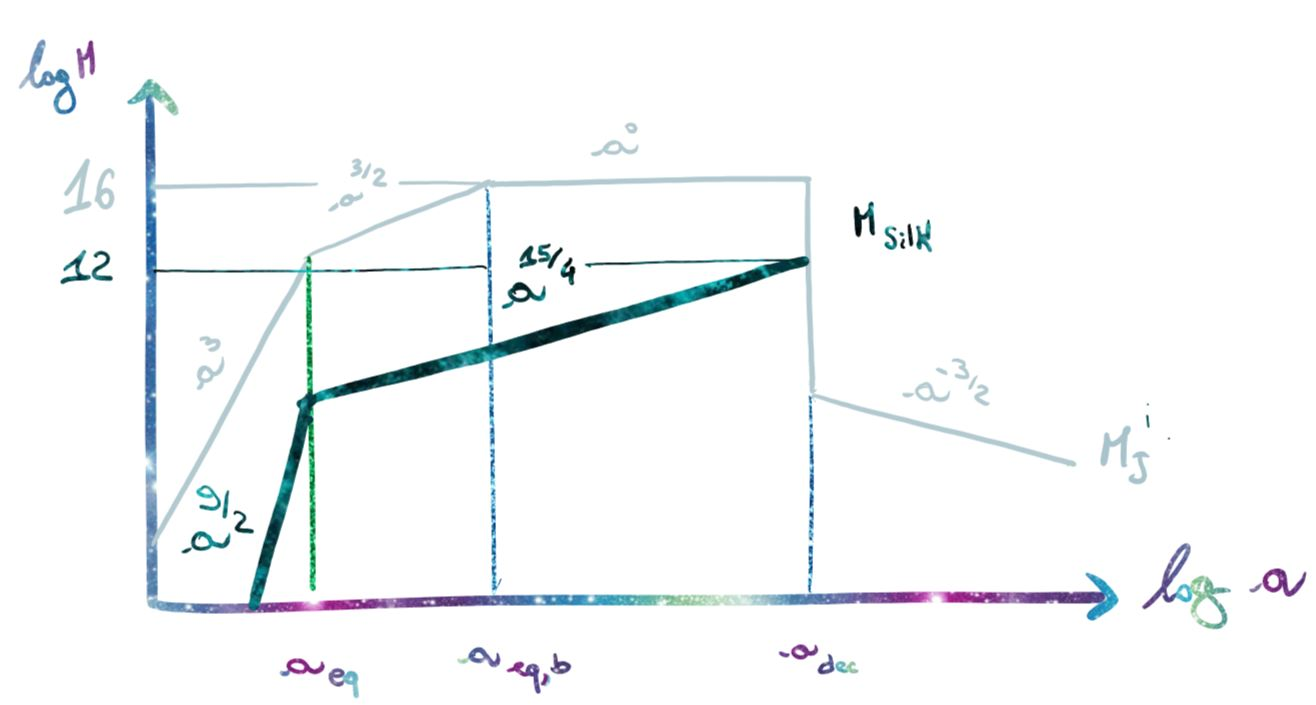
\includegraphics[width=.95 \textwidth]{Pictures/7/msilkbar.jpg}
    \caption{Evoluzione di $M_{fs}$ confrontata con $M_J$ con le dovute normalizzazioni. Per definizione la $M_{Silk}$ (come il raggio dell'orizzonte) non può decrescere, al massimo rimane costante.}\label{fig:7msilkbar}
\end{figure}



\newpage
\section{Complemento: Scale di Jeans, \textit{free streaming} e dissipazione}\label{ch7:complementi}

Per ottenere gli andamenti dalla scala di Jeans e di \textit{free streaming} della \textbf{materia oscura} è necessario ricordare:
\begin{itemize}
    \item $\lambda_J = v_{part}/\sqrt{G\rho}$
    \item $\rho$ è quella della componente dominante ($\propto a^{-4}$ prima di $t_{eq}$ e $\propto a^{-3}$ dopo)
    \item Dalla teoria di Jeans cosmologica $v\propto a^{-1}$ nel caso di moto libero senza processi dissipativi
    \item $M_J\propto \lambda_J^3 a^{-3}$
    \item La definizione di $\lambda_{fs}$
\end{itemize}

\begin{equation}\left.
    \def\arraystretch{1.5}
        \begin{array}{c|llllll}
         & v^2 & \lambda_{J,DM} & M_{J,DM} & \lambda_{fs}& M_{fs} & \\ \midrule
        a < a_{nRel} & c^2/3 & \propto a^2  & \propto a^3 & \propto a^2 & \propto a^3  & \\
        a_{nRel}< a < a_{dec,x} & \propto a^{-1} & \propto a^{3/2} &  a^{3/2} & \propto a^{3/2} & \propto a^{3/2} & (CDM) \\
        a_{dec,x}< a < a_{eq} & \propto a^{-2}  & \propto a & cost & \propto a\ln a & \propto \ln^3 a& \\
        a > a_{eq} & \propto a^{-2} & \propto a^{1/2} &  a^{-3/2} &\propto a  & cost &
    \end{array}\right. \label{tab:7jfsdm}
\end{equation}

\vspace{2em}
Per ottenere le dipendenze dalla scala di Jeans e della \textbf{materia barionica} è necessario ricordare:
\begin{itemize}
    \item I punti ricordati 15 cm fa
    \item $c_s^2=p/\rho$
    \item Per $a_{eq}$ si intende ovviamente $a_{eq,DM}$
\end{itemize}
\begin{equation}\left.
    \def\arraystretch{1.5}
        \begin{array}{c|lllll}
             & c_s^2 & \lambda_{J,b} & M_{J,b} & M_{Silk} & \\ \midrule
        a<a_{eq} & cost & \propto a^2 & \propto a^3 & \propto a^{9/2} &\\
        a_{eq} < a<a_{eq,b} & cost &  \propto a^{3/2} & \propto a^{3/2} & \propto a^{15/4} & \\
        a_{eq,b} < a < a_{dec,b} & \propto a^{_1} & \propto a & cost & \propto a^{15/4} & (se\; esiste) \\
        a > a_{dec,b} & \propto a^{-2} & \propto a^{1/2} & \propto a^{-3/2} & &
    \end{array}\right.  \label{tab:7jbar}
\end{equation}   % 
\chapterimage{/8/head.jpg} % Chapter heading image
\chapter{Statistica con un oggetto}\label{8:ch}

\section{Proprietà Stocastiche delle Perturbazioni}
L'approccio statistico all'analisi delle perturbazioni si basa sulla quantità: $\delta (\vec{x}) = \left (\rho(\vec{x})-\overline{\rho} \right)/\overline{\rho}$ definibile per ogni punto dell'universo, ma della quale interessano principalmente le propietà medie. Il campo $\delta (\vec{x})$ deve essere invariante per traslazioni e rotazioni in base ai principi di omogeneità e isotropia. Da un punto di vista fisico, il campo è generato alla fine della fase inflazionaria (spiraleggiamento nel piano $\phi,\dot{\phi}$) da fluttuazioni statistiche della metrica (verrà assunto rumore bianco). Pertanto il valore $\delta (\vec{x_1})$ non è correlato in fase con $\delta (\vec{x_2})$ e la distribuzione dei valori di $\delta$ può essere assunta \textit{pressoché} gaussiana. Le rappresentazioni nello spazio di Fourier di questi campi, determinano una quantità fondamentale: $\langle \delta k^2 \rangle $.

Ipotesi ergodica: non potendo fare le medie su tante realizzazioni dell'universo (ne esiste una sola), le si fanno su sottospazi sufficientemente grandi e separati (tali da essere indipendenti, \textit{fair sample}) dell'unica realizzazione. Si può dimostrare che per una distribuzione gaussiana, l'ipotesi ergodica è un teorema. Oggi un \textit{fair sample} per avere omogeneità e isotropia si raggiunge a raggi $\gtrsim 100$ Mpc, questa scala diminuisce col tempo essendo l'universo meno strutturato. 

Una gaussiana $P(\delta)$ è definita univocamente da media e varianza, tutti i momenti dispari sono nulli e tutti i momenti pari sono potenze della varianza. Per definizione $\langle \delta \rangle =0 $. Il valore $\delta$ viene espresso nello spazio di Fourier:
\begin{equation}
    \delta{(\vec{x})}=\frac{1}{(2\pi)^3}\int \delta{(\vec{k})}\; e^{i\vec{k}\cdot\vec{x}}\; \d{^3 \vec{k}} \qquad \longleftrightarrow \qquad \delta{(\vec{k})}=\int \delta{(\vec{x})}\; e^{-i\vec{k}\cdot\vec{x}}\; \d{^3 \vec{x}}
\end{equation}
dove $k=2\pi/\lambda$, $\delta{(\vec{x})}$ è adimensionale, $k=[L^{-1}]$ e $\delta{(\vec{k})}=[L^3]$. Essendo un contrasto di densità, è necessario che $\delta{(\vec{x})}\in \mathbb{R} $, per cui per $\delta{(\vec{k})}\in\mathbb{C} $ deve valere: $\delta^*(\vec{k})=\delta{(-\vec{k})}$. Verranno ora introdotte alcune definizioni strategiche.

\vspace{2em}
\begin{example}[Delta di Dirac tridimensionale]
    (\textit{eh iniziamo ad avere troppi delta, ma dopotutto come potremmo chiamarla diversamente?})
    \begin{equation}
        \delta_D^{(3)}(k)= \frac{1}{(2\pi)^3} \int e^{-i\vec{k}\cdot\vec{x}}\; \d{^3 \vec{x}}\qquad \rightarrow\qquad \int f(\vec{k}) \delta_D^{(3)}( \vec{z}-\vec{k} )\d{^3 \vec{k}}= f(\vec{z})
    \end{equation}
\end{example}

\begin{example}[Funzione di correlazione a due punti]
    Indica come il campo correla con sé stesso (\textit{autocorrelazione}) in punti che distano $\vec{r}$ tra loro. È una media su tutti i punti dell'universo e su tutte le direzioni, infatti si sottintende che $\vec{r}=r\hat{n}$ (principio di isotropia). Questo sarà l'osservabile statistico principale per studiare il clustering.
    \begin{equation}
        \xi (r) := \langle\delta (\vec{x}) \delta(\vec{x}+\vec{r}) \rangle 
    \end{equation}
    \begin{equation}
        \xi (r)= \frac{1}{(2\pi)^6}\int \d{^3\vec{k}}\int \d{^3\vec{k'}}\; \langle \delta (\vec{k}) \delta(\vec{k'})\rangle \; e^{ik(\vec{x}+\vec{r})}\; e^{i\vec{k'}\cdot \vec{x}}\label{eq:8xi}
    \end{equation}
\end{example}
Da cui si deriva la teza definizione fondamentale.

\begin{example}[Spettro di potenza]

    \begin{equation}
        \mathcal{P}(k): \quad \langle \delta (\vec{k}) \delta(\vec{k'})\rangle = (2\pi)^3 \mathcal{P}(k)\; \delta_D^{(3)}(\vec{k}+\vec{k'})\label{eq:8pi}
    \end{equation}
    Anche riscrivibile utilizzando la richiesta: $\delta^*(\vec{k})=\delta{(-\vec{k})}$. A differenza della $\xi(r)$, questa quantità è definita nello spazio di Fourier. Inserendola nell'Equazione (\ref{eq:8xi}) si ottiene:
    \begin{equation}
        \xi (r) = \frac{1}{(2\pi)^3} \int \d{^3\vec{k}}\; \mathcal{P}(k)\; e^{i\vec{k'}\cdot \vec{r}}
    \end{equation}
    Questa relazione rappresenta il \textbf{teorema di Wiener–Khintchine}: la funzione di correlazione a due punti $\xi (r)$  e lo spettro di potenza $\mathcal{P}(k)$ sono una coppia di Fourier. Pur essendo $\xi (r)$ più facile da maneggiare in quanto appartenente allo spazio reale, $\mathcal{P}(k)$ è legato al $\delta (k)$ studiato nella teoria lineare e pertanto non se ne scampa. Infatti si può osservare che: $\mathcal{P}(k)\propto \langle\delta^2 (\vec{k})  \rangle $, ossia all'ampiezza quadratica media dell'onda con vettore d'onda $\vec{k}$. Volendo essere rigorosi, è una densità di potenza, la \textbf{potenza delle fluttuazioni} è adimensionale e vale: $\mathcal{P}(k)\d{^3 \vec{k}}$.
\end{example}

Come accennato in precedenza, per principio di isotropia, è conveniente passare alle coordiate sferiche, ricordandosi che $\int \d{^3 \vec{k}}=\int_0^{2\pi}\d{\varphi}\int_0^\pi\d{\theta}\sin\theta\int_0^\infty k^2\d{k}$. La relazione \ref{eq:8pi} modificata per $k=k'$ diventa:
\begin{equation*}
    \langle | \delta_k |^2 \rangle = (2\pi)^3 \; \mathcal{P}(k) \; \delta_D^{(3)}(0) = \mathcal{P}(k) \; V_\infty 
\end{equation*}
dove $V_\infty$ è il \textit{volume infinito}, un infinito formale che rappresenta l'intero volume di integrazione, il volume su tutto lo spazio. Pertanto si ha:
$$
\mathcal{P}(k)  \propto \langle | \delta_k|^2 \rangle
$$
Questo mostra, come precedentemente accennato, che lo spettro di potenza è legato al valore quadratico medio delle ampiezze delle perturbazioni sulla scala $k$. Nel caso di perturbazioni gaussiane, entra in gioco la varianza. 

\subsubsection*{Teorema di Parseval}
Siano $f$ e $g$ due funzioni a valori complessi in una dimensione, si ha che (dimostrabile dalle definizioni precedenti):
\begin{equation*}
    \int^{+\infty}_{-\infty} f(x)g^*(x)\d{x} = \frac{1}{2\pi} \int^{+\infty}_{-\infty} \widetilde{ f}(k)\widetilde{g}^*(k)\d{k}
\end{equation*}
Ossia l'integrale su tutto lo spazio reale del prodotto $f(x)g^*(x)$ è proporzionale all'integrale del prodotto delle due trasformate di Fourier. Per passare in tre dimensioni è sufficiente sostituire $2\pi\rightarrow (2\pi)^3$. 

\subsubsection*{Varianza del campo}
La varianza del campo di densità assunto gaussiano è: $\sigma^2 = \langle  \delta^2 (\vec{x}) \rangle$. Se si divide l'universo in regioni indipendenti e sufficientemente grandi da essere rappresentative, si può calcolare la varianza tramite una doppia media: la media su tutti i volumi della media spaziale quadratica di $\delta$:
\begin{equation*}
    \sigma^2 = \frac{1}{V_\infty} \int \langle  \delta^2 (\vec{x}) \rangle\; \d{^3\vec{x}} \qquad \rightarrow \qquad \sigma^2 = \frac{1}{(2\pi)^3} \int \mathcal{P}(\vec{k}) \; \d{^3\vec{k}}
\end{equation*}
Dove la seconda relazione è ottenuta con il Teorema di Parseval e rappresenta la \textbf{varianza puntuale}, ossia la somma dei contributi della potenza per ogni scala $k$ (è un'informazione globale/integrata). Da un punto di vista fisico è la potenza ricevuta complessivamente dal campo di densità. In coordinate sferiche diventa: $\sigma^2 =(2\pi)^{-1} \int  k^2\;\mathcal{P}(k)\; \d{k} $. 

Differentemente, $\delta (x)$ vorrebbe essere un'infomazione puntuale, ma provateci voi a calcolare la densità in un punto... non ha senso! Pertanto lo si fa mediandola entro un dato volume. La quantità è \textit{centrata} e non \textit{puntuale} e il campo si dice \textit{filtrato}.

\subsubsection*{Convoluzione}
Il ``filtraggio'' è svolto mediante l'operazione di convoluzione che è così definita:
\begin{equation*}
    [f*g](x) = \int_{-\infty}^{+\infty}f(x-y)g(y)\d{y}
\end{equation*}
Inoltre valgono le proprietà: $f*g=g*f$ e $h(x)=f*g\rightarrow h(k)=f\cdot g$, ossia l'operazione di convoluzione nello spazio di Fourier diventa un semplice prodotto. 

\subsection{Varianza di massa}
Nella pratica, per calcolare la densità, vanno definiti un punto e un raggio entro cui svolgere il conto. Inizialmente, si definisce il contrasto di massa dato una funzione filtro $W((\vec{x}),R)$ come:
$$
\frac{\delta M}{\overline{M}}(\vec{x}) = \delta_M(\vec{x}) = \delta (\vec{x}) * W(\vec{x}, R)
$$
$W$ (da \textit{window}) può essere top-hat $\sqcap $, gaussiano e così via. Questa quantità può essere ricondotta a conteggi di oggetti cosmici (o \textit{tracers}) entro un dato volume $V$:
$$
\frac{\delta N_t}{\overline{N_t}}(V) = \frac{N_t-\overline{N_t}(V)}{\overline{N_t}(V)}
$$
In genere si assume che la distribuzione dei traccianti sia una buona rappresentazione della distribuzione della materia oscura ivi presente. Per escludere effetti di feedback si usano prevalentemente gli ammassi di galassie. Nel caso delle galassie si introduce un fattore $b$ (\textbf{fattore di bias}) e si assume una relazione lineare tra le due quantità: $\delta_{N_g} = b \delta_M$.

Assumendo $\delta (\vec{x})$ gaussiano ($\Rightarrow \delta_M$ gaussiano) si può definire la \textbf{varianza di massa}:
\begin{equation}
    \sigma_M^2 :=  \langle  \delta_M ^2 \rangle = ... = \frac{1}{(2\pi)^3}\int \d{^3\vec{k}}\; \mathcal{P}(\vec{k}) \; W^2(\vec{k}, R)
\end{equation}
Un filtro di questo tipo è un passa-basso (cerca di livellare le disomogeneità tagliando le frequenze più alte). Aumentando la scala su cui si filtra ($R$), le disomogeneità locali (sulle frequenze più alte) vengono tagliate. Ossia, all'aumentare di $R$ passa meno segnale. In particolare si ha:
\begin{equation}
    \sigma_M^2 \xrightarrow[R\to 0]{} \sigma^2 \; (puntuale); \qquad \sigma_M^2 \xrightarrow[R\to \infty]{} 0 \label{eq8:sigmamvsr}
\end{equation}

È abbastanza chiaro che $R\propto k^{-1}\propto M^{1/3}$, quindi si può anche dire di filtrare una data massa.

\section{Spettro di potenza e relazioni di scala}
Si assume uno spettro di potenza del tipo $\mathcal{P}(k) = A k^{n}$, dove $n$ in questo caso è un indice spettrale di tipo scalare (le onde gravitazionali sono rappresentabili con un indice tensoriale). Per $n=0$ tutte le scale in $k$ hanno lo stesso valore di $\mathcal{P}(k)$, per $n>0$ i $k$ grandi (perturbazioni su scale piccole) hanno più potenza (ovvero, ci sono più disomogeneità sulle scale piccole). Questa forma degli spettri di potenza è detta \textit{scale-free}, non prevede scale privilegiate. Per questo motivo l'assunzione sarà valida solo per le condizioni iniziali, ossia in seguito all'inflazione.

La varianza puntuale per questo spettro può avere problemi di convergenza:
\begin{equation} \sigma^2 = \frac{A}{(2\pi)^2}\int_0^\infty  k^{2+n} \d{k} \quad converge \quad \leftrightarrow \quad n\; \left\{
    \begin{array}{ll}
    \leq -3 & k\rightarrow 0 \\
    \geq3 & k\rightarrow \infty
\end{array}\right.
\end{equation}

La varianza di massa diventa:
\begin{equation}
    \sigma_M^2 \propto \int \d{^3 \vec{k}}\; k^n\; W^2(k,R)
\end{equation}

Eventuali deviazioni dall'andamento di $\mathcal{P}(k)$ rispetto a quanto assunto, vengono visualizzate meglio con l'indice spettrale effettivo:
\begin{equation}
    n_{eff}=\frac{\d{\ln \mathcal{P}(k)}}{\d{\ln k}}
\end{equation}
che rappresenta in corrispondenza della scala $k$ la pendenza locale dello spettro.

\subsection{Relazioni di scala non lineari}\label{8:sec:relnlin}
Si può utilizzare la teoria lineare per predire i comportamenti delle relazioni di scala degli oggetti formati, che sono chiaramente in regime non lineare. In questo regime le perturbazioni evolvono con un fattore di crescita $\delta_+ (t)$ indipendente dalla scala, conseguentemente lo spettro iniziale verrà moltiplicato per un fattore $\delta_+^2 (t)$. Trascurando il filtro:
$$
\sigma_M^2 \quad\propto\quad \delta_+^2\; k^{n+3} \quad\propto\quad \delta_+^2\;  R^{-(n+3)} \quad\propto\quad \delta_+^2\;  M^{-(n+3)/3}
$$
La teoria lineare è valida finché $\sigma_M^2 \propto \delta^2 = 1$, per cui ponendo $\sigma_M^2 =1$ si definiscono le scale $k$ che diventano non lineari a un certo tempo $t$. Assumendo EdS per l'era della materia:
\begin{equation}\left\{
    \def\arraystretch{1.5}
        \begin{array}{l}
        M_* \propto (1+z)^{-6/(n+3)} \\
        t_* \propto M_* ^{(3+n)/4} \\
        R_* \propto (1+z)^{-1}\\
        \langle \sigma_*^2 \rangle = M_*^{(1-n)/6}
    \end{array}\right. 
\end{equation}
dove $t_*$ rappresenta il tempo tipico di formazione di un oggetto con massa $M_*$, $R_*$ la sua dimensione. Queste sono le relazioni di scala non lineari tra gli osservabili delle strutture formate, valide quando la gravità è l’unica forza ad
aver influenzato la formazione. (Se la gravità fosse l'unica ad agire, una galassia dovrebbe essere esteticamente uguale a un ammasso di galassie, globulare, eccetera). 

\vspace{1em}
\noindent Per avere \textbf{clustering gerarchico} è necessario porre due contraints:
\begin{enumerate}
    \item La formazione gerarchica (tempi piccoli = masse piccole) delle strutture richiede: $$n>-3$$
    \item L'energetica deve crescere al crescere della massa (non solo per semplice aggregazione): $$n<1$$
\end{enumerate}
Nello scenario della CDM l'indice spettrale sta dentro questo range. Volendo, le stesse leggi di scala possono essere ricavate per un universo non-EdS. Purtroppo includendo la microfisica, iniziano comunque a traballare.

\section{Spettro di Zeldovich}
L'inflazione preferisce:
$$
\mathcal{P}(k) = Ak^n; \qquad n=1
$$
che viene detto \textbf{spettro di Zeldovich}. Deriva dall'assumere che le perturbazioni vengono generate in modo stocastico dall'oscillazione dell'inflatone e che sono rumore bianco (non hanno scale privilegiate).  A grandi linee, le fluttuazioni di un campo gravitazionale su scala $R$ hanno un andamento del tipo: $\delta \phi (R) \propto \delta \rho \; R^2 \propto \sigma_M R^{3/2} \propto M^{(1-n)/6}$, pertanto per ottenere una relazione \textit{scale-free} si deve avere $n=1$. In realtà, l'indice spettrale dipende dal potenziale e dalle sue derivate e la relazione per l'inflazione esatta è:
\begin{equation}
    n_{infl}=1+2\eta -6\epsilon \simeq 0.96
\end{equation}
dove $\eta$ ed $\epsilon$ sono gli stessi del paragrafo (CITAAAAAAAA) ed è proprio studiando la forma dell'indice spettrale che possono essere misurati. Inoltre vi è una leggera dipendenza dalla scala (una forma del potenziale leggermente diversa determina un'uscita anticipata o ritardata dall'inflazione). Planck, misurando $n_{infl}$ e $\d{n_{infl}}/d{k}$ ha bocciato svariati modelli cosmologici.

\subsection{Ingresso nell'orizzonte}
L'eventuale ingresso nell'orizzonte di alcune scale può deformare lo spettro primordiale. Per un universo EdS la crescita del raggio dell'orizzonte è: $R_H\propto a^\beta$, con $\beta = 2$ prima dell'equivalenza e $\beta =3/2$ dopo. Pertanto, anche la massa contenuta all'interno dell'orizzonte ha un andamento: $M_H\propto a^\beta$ con rispettivamente $\beta=3$ e $\beta=3/2$. In questo modo si può stabilire il tempo a cui una data massa entra nell'orizzonte e conseguentemente, il comportamento della varianza in massa all'entrata nell'orizzonte:
\begin{equation}\left\{
    \def\arraystretch{1.5}
        \begin{array}{llll}
        \sigma_M (z_H) = \sigma_M (z_i) \left(\frac{a}{a_{i}}\right)^2\propto \sigma_M (z_i)  M_H^{2/3} & per & a < a_{eq} &  (\delta_+ \propto a^2) \\
        \sigma_M (z_H) = \sigma_M (z_i) \left(\frac{a_{eq}}{a_{i}}\right)^2\left(\frac{a}{a_{eq}}\right)\propto \sigma_M (z_i)  M_H^{2/3} & per & a > a_{eq} &  (\delta_+ \propto a)
    \end{array}\right. \label{eq8:primadopoh}
\end{equation}
dove il pedice $i$ rappresenta i valori prima dell'ingresso e $a=a_H$ il valore del parametro di espansione all'ingresso. Queste relazioni mostrano che l'altezza delle perturbazioni al tempo di entrata nell'orizzonte ha gli stessi andamenti, indipendentemente dal fatto che questa avvenga prima o dopo l'equivalenza. In particolare, ricordando che $\sigma_M \propto M^{-(3+n)/6}$ si ha: 
$$
\sigma_M (z_H) \propto M^{(1-n)/6}
$$

Riassumendo, assumere lo spettro di Zeldovich per le fluttuazioni primrdiali implica che:
\begin{enumerate}
    \item Le fluttuazioni del potenziale gravitazionale / della metrica sono completamente indipendenti dalla scala (\textit{white noise});
    \item Le perturbazioni di densità possono entrare nell’orizzonte in momenti diversi, ma tutte con la stessa ampiezza.
\end{enumerate}

Per $n\neq1$ si hanno due casi: $n>1 \rightarrow \sigma_M (z_H)\propto M^{<0}$ le perturbazioni di massa minore entrano nell’orizzonte con un'ampiezza maggiore (scenario \textit{bottom-up}), viceversa $n>1 \rightarrow \sigma_M (z_H)\propto M^{>0}$ (scenario \textit{top-down}).

\subsection{Effetto della stagnazione}
Una prima modifica dello spettro di potenza è dovuta all'effetto di stagnazione. Nel momento in cui le perturbazioni entrano nell'orizzonte in epoca precedente all'equivalenza, possono crescere al più di un fattore $5/2$, ossia rimangono costanti. Nel caso di CDM , le perturbazioni che subiranno per più tempo l'effetto di stagnazione sono quelle di più piccola scala (entrano prima nell'orizzonte). In maniera simile a quanto fatto nell'Equazione \ref{eq8:primadopoh} si ricavano due andamenti di $\delta(k,t_{eq})$ dall'istante iniziale $t_i$:
\begin{itemize}
    \item Le scale $k$ che entrano nell'orizzonte quando $a_H <a_{eq}$ subiscono l'effetto di stagnazione: si considera quindi la crescita fino ad $a_H$. $$ \delta (k, t_{eq})\propto \delta (k, t_i) M_H^{2/3} \propto \delta (k, t_i) k^{-2}\qquad\rightarrow\qquad \mathcal{P}(k,t_{eq}) \propto \mathcal{P}_i\; k^{-4}$$
    \item Le scale $k$ che entrano nell'orizzonte quando $a_H > a_{eq}$ non subiscono l'effetto di stagnazione. $$ \delta (k, t_{eq})\propto \delta (k, t_i) \qquad\rightarrow\qquad \mathcal{P}(k,t_{eq}) \propto \mathcal{P}_i$$
\end{itemize}
Come già visto, col passare del tempo il raggio dell'orizzonte cresce e ingloba scale via via sempre più grandi ($k$ piccoli). Lo spettro risultante è riportato in figura \ref{fig8:bella}. Come è possibile notare, l'indice $n$ determina un differente tempo di entrata nell'orizzonte. Assumendo lo spettro di Zeldovich si ha che: $\mathcal{P}(k)\rightarrow k^{n_{eff}}$ con $n_{eff}=-3$ per alti $k$ e $n_{eff}=1$ per piccoli $k$ (come lo spettro primordiale). Questi valori sono compatibili con l'intervallo richiesto per avere clustering gerarchico (Sez. \ref{8:sec:relnlin}).  
\begin{figure}[H]
    \centering
    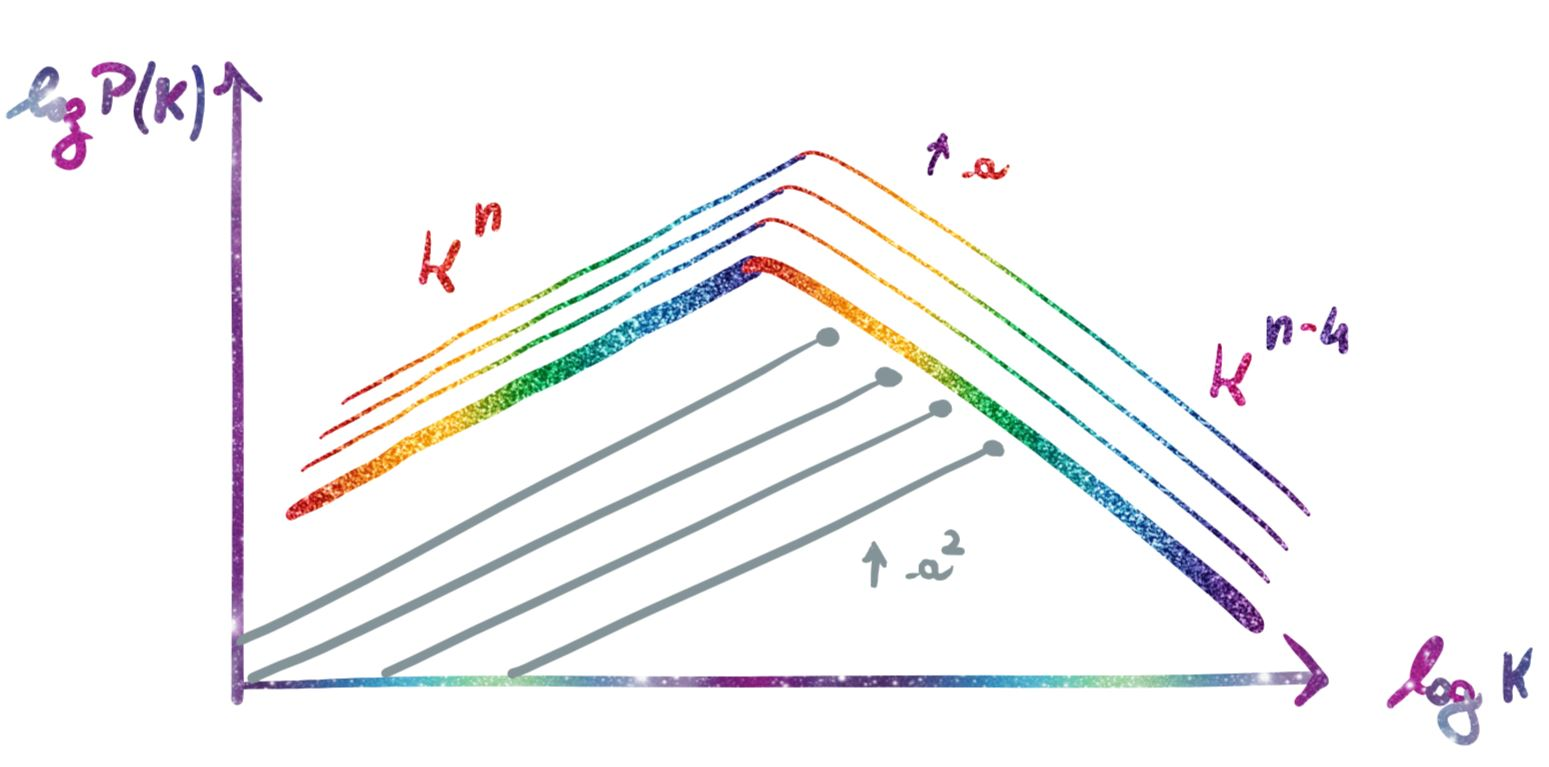
\includegraphics[width=.8 \textwidth]{Pictures/8/pertmatevolnic.jpg}
    \caption{Evoluzione dello spettro di potenza per la materia. In grigio le fasi prima dell'equivalenza: le scale piccole ($k$ grandi) entrano via via nell'orizzonte e stagnano. L'orizzonte si muove verso sinistra $\leftarrowtail $. In arcobaleno glitterato lo spettro al momento dell'equivalenza e successivamente la sua evoluzione autosimilare (come mai il picco si sposta un po' a destra?).} \label{fig8:bella} 
\end{figure}


La scala su cui avviene il turnover corrisponde a quella che entra nell'orizzonte al momento dell'equivalenza $k_{eq}$, pertanto lo spettro di potenza è influenzato anche dal valore di $\Omega_{m0}$. Studiando gli andamenti si ha: $k_{eq}\propto R_H^{-1}(t_{eq}) \propto \dot{a} = a H_0 E = f(H_0,\Omega_{m0})$. Inoltre come visto in precedenza: $1+z_{eq}=\Omega_{m0}/\Omega_{R0}$. Pertanto con più materia l'equivalenza avviene a redshift più alti con la conseguenza che l'orizzonte riesce a inglobare meno $k$: si preserva maggiormente lo spettro primordiale e il turnover si sposta a destra $\rightarrowtail $ (Fig. \ref{fig8:bella2}). Per un ragionamento analogo, all'aumentare della componente radiativa (e.g. neutrini) il picco si sposta a sinistra $\leftarrowtail $. Osservativamente, $k_{eq}\simeq 2\cdot 10^{-2}\; h$ Mpc$^{-1}$.
\begin{figure}[H]
    \centering
    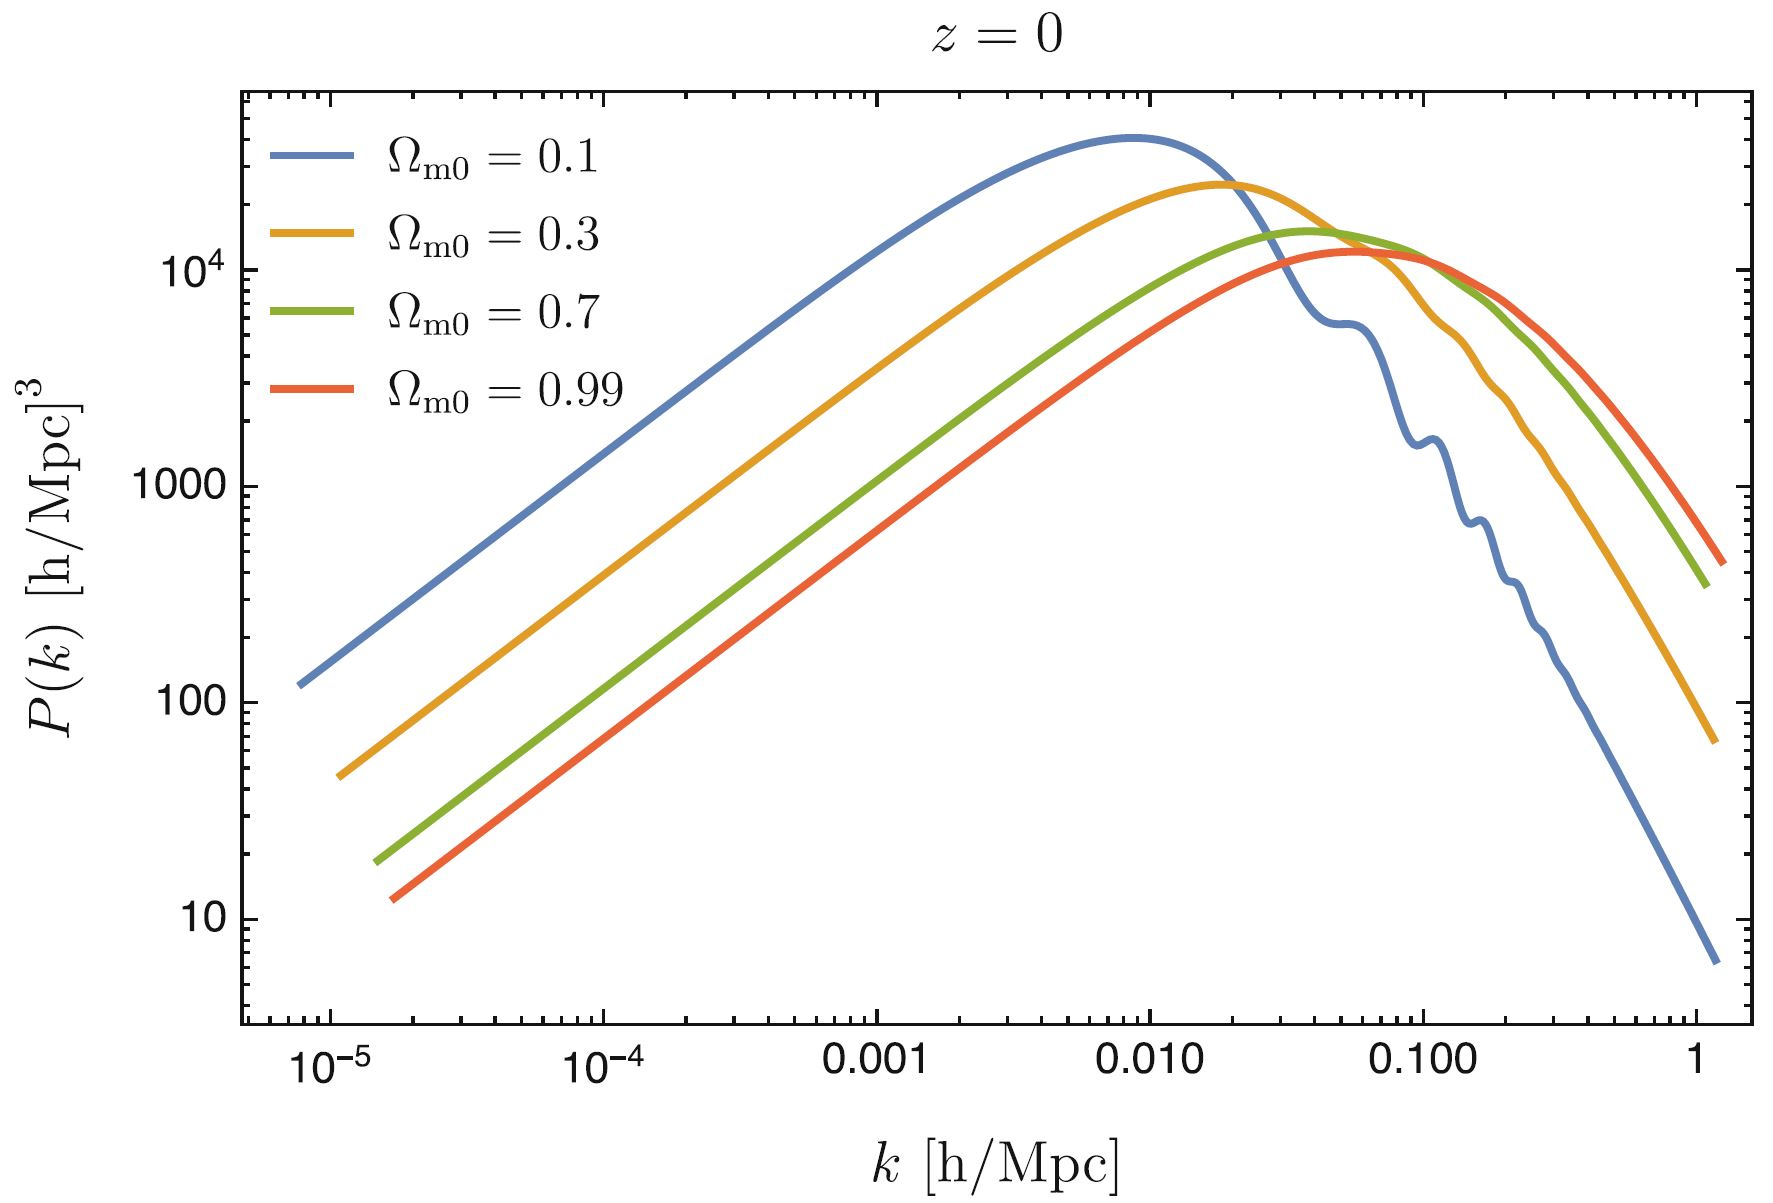
\includegraphics[width=.6 \textwidth]{Pictures/8/pertmatevol.jpg}
    \caption{Spettro di potenza per la materia al variare di $\Omega_{m0}$. Da: Oliver Piattella - \textit{Lecture notes in Cosmology} (Springer, 2018)}\label{fig8:bella2} 
\end{figure}

Per misurare $n$ bisogna osservare la curva per $k<k_{eq}$, che non è modificata dalla microfisica. Gli ammassi di galassie si collocano a destra del picco in corrispondenza $n_{eff}\approx 0$ e in seguito si trovano le galassie con $n_{eff}\approx -1$. Lo spettro osservato tramite survey di galassie e ammassi (Fig. \ref{fig8:bella3}) rigetta il modello HDM (così come fa la CMB). Modelli con $n\neq 1$ sono detti \textit{tilted}, e.g. per $n=0.8$ (meno ripidi) si sposta potenza sulle grandi scale, sfavorendo il collasso di piccole strutture.

\begin{figure}[H]
    \subfloat[]{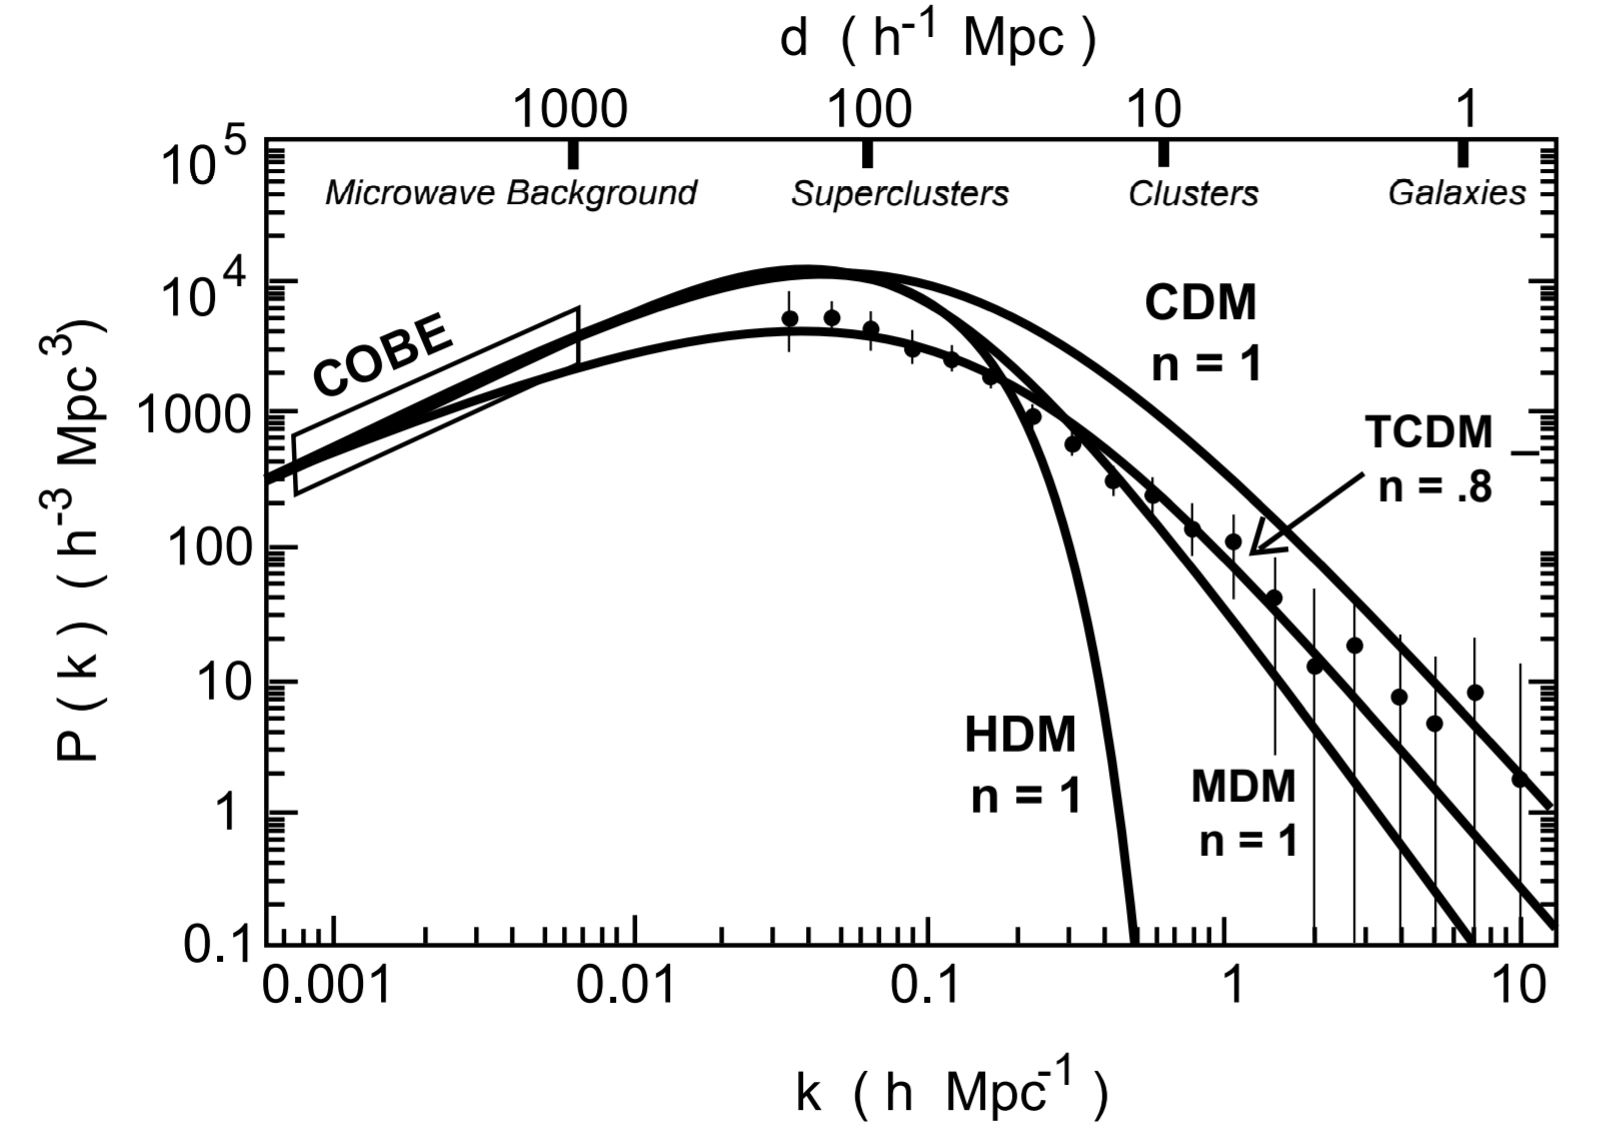
\includegraphics[width=.6\textwidth]{Pictures/8/tris1.jpg}}$\;\;$
    \subfloat[]{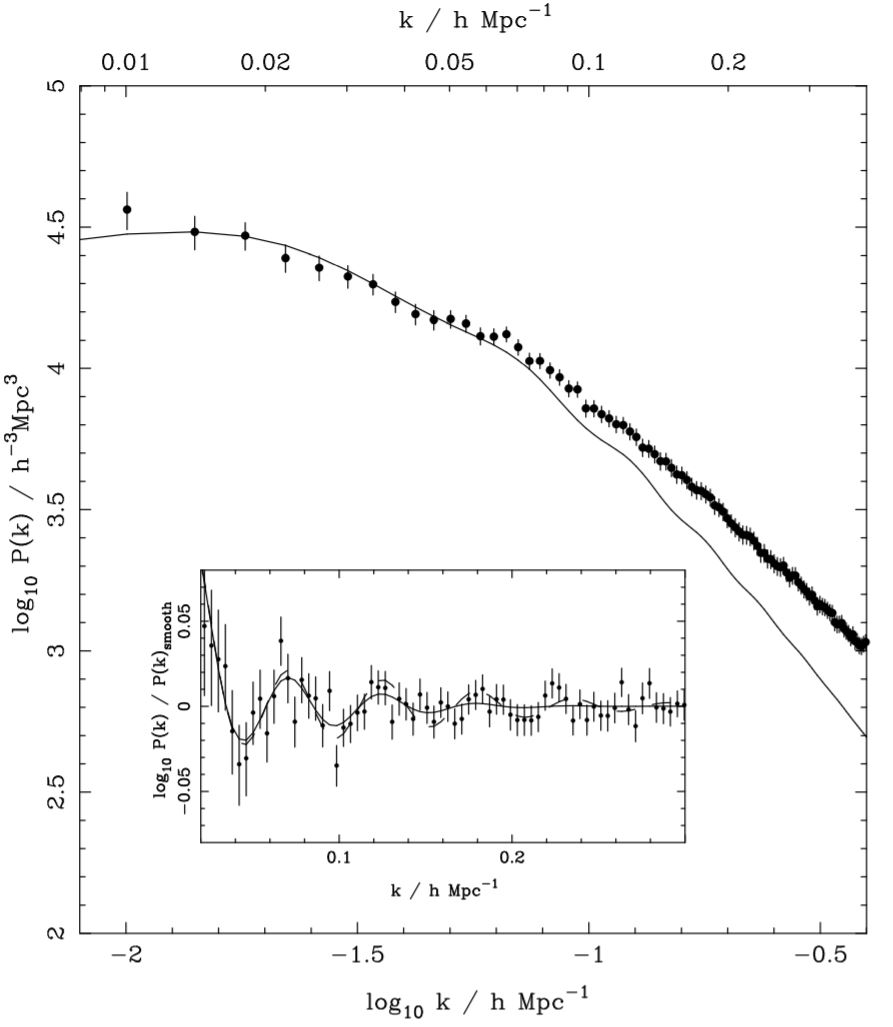
\includegraphics[width=.355\textwidth]{Pictures/8/tris3.jpg}}
    \caption{(a) Modelli di densità di potenza per Hot, Mixed (Warm) e Cold Dark Matter (i punti rappresentano i dati osservati che fittano un modello \textit{tilted}) (From: Kolb - \textit{Particle Physics in the Early Universe}, 1998); (b) Redshift-space power spectrum (notare $k/h$ sulle ascisse) per un campione di galassie (From: Percival et al. - \textit{The shape of the SDSS DR5 galaxy power spectrum}, 2006).} \label{fig8:bella3} 
\end{figure}


\subsection{Effetto del \textit{free-streaming}}
Mediante un'analisi più dettagliata si nota che per il modello HDM la densità di potenza decade per $k$ grandi e il turnover è spostato leggermente a destra rispetto al CDM (questo secondo effetto si notava in un'immagine a bassa qualità che è stata rigettata dall'editore). Questo è dovuto al fatto che $M_{fs, HDM}\simeq 10^{16}M_\odot$ (vs. $M_{fs, CDM}< 10^{6}M_\odot$), pertanto le perturbazioni sono state cancellate per scale maggiori o $k$ più piccoli (il taglio dovuto al free streaming per il modello CDM è fuori dal grafico a destra, non è rilevante cosmologicamente). Inoltre, lo shift a destra del picco è dovuto al fatto che il free streaming è causale e può avvenire solo dentro l'orizzonte. 

Un modo alternativo per visualizzare questo effetto è fare uso della quantità adimensionale $k^3\mathcal{P}(k)$. Ancor meglio, a voler essere precisi, in letteratura si fa uso della quantità:
\begin{equation}
    \Delta^2(k) = \frac{k^3}{2\pi^2}\mathcal{P}(k)
\end{equation}
che è la vera \textbf{potenza} delle perturbazioni (si usa anche la sua radice). Deviazioni dal modello CDM per grandi $k$, possono essere imputate alla presenza di neutrini massicci, pertanto se ne può stimare la loro massa media (misurando da qui $\rho_\nu$ e dalla CMB $N_\nu$). Lo stesso ragionamento vale nel caso di warm dark matter (Fig. \ref{fig8:bella4}).


\begin{figure}[H]
    \centering
    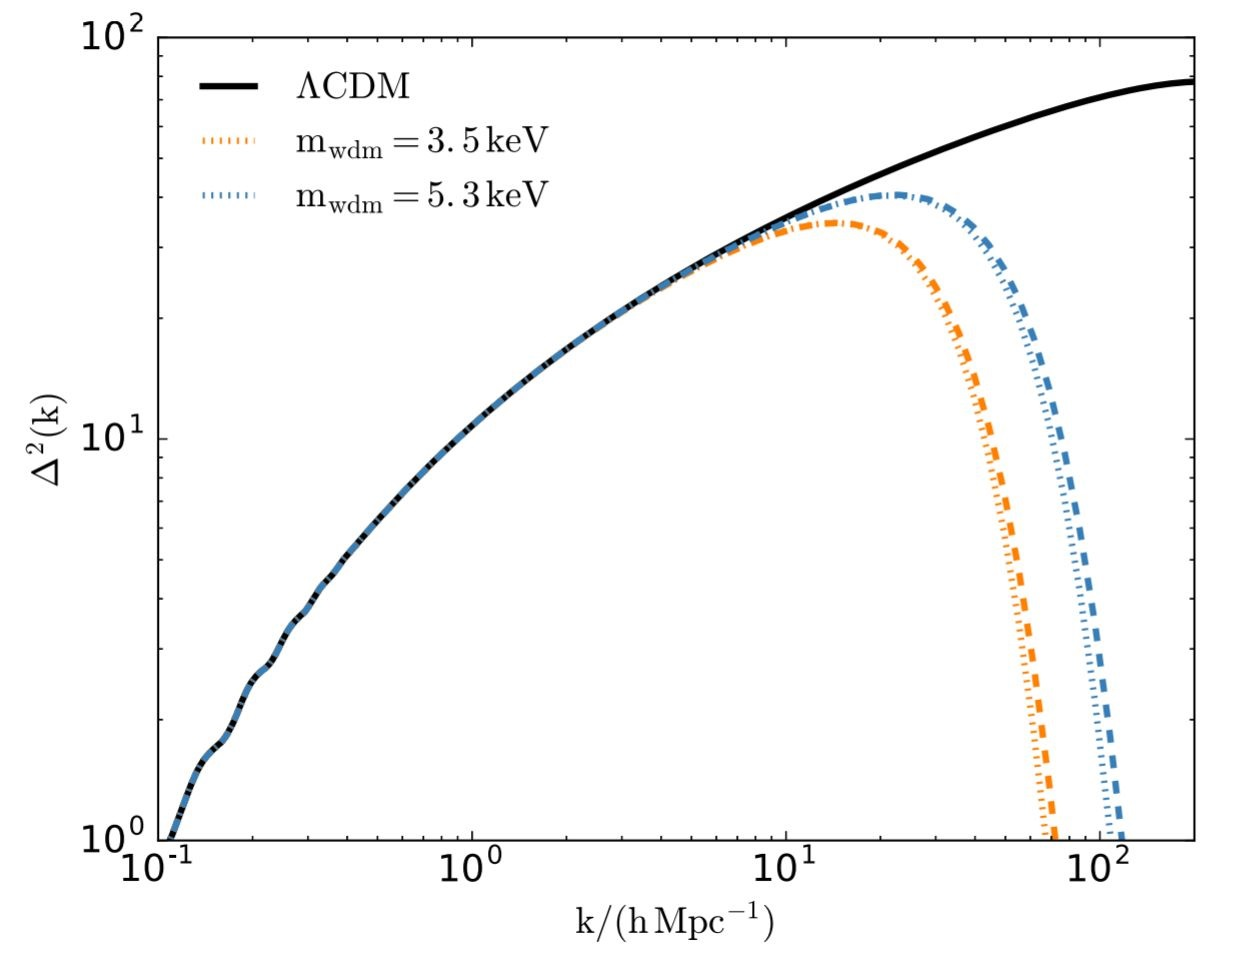
\includegraphics[width=.53 \textwidth]{Pictures/8/tris4.jpg}
    \vspace*{-1em}
    \caption{Spettro di potenza per modelli $\Lambda$CDM e WDM. $\Lambda$CDM: $k^3\mathcal{P}(k)\propto 1$ per $k$ grandi, R e M piccoli; $k^3\mathcal{P}(k)\propto k^4$ per $k$ piccoli, R e M grandi.  (From: Ricaldi et al. - \textit{On general features of warm dark matter with reduced relativistic
    gas}, 2018).} \label{fig8:bella4}
\end{figure}

\begin{example}[Funzione di trasferimento] 
    In letteratura si fa spesso uso della seguente convenzione:
    \begin{equation}
        \mathcal{P}(t_{eq},k)=\mathcal{P}_i(k)\; T^2(k)
    \end{equation}
    dove $T(k)$ è la funzione di trasferimento e nel caso in analisi è costante prima dell'equivalenza ed evolve $\propto k^{-2}$ dopo. Questa quantità dipende molto dalle assunzioni sulla materia oscura (Fig. \ref{fig8:transfun}) e sulla cosmologia, mentre $\mathcal{P}_i$ dipende dal modello inflazionario. Inoltre per il regime non lineare la trattazione viene ulteriormente complicata.

\end{example}
\begin{figure}[H]
    \centering
    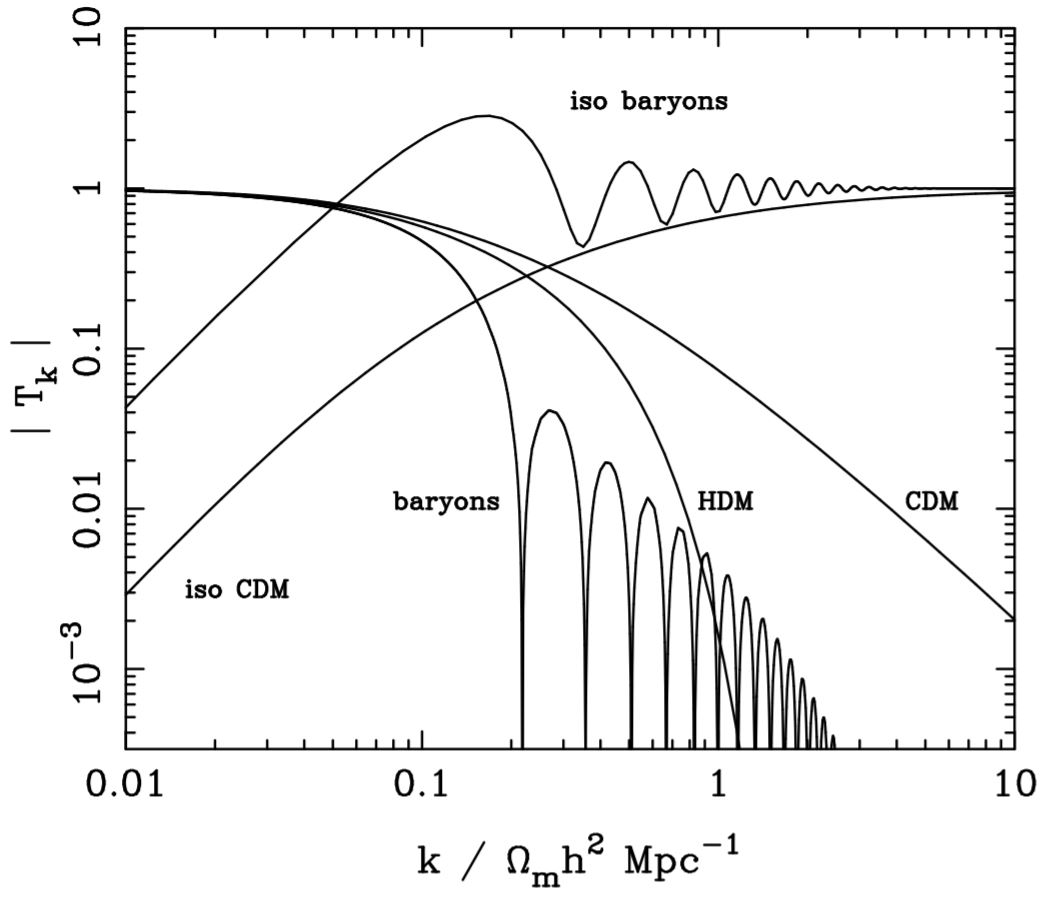
\includegraphics[width=.53 \textwidth]{Pictures/8/transfun.jpg}
    \vspace*{-1em}
    \caption{Funzione di trasferimento per vari modelli Si noti che $T_k\to 1$ a piccoli $k$ per modelli adiabatici e a grandi $k$ per modelli a isocurvatura. Per la dark matter il numero d'onda caratteristico scala proporzionalmente a $\Omega_m h^2$, i barioni hanno un comportamento diverso come verrà discusso a breve. Infine si può notare che la HDM è in difetto di potenza rispetto alla CDM. (From: J.A. Peacock - \textit{Large-scale surveys and cosmic structure}, 2003))}\label{fig8:transfun} 
\end{figure}



\subsection{Evoluzione post-equivalenza}
La figura \ref{fig8:bella} mostra l'evoluzione dello spettro di potenza anche dopo $t_{eq}$ per le assunzioni fino ad ora adottate. La crescita è \textit{autosimilare}. Questo non è più vero quando le perturbazioni diventano non lineari, ossia quando viene raggiunto il valore $\delta, \sigma_M \to 1$. Le scale piccole ($k$ grandi) diventano non lineari prima delle altre (cfr. Eq. \ref{eq8:sigmamvsr}). L’effetto netto è quello di un innalzamento dello spettro a grandi $k$ (Fig. \ref{fig8:ultimabella}).

\begin{figure}[H]
    \centering
    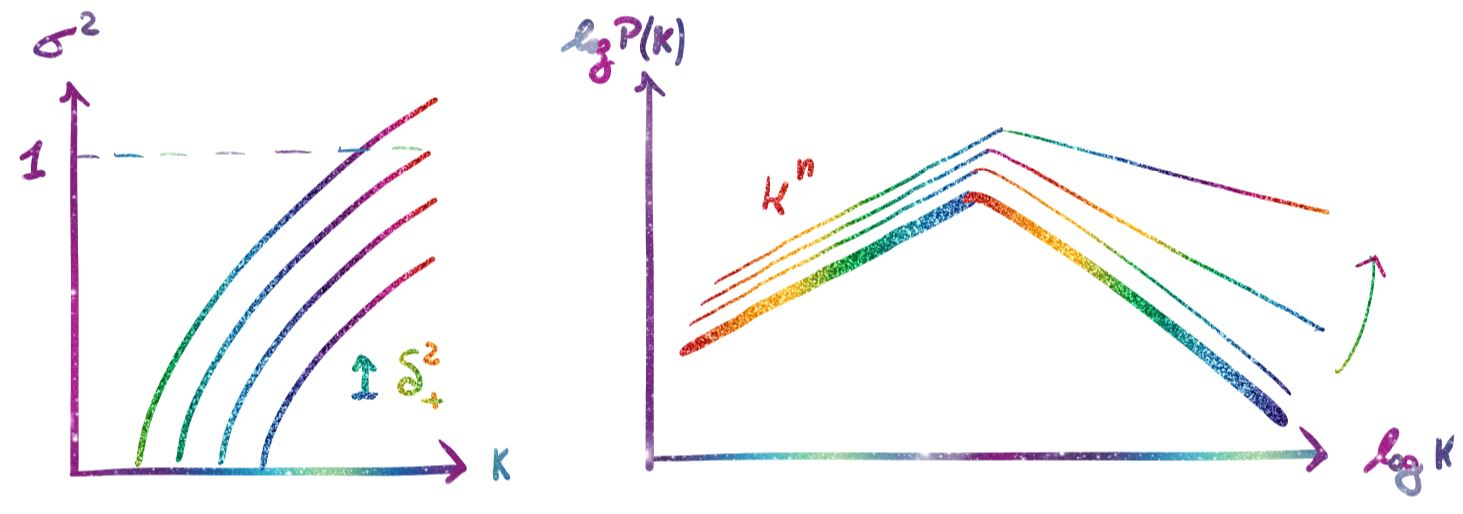
\includegraphics[width=.85 \textwidth]{Pictures/8/truevol.jpg}
    \vspace*{-1em}
    \caption{Sinistra: evoluzione di $\sigma^2$ in teoria lineare, le prime scale a diventare non lineari sono quelle grandi ($k$ piccoli); Destra: Crescita delle perturbazioni in regime non lineare. Lo spettro viene deformato a piccole scale, questo è un altro motivo per cui è meglio studiarlo a  grandi scale.}\label{fig8:ultimabella}
\end{figure}


\section{Distribuzione delle perturbazioni}
Come visto inizialmente si assume una distribuzione delle perturbazioni gaussiana:
\begin{equation}
    P(\delta_M)=\frac{1}{\sqrt{2\pi \sigma_M^2}}e^{-\frac{\delta_M^2}{2\sigma_M^2}}
\end{equation}
purtuttavia esiste un limite fisico per $\delta$ (ossia $\rho \geq 0$):
\begin{equation}
    \delta = \frac{\rho - \overbar{\rho}}{\overbar{\rho}} = \frac{\rho}{\overbar{\rho}}-1 > -1
\end{equation}
La situazione diventa ancora più imbarazzante col tempo perché la gaussiana si allargherebbe ($\sigma_M^2 \to \sigma_M^2 \delta_+^2$) ben oltre il valore limite $-1$. Per ovviare a questo problema si assume che la probabilità si accumuli vicino a $-1$ senza superarlo, rendendo di fatto la distribuzione non gaussiana. Col tempo la gaussiana si abbassa e si allarga, ma lo fa in modo asimmetrico (Fig. \ref{fig8:ultima}). Questa assunzione prevede una grande quantità di regioni sottodense (vuoti), mentre la materia si accumula tutta nei nodi. Questo discorso è valido su scale molto grandi, cioè quelle che hanno mantenuto la distribuzione gaussiana generata all’inflazione e per redshift elevati in cui la crescita è stata lineare su tutte le scale (CMB).

\vspace{1em}
L'\textbf{altezza delle perturbazioni} 
\begin{figure}[h]
    \centering
    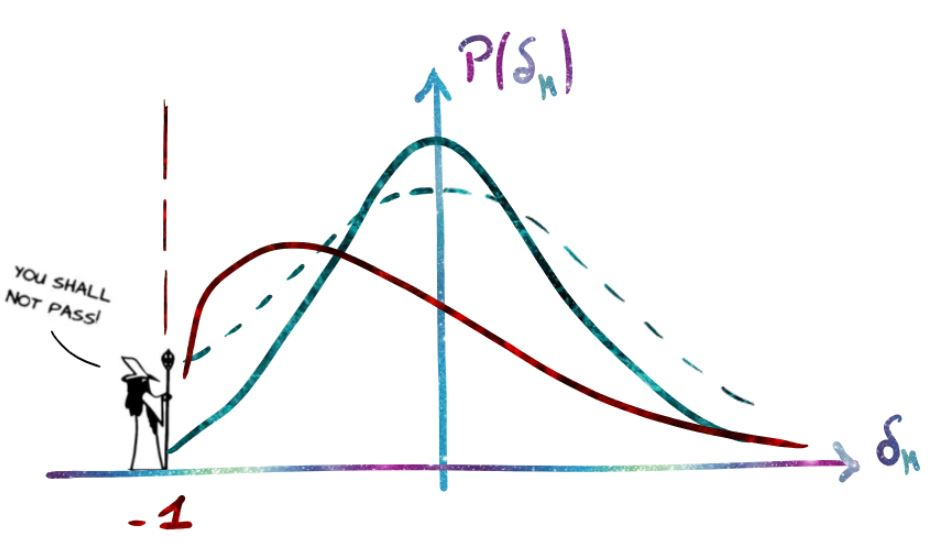
\includegraphics[width=.65 \textwidth]{Pictures/8/pdfevol.jpg}
    \vspace*{-1em}
    \caption{In verde tratteggiato l'evoluzione classica delle perturbazioni gaussiane. In rosso l'evoluzione assunta per evitare valori inferiori a $-1$. L'area sottesa non deve cambiare (=1), pertanto la distribuzione viene distorta.}\label{fig8:ultima}
\end{figure}



Ll'evoluzione di una distribuzione gaussiana è problematica se è richiesto fisicamente $\delta > -1$. Un'alternativa è ricorrere a una distribuzione dei picchi lognormale (P. Coles \& B. Jones, 1991) scegliendo come ansatz $\rho /\overbar{\rho} = 1+\delta_{nLin} \propto e^{\delta_{Lin}}$. La varianza lognormale è legata a quella gaussiana dalla relazione: $\sigma_{nLin}^2 = e^{\sigma^2}-1$, pertanto la funzione di distribuzione di probabilità diventa:
\begin{equation}
    f(1+\delta_{nLin})= \frac{1}{(1+\delta_{nLin})\sqrt{2\pi \ln(1+\sigma_{nLin}^2)}}e^{-\frac{\ln^2\left((1+\delta_{nLin})/\sqrt{1+\sigma_{nLin}^2}\right)}{2 \ln(1+\sigma_{nLin}^2)}}
\end{equation}
Mappando la distribuzione e sfruttanto le proprietà dei campi gaussiani si riduce la complessità delle simulazioni fatte con questo modello.    % Pert
\chapterimage{/9/head.jpg} % Chapter heading image
\chapter{Evoluzione non Lineare}\label{9:ch}
Le osservazioni attuali degli ammassi di galassie suggeriscono valori di $\delta \gg 1$, dell'ordine di $100$ o addirittura $1000$. In questi regimi l'approssimazione lineare non è più valida ed è necessario sviluppare una teoria non lineare adeguata. Seppur in qualche caso si riescano a fare i conti con carta e penna (\textit{regime weakly non-linear}, per studiare meglio l'avvicinamento a $\delta = 1$), il più delle volte sono necessarie simulazioni numeriche. 


\section{Approssimazione di Zeldovich}
Questo approccio per descrivere l'evoluzione non lineare delle perturbazioni prevede una distribuzione iniziale omogenea di materia non collisionale, descritta inizialmente da una lagrangiana imperturbata:
\begin{equation}
    \vec{r}(\vec{q},t)=a(t)\vec{q}+\vec{F}(\vec{q},t) \qquad \rightarrow \qquad \vec{r}(\vec{q},t)=a(t)\left[\vec{q}+\delta_+ (t) \vec{G}(\vec{q})\right]\label{eq9:zelapprox}
\end{equation}
dove $\vec{r}=a(t)\vec{x}$ ($\vec{x}$ coordinata comovente), $\vec{F}(\vec{q},t)$ è il termine di displacement, dipendente solo dalla posizione iniziale (sarà il limite di questo metodo) e si è assunta la separabilità: $\vec{F}(\vec{q},t)=a(t)\delta_+ (t)$ per analogia con la teoria lineare. Inoltre il termine di velocità, che quantifica lo spostamento di una particella rispetto alla posizione iniziale, è legato al potenziale gravitazionale iniziale dalla relazione: $\vec{G}(\vec{q})= -\nabla_q \Phi_0 (\vec{q})$. Inoltre si ha:
\begin{equation*}\left.
    \def\arraystretch{1.8}
        \begin{array}{l}
        \vec{v}=\frac{\d{\vec{r}}}{\d{t}}-H\vec{r}=a\frac{\d{\vec{x}}}{\d{t}}=a\;\dot{\delta}_+\nabla_q \Phi_0 (\vec{q}) \\
        \nabla^2_q \Phi_0 = \delta / \delta_+ (t) \quad\rightarrow\quad \delta = \delta_+ (t)\nabla^2_q \Phi_0  \quad (Eq.\; Poisson)
        
    \end{array}\right. 
\end{equation*}
Nell'approssimazione di Zeldovich pertanto, l'approssimazione lineare è svolta sullo spostamento delle particelle, piuttosto che sulla densità. Viene detta teoria di perturbazione \textit{lagrangiana} al primo ordine (precedentemente si è trattata la teoria di perturbazione \textit{euleriana} al primo ordine). Richiede il calcolo del potenziale soltanto all'istante iniziale e prevede che le particelle si muovano su traiettorie rette. Il modello non è più esatto quando due particelle (assunte non collisionali) si incrociano (shell crossing): si viene a creare una singolatità. L'equazione \ref{eq9:zelapprox} mappa univocamente le coordinate $\vec{q}$ e $\vec{r}$, quindi fintantoché due traiettorie non si incrociano, per piccoli spostamenti si ha:
\begin{equation}
    \rho(\vec{r},t)\d{^3r}=\overbar{\rho} (t_i) \d{^3q} \quad \rightarrow \quad \rho(\vec{r},t) = \frac{\overbar{\rho} (t)}{|J(\vec{r},t)|}
\end{equation}
dove $|J(\vec{r},t)|$ è il determinante della matrice Jacobiana. Dal mometo che il fluido è irrotazionale, la matrice è simmetrica e quindi può essere diagonalizzata:
\begin{equation}
    \rho(\vec{r},t)=\overbar{\rho} (t) \left[\left(1-\delta_+ \lambda_1\right)\left(1-\delta_+ \lambda_2\right)\left(1-\delta_+ \lambda_3\right)\right]^{-1}
\end{equation}
Per tempi sufficientemente piccoli, per cui $\delta_+ (t)\lambda_i\ll 1$, si ha:
\begin{equation}
    \delta\simeq -\left(\lambda_1 + \lambda_2 + \lambda_3\right)\delta_+(t)
\end{equation}
Se i tre autovalori $\lambda_i (\not\propto t)$ sono $<0$ la densità diminuisce, se sono $>0$ la densità cresce, ma può anche verificarsi che diverga all'infinito (\textit{shell crossing}). Nel caso in cui tutti e tre gli autovalori siano uguali si ha espansione/collasso sferico, altrimenti è ellissoidale. Per due negativi e uno positivo collasso planare e per due positivi e uno negativo collasso su un filamento. Questo modello regge bene fino a $\delta\sim 5$, ma può essere sviiluppato a ordini superiori. 
Si può dimostrare che la formazione delle strutture avviene inizialmente su piani (\textit{pancake di Zeldovich}), mentre al passare del tempo sono preferite strutture filamentose che convergono in nodi. 

\section{Collasso sferico}
Si considerano le perturbazioni come universi chiusi immersi in un universo di background EdS e si assume che siano perfettamente sferiche e ferme rispetto al flusso di Hubble $v_{pec}=0$. Nella Sezione \ref{ch6:chilovoleva} era stato ricavato l'andamento delle perturbazioni dopo l'equivalenza che rispetto un generico istante iniziale diventa:
\begin{equation}
    \delta = \delta_+ \left(\frac{t}{t_i}\right)^{2/3} + \delta_- \left(\frac{t}{t_i}\right)^{-1}\label{eq9:delta}
\end{equation}
ora la perturbazione decrescente non viene più trascurata. In regime lineare: $v = ia\dot{\delta}/k_x $, inoltre in un universo EdS: $a\propto t^{2/3}$ (per i tempi in esame). Indicando con il pedice $x$ le coordinate comoventi e con $r$ quelle fisiche ($k_r = k_x /a$) si ha: 
\begin{equation}
    v= \frac{i}{k_x \left(t/t_i\right)^{-2/3}}\;\frac{1}{t_i}\left[ \frac{2}{3}\delta_+ \left(\frac{t}{t_i}\right)^{-1/3} - \delta_- \left(\frac{t}{t_i}\right)^{-4/3}    \right]  
\end{equation}
Applicando l'assunzione $v(t_i)=0$ e l'equazione \ref{eq9:delta} si ha:
$$
\delta_- (t_i)= \frac{2}{3}\delta_+(t_i)\quad \rightarrow \quad \delta (t_i) = \frac{5}{3}\delta_+ (t_i)
$$

Il parametro di densità della perturbazione vale: $\Omega_p(t_i)=\rho_p(t_i) / \rho_{crit} = \Omega (t_i) (1+\delta(t_i))$, dove $\Omega (t_i)$ è il parametro di densità dell'universo di background. La \textbf{condizione per il collasso della perturbazione sferica} è $\Omega_p (t_i)>1$, ossia:
$$
\Omega (t_i) (1+\delta(t_i)) > 1
$$
Se $\Omega (t_i)\geq 1$ tutte le perturbazioni collassano, mentre se $\Omega (t_i)< 1$ si introduce un \textbf{valore di soglia} che deve essere superato affinché si possa avere collasso:
\begin{equation}
    \delta_+ (t_i) > \frac{3}{5}\left(\frac{1-\Omega (t_i)}{\Omega (t_i)}\right)
\end{equation}

La condizione per un universo di background di Friedmann con sola materia diventa:
$$
\delta_+ (t_i) > \frac{3}{5}\frac{1-\Omega_i}{\Omega_i (1+z_i)}
$$
Questo significa che esiste una soglia che va superata in tempo utile (aumenta col tempo) se si vuole avere collasso. Questa è sempre superata in universi chiusi e piatti $\Omega_i \geq 1$, ma non per quelli aperti. L'evoluzione del piccolo universo chiuso con cui è stata approssimata la perturbazione prevede un $t_{max}$ a cui si ha un $a_{max}$, $\dot{a}(t_{max})$ e quindi una successiva contrazione (\textit{big crunch}), inoltre $\rho_p (t_{max})\propto a_{max}^{-3}$. Si può dimostrare che la densità della perturbazione al tempo del massimo vale:
\begin{equation}
    \rho_p (t_{max})=\frac{3\pi }{32\; G} \; \frac{1}{t_{max}^2}
\end{equation}
Confrondola con la densità del background ($\rho(t_{max})=(6\pi \; G \; t_{max}^2)^{-1}$) si ottiene:
$$
\chi (t_{max}):= \frac{\rho_p(t_{max})}{\rho (t_{max})}= \frac{9\pi^2}{16}\approx 5.6 \qquad \rightarrow\qquad \delta^{nLin} (t_{max})= \chi -1 \approx 4.6
$$
ovvero, al momento del \textit{turnaround}, la perturbazione è già altamente non lineare e le assunzioni fatte per questo modello non valgono più. Seguendo puramente la trattazione lineare avremmo ottenuto un valore:
$$
\delta_+^{lin}(t_{max})=\frac{3}{5} \left(\frac{3\pi}{4}\right)^{2/3}\approx 1.07
$$
Il risultato è sbagliato di un fattore 4 e deve ancora iniziare il collasso vero e proprio.



\section{Fase di virializzazione}
Ci si aspetta che la perturbazione, assunta come universo chuiso, ricollassi su sé stessa in un tempo $t_{coll}=2t_{max}$. Tuttavia le perturbazioni di materia non possono collassare in un punto: entrano in gioco il riscaldamento nel caso di materia barionica e la dispersione di velocità nel caso di materia oscura. La perturbazione si virializza su un dato raggio calcolabile dal teorema del viriale:
\begin{equation*}\left\{
    \def\arraystretch{1.5}
        \begin{array}{ll}
            2T+V=0 \\
            E=T+V
    \end{array}\right. \quad\Leftrightarrow  \quad E(t_{vir})=\frac{V}{2}= -\frac{1}{2}\frac{3}{5}\frac{G M^2}{R_{vir}}\equiv E(t_{max})=-\frac{3}{5}\frac{GM^2}{R_{max}}
\end{equation*}
dove si è posto per conservazione dell'energia, $E(t_{vir})\equiv E(t_{max})$, periodo in cui la velocità e quindi l'energia cintica è nulla. Da questa relazione si ha che la perturbazione si virializza quando: $R_{vir}=R_{max}/2$, ossia quando $\rho_p (t_{vir})=8 \rho_p (t_{max})$. Le simulazioni mostrano che il tempo in cui avviene la virializzazione è $t_{vir}\simeq 3 t_{max}$. Con questi dati si possono stimare due quantità fondamentali:
\begin{equation}\left\{
    \def\arraystretch{1.5}
        \begin{array}{ll}
        \frac{\rho_p (t_{coll})}{\overbar{\rho}(t_{coll})}=8 \frac{\rho_p (t_{max})}{\overbar{\rho}(t_{max})}\left(\frac{t_{coll}}{t_{max}}\right)^2 \simeq 180\\
        \frac{\rho_p (t_{vir})}{\overbar{\rho}(t_{vir})}=8 \frac{\rho_p (t_{max})}{\overbar{\rho}(t_{max})}\left(\frac{t_{vir}}{t_{max}}\right)^2 \simeq 400
    \end{array}\right. 
\end{equation}
dove si è utilizzata la quantità $\chi (t_{max})$ calcolata nella sezione precedente. Questi due valori corrispondono a dei $\delta$ (sottraendo 1) decisamente non lineari. Svolgendo ingenuamente i conti con la teoria puramente lineare, si sarebbe ottenuto:
\begin{equation}\left\{
    \def\arraystretch{1.5}
        \begin{array}{ll}
        \delta^{lin}(t_{coll})=\delta^{lin}(t_{max})\left(\frac{t_{coll}}{t_{max}^{2/3}\simeq 1.68\\
        \delta^{lin}(t_{vir})=\delta^{lin}(t_{max})\left(\frac{t_{vir}}{t_{max}^{2/3}\simeq 2.2
    \end{array}\right. 
\end{equation}

\section{Funzione di massa}



\section{Simulazioni numeriche}   % N lin
\chapterimage{/10/head.jpg} % Chapter heading image
\chapter{Clustering}\label{10:ch}
Con il termine \textit{clustering} si intendono le proprietà di distribuzione della materia su grande scala. Il clustering viene studiato in modo statistico: si utilizzano principalmente la funzione di correlazione (Paragrafo CITAAAA) e la sua trasfomata di Fourier. Entro un volumetto $\d{V_1}$ la probabilità di trovarvi un oggetto è $\d{P_1}=\overline{n}\d{V_1}$, dove $\overline{n}$ è l densità media di oggetti. La probabilità congiunta di avere un oggetto in due generici volumi, nel caso in cui le singole probabilità siano completamente indipendenti, vale: $\d{P}_{12}=\overline{n}^2 \d{V_1}\d{V_2}$. L'eccesso o il difetto di probabilità rispetto alla distribuzione casuale che darebbe questo risultato è detta \textbf{funzione di correlazione spaziale a due punti}, $\xi(\vec{r}_{12})$. Assumendo isotropia: $\xi(\vec{r}_{12})=\xi(r)$, pertanto si ha la seguente relazione: 
\begin{equation}
    \d{P}_{12}=\overline{n}^2 \d{V_1}\d{V_2} \left(1+\xi(r)\right)
\end{equation}
Per $\xi = 0$ la distribuzione è uniforme, per $\xi >0$ si parla di \textbf{correlazione} e per $\xi <0$ di \textbf{anti-correlazione}. La funzione di correlazione era già stata definita nel caso continuo come correlazione fra il campo $\delta$ e sé stesso in dui punti distanti $r$: $\xi (r)=\langle \delta (x)\delta(x+r) \rangle $. L'uguaglianza tra le due definizioni si può dimostrare facilemente assumendo che tutte le particelle dell'universo abbiano massa uguale. 

Facendo uso del teorema di Bayes si può riscrivere in generale:
\begin{equation}
    \d{P_{12}}= \d{P}(1,2) = \d{P}(1) \d{P}(2|1)\quad \rightarrow \quad \d{P}(2|1)=\overbar{n}\d{V_2}\left(1+\xi(r)\right)
\end{equation}
ossia la probabilità di avere contemporaneamente le condizioni 1 e 2 (rispettivamente un oggetto in $\d{V}_1$ e un oggetto in $\d{V}_2$) è data dalla probabilità di avere 1 moltiplicata per la probabilità (condizionata) di avere 2 dato 1. Da questo è possibile calcolare il numero medio di oggetti entro una sfera centrata su un oggetto dato (e.g. galassie attorno a noi):
\begin{equation}
    \langle N(<r) \rangle =\int \d{P}(2|1) = \frac{4}{3}\pi R^3 \overbar{n} + 4\pi \overbar{n} \int_0^r \d{r'}r'^2 \xi (r') \label{eq10:nummedioentrosfera}
\end{equation}
dove il secondo termine è quello che rappresenta la deviazione dalla distribuzione aspettata data una densità media e un volume. Osservativamente si è visto che:
$$
\xi(r)\propto \left(\frac{r}{r_0}\right)^{-\gamma} \qquad \xrightarrow[z=0]{} \qquad \xi(r)\propto \left(\frac{r}{5\; Mpc/h}\right)^{-1.8}
$$
dove $r_0$ è detta \textbf{lunghezza di correlazione}. Quindi la probabilità di avere un eccesso di coppie su piccola scala è più grande che su grande scala (la tendenza delle galassie è quella di stare vicine vicine). Questa relazione non può continuare per $r\to \infty$, altrimenti il secondo termine dell'Eq. \ref{eq10:nummedioentrosfera} divergerebbe e non si ritroverebbe la densità media dell'universo. Affiché l'integrali si annulli, ci deve essere un punto in cui la funzione di correlazione diventi negativa. Però non può assumere qualsivoglia valore, la proprietà e definita positiva o al più nulla, quindi:
$$
-1 < \xi(r) < +\infty
$$
In ogni caso il valore di $\xi$ tende a $0$ molto velocemente, è difficile da misurare.

Un'alternativa è utilizzare il cosiddetto \textit{conteggio in celle}. In pratica si divide l'universo in tanti piccoli volumi contenenti al più un oggetto. Il numero medio di oggetti entro il volumetto $i$ sarà: $\langle n_i\rangle = \langle n_i^2\rangle = ... =\langle n_i^n\rangle$.
Il numero medio di oggetti entro una sfera centrata su un oggetto a caso nell'universo vale:
\begin{equation}
    \langle N\rangle_V = \int \d{P}(1) \quad \to \quad \Sigma_i \langle n_i\rangle = \overbar{n}V
\end{equation}
Calcolando anche il momento di ordine 2 è possibile ricavare la varianza dei conteggi $\mu_2= \langle N^2 \rangle - \langle N \rangle^2 $:
\begin{equation}
    \langle N^2\rangle_V := \langle\Sigma n_i\; \Sigma n_j \rangle =\overbar{n}V+ \overbar{n}^2V^2 + \overbar{n}^2\int \d{V_1}\d{V_2}\xi_{12} \quad \to \quad \mu_2 = \overbar{n}V+ \overbar{n}^2\int \d{V_1}\d{V_2}\xi_{12}
\end{equation}
Il termine $\overbar{n}V$ è detto \textbf{shot noise} e prescinde dal clustering, che è invece quantificato dall'integrale da cui è possibile fare misure significative su scale molto grandi. La varianza è aumentata dal termine di shot noise a causa della discretezza degli oggetti (un valore di $3.5$ oggetti non è ammissibile). Definendo il contrasto di densità numerica: $\Delta = N - \langle N \rangle / \langle N \rangle$ si può notare che $ \langle \Delta^2 \rangle \propto (\overbar{n}V)^{-1}_{shot}+ V^{-2}\int \d{V_1}\d{V_2}\xi_{12}$, quindi è meglio lavorare su grandi volumi altrimenti il termine di shot noise diventa elevato.
In conclusione, anziché misurare direttamente $\xi$ si preferisce utilizzare i conteggi in sfere poiché il termine da cui si stima, essendo integrato su grandi volumi, diventa più significativo.

\vspace{1em}
Come in tutte le cose della vita alla fine ci si prende gusto e si definisce la \textbf{funzione di correlazione a tre punti}. Questa quantità è necessaria per studiare le distribuzioni non più gaussiane (come per il regime non lineare) aggiungendo informazioni su eventuali direzioni privilegiate. È definita tramite la relazione:
\begin{equation}
    \d{P(1,2,3)}=\d{^3 P}= \overbar{n}^3 \d{V_1}\d{V_2}\d{V_3}\left(1+\xi_3 (r_{12}, r_{13},r_{23})\right)
\end{equation}
con la condizione ovvia $\vec{r}_{12}+ \vec{r}_{13}+\vec{r}_{23}=0$, le variabili da cui dipende $\xi_3$ sono in realtà due. 
\begin{equation}
    \xi_3 (r_{12}, r_{13}, r_{23}) = \xi_2(r_{12}) + \xi_2(r_{13}) + \xi_2(r_{23})+\xi_3^{connessa} (r_{12}, r_{13}, r_{23})
\end{equation}
L'eccesso di probabilità di trovare un tripletto è artificialmente aumentata dal fatto di avere già una coppia, pertanto questi contributi vanno aggiunti al puro eccesso di trovarne solo 3 (\textit{connessa}). Sappiate che avendo $n$ punti, l'unico modo univoco per definire le proprietà della loro distribuzione è conoscere tutti gli $n-1$-esimi momenti. In cosmologia la prima misura di non gaussianità è stata fatta misurando $\Delta^3$ con  $\xi_3$, al massimo ora si arriva a $\Delta^4$ con  $\xi_4$.

\section{Funzione di Correlazione Angolare}
Le stesse quantità appena definite possono essere proiettate angolarmente sul cielo. La misura del redshift è infatti un'approssimazione della distanza vera degli oggetti, che si muovono rispetto al flusso di Hubble con una velocità peculiare $v_{pec}$ difficilmente isolabile. Utilizzare il redshift come terza dimensione ``sporcherebbe'' l'informazione sulla distribuzione degli oggetti. La \textit{funzione di correlazione a due punti angolare} viene così definita:
\begin{equation}
    \d{P}=n_\Omega^2 \d{\Omega_1}\d{\Omega_2}\left( 1+W(\theta)\right)
\end{equation}
dove $\d{\Omega_1}\d{\Omega_2}$ sono piccoli angoli solidi nel cielo che distano $\theta$. In questo modo non ci si sporca le mani con la distanza. Lo stesso approccio è stato utilizzato ai tempi di Peebles (anni '80) quando si avevano solo survey fotometriche e scarsa informazione spettroscopica sui redshift. Per $z=0$ la funzione di correlazione fittata sui dati $\xi(r)$ assume un'andamento del tipo:
$$
W(\theta)\propto \left(\frac{\theta}{\theta_0}\right)^{-0.8}
$$
ossia, proiettandola, viene resa più uniforme. In realtà, esiste una relazione formale per ottenere la distribuzione angolare data una distribuzione spaziale, l'\textbf{equazione di Limber}. Per ottenerla, si considerano la funzione di luminosità $\phi (L) \d{L}$ e il suo legame con la funzione di magnitudine $\psi (M) \d{M}$:
\begin{equation}
    \phi (L) = \left(\frac{L}{L_*}\right)^{-\alpha}e^{-L/L_*} \qquad\qquad \phi (L) \d{L}=\psi (M) \d{M}
\end{equation}
La probabilità di avere in un volumetto una galassia di data magnitudine è: $\d{P}=\psi (M) \d{M}\d{V}$, la funzione di correlazione a due punti viene formalizzata nella forma:
\begin{equation}
    \d{^2P}=\d{M_1}\d{M_2}\d{V_1}\d{V_2} \left(\psi (M_1)\psi (M_2) + G(M_1, M_2, r_{12})\right)
\end{equation}
Notare la differenza ripetto al capitolo precedente. A questo punto si fanno due assunzioni importanti:
\begin{enumerate}
    \item La dipendenza tra magnitudine e distanza è separabile: $G(M_1, M_2, r_{12})=\psi (M_1)\psi (M_2)\xi (r_{12})$. Ora si che la parentesi può tornare: $(1+\xi (r_{12}))$, anche se i dati osservativi non sono molto contenti (soprattutto negli ambienti densi);
    \item Tutte le galassie hanno uguale luminosità $L_*$ (e magnitudine $M_*$): il flusso limite della survey definisce quindi la distanza limite $D_*$ degli oggetti campionati ($D_{Mpc}=10^{0.2(m-M)-5}$);
    \item L'osservazione avviene su angoli piccoli per evitare problemi di curvatura della volta celeste: $r=D_*\sin x \approx D_* x$ ($r$ è la distanza relativa tra due oggetti osservati, $x$ è l'angolo che formano in cielo e $D_*$ è la distanza limite da noi Disgraziati!).
\end{enumerate}
Il numero di galassie medio entro un angolo solido si può quindi scrivere:
\begin{equation}
    n_\Omega = \int^\infty _0 \d{^3r}\int_{-\infty}^{+\infty}\d{M}\psi (M) f(D_*-D) \doteq D_*^3 \int_0^\infty \d{x}\; x^2 \; \psi(x)
\end{equation}
dove $f(D_*-D)$ è una funzione di selezione pari a $1$ se l'argomento è positivo (oggetti entro la distanza imposta dal flusso limite), $0$ altrimenti (nella realtà la transizione non è così netta). In questo modo data una $x$ si scartano tutti gli oggetti che non hanno più la magnitudine tale da essere osservati. Il secondo integrale è poi inglobato in una funzione solo dipendente da $x$, $\psi(x)$. La funzione di correlazione angolare diventa:
\begin{equation}
    \d{^2P}=D_*^6 \int_0^\infty \d{x_1}\; x_1^2 \; \psi(x_1) \int_0^\infty \d{x_2}\; x_2^2 \; \psi(x_2) \left(1+\xi(r_{12})\right)\d{\Omega_1}\d{\Omega_2}
\end{equation}
dove $r_{12}^2=D_*^2 (x_1^2+x_2^2-2x_1x_2\cos \theta_{12})$. Infine, introducendo le quantità: $x=(x_1+x_2)/2$ e $y=(x_1-x_2)/(x\theta_{12})$ si ottiene la fantastica formula:
\begin{equation}
    W(\theta_{12})=\theta_{12}\frac{\int_0^\infty \psi^2(x)x^5\d{x^5} \int_{-\infty}^{+\infty}\xi(D_*\theta_{12}\sqrt{1+y^2}\d{y})}{\left[\int_0^\infty \psi(x)x^2\d{x} \right]}
\end{equation}
detta \textit{equazione di Limber}. Così come la dispersione di velocità delle stelle nelle galassie, i profili di densità e temperatura dei cluster, il lensing e cose di queso tipo... l'equazione può essere utilizzata in due modi:
\begin{itemize}
    \item Assumendo un modello teorico che produce una distribuzione 3D $\xi$ e utilizzandola direttamente per ottenere il $W$ aspettato da confrontare con le osservazioni;
    \item (come si fa di solito) Deproiettando la $W$ osservata attraverso l'equazione invertita.
\end{itemize}
Per due cataloghi con profondità $D_*'\neq D_*$ (magnitudine limite diversa) la funzione di correlazione scala come:
\begin{equation*}
    W'\left(\theta_{12}=\frac{D_*}{D_*'}\theta_{12}'\right)=\frac{D_*}{D_*'}\; W(\theta_{12})
\end{equation*}
ossia, più è profondo il catalogo, meno è clusterata la funzione di correlazione (si omogenizza la distribuzione). In ogni modo, si mantiene l'andamento di $W$ per caloghi di profondità diverse. Come già anticipato, per $\xi \propto r^{-\gamma}$ si ottiene $W\propto \theta^{-\gamma +1}$.

\section{Risultati osservativi}
Per conoscere la distribuzione di materia dell'universo, si può studiare come varia il numero di oggetti al variare del raggio entro cui sono contenuti. Assumendo raggi sufficientemente grandi, la densità media dell'universo tende a zero e l'Equazione \ref{eq10:nummedioentrosfera} diventa:
\begin{equation}
    \langle N(<r)\rangle \propto \int \xi(r) r^2\; \d{r} \qquad \xrightarrow[z=0]{obs} \qquad \langle N(<r)\rangle \propto r^{1.2}
\end{equation}
Le osservazioni locali suggeriscono un andamento con il raggio elevato alla $\sim 1.2$. Per una distribuzione della materia sferica, planare e monodimensionale (filamento), l'esponente dovrebbe essere rispettivamente: $3$, $2$ e $1$. Questo suggerisce che gli oggetti sono distribuiti prevalentemente su filamenti e su piani. In generale:
\begin{equation}
    \langle N(<r)\rangle \propto r^{3-\gamma}
\end{equation}
dove il valore $3-\gamma$ viene detto indice frattale. In base a quanto ricavato, l'universo si dovrebbe auto-riprodurre su tutte le scale. Questo non si verifica perché, come già discusso, la funzione di correlazione deve diventare negativa. [È auspicabile che l'universo non sia un frattale, altrimenti tutto quello che si è fatto fino ad ora andrebbe a farsi benedire: in una distribuzione frattale non si può definire una densità media].

\vspace{1em}
Per calcolare praticamente la funzione di correlazione si utilizza la sua stessa definizione: eccesso/difetto di probabilità rispetto una distribuzione completamente casuale di avere una coppia di oggetti a distanza $r$:
\begin{equation}
    1+\xi(r)=\frac{DD(r)}{RR(r)}            
\end{equation}
dove $DD(r)$ è la distanza tra due oggetti veri (\textit{dato-dato}) e $RR(r)$ è la distanza tra due oggetti appartenenti a un catalogo casuale (\textit{random-random}) avente le stesse caratteristiche di quello vero. Vanno considerati problemi di bordo, zone mascherate e differenti esposizioni. Il numero di coppie è normalizzato al numero di oggetti del catalogo, questo perché il random viene costruito con molti più oggetti. Computazionalmente, si ricorre a tecniche numeriche simili a quelle dei codici N-body (CITAAAAA), altrimenti per calcolare tutte le distanze tra $N$ oggetti sarebbero necessarie $N^2$ operazioni. Un altro stimatore utilizzato, meno sensibile ai problemi accennati, è:
\begin{equation}
    1+\xi(r)= \frac{DD\; RR}{D^2R^2}
\end{equation}

Come già discusso, teoricamente si preferisce utilizzare $\mathcal{P}(k)$, che evolve indipendentemente da $k$ nel regime lineare ed è quindi più semplice da trattare. Dal punto di vista operativo è più facile misurare la funzione di correlazione (Fig. \ref{fig10:2pcf}), che formalmente si ottiene dalla FT della $\mathcal{P}(k)$ (dicono la stessa informazione). Così come lo spettro di potenza evolve come $\delta_+^2$, così fa anche $\xi(r)$.

\begin{figure}[H]
    \centering
    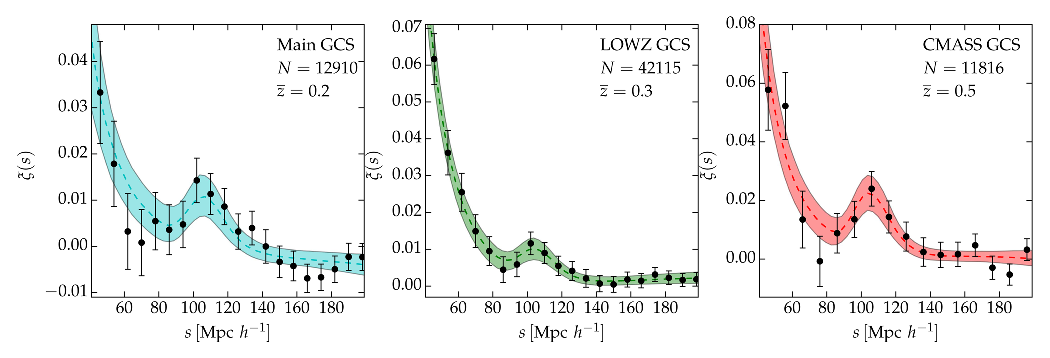
\includegraphics[width=.95 \textwidth]{Pictures/10/2pcf.eps}
    \caption{Funzione di correlazione a due punti (2PCF) nello spazio dei redshift $s$ rispettivamente per i cataloghi: Main-GCS, LOWZ-CGS, CMASS-CGS a reshift medio crescente. L'area shaded è la distribuzione a posteriori derivante dall'analisi MCMC. (From Measuring the distance–redshift relation with the baryon acoustic oscillations of galaxy clusters 2016).}\label{fig10:2pcf}
\end{figure}

\subsection{Bias osservativo}
Gli ammassi di galassie vengono assunti come buoni traccianti della distribuzione della materia a meno di un fattore di bias. In precedenza è stato introdotto come una quantità lineare: $\delta N_g / N_g = b\;  \delta \rho/ \rho$. È chiaro che, per come è stata introdotta, la funzione di correlazione scala come: $b^2$. Al giorno d'oggi si utilizzano modelli non lineari, in cui il bias non dipende semplicemente dalla massa dell'alone host e del redshift (quindi dalla cosmologia). Attraverso il modello dei picchi e del collasso sferico è possibile rendere esplicite queste dipendenze:
\begin{equation}
    b=b(M_{halo}, z) \simeq 1 + \frac{1}{\delta_c} \left(\frac{\delta_c^2}{\sigma_M^2\delta_+^2(z)}-1\right)
\end{equation}
confermate anche da simulazioni N-body e perfezionate da modelli di collasso ellissoidale. Dal momento che $\sigma_M$ decresce con $M$, $b$ è una funzione crescente di $M$; ossia oggetti più massicci tendono ad essere più clusterati (cfr. discorso delle Alpi, teoria dei picchi). Inoltre, il fattore di crescita diminuisce all'aumentare di $z$: i cluster a $z=2$ sono più clusterati di quelli a $z=0$ (sono sovradensità più estreme rispetto al valore medio del campo di densità). La $\xi$ degli ammassi ($r_0^{cluster} \sim 15\div 25$ Mpc/h a $z=0$) è più grande di quella delle galassie ($r_0^{gal} \sim 5$ Mpc/h a $z=0$). Queste sono sporcate dalla microfisica, misurando il clustering degli aloni è possibile porre constraints sulla: cosmologia conoscendo la loro massa, massa assumendo una cosmologia.

Per ragionamenti analoghi, le galassie early type sono più clusterate rispetto alle late type a parità di $z$ e questo è confermato da dati osservativi. 


\subsection{Moti peculiari}
Come già discusso, il redshift non è un buon indicatore della distanza. Questo è dovuto al fatto che le galassie possono avere una velocità peculiare $v_{pec}$ che le dissocia dal flusso di Hubble (e.g. Andromeda rispetto a noi):
$$
v = H(z)d + v_{pec}
$$
questa quantità non è sempre stimabile. L'effetto ha come conseguenza che un oggetto sferico nello spazio reale appare distorto nello spazio dei redshift (Fig. \ref{fig10:bella}). Questo tipo di distorsione è detto \textit{finger of God}. I grandi flussi di materia che collassano verso il centro sono moti \textit{bulk} e anch'essi portano a distorsioni. Si può dimostrare che $\xi(s)$ nello spazio dei redshift è in generale più piatta di $\xi (r)$ nello spazio fisico a piccoli $r$.

\begin{figure}[H]
    \subfloat[]{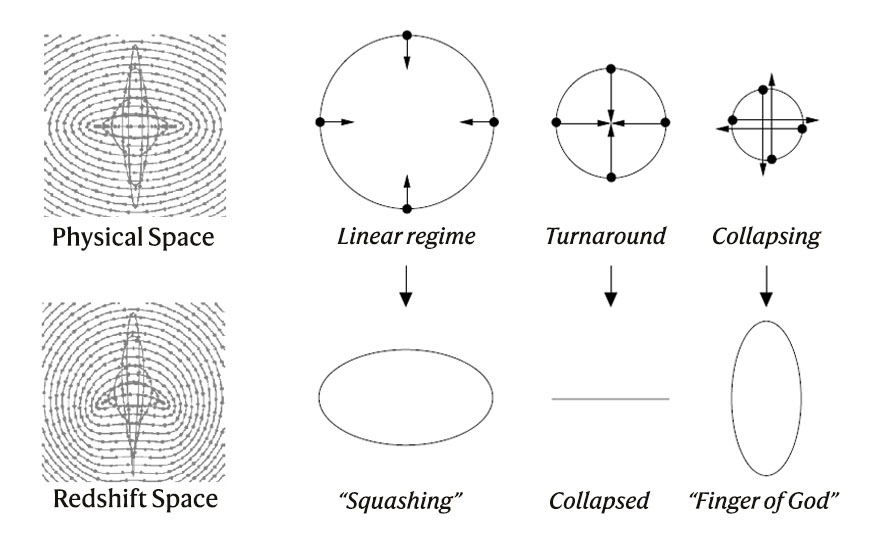
\includegraphics[width=.66\textwidth]{Pictures/10/fog.jpg}}$\;\;$
    \subfloat[]{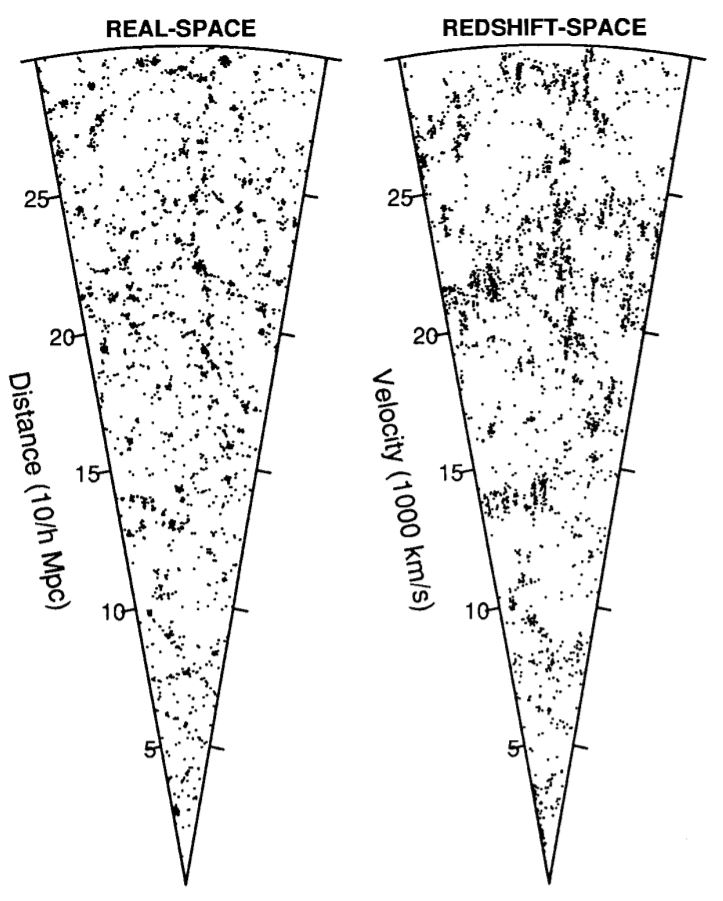
\includegraphics[width=.295\textwidth]{Pictures/10/fogsim.jpg}}
    \caption{(a) Effetto delle velocità peculiari nello spazio dei redshift. L'osservatore è posto in basso. Nell'immagine in alto a sinistra i punti rappresentano diverse galassie: quelli connessi sono galassie che distano in modo uguale dal centro di una sovradensità sferica (ammasso) nello spazio reale. A grande distanza le galassie cadono nel cluster: quelle più vicine a noi appaiono (spazio dei redshift) più distanti. Avvicinandoci alla regione interna virializzata, le velocità di dispersione aumentano e nello spazio dei redshift si forma il \textit{finger of God}.  , $v_{pec} <0$ (From: hneider Astronomy and Cosm CITAAAAS); (b) Fetta di universo simulato nello spazio reale e in quello dei redshift (From: Patron - \textit{The Bull's-Eye Effect: Are Galaxy Walls Observationally Enhanced? CITAAA.}} \label{fig10:bella} 
\end{figure}


Per ovviare a questo problema si può ricorrere alla \textbf{funzione di correlazione proiettata} lungo la linea di vista (è simile a quella angolare). Si assume che il redshift sia una misura esatta della distanza, che viene scomposta in due contributi, perpendicolare e parallelo alla linea di vista: $s^2 =  r_\perp^2 + \pi^2$. È il termine $\pi$ lungo la linea di vista che crea problemi, pertanto si integra su questa dimensione:
\begin{equation}
    W_{proj}(r_\perp ):=\int_0^\infty \xi(r_\perp, \pi)\d{\pi}=2\int_{r_\perp}^\infty\frac{\xi(s)\;\d{s}}{\sqrt{s^2-r_\perp ^2}} 
\end{equation}
dove $1+\xi(r_\perp , \pi)= DD/RR$. Proiettando si perde un po' di informazione, ma rimane soltanto quella pulita.

\vspace{1em}
Alternativamente, si può sfruttare la distorsione come informazione cosmologica. La velocità peculiare è dovuta al fatto che la materia non è distribuita in modo uniforme. Questo è un modo potente per testare la relatività generale nel tempo. Inizialmente si calcola la $W_{proj}$. Se la funzione di correlazione fosse isotropica, nel piano $(r_\perp,\pi)$ si avrebbero dei cerchi perfetti con raggio crescente al diminuire di $W$. Si assume che questa sia la funzione di correlazione nello spazio reale. La componente lungo la linea di vista si osserva invece distorta: schiacciata su grandi scale e \textit{finger of god} su piccole scale (Fig. ). Il primo è un effetto giustificabile e quantificabile dalla teoria lineare:
\begin{equation}
    \xi(s)=\xi(r)\left(1+\frac{2}{3}f+\frac{1}{5}f\right);\qquad f=\frac{\d{\ln \delta_+}}{\d{\ln a}}\simeq \Omega_M^{0.55}+...
\end{equation}
In questo modo è possibile misurare $\Omega_M$ o, meglio ancora, a diversi redshift, verificare la validità della relatività generale. Questo è uno dei test che farà Euclid. Prima questo era rumore, ora è oro. In realtà per le galassie, $f\to f/b$.
\begin{figure}[H]
    \centering
    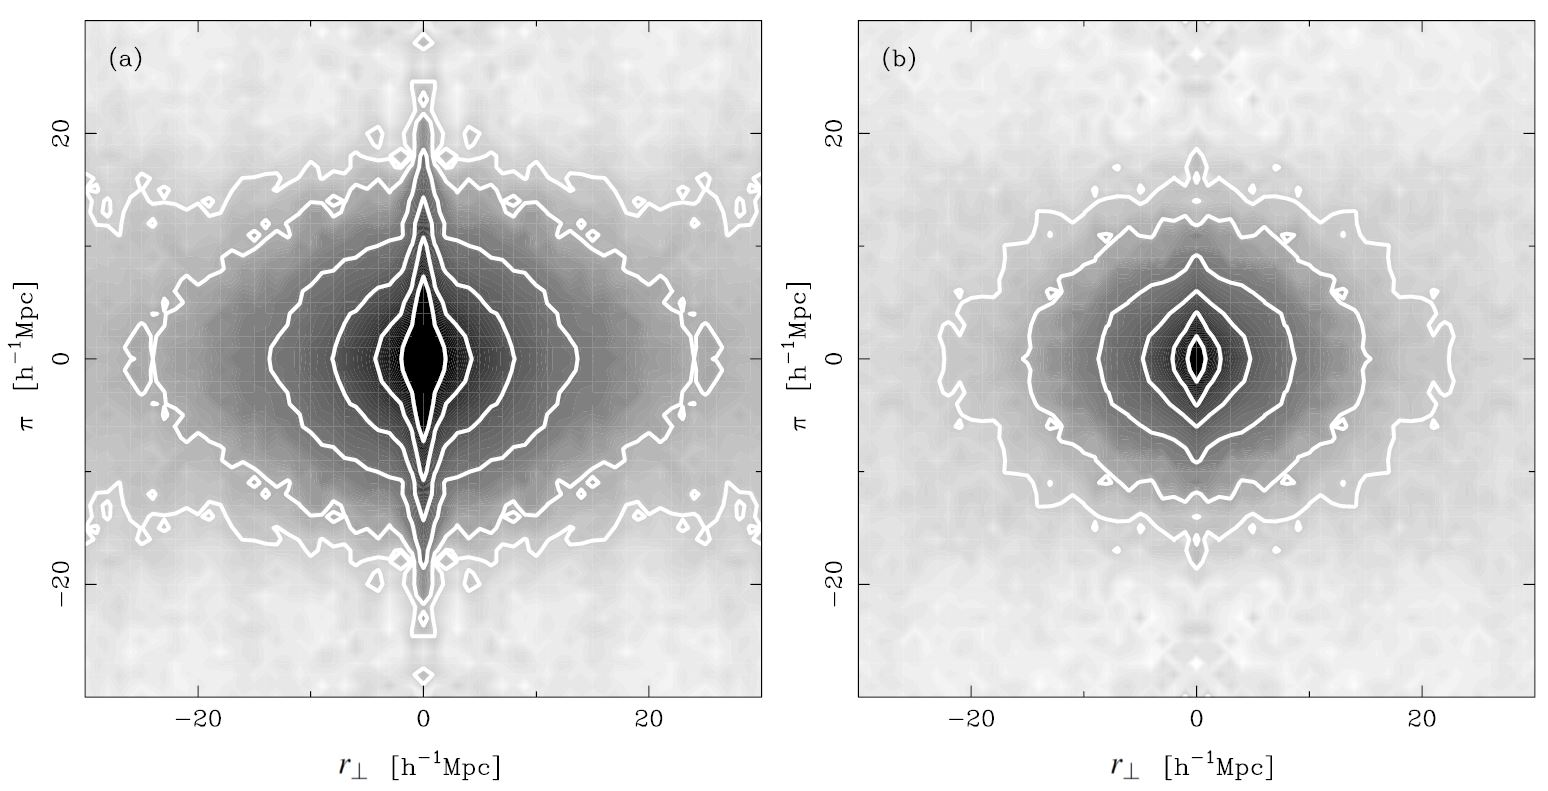
\includegraphics[width=.75 \textwidth]{Pictures/10/apforse.jpg}
    \caption{Funzioni di correlazione proiettate per: galassie quiescienti (sinistra), galassie starforming (destra). Come mai differiscono? Io forse lo so, ma non ve lo dico! (From: The 2dF Galaxy Redshift Survey: galaxy clustering per spectral type CITAAA)}
\end{figure}

\vspace{1em}
Infine, un altro modo di sfruttare questa informazione è tramite il test di \textbf{Alcock-Paczynski}. Per convertire quantità angolari e distanze in coordinate cartesiane bisogna assumere una cosmologia. Quindi il risultato della funzione di correlazione con i metodi visti in precedenza dipende anche dalla cosmologia. In questo caso si fa la procedura opposta: dopo aver modellato via tutte le distorsioni dinamiche possibili (il finger of god è il più difficile), si cerca l'unica cosmologia che restituisce $\xi (r)$ in cerchi perfetti. Questo può essere applicato su tutti gli oggetti di forma nota, e.g. sui vuoti assumendo che siano perfettamente sferici.  % Clustering
\chapterimage{/11/head.jpg} % Chapter heading image
\chapter{Cosmic Microwave Background}\label{11:ch}
Attualmente, la fonte principale di informazione cosmologica è la radiazione cosmica di fondo. È un ``bagno termico di fotoni'' osservabile da qualsiasi direzione e legato al fenomeno dell'ultimo scattering dovuto alla ricombinazione dell'idrogeno ($z\approx 1100$). La scoperta da parte di Arno Penzias e Robert Wilson è stata serendipitosa, ma la radiazione era prevista teoricamente dai modelli di nucleosintesi primordiale (ai tempi si stimava $T_0\simeq 5$K). La scoperta della CMB (metà anni `60) è stata definitiva per l'abbandono del modello stazionario, che non prevede un fenomeno di creazione di tali fotoni spiegabile semplicemente. 

La CMB è il ``corpo nero più perfetto misurato in natura'', la sua temperatura è diminuita con l'espansione dell'universo ($\sim 3000 \to 2.73$ K), ma la distribuzione è rimasta quella di un corpo nero (conservazione dei fotoni). 

Oltre a questo, si è cercato di costruire strumenti sempre più sensibili per osservare piccole fluttuazioni nella distribuzione di temperatura. Inizialmente venne osservato solo il termine di dipolo dovuto al moto relativo tra noi e il sistema di riferimento comovente, rispetto al quale la CMB dovrebbe essere isotropa (rotazione terrestre, del Sole nella Galassia, moto della Galassia). Negli anni `90 il satellite COBE ha studiato le prime fluttuazioni ccon una risoluzione di $\sim 7$ gradi. 

Il problema dell'orizzonte si nota principalmente nella CMB. Si osservano regioni di cielo con temperatura quasi uniforme su scale che ai tempi non potevano essere in connessione causale. Come già discusso, il problema è stato brillantemente risolto con il modello inflazionario. 

\vspace{1em}
Osservativamente si misura la quantità: $\frac{\delta T }{T} (\theta, \phi)=\frac{T(\theta,\phi) - \overline{T}}{\overline{T}}$ e si costruiscono mappe che coprono tutto cielo. È una quantità bidimensionale e per studiare meglio le sue caratteristiche si scompone in \textit{armoniche sferiche}. Non conviene utilizzare le trasformate di Fourier come si è fatto col campo di densità perché sono legate a quantità cartesiane. Normalmente si studiano aree estese nel cielo, in caso contrario si può sempre ricorrere all'equivalente dello spettro di potenza bidimensionale. In generale si utilizza la seguente convenzione:
\begin{equation}
    \delta_T (\theta, \phi) = \sum_{l=0}^\infty \sum_{m=-l}^{l}a_{lm}Y_{lm} (\theta, \phi); \qquad Y_{lm} (\theta, \phi):= \sqrt{\frac{2l+1}{4\pi}\frac{(l-m)!}{(l+m)!}P_l^m (\cos\theta)e^{i\phi}}
\end{equation}
dove $Y_{lm}(\theta, \phi)$ è un'armonica sferica e $P_l^m$ è il polinomio di Legendre di indici $l$ e $m$ (il primo legato a un angolo sotteso, il secondo a una direzione). L'indice $l$ assume valori tra $0$ e $+\infty$ ed è legato all'inverso dell'angolo $\theta$:
\begin{itemize}
    \item $l=0$: termine di monopolo, $\theta=360^\circ $;
    \item $l=1$: termine di dipolo, $\theta=180^\circ $;
    \item $l=2$: termine di quadrupolo, $\theta=90^\circ $;
    \item $l \gg 3$: $\theta\approx 180^\circ /l$.
\end{itemize}

Analogamente allo spettro di potenza per il campo di densità: $\mathcal{P}(k)\propto \langle|\delta_k^2| \rangle $ (mediato su tutti i $k_x$, $k_y$ e $k_z$ corrispondenti a un modulo $k$), si utilizza lo \textbf{spettro di potenza angolare}: $\mathcal{C}(l) =  \langle|a_{lm}^2| \rangle$ (mediato su tutti gli $a_{lm}$ che condividono lo stesso $l$):
\begin{equation}
    \mathcal{C}(l)=\frac{1}{2l+1}\sum_{m=-l}^l a_{lm}^2
\end{equation}
che misura quanto è importante la fluttuazione di temperatura su una data scala. Come nel caso della densità, anche $\mathcal{C}(l)$ non è una vera potenza, ma una densità di potenza. Non va confuso con lo spettro energetico, che è la plankiana!

\section{Anisotropie}
Ci sono tre meccanismi principali che causano fluttuazioni di temperatura nell'universo primordiale:
\begin{enumerate}
    \item \textbf{Gravità}: un fotone che parte in una buca di potenziale perderà eneria per uscire e verrà redshiftato, il contrario avviene per i fotoni che partono dalle creste (\textit{redshift gravitazionale});
    \item \textbf{Densità}: avendo assunto fluttuazioni di tipo adiabatico, le sovradensità corrispondono a zone più calde e le sottodensità a zone più fredde: questo meccanismo agisce in modo opposto alla gravità;
    \item \textbf{Campo di velocità}: una componente di velocità lungo la linea di vista può cambiare la temperatura osservata.
\end{enumerate}
In reatà sono tutti legati al campo di densità. Le anisotropie vengono divise in due grandi categorie:
\begin{itemize}
    \item \textbf{Primarie}: originate al momento del last scattering;
    \item \textbf{Secondarie}: si creano lungo il viaggio del fotone dal last scattering fino a noi (SZ, lensing, ...)
\end{itemize}

\subsection{Termine di dipolo}
Il termine di monopolo rappresenta matematicamente la media della quantità che si sta trasformando: la media di $\delta T/T$ è $0$ per definizione. Anche il termine di dipolo, il primo osservato storicamente, non è interessante da un punto di vista cosmologico. Essenzialmente è dovuto al moto della Terra rispetto al sistema di riferimento solidale alla CMB. Gli effetti che lo caratterizzano sono principalmente due:
\begin{enumerate}
    \item Vengono catturati più fotoni nella direzione del moto: $\delta T \propto \left(1+\frac{v }{c}\cos\theta\right)$;
    \item Aberrazione relativistica dell'angolo: $\delta F \propto \delta\Omega^{-1} \propto  \left(1+\frac{v }{c}\cos\theta\right)^2$.
\end{enumerate}
Overall, si ha che l'intensità del corpo nero riscala come $\left(1+\frac{v }{c}\cos\theta\right)^3$ più un termine del secondo ordine, pertanto:
\begin{equation}
    T'(\theta)= T(\theta) \left(1+\frac{v}{c}\cos\theta \right)\left(1-\frac{v^2}{c^2}\right)
\end{equation}
Nel 1976 è stato misurata un'anisotropia di: $\delta T / T \simeq 1.3\cdot 10^{-3}$ totalmente ascrivibile agli effetti relativistici accennati. Questa corrisponde a una velocità relativa di $v\simeq 390$ km/s, includendo i noti movimenti della Terra rispetto alla Galassia e della Galassia rispetto al Gruppo Locale, si può inferire che il Gruppo Locale si muove con $v\approx 600$ km/s rispetto la CMB (si sta muovendo verso il grande attrattore, tra l'Hydra e il Centauro).

Tutto questo però prescinde dalla cosmologia e un'eventuale velocità cosmologica sarebbe trascuraile perché su scala molto grande ($180^\circ $). 

\subsection{Termini di quadrupolo e di ordini superiori}
Analogamente allo spettro di potenza, a valori piccoli/grandi di $l$ corrispondono scale grandi/piccole. Diventa fondamentale distinguere quindi le scale che si trovano dentro e fuori dall'orizzonte al momento dell'ultimo scattering (corrispondenti a $l_H$).

\subsubsection{Scale $l<l_H$ ed effetto Sachs-Wolfe}
Fuori dall'orizzonte agisce solo la gravità. Il campo di velocità è trascurabile perché la velocità è sempre sottodominante rispetto alla densità essendo più lineare. Rimangono quindi solo i primi due meccanismi:
\begin{itemize}
    \item \textbf{Gravità}: $T\propto v^2 \propto \phi \quad\rightarrow\quad \frac{\delta T }{T}\propto \frac{\delta \phi }{\phi} =\frac{\delta \phi }{c^2}$
    \item \textbf{Densità}: $\frac{\delta T }{T} \propto - \frac{\delta a}{a} = -\frac{2}{3}\frac{\delta t }{t} = -\frac{2}{3}\frac{\delta \phi }{c^2}$
\end{itemize} 
Overall, si ha la seguente relazione, nota anche come \textbf{effetto Sachs-Wolfe}:
\begin{equation}
    \frac{\delta T}{T}\propto \frac{1}{3}\frac{\delta\phi}{c^2}
\end{equation}
Questo significa che se un fotone parte da una buca di potenziale, verrà redshiftato. Regioni di sovradensità corrispondono a macchie fredde. L'inflazione prevede fluttuazioni del potenziale con un andamento piatto $\mathcal{P}(k)\propto k^{\approx 1}$, quindi ci si aspetta uno spettro angolare del tipo $\mathcal{C}(l)\propto l^{n-1}\propto l^0$ per $l<l_H$.

\subsubsection{Scale $l>l_H$ e oscillazioni acustiche}
Su scale più piccole della scala dell'orizzonte, come più volte sottolineato, la microfisica non è più trascurabile. Vi è un periodo in cui i barioni e fotoni accoppiati sguazzano nelle buche di potenziale generate dalla materia oscura già disaccoppiata. Il signor barione vorrebbe cascarci dentro, mentre la pressione di radiazione lo spinge fuori. Il massimo della gravità corrisponde alla massimo della compressione e a una velocità della particella nulla, mentre i minimi della gravità corrispondono ai massimi della rarefazione e velocità nulle (Fig. \ref{fig11:osc}a). Modellandolo come oscillatore armonico, vi è uno sfasamento di $\pi/2$ tra il massimo della gravità e il massimo della velocità. Queste due quantità avranno un andamento del tipo $\sin\theta$ e $\cos\theta$ reciprocamente. Pertanto le oscillazioni complessive in temperatura andranno come $A^2(\sin^2\theta+\cos^2\theta)=A^2$ indipendentemente dall'angolo $\theta$. Lo spettro angolare risulta quindi costante anche per $l>l_H$, ma con una diversa normalizzazione.

\vspace{1em}
Quanto detto è valido fino al momento del disaccoppiamento, qua assunto avvenire istantaneamente. I barioni, improvvisamente liberi, si trovano in diverse posizioni delle buche di potenziale che corrispondono a un $l$ e quindi $\theta$ diversi (multipli delle stesse armoniche si troveranno nella stessa posizione). In questo discorso non si è ancora considerato il contributo della gravità del barione che non più trascurabile. Questa approfondisce ulteriormente la buca di potenziale: l'oscillazione rimane sfasata di $\pi/2$, ma le due ampiezze non sono più uguali (Fig. \ref{fig11:osc}b). L'oscillazione quindi non avviene più attorno allo $0$,ma attorno a un livello dipendente dal numero di barioni. Per  lo stesso motivo si instaura una disomogeneità nei picchi. Sommati in quadratura, i picchi pari (che corripondono ai momenti di massima rarefazione) sono più bassi dei picchi dispari (che corrispondono ai momenti di massima compressione). 
\begin{definition}
    La differenza di altezza tra picchi pari e dispari è una misura diretta del numero di barioni nell'universo (Fig. \ref{fig11:cttmodelb}).
\end{definition}

\begin{figure}[H]
    \centering
    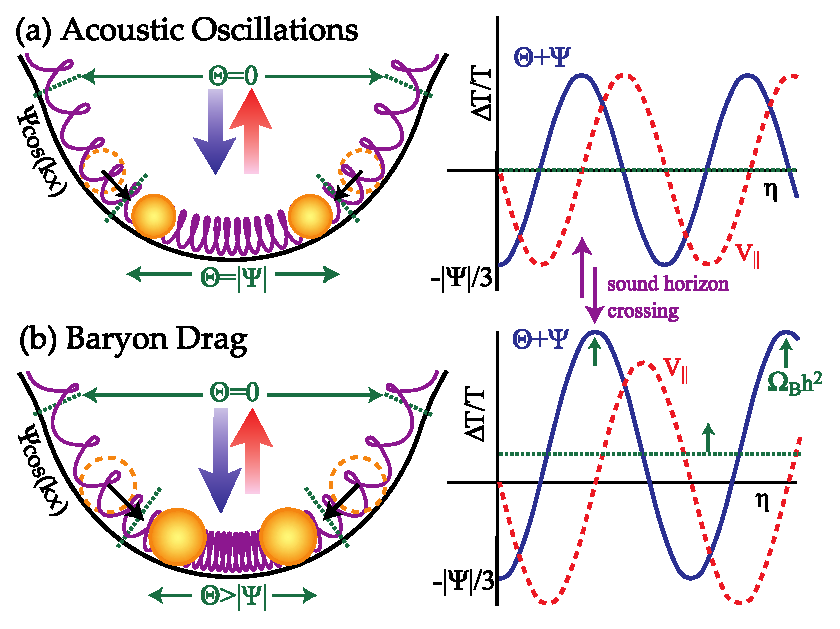
\includegraphics[width=.75 \textwidth]{Pictures/11/OscDrag.eps}
    \caption{(a) Oscillazioni acustiche tra $-\pi/2 <kx <\pi/2$. Le molle e le palline rappresentano rispettivamente pressione di radiazione e gravità. L'ampiezza delle oscillazioni vale $|\Psi|/3$ dove $\Psi$ è il potenziale newtoniano. Il blueshift dovuto alla pressione del fluido e il redshift dovuto alla gravità si bilanciano. (b)   (From: https://arxiv.org/abs/astro-ph/9604166 CITAAA)}\label{fig11:osc}
\end{figure}

\begin{figure}[H]
    \centering
    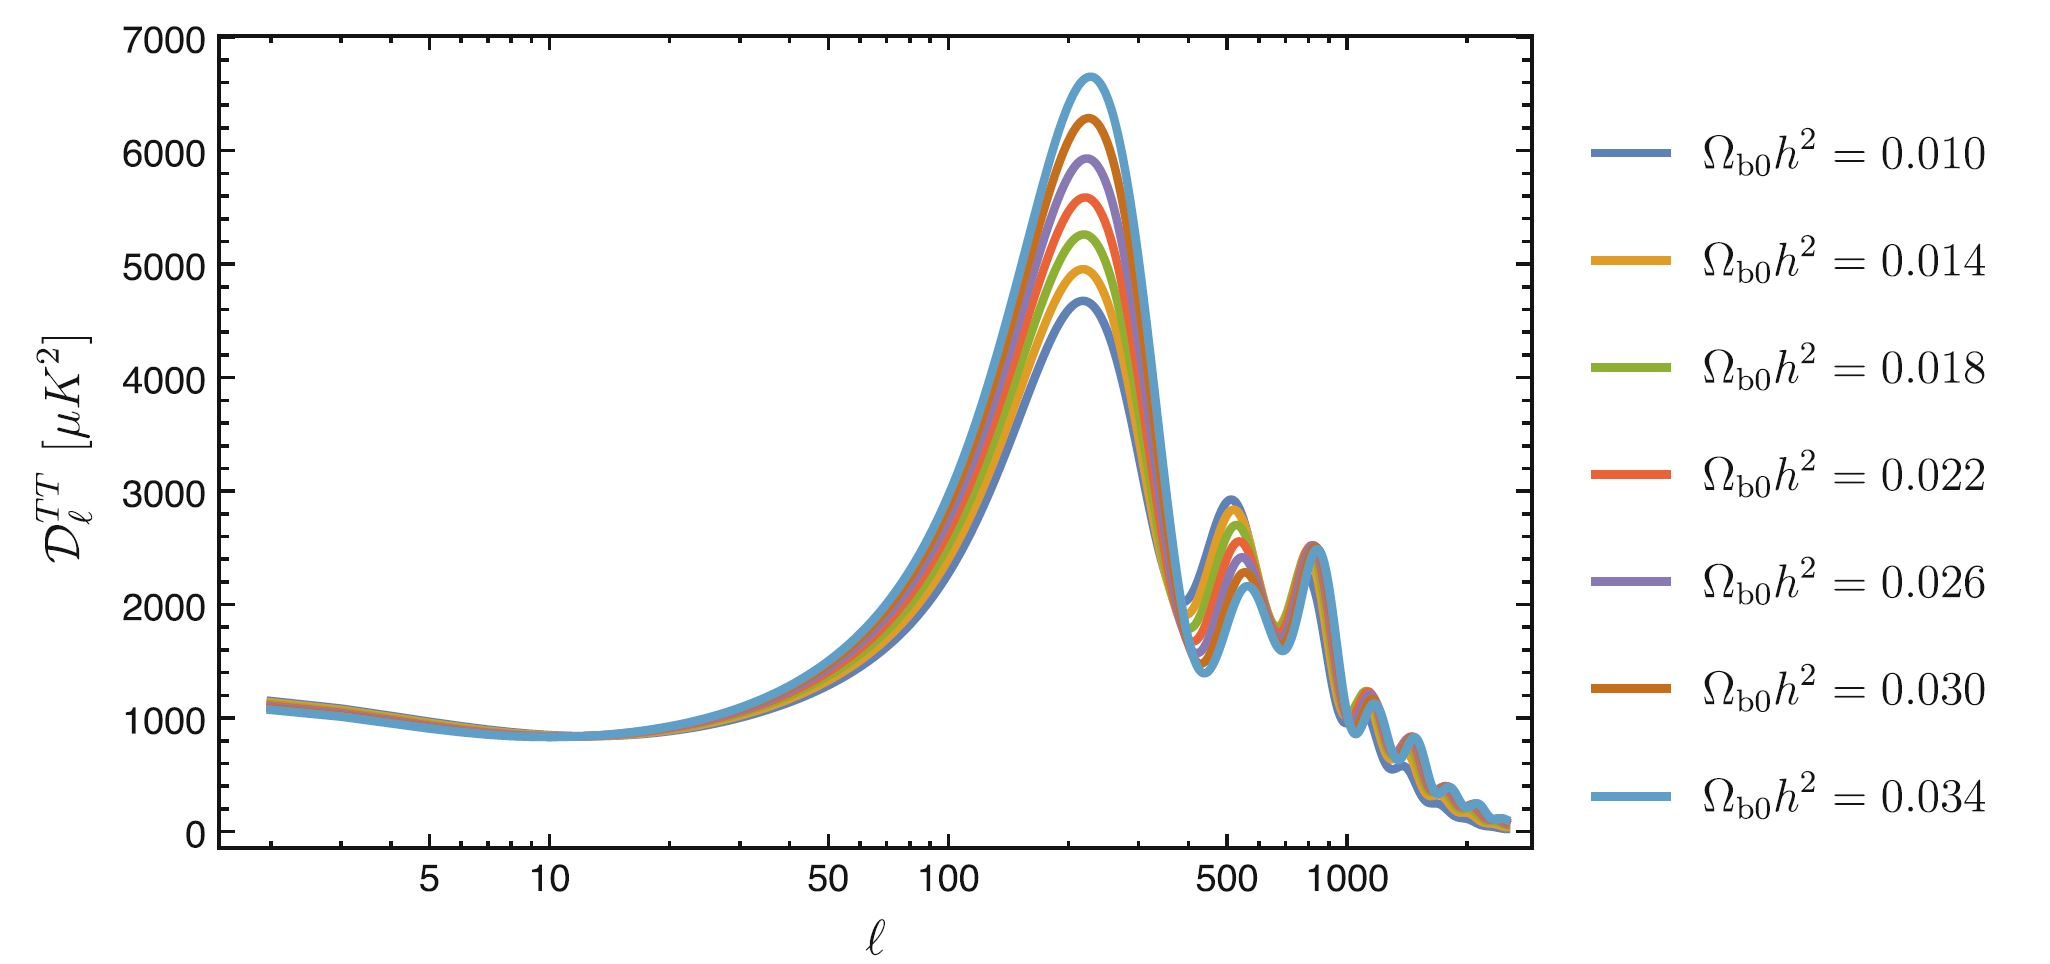
\includegraphics[width=.8 \textwidth]{Pictures/11/angspecmodel.jpg}
    \caption{Spettro angolare delle futtuazioni in temperatura modellato al variare del parametro di densità dei barioni. (FONTE Piattella CITAAAA) }\label{fig11:cttmodelb}
\end{figure}

Il primo picco è la prima scala di massima compressione dentro l'orizzonte, è quindi legata alla scala dell'orizzonte al momento dell'ultimo scattering. Le oscillazioni acustiche non possono avvenire per $l\to \infty$ perché il Sig. Silk ci ha già detto che esiste una scala di dissipazione per l'oscillazione dei barioni. Il taglio ha un andamento del tipo $l^{-4}$. Osservativamente si ha lo spettro mostrato in Figura \label{fig11:cttobs}.




\section{Anisotropie Secondarie}
Dalla superficie dell'ultimo scattering fino a noi i fotoni possono andare incontro a interazioni che modificano lo spettro angolare delle fluttuazioni primitivo. Nella \href{http://background.uchicago.edu/~whu/intermediate/intermediate.html}{pagina web del Professor Wayne Hu} è possibile trovare animazioni che rendono più chiari i concetti che verranno discussi.

\subsection{Effetto Sachs-Wolfe Integrato}
È dovuto a fluttuazioni del potenziale gravitazionale lungo la linea di vista. Viene suddiviso in tre categorie:
\begin{itemize}
    \item \textbf{Late ISW}. A livello lineare in un universo EdS la fluttuazione del potenziale gravitazionale è costante. Per universi in cui $\delta_+ \not\propto a$ (e.g, universi curvi, modelli piatti con costante cosmologica,...) si ha $\dot{\delta\phi}\neq 0$, pertanto si osservano fluttuazioni nella tempreratura dovute a questo fenomeno;
    \item \textbf{Early ISW}. L'equivalenza avviene a $z_{eq}\approx 6000$, la ricombinazione a $z_{rec}\approx 1500$. Anche se piccolo, vi è un intervallo temporale in cui una bassa, ma non nulla densità di radiazione determina un andamento: $\delta_+ \propto \gtrsim a$ generando un $\dot{\delta\phi}> 0$. Questi primi due effetti devono avvenire entro l'orizzonte al momento in cui si verificano. L'early rompe le scatole su scale leggermente a sinistra del primo picco, il late a $z\approx 1\div 2$, ossia a scale grandi ($l$ bassi) (Fig. \ref{fig11:secanisot}).
    \item \textbf{Rees-Sciama}. È dovuto alla non linearità. Se, nel tempo, la buca di potenziale / vuoto si approfondisce / livella più del dovuto il fotone subisce una predita / guadagno netto di energia. 
\end{itemize}
Questi effetti sono dovuti alla distribuzione della materia, per amplificare il segnale cosmoogico vengono osservati cross-correlando la CMB e la struttura su larga scala. 

\begin{figure}[H]
    \centering
    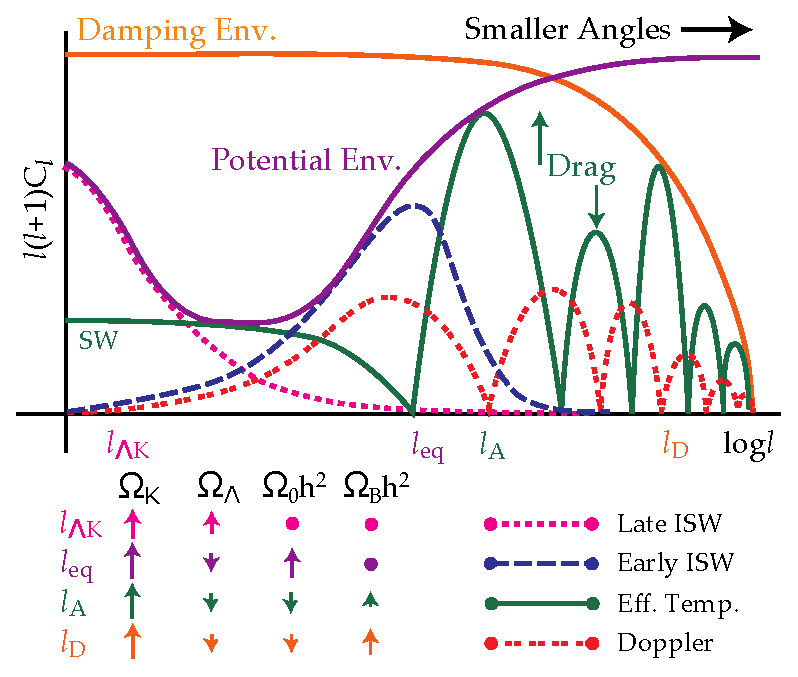
\includegraphics[width=0.75 \textwidth]{Pictures/11/secanisotropies.eps}
    \caption{Spettro delle anisotropie su scala logatitmica. L'andamento di $l_{\Lambda K}$ e di $l_{eq}$ genera il pateau di Sachs-Wolfe (SW). Il baryon drag intensifica i picchi dispari e può essere una probe per le fluttuazioni all'ultimo scattering e/o $\Omega_b h^2$.} \label{fig11:secanisot}
\end{figure}

\subsection{Lensing gravitazionale}
Anche questo dipende dalla distribuzione della materia. Non cambia le temperature dei fotoni, ma soltanto il tragitto dei fotoni. Pertanto, il lensing sfoca le mappe di temperatura. 

\subsection{Effetto Sunyaev-Zeldovich}
Il fotone può anche interagire con la materia reionizzata dai fenomeni di galaxy evolution a partire da $z\approx 5$. Essendo di bassa energia interagisce con gli elettroni caldi per effetto compton inverso. Questo fenomeno può avvenire globalmente su grandi scale e localmente negli ammassi di galassie, lobi delle radio galassie e così via\dots Naturalmente questo fenomeno può avvenire solo su scale non più grandi dell'orizzonte, generalmente $l>10$. Con il passare del tempo la densità barionica media e quella della radiazione decrescono, quindi la probabilità di avere scattering inverso sarà sempre minore. Ulteriori dettagli sono riportati in Figura \ref{fig11:sz}.



\section{Risultati osservativi}
Come già discusso, \textbf{la posizione (non il valore) del primo picco} è legata alla scala dell'orizzonte al momento dell'ultimo scattering. Il valore: $R_H(z_{LS})=a(z_{LS})\int_0^{t_{LS}}c \; \d{t} / a(t)$ può esssere in buona approssimazione calcolato per un universo EdS. Questa quantità può essere utilizzata come un righello standard. L'angolo sotteso da questo righello dipende dalla geometria (Fig. CITAAAA): $\Omega_k = 1-\Omega_{TOT}$. All'aumentare di $\Omega_k$ (universo aperto) la scala diventa più piccola e l'intero spettro shifta rigidamente verso $l$ grandi. La posizione osservata (per la prima volta con l'esperimento BOOMERanG) del primo picco, $l=220$, corrisponde esattamente a una geometria piatta.

\begin{definition}
    L'evidenza più importante della piattezza dell'universo è aver osservato un angolo sotteso dal raggio dell'orizzonte al momento dell'ultimo scattering corrispondente a $l=220$ ($\theta \approx 1^\circ$), esattamente come previsto da una geometria piatta ($\Omega_{TOT}=1$). Con lo spettro di potenza della materia si osservava invece una combinazione di $\Omega_m$ e $H$ perché il momento dell'equivalenza è altamente determinato dalla quantità della materia.
\end{definition}

La \textbf{differenza di altezza tra i picchi dispari e i picchi pari} si acuisce all'aumentare di $\Omega_b$. Questa misura viene fatta per ogni coppia di picchi adiacenti, ma per effetto della diffusione si ha più segnale tra il primo e il secondo. Il fit dei dati di Plank ha restituito: $\Omega_b h^2 = 0.022$, che corrisponde a $\Omega_b =0.045$ assumendo $H_0=70$ km/s/Mpc, oppure $\Omega_b =0.049$ assumendo $H_0=67.4$ km/s/Mpc (come derivato dai dati di Plank). Entrambi consistenti col valore derivato dalla nucleosintesi. La dipendenza dalla costante di Hubble deriva dalla definizione di $\rho_{crit}$.

A \textbf{$l$ piccoli} si può misurare il livello di normalizzazione dello spettro di pontenza (nemmeno l'inflazione riesce a predirlo!), l'indice spettrale delle perturbazioni primordiali $n_s$ e l'effetto Sachs-Wolfe integrato dovuto a un'eventuale curvatura dell'universo e/o alla presenza di energia oscura (la quale sposta anche debolmente il primo picco verso sinistra). Per osservare \textbf{$l$ grandi}, quindi il regime di dissipazione, è necessario avere un'ottima sensibilità degli strumenti. Attenzione, $\mathcal{C}(l)$ si ottiene mediando su tutti gli $m$ possibili: è semplice osservare $l$ piccoli, ma si ha bassa statistica (grandi errori); è più complesso osservare $l$ grandi, ma si ha molta più statistica.

Può verificarsi anche una \textbf{soppressione della potenza ad alti multipoli}. Questo è dovuto principalmente alla profondità ottica e al redshift della reionizzazione e in secondo luogo alle onde gravitazionali. Questi fenomeni sono visibili anche studiando la polarizzazione della CMB. 

Le prime osservazioni delle fluttazioni cosmologiche, predette e richieste dai modelli di formazione delle strutture, $\delta T / T \simeq 10^{-5}$ sono state osservate da COBE nel 1992. In seguito, fu lanciato dall'Antartide l'esperimento BOOMERanG, sfruttando l'effetto dei venti per rimanere in volo diversi giorni su un'orbita più o meno circolare. Non venne fatta una mappa all sky, ma su una regione piccola di $25^\circ $ con una risoluzione e sensibilità tale da osservare la posizione del primo picco. Per la prima volta venne osservato $\Omega_0 =1$. WMAP (americano) e Plank (europeo) vennero progettati a partire dal 1992, il primo fu lanciato nel 2003, il secondo nel 2009. In realtà, alle frequenze di osservazione, non si vede nulla di cosmologico. I contributi di \textit{foreground} dovuti al sincrotrone e alla polvere termale (cit.) sono sottodominanti soltanto tra 30 e 100 GHz (Fig. \ref{fig11:cmbsporca}). Una volta mappata bene la loro distribuzione energetica è possibile modellarli e sottrarli per isolare il segnale cosmologico.

\begin{figure}[H]
    \centering
    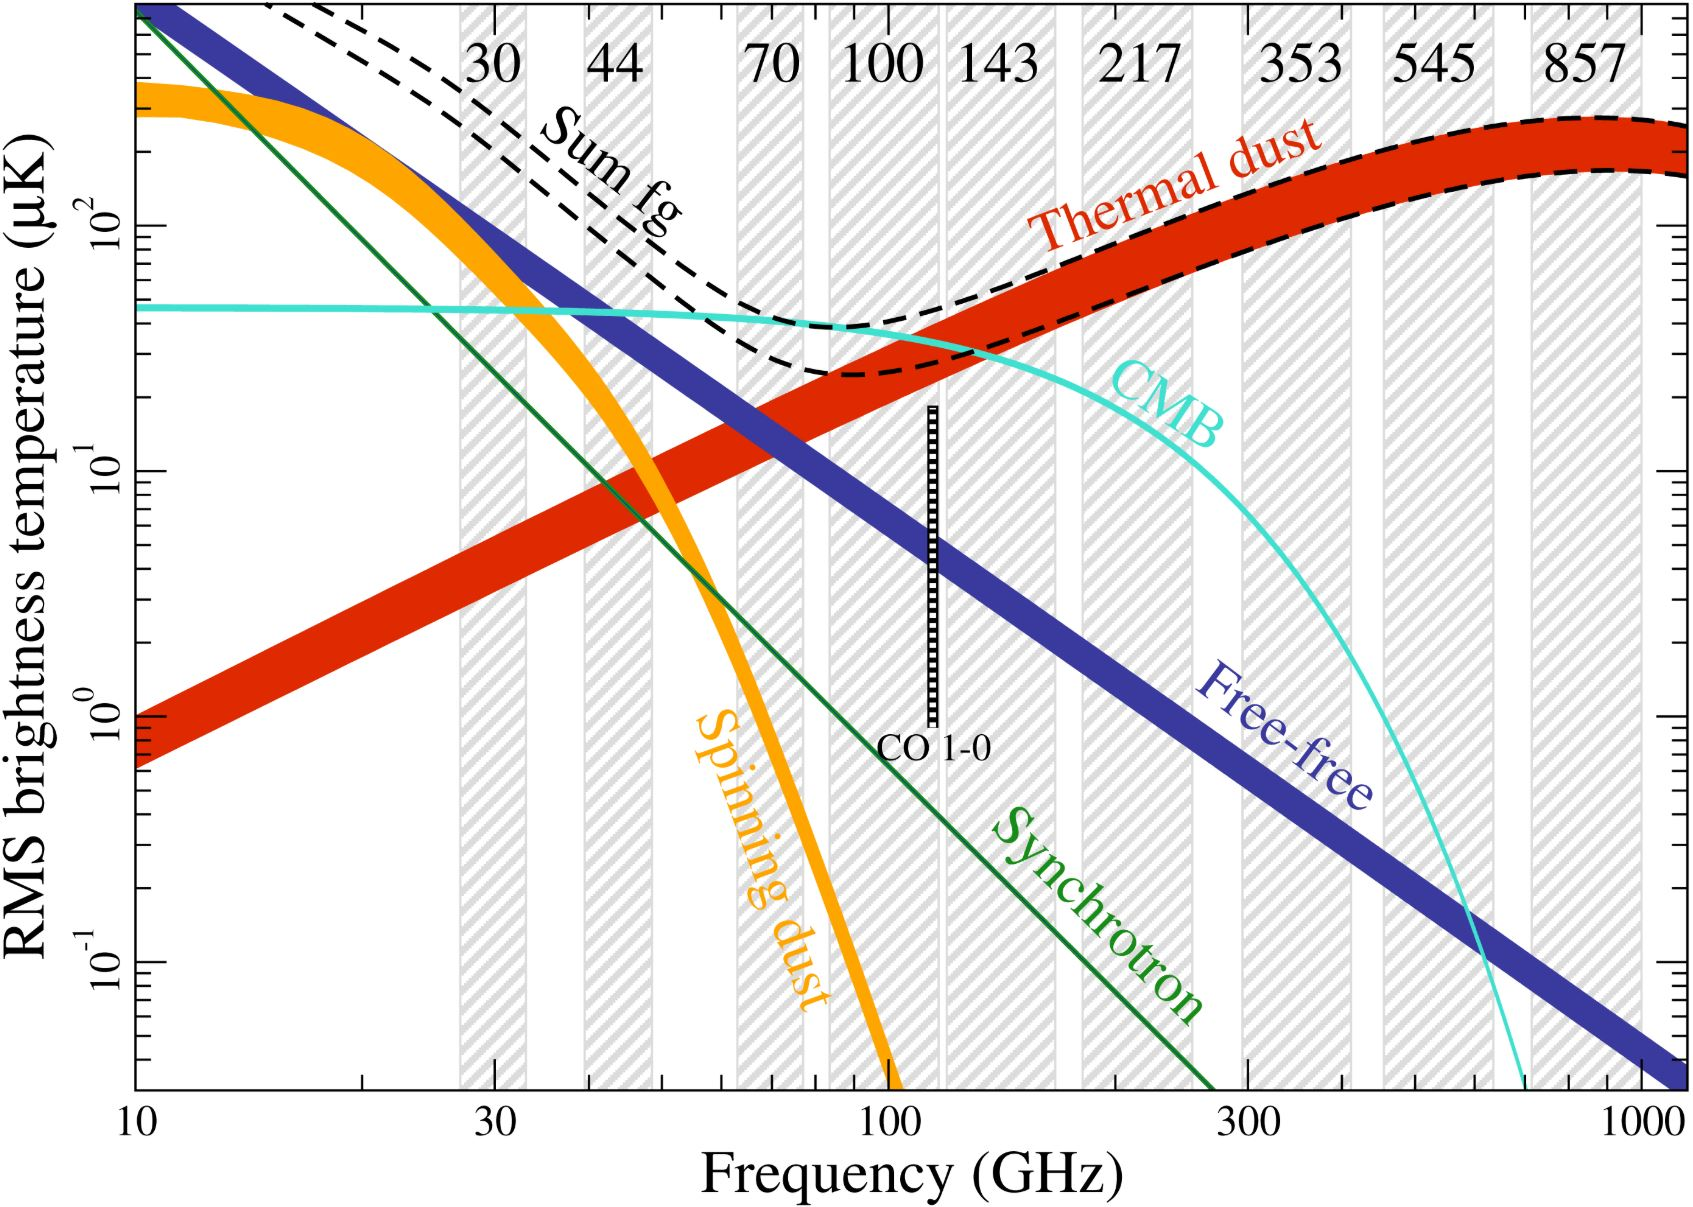
\includegraphics[width=0.65 \textwidth]{Pictures/11/falsecmb.jpg}
    \caption{Spettro angolare delle futtuazioni in temperatura teorico (linea continua) e multipoli osservati tramite la CMB (punti). Le bande shaded sono quelle utilizzate da Planck per mappare, modellare e sottrarre le componenti fastidiose per i cosmologi, ma importanti per i radioastronomi (From: ESA).}\label{fig11:cmbsporca}
\end{figure}

A questo punto la CMB si scompone in multipoli, mediando su tutti gli $m$ possibili su ogni scala corrispondente a $l$. L'ultima misura del team di Plank è riportata in Figura \ref{fig11:cttobs}. 


\begin{figure}[H]
    \centering
    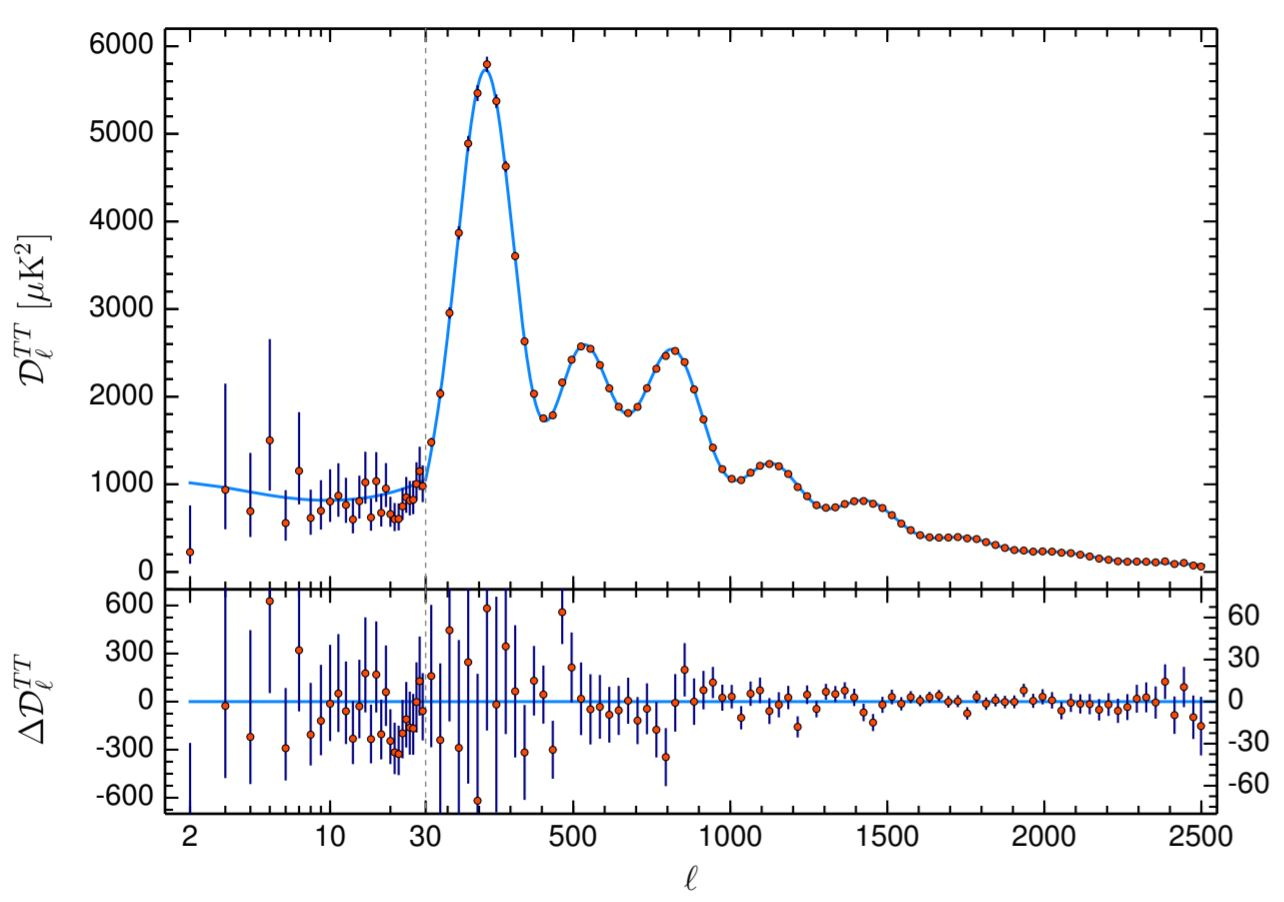
\includegraphics[width=0.72 \textwidth]{Pictures/11/angspecobs.jpg}
    \caption{Spettro angolare delle futtuazioni in temperatura teorico (linea continua) e multipoli osservati tramite la CMB (punti). Qui, $\mathcal{D}^{TT}_l:= l(l+1)\mathcal{C}_l / (2\pi)$ (From: Plank 2018 CITAAAA).  }\label{fig11:cttobs} 
\end{figure}
Chi ha l'occhio molto attento può notare qualche problemino qua e là con il modello ($l=5$, $l\approx 20$, attorno al primo picco, ...). Si parla di \textit{anomalie}. Si è arrivati più o meno ad osservare il settimo picco, $l\simeq 2500 \leftrightarrow \theta \simeq 0.07^\circ$. Notare che la scala è logaritmica per $l<30$ e lineare per $l>30$. Il fit dei dati restituisce constraints sui sei principali parametri cosmologici (numero minimo dei prarametri possibile) e quattro parametri importanti derivati:
\begin{figure}[H]
    \centering
    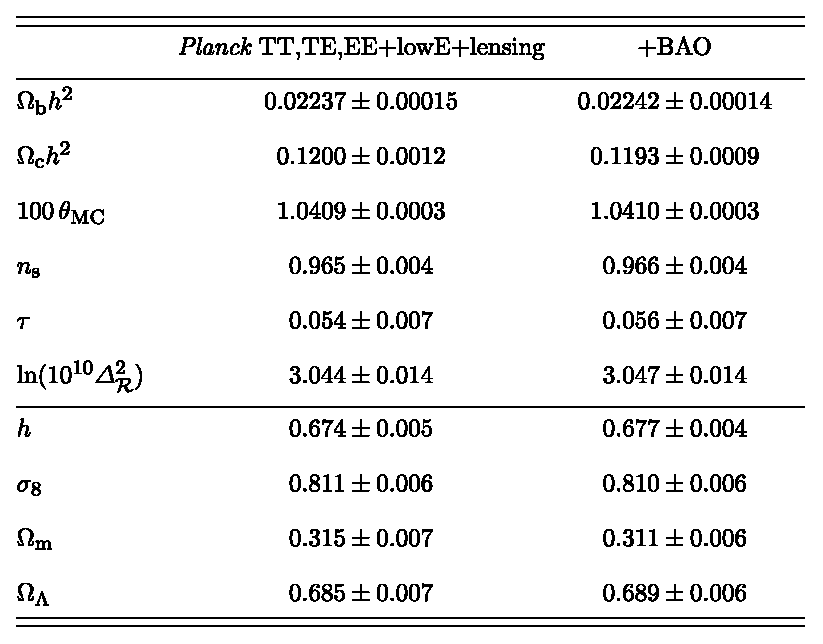
\includegraphics[width=0.65 \textwidth]{Pictures/11/planktable.eps}
\end{figure}
I sei parametri del fit sono rispettivamente: $\Omega_b h^2$, $\Omega_{DM} h^2$, 100$\times$ la scala dell'orizzonte sonoro al disaccoppiamento, indice spettrale delle perturbazioni primordiali, profondità ottica dovuta alla reionizzazione (è un segnale di disturbo) e normalizzazione dello spettro primordiale. Tra i parametri derivati vi sono: $H_0$, $\sigma_8$, $\Omega_m$ e $\Omega_\Lambda$. Inoltre con altri dati esterni, si può inferire una stima della somma delle masse dei diversi tipi di neutrini: $\sum m_\nu <0.13$ eV (ancora consistente con zero). Si può anche testare una delle ipotesi dell'inflazione: la gaussianità delle perturbazioni ($f_{NL}=0$). Si osserva una leggera e trascurabile deviazione dalla gaussianità a $z\sim 1000$, con un valore di $f_{NL}\in(-60,+60)$. Questa misura, assieme alla quantità $\d{n_s}/\d{\ln k}\in (-0.03, 0.015)$ ha comunque permesso di scartare moltissimi modelli. Infine si può studiare se le perturbazioni sono adiabatiche come è stato fino ad ora assunto (porebbero essere isoterme, di isocurvatura, ...): la deviazione di quantifica tramite la quantità $\alpha$. Planck ci assicura che $\alpha \simeq 0$ (al massimo un po' di isocurvatura). 

Una volta caratterizzati completamente gli effetti cosmologici si possono estrarre informazioni sull'effetto Sachs-Wolfe integrato correlando la CMB e la struttura a larga scala. Come ci si aspetta dal modello $\Lambda$CDM, il potenziale gravitazionale varia a redshift bassi (dark energy). Lo stesso vale per l'effetto di lensing subìto dai fotoni della CMB. 

Ad oggi ci sono due parametri che danno problemi: $H_0$ come già discusso e $\sigma_8$ (problema interno ai dati di Planck); sugli altri c'è buona convergenza con altri osservabili astrofisici. In particolare il valore di $\sigma_8$ misurato direttamente tramite la CMB è in contrasto con il valore di $\sigma_8$ che si ricava utilizzando campioni di ammassi estratti dalla CMB stessa grazie all'effetto SZ. La differenza può essere lenita dalla presenza dei neutrini.

\begin{figure}[H]
    \subfloat[]{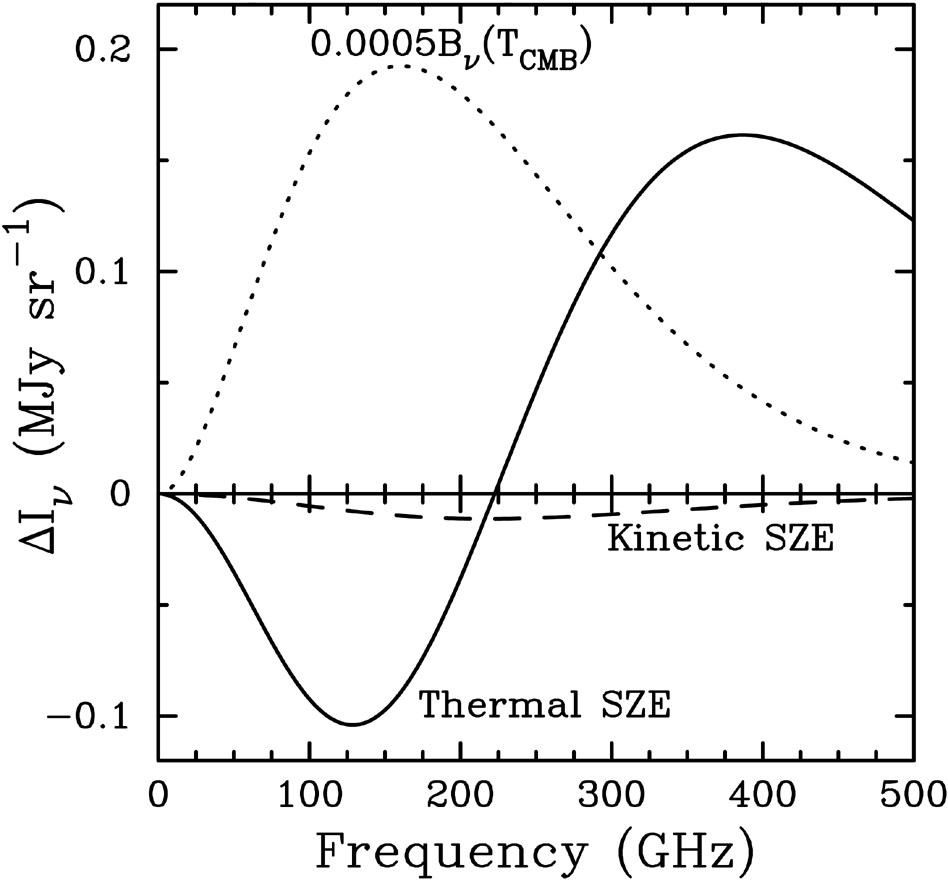
\includegraphics[width=.415\textwidth]{Pictures/11/sz.jpg}}$\;\;$
    \subfloat[]{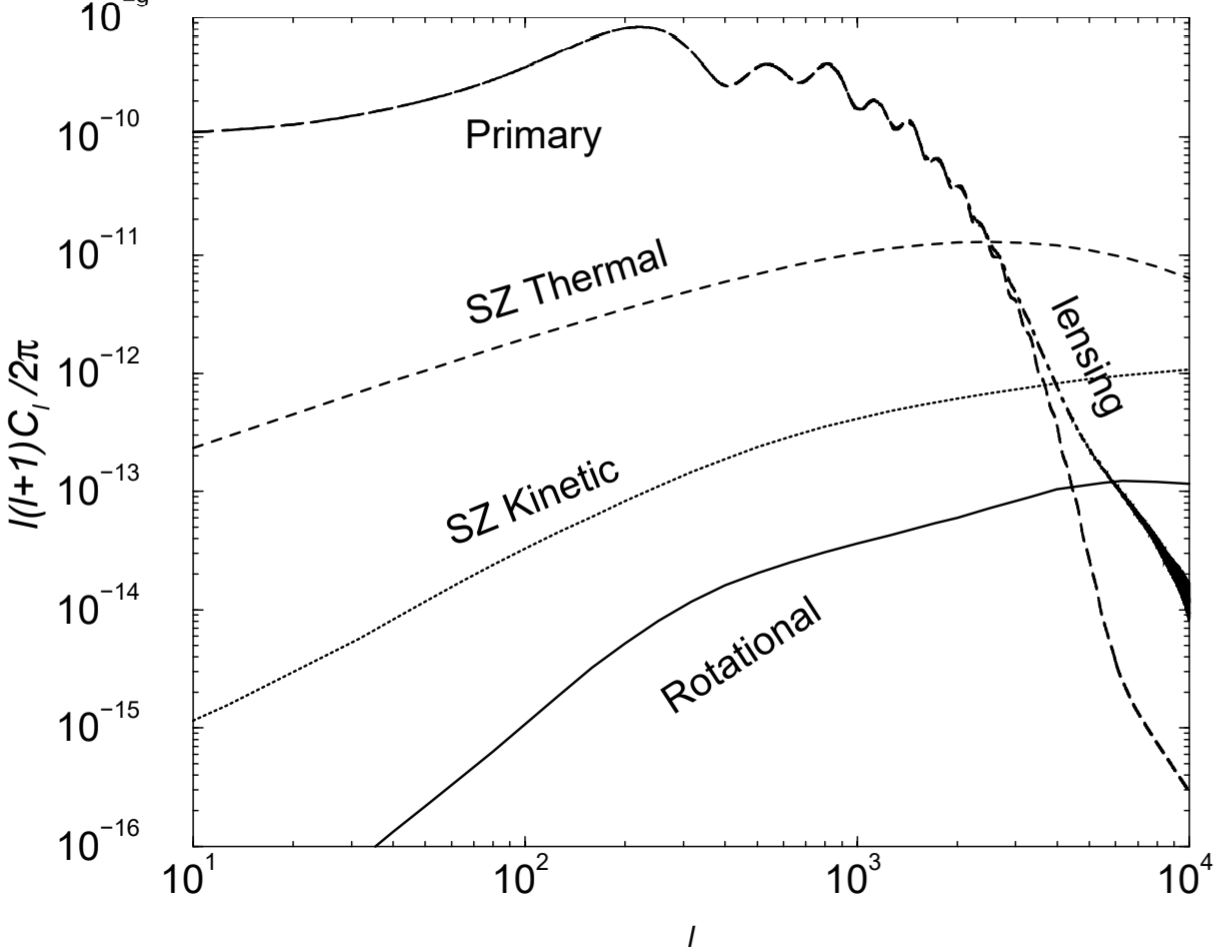
\includegraphics[width=.5\textwidth]{Pictures/11/szang.jpg}}
    \caption{(a) Risultato netto dell'effetto SZ sulla CMB. Il corpo nero della CMB è upscatterato a energie maggiori. Osservando la deformazione del corpo nero $\Delta I_\nu$ si nota che il turnover è a $\nu_t \simeq 217$ GHz.  (From: J. Carlstrom); (b) L'effetto SZ agisce su $l$ grandi ed è dovuto a tre fenomeni, di cui quello termico è il più importante (From: Kinetic Sunyaev-Zeldovich Effect from Halo Rotation)} \label{fig11:sz} 
\end{figure}


\subsection{Polarizzazione}
L'osservazione dello \textbf{spettro angolare del segnale di polarizzazione} è stata la vera rivoluzione del satellite Planck rispetto ai suoi predecessori. Ci si aspetta una polarizzazione della radiazione a causa delle proprietà dello scattering Thomson: l'onda scatterata è polarizzata perpendicolarmente al piano di incidenza. La CMB è polarizzata al 10\% a causa dello scattering degli elettroni liberi sulla superficie dell'ultimo scattering (fisicamente, si ha un segnale non nullo sulla scala di $90^\circ$ che corrisponde ad avere polarizzazione lineare). Lo spettro di polarizzazione è in fase con il campo di velocità, quindi è in antifase con lo spettro angolare e ha un valore di normalizzazione pari al 10\%. La reionizzazione introduce effetti di polarizzazione locale, che non hanno nulla di cosmologico. 

Le osservazioni di Plank hanno comfermato il modello dell'oscillatore armonico e hanno sfruttato queste informazioni per porre migliori constraints sui parametri cosmologici. La polarizzazione può essere scomposta tramite gli equivalenti dei parametri di Stokes che tengono conto della direzione di propagazione dell'onda: i modi $E$ e $B$. I primi hanno rotore nullo (traslazioni), i secondi tracciano le rotazioni. Si possono avere diversi tipi di fluttuazioni. Le fluttuazioni di densità sono scalari e generano soltanto modi $E$, quelle del campo di velocità (trascurabili, decadono  velocemente) sono di tipo vettoriale. Le onde gravitazionali sono fluttuazioni di tipo tensoriale e generano anche modi $B$. Misurando quindi i modi $B$ si possono misurare le onde gravitazionali primordiali. 

La polarizzazione $E$ è stata ben misurata, anche sfruttando la cross-correlazione tra il segnale in temperatura e il modo $E$, $TE$. A oggi, 3 gennaio 2020, non c'è alcuna evidenza di onde gravitazionali primordiali. 


\begin{figure}[H]
    \centering
    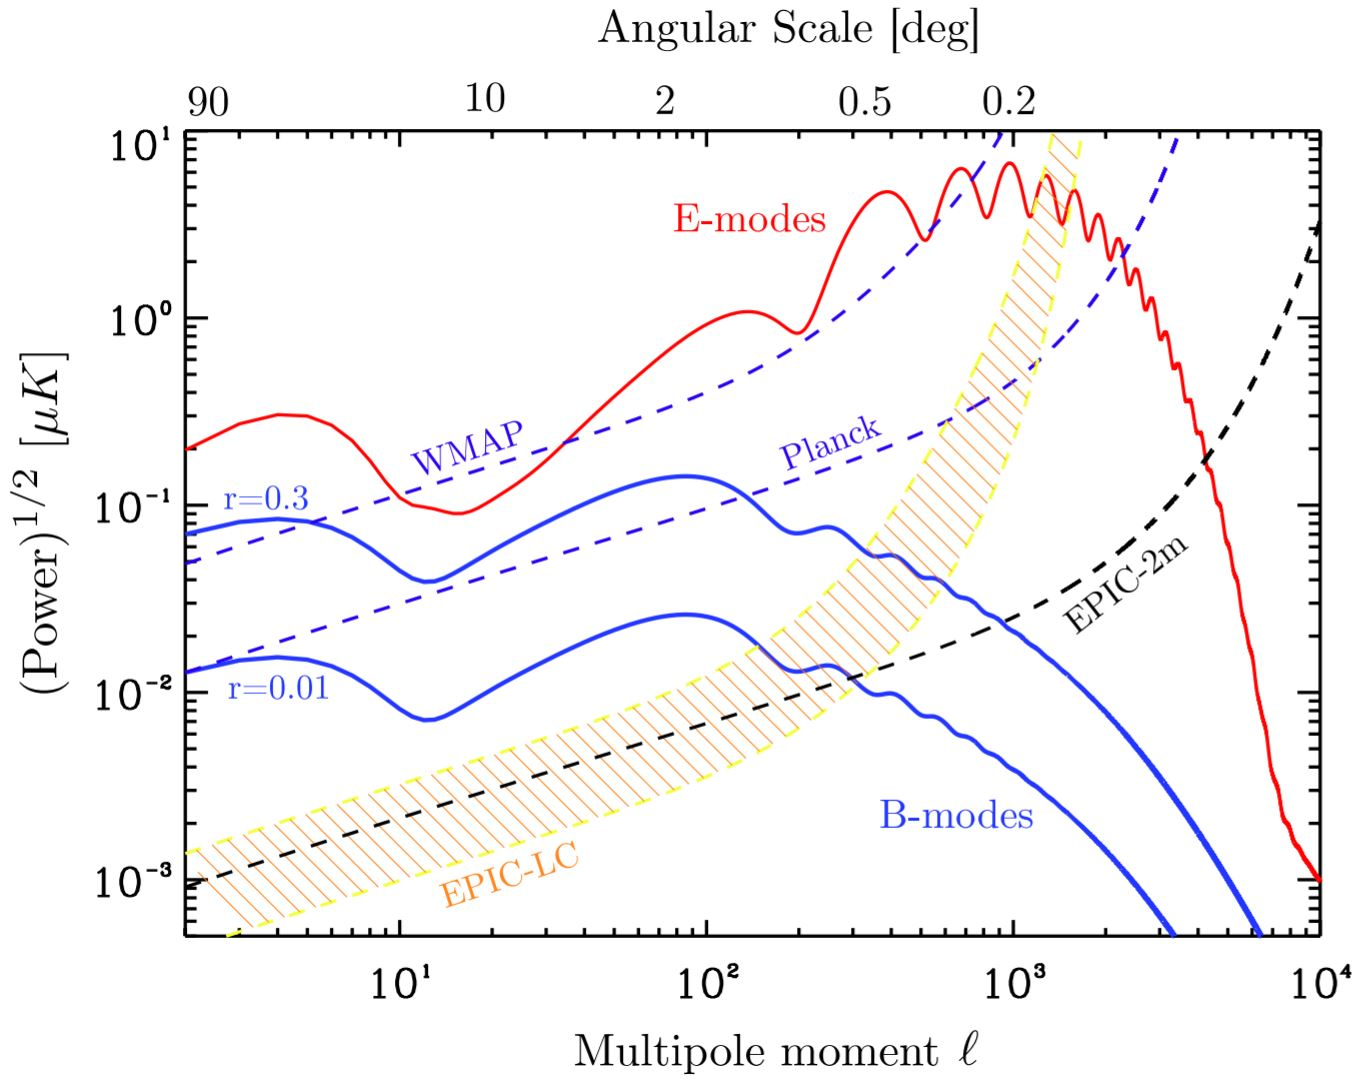
\includegraphics[width=0.7\textwidth]{Pictures/11/eb.jpg}
    \caption{Spettro di potenza per i modi $E$ e $B$. Il valore $r$ è il \textit{tensor-to-scalar ratio}. Sono mostrati i livelli di sensitivity di WMAP, Plank e quella prevista per CMBPol (EPIC-LC e EPIC-2m), non costruito (from: https://arxiv.org/abs/0811.3911).}
\end{figure}




\subsection{Oscillazioni acustiche barioniche (BAO)}
Sono una delle prove fondamentali che svolgerà Euclid. I picchi sullo spettro angolare della CMB (dovuti alle oscillazione acustiche dei barioni nelle buche di potenziale della materia oscura) lasciano un'impronta sulla distribuzione a grande scala. Osservandole, si può misurare come varia il righello standard dell'orizzonte cosmologico al variare del redshift. 

A $z$ molto alti non interessa la cosmologia, ma solo la geometria. A $z$ diversi si può tracciare l'espansione dell'universo ricavando $H(z)$, utilizzando la distanza di diametro angolare e non quella di luminosità. L'\textbf{orizzonte sonoro} (i fotoni, avendo sul groppone i fotoni hanno $v<c$) al momento dell'ultimo scattering è stato misurato da Plank e vale $s=(4.53\pm 0.06)\cdot 10^{24}$ m, ossia $\sim 150$ Mpc.
Ci si aspetta che in corrispondenza dei picchi della CMB ci siano anche piccole oscillazioni nello spettro della materia (Fig. \ref{fig11:bao}), dell'ordine del 5\%. 

Il fenomeno può essere semplificato come segue. Si consideri una singola perturbazione nell'universo primordiale: la pressione di radiazione spinge i barioni e i fotoni verso l'esterno della buca di potenziale formando una shell, l'espansione continua per $\sim 10^5$ yr. A questo punto la temperatura dell'universo è scesa a tal punto da consentire la ricombinazione dell'idrogeno. La radiazione, ora disaccoppiata, fluisce via e si omogenizza. La distribuzione di materia barionica ha quindi perso il supporto che le garantiva l'espansione e rimane in stallo su una shell di raggio $\sim 100$ Mpc. Allo stesso tempo la buca di potenziale della dark matter comincia a richiamare verso il centro della perturbazione la materia barionica. L'evoluzione dell'universo determina una crescita delle perturbazioni fattore $\sim 1000$, ma nella configurazione di equilibrio della materia dark e barionica rimane una feature legata alla dimensione della shell della materia barionica. 

La prima evidenza osservativa di BAO è ad opera di Eisenstein e collaboratori (Fig. \ref{fig11:baoobs}), che analizzando la funzione di correlazione delle galassie della SDSS hanno trovato la feature a circa $100 h^{-1}$ Mpc.

\begin{figure}[H]
    \centering
    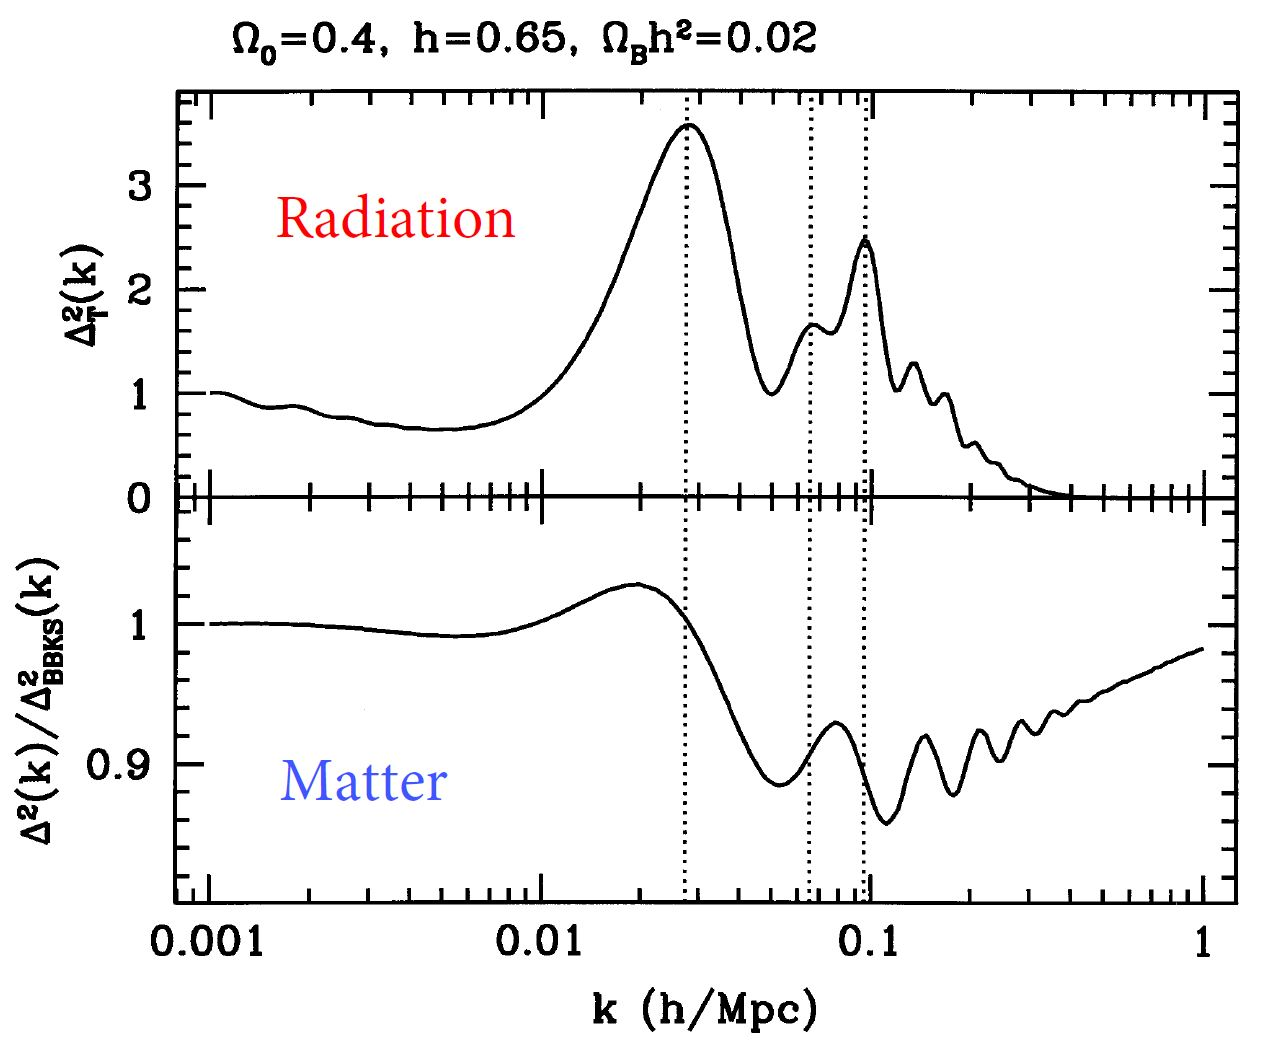
\includegraphics[width=0.7\textwidth]{Pictures/11/BAO.jpg}
    \caption{Spettro di potenza per CMB (radiazione) e LSS (materia). Non assomigliano a quelli visti perché hanno diverse normalizzazioni. (from: Baryonic signatures in large-scale structure).}\label{fig11:bao}
\end{figure}

\begin{figure}[H]
    \centering
    \includegraphics[width=0.7\textwidth]{Pictures/11/baoobs.jpg}
    \caption{Funzione di correlazione nello spazio dei redshift costruita dal campione SDSS LRG. Il bump è statisticamente significativo. (from: DETECTION OF THE BARYON ACOUSTIC PEAK IN THE LARGE-SCALE
    CORRELATION FUNCTION OF SDSS LUMINOUS RED GALAXIES
    ).}\label{fig11:baoobs}
\end{figure}

\textit{Complimenti per essere arrivati fino a qui, grazie per l'attenzione e speriamo che Euclid non cambi troppo le carte in tavola. A seguire qualche spunto per approfondire i temi trattati}.

\vspace{1em}
\begin{flushright}
LBL, 2020
\end{flushright}  % CMB

\chapterimage{/99/head.jpg} % Chapter heading image
\chapter{Dalla letteratura}\label{last:ch}

Una galleria di articoli e belle immagini per spunti di approfondimento. Ora tocca a voi...




\section{Annual Review of Astronomy and Astrophysics}
\subsection*{Ferreira - Cosmological Tests of Gravity (2019)}
\url{https://doi.org/10.1146/annurev-astro-091918-104423}

\begin{figure}[H]
    \centering
    \includegraphics[width=.75 \textwidth]{Pictures/99/ei2018-1.jpg}
\end{figure}
\begin{figure}[H]
    \centering
    \includegraphics[width=.86 \textwidth]{Pictures/99/ei2018-2.jpg}
\end{figure}
\begin{figure}[H]
    \centering
    \includegraphics[width=.75 \textwidth]{Pictures/99/ei2018-3.jpg}
\end{figure}

\subsection*{Einasto - Cosmology Paradigm Changes (2018)}
\url{https://doi.org/10.1146/annurev-astro-081817-051748}


\subsection*{Mandelbaum - Weak Lensing for Precision Cosmology (2018)}
\url{https://doi.org/10.1146/annurev-astro-081817-051928}
\begin{figure}[H]
    \centering
    \includegraphics[width=.85 \textwidth]{Pictures/99/ei2018-4.jpg}
\end{figure}

\subsection*{Bullock \& Boylan-Kolchin - Small-Scale Challenges to the $\Lambda$CDM Paradigm (2017)}
\url{https://doi.org/10.1146/annurev-astro-091916-055313}

\subsection*{Frebel \& Norris - Near-Field Cosmology with Extremely Metal-Poor Stars (2015)}
\url{https://doi.org/10.1146/annurev-astro-082214-122423}


\section{Dark Matter}

\subsection*{Warm dark matter chills out: constraints on the halo mass function and the free-streaming length of dark matter with eight quadruple-image strong gravitational lenses}
\url{https://doi.org/doi:10.1093/mnras/stz3480}



\section{Simulations}


\subsection*{Cosmological baryon transfer in the SIMBA simulations}
\url{https://doi.org/doi:10.1093/mnras/stz3428} % Dalla letteratura

\nocite{*}
%\bibliographystyle{mnras}
%\chapterimage{intro.jpg}
%\chapter{Bivlio}
\printbibliography

\end{document}